% Customizable fields and text areas start with % >> below.
% Lines starting with the comment character (%) are normally removed before release outside the collaboration, but not those comments ending lines

% svn info. These are modified by svn at checkout time.
% The last version of these macros found before the maketitle will be the one on the front page,
% so only the main file is tracked.
% Do not edit by hand!
\RCS$Revision: 112701 $
\RCS$HeadURL: svn+ssh://svn.cern.ch/reps/tdr2/notes/AN-12-024/trunk/AN-12-024.tex $
\RCS$Id: AN-12-024.tex 112701 2012-03-28 02:53:40Z dudero $
%%%%%%%%%%%%% local definitions %%%%%%%%%%%%%%%%%%%%%
% This allows for switching between one column and two column (cms@external) layouts
% The widths should  be modified for your particular figures. You'll need additional copies if you have more than one standard figure size.
\newlength\cmsFigWidth
\ifthenelse{\boolean{cms@external}}{\setlength\cmsFigWidth{0.85\columnwidth}}{\setlength\cmsFigWidth{0.4\textwidth}}
\ifthenelse{\boolean{cms@external}}{\providecommand{\cmsLeft}{top}}{\providecommand{\cmsLeft}{left}}
\ifthenelse{\boolean{cms@external}}{\providecommand{\cmsRight}{bottom}}{\providecommand{\cmsRight}{right}}
%%%%%%%%%%%%%%%  Additional definitions %%%%%%%%%%%%%%%%%%%%%%%%
\newcommand{\comment}[1]{}
\newcommand{\pb}{\ensuremath{\mathrm{pb}}}%
\newcommand{\pp}{\ensuremath{\mathrm{pp}}}%
\newcommand{\Wo}{\ensuremath{\mathrm{W}}}%
\newcommand{\Wp}{\ensuremath{\mathrm{W^+}}}%
\newcommand{\Wm}{\ensuremath{\mathrm{W^-}}}%
\newcommand{\Zo}{\ensuremath{\mathrm{Z}}}%
\newcommand{\Ho}{\ensuremath{\mathrm{H}}}%
\newcommand{\rts}{\ensuremath{\sqrt{s}}}%
\newcommand{\ra}{\ensuremath{\rightarrow}}%
\newcommand{\MN}{\ensuremath{\mu\nu}}%
\renewcommand{\EE}{\ensuremath{\mathrm{e}^+\mathrm{e}^-}}%
\newcommand{\EN}{\ensuremath{\mathrm{e}\nu}}%
\newcommand{\LN}{\ensuremath{\ell\nu}}%
\newcommand{\MW}{\ensuremath{\mathrm{m}_\Wo}}%
\newcommand{\MZ}{\ensuremath{\mathrm{m}_\Zo}}%
\newcommand{\MT}{\ensuremath{\mathrm{M}_T}}%
\newcommand{\MLL}{\ensuremath{\mathrm{M}_{\ell\ell}}}%
\newcommand{\met}{\ensuremath{{E\!\!\!/}_{\mathrm{T}}}\xspace}
\renewcommand{\ttbar}{\ensuremath{\mathrm{t}\bar{\mathrm{t}}}}%
\newcommand{\Wmn}{\ensuremath{\Wo \ra \MN}}%
\newcommand{\Wpmn}{\ensuremath{\Wp \ra \mu^+\nu}}%
\newcommand{\Wmmn}{\ensuremath{\Wm \ra \mu^-\overline{\nu}}}%
\newcommand{\Zmm}{\ensuremath{\Zo \ra \MM}}%
\newcommand{\Wtn}{\ensuremath{\Wo \ra \tau\nu}}%
\newcommand{\Ztt}{\ensuremath{\Zo \ra \tau^+\tau^-}}%
\newcommand{\ppZmm}{\pp \ra \Zo(\gamma^*) + X \ra \MM + X}%
\newcommand{\ppWmn}{\pp \ra \Wo + X \ra \MN + X}%
\newcommand{\ppWpmn}{\pp \ra \Wp + X \ra \mu^+\nu + X}%
\newcommand{\ppWmmn}{\pp \ra \Wm + X \ra \mu^-\overline{\nu} + X}%
\newcommand{\Wen}{\ensuremath{\Wo \ra \EN}}%
\newcommand{\Wpen}{\ensuremath{\Wp \ra \mathrm{e}^+\nu}}%
\newcommand{\Wmen}{\ensuremath{\Wm \ra \mathrm{e}^-\overline{\nu}}}%
\newcommand{\Zee}{\ensuremath{\Zo \ra \EE}}%
\newcommand{\ppZee}{\pp \ra \Zo(\gamma^*) + X \ra \EE + X}%
\newcommand{\ppWen}{\pp \ra \Wo + X \ra \EN + X}%
\newcommand{\ppWpen}{\pp \ra \Wp + X \ra \mathrm{e}^+\nu  + X}%
\newcommand{\ppWmen}{\pp \ra \Wm + X \ra \mathrm{e}^-\overline{\nu} + X}%

\newcommand{\Wln}{\ensuremath{\Wo \ra \LN}}%
\newcommand{\Wpln}{\ensuremath{\Wp \ra \ell^+\nu}}%
\newcommand{\Wmln}{\ensuremath{\Wm \ra \ell^-\overline{\nu}}}%
\newcommand{\Zll}{\ensuremath{\Zo \ra \ell^+ \ell^-}}%
\newcommand{\ppZll}{\pp \ra \Zo(\gamma^*) + X \ra \ell^+ \ell^- + X}%
\newcommand{\ppWln}{\pp \ra \Wo + X \ra \LN + X}%
\newcommand{\ppWpln}{\pp \ra \Wp + X \ra \ell^+\nu  + X}%
\newcommand{\ppWmln}{\pp \ra \Wm + X \ra \ell^-\overline{\nu} + X}%

\newcommand{\Wptn}{\ensuremath{\Wp \ra \tau^+\nu_\tau}}%
\newcommand{\Wmtn}{\ensuremath{\Wm \ra \tau^-\overline{\nu}}}%

\newcommand{\Wev}{\Wen}
\newcommand{\Wmv}{\Wmn}
\newcommand{\Ztautau}{\Ztt}
\renewcommand{\MET}{\met}
\newcommand{\gammaZ}{\ensuremath{\gamma^{*}\Zo}}
\newcommand{\gammaZmm}{\mbox{$ \gamma^{*}/\Zo\rightarrow \MM$}}
\newcommand{\gammaZee}{\mbox{$ \gamma^{*}\Zo\rightarrow e^{+}  e^{-}$}}
\newcommand{\gammaZtt}{\mbox{$ \gamma^{*}\Zo\rightarrow \tau^{+}  \tau^{-}$}}
\newcommand{\gammaZll}{\mbox{$ \gamma^{*}\Zo\rightarrow \ell^{+}  \ell^{-}$}}
\newcommand{\invpb}{\mbox{$\textrm{pb}^{-1}$}}
\newcommand{\invnb}{\mbox{$\textrm{nb}^{-1}$}}
\newcommand{\mz}{\mbox{$ m_{Z}$}}
\newcommand{\hta}{\mbox{$ \eta$}}
\newcommand{\fh}{\mbox{$ \phi$}}
\newcommand{\etot}{\mbox{$ \epsilon_{tot}$}}
\newcommand{\eclustering}{\mbox{$ \epsilon_{clustering}$}}
\newcommand{\etracking}{\mbox{$ \epsilon_{tracking}$}}
\newcommand{\egsfele}{\mbox{$ \epsilon_{gsfele}$}}
\newcommand{\epreselection}{\mbox{$ \epsilon_{preselection}$}}
\newcommand{\eisolation}{\mbox{$ \epsilon_{isolation}$}}
\newcommand{\eclassification}{\mbox{$ \epsilon_{classification}$}}
\newcommand{\eelID}{\mbox{$ \epsilon_{elID}$}}
\newcommand{\etrigger}{\mbox{$ \epsilon_{trigger}$}}

\newcommand{\DE}{$\Delta\eta_{in}$}
\newcommand{\DP}{$\Delta\phi_{in}$}
\newcommand{\SEE}{$\sigma_{\eta\eta}$~}
\newcommand{\SEP}{$\sigma_{\eta\phi}$}
\newcommand{\SPP}{$\sigma_{\phi\phi}$}
\newcommand{\SXY}{$\sigma_{XY}$}
\newcommand{\pth}{\hat{p}_{\perp}}
\newcommand{\Pt}{p_{T}}
\newcommand{\Et}{E_{T}}
\newcommand{\Lint}{\ensuremath{{\cal L}_{\mathrm{int}}}}
\newcommand{\IRelComb} {I^{\textrm{rel}}_{\textrm{comb}}}%
\newcommand{\ITRK}     {I_{\textrm{trk}}}%
\newcommand{\IECAL}    {I_{\textrm{ECAL}}}%
\newcommand{\IHCAL}    {I_{\textrm{HCAL}}}%
\newcommand{\Nbg}{N_{\mathrm{bg}}}%

\newcommand{\mumu}{\mu\mu}
\newcommand{\Zmumu}{Z_{\mumu}}
\newcommand{\Zmus}{Z_{\mu s}}
\newcommand{\Zmut}{Z_{\mu t}}
\newcommand{\nonIso}{\mathrm{non\,iso}}
\newcommand{\ZmumuNonIso}{\Zmumu^\nonIso}
\newcommand{\ZmumuTwoHlt}{\Zmumu^{2\mathrm{HLT}}}
\newcommand{\ZmumuOneHlt}{\Zmumu^{1\mathrm{HLT}}}

\newcommand{\NZtomumu}{N_{\Zmm}}

\newcommand{\Nmumu}{N_{\mumu}}
\newcommand{\Nmus}{N_{\mu s}}
\newcommand{\Nmut}{N_{\mu t}}
\newcommand{\NmumuNonIso}{\Nmumu^\nonIso}
\newcommand{\NmumuTwoHlt}{\Nmumu^{2\mathrm{HLT}}}
\newcommand{\NmumuOneHlt}{\Nmumu^{1\mathrm{HLT}}}


\newcommand{\effHlt}{\epsilon_\mathrm{HLT}}
\newcommand{\effIso}{\epsilon_\mathrm{iso}}
\newcommand{\effTrk}{\epsilon_\mathrm{trk}}
\newcommand{\effSa}{\epsilon_\mathrm{sa}}
% GHM
\def\ERROR#1#2{ \ensuremath{ \pm #1\, (\textrm{#2}) } \xspace }
\def\RESA#1#2#3{ \ensuremath{ #1 \ERROR{#2}{#3} } \xspace}
\def\RESB#1#2#3#4#5{ \ensuremath{ \RESA{#1}{#2}{#3} \ERROR{#4}{#5} } \xspace}
\def\RESC#1#2#3#4#5#6#7{ \ensuremath{ \RESB{#1}{#2}{#3}{#4}{#5} \ERROR{#6}{#7} } \xspace}
\def\RESD#1#2{ \ensuremath{ #1 \pm #2 } }
\def\RESE#1#2#3#4#5#6#7#8#9{ \ensuremath{ \RESC{#1}{#2}{#3}{#4}{#5}{#6}{#7} \ERROR{#8}{#9} } \xspace}
\def\RESGD#1#2#3#4{ \ensuremath{ \RESC{#1}{#2}{stat.}{#3}{syst.}{#4}{lumi.} }}
\def\EFF#1#2{ \ensuremath{ (\RESA{#1}{#2}{stat.})\% } \xspace}
\def\EFFA#1#2{ \ensuremath{ ({#1} \pm {#2})\% } \xspace}
\def\EFFB#1#2#3{ \ensuremath{ (\RESA{#1}{#2}{stat.} \ERROR{#3}{syst.})\% } \xspace}
%\def\EFFA#1#2{ \ensuremath{ \PRINTEFF{#1}{#2} } \xspace}
\def\SIGBR#1#2{  \ensuremath{ \sigma \left( \pp \to #1 X \right) \times {\cal B} \left( #1 \to #2 \right) } \xspace}
\def\SIGBRSHORT#1{\ensuremath{ \sigma\times{\cal B}(#1) }}
\def\RESSIGBR#1#2#3#4#5#6{  \ensuremath{ \SIGBR{#1}{#2} &=& \RESC{#3}{#4}{stat.}{#5}{syst.}{#6}{lumi.} \, \textrm{nb} } \xspace}
\def\RESSIGBRTH#1#2#3#4#5#6#7{  \ensuremath{ \SIGBR{#1}{#2} &=& \RESE{#3}{#4}{stat.}{#5}{syst.}{#6}{th.}{#7}{lumi.} \, \textrm{nb} } \xspace}
\def\RATWZ#1#2{ \ensuremath{ {
 \frac{ \sigma(\pp\rightarrow \Wo X)\times {\cal B}(\Wo\rightarrow #1)  }
      { \sigma(\pp\rightarrow \Zo X)\times {\cal B}(\Zo\rightarrow #2)  }   }  } }
\def\RESRATWZ#1#2#3#4#5#6{ \ensuremath{ \RATWZ{#1}{#2} &=& 
                                   #3 \ERROR{#4}{stat.} \ERROR{#5}{syst.} \ERROR{#6}{th.}} }
\def\RATWW#1#2{ \ensuremath{ {
 \frac{ \sigma(\pp\rightarrow \Wp X)\times {\cal B}(\Wp\rightarrow #1)  }
      { \sigma(\pp\rightarrow \Wm X)\times {\cal B}(\Wm\rightarrow #2)  }   }  } }
\def\RESRATWW#1#2#3#4#5#6{ \ensuremath{ \RATWW{#1}{#2} &=& 
                                   #3 \ERROR{#4}{stat.} \ERROR{#5}{syst.} \ERROR{#6}{th.}} }

\def\THEORYSIGBR#1#2{\ensuremath{ \RESD{#1}{#2}~{\mathrm{nb}} }}
\def\THEORYRATIO#1#2{\ensuremath{ \RESD{#1}{#2} }}

\def\EPS#1{ \ensuremath{ \epsilon_{\textrm{#1}} } \xspace}
\def\EPSTNPALL#1{ \ensuremath{ \EPS{\tnp-WP{#1}-ALL}  } \xspace }
\def\EPSTNPREC{ \ensuremath{ \EPS{\tnp-rec} } \xspace }
\def\EPSTNPTRG{ \ensuremath{ \EPS{\tnp-trg} } \xspace }
\def\EPSTNPWP#1{ \ensuremath{ \EPS{\tnp-WP{#1} } } \xspace }
\def\EPSTNPTRGWP#1{ \ensuremath{ \EPS{\tnp-TRG{#1}} } \xspace }  % MHS

% integrated luminosity
\newcommand{\THELUMI} {\ensuremath{{35.9\pm 1.4}~\mathrm{pb}^{-1}}}%

% Tag'n probe efficiencies 

% I=Inclusive; P=Plus; M=Minus

% WPW = Working Point @ 80\%  -- WPZ = Working Point @ 95\%

% one bin
\def\WPWIEFFRECO{   \ensuremath{\EFFA{99.7}{1.0}} \xspace} % GHM
\def\WPWIEFFID{     \ensuremath{\EFFA{76.3}{1.9}} \xspace} % GHM
\def\WPWIEFFHLT{    \ensuremath{\EFFA{98.9}{1.3}} \xspace} % GHM
\def\WPWIEFF{       \ensuremath{\EFFA{75.3}{2.3}} \xspace} % GHM 
\def\WPWIEFFMC{     \ensuremath{ 79.98\% } \xspace} % GHM
\def\WPWITNPR{      \ensuremath{\RESD{0.941}{0.028}} \xspace}  % !!!

% EB
\def\WPWIEBEFFRECO{   \ensuremath{\EFFA{97.0}{1.0}} \xspace} % GHM 
\def\WPWIEBMCRECO{   \ensuremath{\EFFA{97.78}{0.02}} \xspace}  % GHM
\def\WPWIEBRRECO{   \ensuremath{\RESD{0.992}{0.011}} \xspace} % GHM

\def\WPWIEBEFFID{   \ensuremath{\EFFA{84.0}{0.3}} \xspace} %GHM 
\def\WPWIEBMCID{   \ensuremath{\EFFA{87.47}{0.05}} \xspace} % GHM
\def\WPWIEBRID{   \ensuremath{\RESD{0.960}{0.004}} \xspace} % GHM

\def\WPZIEBEFFID{   \ensuremath{\EFFA{93.9}{1.5}} \xspace} % GHM
\def\WPZIEBMCID{   \ensuremath{ 96.4\% } \xspace}  % GHM
\def\WPZIEBRID{   \ensuremath{\RESD{0.974}{0.016}} \xspace} %GHM 

\def\WPWIEBEFFHLT{  \ensuremath{\EFFA{98.0}{0.1}}    \xspace} % GHM
\def\WPWIEBMCHLT{   \ensuremath{\EFFA{97.10}{0.03}}    \xspace} % GHM
\def\WPWIEBRHLT{    \ensuremath{\RESD{1.009}{0.001}} \xspace} % GHM 

\def\WPZIEBEFFHLT{  \ensuremath{\EFFA{98.7}{0.2}}    \xspace} % GHM
\def\WPZIEBMCHLT{   \ensuremath{ 99.4\% }           \xspace} % GHM
\def\WPZIEBRHLT{    \ensuremath{\RESD{0.992}{0.002}} \xspace} % GHM 

\def\WPWIEBEFF{    \ensuremath{\EFFA{79.8}{0.9}}     \xspace} % GHM
\def\WPWIEBMC{     \ensuremath{\EFFA{83.05}{0.06}}     \xspace} % GHM
\def\WPWIEBR{      \ensuremath{\RESD{0.961}{0.011} } \xspace} % GHM

\def\WPZIEBEFF{     \ensuremath{\EFFA{91.3}{1.5}}    \xspace} % GHM
\def\WPZIEBMC{     \ensuremath{ 94.4\% }            \xspace} % GHM
\def\WPZIEBR{      \ensuremath{\RESD{0.967}{0.016} } \xspace} % GHM

%EE
\def\WPWIEEEFFRECO{   \ensuremath{\EFFA{94.3}{1.1}} \xspace} % GHM
\def\WPWIEEMCRECO{   \ensuremath{\EFFA{94.61}{0.05}} \xspace} % GHM
\def\WPWIEERRECO{   \ensuremath{\RESD{0.997}{0.011}} \xspace}  % GHM

\def\WPWIEEEFFID{   \ensuremath{\EFFA{73.1}{0.7}} \xspace}  % GHM
\def\WPWIEEMCID{   \ensuremath{\EFFA{75.61}{0.10}} \xspace}  % GHM
\def\WPWIEERID{   \ensuremath{\RESD{0.966}{0.009}} \xspace}  % GHM

\def\WPWIEEEFFHLT{  \ensuremath{\EFFA{97.3}{0.3}}    \xspace} % GHM
\def\WPWIEEMCHLT{   \ensuremath{\EFFA{97.16}{0.04}}    \xspace} % GHM
\def\WPWIEERHLT{    \ensuremath{\RESD{1.001}{0.003}} \xspace} % GHM

\def\WPWIEEEFF{     \ensuremath{\EFFA{67.0}{1.0}} \xspace}  % GHM
\def\WPWIEEMC{     \ensuremath{\EFFA{69.51}{0.10}}    \xspace} % GHM
\def\WPWIEER{      \ensuremath{\RESD{0.965}{0.015} } \xspace} % GHM

%%%

\def\WPZIEEEFFID{   \ensuremath{\EFFA{90.3}{1.9}} \xspace} % GHM
\def\WPZIEEMCID{   \ensuremath{ 93.9\% } \xspace} % GHM
\def\WPZIEERID{   \ensuremath{\RESD{0.962}{0.020}} \xspace}  % GHM

\def\WPZIEEEFF{     \ensuremath{\EFFA{86.1}{1.9}} \xspace}  % GHM
\def\WPZIEEMC{     \ensuremath{ 88.3\% } \xspace}
 % GHM
\def\WPZIEER{      \ensuremath{\RESD{0.975}{0.022} } \xspace} % GHM

\def\WPZIEEEFFHLT{   \ensuremath{\EFFA{99.16}{0.02}} \xspace} % GHM
\def\WPZIEEMCHLT{   \ensuremath{ 97.7\% } \xspace} % GHM
\def\WPZIEERHLT{   \ensuremath{\RESD{1.015}{0.0003}} \xspace} % GHM



% W electron, total efficiency from TNP, data
\def\WEITNPDAT{ \ensuremath{\EFFA{75.1}{0.9}} \xspace} 
\def\WEPTNPDAT{ \ensuremath{\EFFA{75.3}{1.1}} \xspace} 
\def\WEMTNPDAT{ \ensuremath{\EFFA{74.8}{1.1}} \xspace} 

% W electron, total efficiency from TNP, MC
\def\WEITNPMC{ \ensuremath{ \EFFA{78.06 }{0.03}} \xspace} 
\def\WEPTNPMC{ \ensuremath{ \EFFA{77.68 }{0.03}} \xspace} 
\def\WEMTNPMC{ \ensuremath{ \EFFA{78.57 }{0.03}} \xspace} 

% electron, data/MC ratio from TNP
\def\WEITNPR{ \ensuremath{\RESD{0.962}{0.012} } \xspace} 
\def\WEPTNPR{ \ensuremath{\RESD{0.969}{0.014} } \xspace} 
\def\WEMTNPR{ \ensuremath{\RESD{0.952}{0.013} } \xspace} 


% W electron, true MC efficiency
\def\WEIEFFMC{ \ensuremath{(76.40 \pm 0.02)\%} \xspace} %GHM
\def\WEPEFFMC{ \ensuremath{(76.04 \pm 0.03)\%} \xspace} %GHM
\def\WEMEFFMC{ \ensuremath{(76.94 \pm 0.03)\%} \xspace} %GHM

\def\WEIEBEFFMC{ \ensuremath{\RESD{81.51\%} {0.02\%}} \xspace} %GHM 
\def\WEPEBEFFMC{ \ensuremath{\RESD{81.38\%} {0.03\%}} \xspace} %GHM
\def\WEMEBEFFMC{ \ensuremath{\RESD{81.69\%} {0.03\%}} \xspace} %GHM

\def\WEIEEEFFMC{ \ensuremath{\RESD{67.63\%} {0.03\%}} \xspace} %GHM
\def\WEPEEEFFMC{ \ensuremath{\RESD{67.47\%} {0.03\%}} \xspace} %GHM
\def\WEMEEEFFMC{ \ensuremath{\RESD{67.90\%} {0.04\%}} \xspace} %GHM

\def\WEIEFF{ \ensuremath{ \EFFA{73.5}{0.9} } \xspace} %GHM
\def\WEPEFF{ \ensuremath{ \EFFA{73.7}{1.0} } \xspace} %GHM
\def\WEMEFF{ \ensuremath{ \EFFA{73.2}{1.0} } \xspace} %GHM

% WEI=Wenu-inclusive, WEP=Wenu-plus, WEM=Wenu-minus

% selected sample 
\def\WEISAMPLE{  \ensuremath{235\,687}   \xspace}  % GHM
\def\WEPSAMPLE{  \ensuremath{132\,696}   \xspace}  % GHM
\def\WEMSAMPLE{  \ensuremath{102\,991}   \xspace}  % GHM

% acceptances
%\def\WEIAGEN{   \ensuremath{0.5649} \xspace} % errors!
%\def\WEPAGEN{   \ensuremath{0.5906} \xspace} % errors!
%\def\WEMAGEN{   \ensuremath{0.5436} \xspace} % errors!
\def\WEIAGEN{   \ensuremath{\RESD{0.5201}{0.0003}} \xspace} % errors!
\def\WEPAGEN{   \ensuremath{\RESD{0.5297}{0.0004}} \xspace} % errors!
\def\WEMAGEN{   \ensuremath{\RESD{0.5059}{0.0004}} \xspace} % errors!

\def\WEIAGENGD{   \ensuremath{\RESD{0.520}{0.003}} } % errors!
\def\WEPAGENGD{   \ensuremath{\RESD{0.530}{0.004}} } % errors!
\def\WEMAGENGD{   \ensuremath{\RESD{0.506}{0.007}} } % errors!


% acceptances
\def\WEIAPRIM{   \ensuremath{\RESD{0.3768}{0.0053}} \xspace} 
\def\WEPAPRIM{   \ensuremath{\RESD{0.3815}{0.0061}} \xspace} 
\def\WEMAPRIM{   \ensuremath{\RESD{0.3699}{0.0071}} \xspace} 

\def\WEIACC{   \ensuremath{ \RESD{0.4933 }{ 0.0003 }} \xspace} %GHM
\def\WEPACC{   \ensuremath{ \RESD{0.5017 }{ 0.0004 }} \xspace} %GHM
\def\WEMACC{   \ensuremath{ \RESD{0.4808 }{ 0.0004 }} \xspace} %GHM

\def\WEIEBACC{ \ensuremath{ \RESD{0.3115 }{ 0.0003 }} \xspace} %GHM 
\def\WEPEBACC{ \ensuremath{ \RESD{0.3090 }{ 0.0003 }} \xspace} %GHM 
\def\WEMEBACC{ \ensuremath{ \RESD{0.3152 }{ 0.0004 }} \xspace} %GHM 

\def\WEIEEACC{ \ensuremath{ \RESD{0.1817 }{ 0.0002 }} \xspace} %GHM
\def\WEPEEACC{ \ensuremath{ \RESD{0.1927 }{ 0.0003 }} \xspace} %GHM
\def\WEMEEACC{ \ensuremath{ \RESD{0.1655 }{ 0.0003 }} \xspace} %GHM

% yield from fit
%\def\WEIYIELD{ \ensuremath{\RESA{11\,871.5}{130.3}{stat.}} \xspace} 
%\def\WEPYIELD{ \ensuremath{\RESA{ 7\,143.3}{ 94.9}{stat.}} \xspace} 
%\def\WEMYIELD{ \ensuremath{\RESA{ 4\,751.4}{ 78.4}{stat.}} \xspace} 
%\def\WEIYIELD{ \ensuremath{\RESD{11\,849.3}{133.1} } \xspace} %GHM
%\def\WEPYIELD{ \ensuremath{\RESD{ 7\,174.1}{ 96.6} } \xspace} %GHM
%\def\WEMYIELD{ \ensuremath{\RESD{ 4\,703.4}{ 79.3} } \xspace} %GHM

\def\WEIYIELD{ \ensuremath{\RESD{136\,328}{386} } \xspace} %GHM
\def\WEPYIELD{ \ensuremath{\RESD{ 81\,568}{297} } \xspace} %GHM
\def\WEMYIELD{ \ensuremath{\RESD{ 54\,760}{246} } \xspace} %GHM

\def\WEIftYIELD{ \ensuremath{\RESD{135\,982}{388} } \xspace} %GHM
\def\WEPftYIELD{ \ensuremath{\RESD{ 81\,286}{302} } \xspace} %GHM
\def\WEMftYIELD{ \ensuremath{\RESD{ 54\,703}{249} } \xspace} %GHM

\def\WEIabYIELD{ \ensuremath{\RESD{136\,003}{498} } \xspace} %GHM
\def\WEPabYIELD{ \ensuremath{\RESD{ 81\,525}{385} } \xspace} %GHM
\def\WEMabYIELD{ \ensuremath{\RESD{ 54\,356}{315} } \xspace} %GHM

\def\rWEIftYIELD{ \ensuremath{\RESD{0.997}{0.005} } \xspace} %GHM
\def\rWEPftYIELD{ \ensuremath{\RESD{0.997}{0.005} } \xspace} %GHM
\def\rWEMftYIELD{ \ensuremath{\RESD{0.999}{0.005} } \xspace} %GHM

\def\rWEIabYIELD{ \ensuremath{\RESD{0.998}{0.007} } \xspace} %GHM
\def\rWEPabYIELD{ \ensuremath{\RESD{0.999}{0.007} } \xspace} %GHM
\def\rWEMabYIELD{ \ensuremath{\RESD{0.993}{0.007} } \xspace} %GHM

% p-value of KS test
\def\WEIKSP{ \ensuremath{ X.XX } \xspace} % GHM
\def\WEPKSP{ \ensuremath{ X.XX } \xspace} % GHM
\def\WEMKSP{ \ensuremath{ X.XX } \xspace} % GHM
\def\WEIKSPCOR{ \ensuremath{ X.XX } \xspace} % GHM
\def\WEPKSPCOR{ \ensuremath{ 0.31 } \xspace} % GHM
\def\WEMKSPCOR{ \ensuremath{ 0.25 } \xspace} % GHM

% sigma X BF
\def\WEISIGBR{ \ensuremath{  \RESSIGBRTH{\Wo}{\mathrm{e}\nu}
                             {10.48}{0.03}{0.15}{0.09}{0.42} } \xspace} %GHM 
\def\WEPSIGBR{ \ensuremath{  \RESSIGBRTH{\Wp}{\mathrm{e}^+\bar{\nu}}
                             {6.15}{0.02}{0.10}{0.07}{0.25} } \xspace} %GHM
\def\WEMSIGBR{ \ensuremath{  \RESSIGBRTH{\Wm}{e^-\nu}
                             {4.34}{0.02}{0.07}{0.06}{0.17} } \xspace} %GHM
\def\ZEESIGBR{ \ensuremath{  \RESSIGBRTH{\Zo}{\mathrm{e}^+\mathrm{e}^-}
                             {0.992}{0.011}{0.018}{0.016}{0.040} } \xspace} % GHM

% restricted cross sections

\def\WEISIGBRX{\ensuremath{ \RESSIGBR{\Wo}{\mathrm{e}\nu}
                             {5.449}{0.015}{0.086}{0.218} } \xspace}
\def\WEPSIGBRX{\ensuremath{ \RESSIGBR{\Wp}{\mathrm{e}^+\nu}
                             {3.257}{0.012}{0.061}{0.130} } \xspace}
\def\WEMSIGBRX{\ensuremath{ \RESSIGBR{\Wm}{\mathrm{e}^-\bar{\nu}}
                             {2.193}{0.010}{0.039}{0.088} } \xspace}
\def\ZEESIGBRX{\ensuremath{ \RESSIGBR{\Zo}{\mathrm{e}^+\mathrm{e}^-}
                             {0.420}{0.005}{0.010}{0.017} } \xspace}


\def\WEISIGBRXGD{\ensuremath{ \RESGD
                             {5.449}{0.015}{0.086}{0.218} }}
\def\WEPSIGBRXGD{\ensuremath{ \RESGD
                             {3.257}{0.012}{0.061}{0.130} }}
\def\WEMSIGBRXGD{\ensuremath{ \RESGD
                             {2.193}{0.010}{0.039}{0.088} }}
\def\ZEESIGBRXGD{\ensuremath{ \RESGD
                             {0.420}{0.005}{0.010}{0.017} }}





% yields and backgrounds
\def\ZEESAMPLE{  \ensuremath{8452}   \xspace} % in [60,120] window
\def\ZEESAMPLEN{  \ensuremath{8442}   \xspace} % in [60,120] window

\def\ZEEYIELD{ \ensuremath{ \RESD{8406}{92} } \xspace} % GHM
%\def\ZEEQCDBKG{ \ensuremath{ \RESD{6.2}{13.8}  } \xspace}
\def\ZEEQCDBKG{ \ensuremath{ \RESD{5}{12}  } \xspace} % GHM
\def\ZEEEWKBKG{   \ensuremath{ \RESD{30.8}{0.4}   } \xspace} % GHM
%\def\ZEEBKG{ \ensuremath{ \RESD{9.8}{11.8}  } \xspace}
\def\ZEEBKG{ \ensuremath{ \RESD{36}{12}  } \xspace} % GHM
\def\ZEESIG{   \ensuremath{ \RESD{xxx.x}{xx.x} } \xspace} %GHM

%\def\ZEEAGEN{     \ensuremath{ \RESD{0.4364}{0.0001} } \xspace}  %errors!
\def\ZEEAGEN{     \ensuremath{ \RESD{0.4230}{0.0005} } \xspace}  %errors!
\def\ZEEAPRIM{     \ensuremath{ \RESD{0.2577}{0.0045} } \xspace}  %!!!

\def\ZEEAGENGD{     \ensuremath{ \RESD{0.423}{0.004} } }  %errors!

\def\ZEEACC{     \ensuremath{ \RESD{0.3876}{0.0005} } \xspace} % GHM
\def\ZEEBBACC{   \ensuremath{ \RESD{0.2119}{0.0004} } \xspace} % GHM
\def\ZEEBEACC{   \ensuremath{ \RESD{0.1296}{0.0003} } \xspace} % GHM
\def\ZEEEEACC{   \ensuremath{ \RESD{0.0462}{0.0002} } \xspace} % GHM

\def\ZEETNPDAT{ \ensuremath{ \EFFA{60.7}{1.1} } \xspace} % GHM 
\def\ZEETNPMC{ \ensuremath{ \EFFA{66.48}{0.03} } \xspace}  % GHM
\def\ZEETNPR{  \ensuremath{ \RESD{0.913}{0.017} } \xspace}  % GHM
\def\ZEEEFFMC{ \ensuremath{ \EFFA{66.74}{0.07} } \xspace}  % GHM
\def\ZEEEFF{   \ensuremath{ \EFFA{60.9}{1.1} } \xspace}  % GHM

\def\EBESCALE{ \ensuremath{ {X.XXX}\pm{X.XXX} } \xspace} 
\def\EEESCALE{ \ensuremath{ {X.XXX}\pm{X.XXX} } \xspace}  

\def\EBESMEAR{ \ensuremath{ {X.XX}\pm{X.XX}~\GeV } \xspace} 
\def\EEESMEAR{ \ensuremath{ {X.XX}\pm{X.XX}~\GeV } \xspace}  

\def\RESRATWZE{ \ensuremath{ \RESRATWZ{\mathrm{e}\nu}{\mathrm{e}^+\mathrm{e}^-}{10.56}{0.12}{0.12}{0.15} } }
\def\RESRATWWE{ \ensuremath{ \RESRATWW{\mathrm{e}^+\nu}{\mathrm{e}^-\bar{\nu}}{1.418}{0.008}{0.022}{0.029} } }

% systematics
\def\LUMISYST{ \ensuremath{ 4 } \xspace}

\def\WEITNPSYST{ \ensuremath{ 1.3 } \xspace}
\def\WEIESCALESYST{ \ensuremath{ 0.5 } \xspace}
\def\WEPESCALESYST{ \ensuremath{ 0.5 } \xspace}
\def\WEMESCALESYST{ \ensuremath{ 0.6 } \xspace}
\def\WERESCALESYST{ \ensuremath{ 0.1 } \xspace}
\def\WEIMETSYST{ \ensuremath{ 0.3 } \xspace}
\def\WEPMETSYST{ \ensuremath{ 0.3 } \xspace}
\def\WEMMETSYST{ \ensuremath{ 0.3 } \xspace}
\def\WERMETSYST{ \ensuremath{ 0.1 } \xspace}
\def\WEIBKGSYST{ \ensuremath{ 0.35 } \xspace}
\def\WEPBKGSYST{ \ensuremath{ 0.33 } \xspace}
\def\WEMBKGSYST{ \ensuremath{ 0.48 } \xspace}
\def\WERBKGSYST{ \ensuremath{ 0.39 } \xspace}
\def\ZEEBKGSYST{ \ensuremath{ 0.14 } \xspace}
%\def\ZEEBKGSYST{ \ensuremath{ 0.XX } \xspace} % MS, requested by GD
\def\WPWMISID{ \ensuremath{ X.X^{+X.X}_{-X.X} } \xspace}

\def\ZEEESCALESYST{ \ensuremath{ 0.12 } \xspace}
\def\ZEETNPSYST{ \ensuremath{ 1.8 } \xspace}

\def\WEIPDFACCSYST{\ensuremath{ 0.6 }}
\def\ZEEPDFACCSYST{\ensuremath{ 0.9 }}
\def\WEITHSYST{\ensuremath{ 0.7 }}
\def\ZEETHSYST{\ensuremath{ 1.4 }}

\def\WEITOTSYST{\ensuremath{ 1.7 }}
\def\ZEETOTSYST{\ensuremath{ 2.4 }}

\def\WEEXPSYST{\ensuremath{ 1.5 }}
\def\ZEEEXPSYST{\ensuremath{ 1.8 }}
\def\WEITOTTHSYST{   \ensuremath{ 0.9 }}
\def\ZEETOTTHSYST{   \ensuremath{ 1.6 }}

%%%%%%%%%%%%%%%%%%%%%%%%%%%%%%%%%%%%%%%%%%%%%%%%%%%%%%%%%%%%%%%%%%%%%%
% MS:  muon 

\def\WMUIEFFSA{      \ensuremath{\EFFA{96.4}{0.5}} \xspace}
\def\WMUIMCEFFSA{    \ensuremath{ 97.2\% }  \xspace} 
\def\WMUIRSA{      \ensuremath{\RESD{0.992}{0.005}}  \xspace}
\def\WMUIEFFTRK{      \ensuremath{\EFFA{99.1}{0.4}} \xspace}
\def\WMUIMCEFFTRK{    \ensuremath{ 99.3\% }  \xspace} 
\def\WMUIRTRK{      \ensuremath{\RESD{0.998}{0.003}}  \xspace}
\def\WMUIEFFSEL{      \ensuremath{\EFFA{99.7}{0.3}} \xspace}
\def\WMUIMCEFFSEL{    \ensuremath{ 99.7\% }  \xspace} 
\def\WMUIRSEL{      \ensuremath{\RESD{1.000}{0.003}}  \xspace}
\def\WMUIEFFISO{      \ensuremath{\EFFA{98.5}{0.4}} \xspace}
\def\WMUIMCEFFISO{    \ensuremath{ 99.1\% }  \xspace} 
\def\WMUIRISO{      \ensuremath{\RESD{0.994}{0.004}}  \xspace}
\def\WMUIEFFTRG{      \ensuremath{\EFFA{88.3}{0.8}} \xspace}
\def\WMUIMCEFFTRG{    \ensuremath{ 93.2\% }  \xspace} 
\def\WMUIRTRG{      \ensuremath{\RESD{0.947}{0.009}}  \xspace}
\def\WMUIEFF{      \ensuremath{\EFFA{82.8}{1.0}} \xspace}
\def\WMUIMCEFF{    \ensuremath{ 88.7\% }  \xspace} 

\def\WMIEFFPLS{\ensuremath{ \RESD{0.935}{0.018} }}
\def\WMIEFFMIN{\ensuremath{ \RESD{0.931}{0.019} }}
\def\WMIEFFBAR{\ensuremath{ \RESD{0.955}{0.024} }}
\def\WMIEFFTRA{\ensuremath{ \RESD{0.89}{0.04} }}
\def\WMIEFFEND{\ensuremath{ \RESD{0.92}{0.03} }}


% efficiencies
\def\WMIRHOEFF{ \ensuremath{\RESD{0.933}{0.012}} }
\def\WMUIR{        \ensuremath{\WMIRHOEFF}  \xspace}

% acceptances
%%\def\WMIAGEN{   \ensuremath{\RESD{0.4638}{0.0003}} } 
%%\def\WMPAGEN{   \ensuremath{\RESD{0.4706}{0.0004}} } 
%%\def\WMMAGEN{   \ensuremath{\RESD{0.4570}{0.0004}} } 
\def\WMIAGEN{   \ensuremath{\RESD{0.4543}{0.0003}} } 
\def\WMPAGEN{   \ensuremath{\RESD{0.4594}{0.0004}} } 
\def\WMMAGEN{   \ensuremath{\RESD{0.4471}{0.0004}} } 
%\def\ZMMAGEN{   \ensuremath{\RESD{0.3977}{0.0017}} }
\def\ZMMAGEN{   \ensuremath{\RESD{0.3977}{0.0048}} } %GHM error=1.2%

\def\WMIAGENGD{   \ensuremath{\RESD{0.464}{0.003}} }
\def\WMPAGENGD{   \ensuremath{\RESD{0.471}{0.005}} }
\def\WMMAGENGD{   \ensuremath{\RESD{0.457}{0.008}} }
\def\ZMMAGENGD{   \ensuremath{\RESD{0.398}{0.005}} } 



\def\WMIAPRIM{  \ensuremath{\RESD{0.4618}{0.0051}} } 
\def\WMPAPRIM{  \ensuremath{\RESD{0.4765}{0.0053}} } 
\def\WMMAPRIM{  \ensuremath{\RESD{0.4413}{0.0052}} } 

% background
\def\ZMMBG{ \ensuremath{\RESD{55}{3}} }

% selected sample 
\def\WMISAMPLE{  \ensuremath{18\,571} }
\def\WMPSAMPLE{  \ensuremath{10\,682} }
\def\WMMSAMPLE{  \ensuremath{ 7\,889} }
\def\WMISAMPLEH{ \ensuremath{11\,011} }
\def\WMPSAMPLEH{ \ensuremath{ 6\,495} }
\def\WMMSAMPLEH{ \ensuremath{ 4\,516} }
\def\ZMMSAMPLE{  \ensuremath{913} }

% yields
\def\WMIYIELD{ \ensuremath{\RESD{12\,257}{111} }} 
\def\WMPYIELD{ \ensuremath{\RESD{ 7\,445}{ 87} }} 
\def\WMMYIELD{ \ensuremath{\RESD{ 4\,812}{ 68} }} 
%\def\ZMMYIELD{ \ensuremath{\RESD{1\,045}{35} }} 
\def\ZMMYIELD{ \ensuremath{\RESD{13\,728}{121} }} 

% systematics
\def\WMIEFFSYST{     \ensuremath{ 0.9 }}
\def\WMIEFFPRET{     \ensuremath{ 0.5 }}
\def\ZMMEFFSYST{     \ensuremath{ 1.2 }}
\def\ZMMEFFPRET{     \ensuremath{ 0.5 }}
\def\WMIEFFSYSTPRET{     \ensuremath{ 1.5 }}
\def\WMISCALESYST{   \ensuremath{ 0.22 }}
\def\ZMMSCALESYST{   \ensuremath{ 0.35 }}
\def\WMIQCDSHAPESYST{\ensuremath{ 0.4 }}
\def\WMIRECOILSYST{\ensuremath{ 0.6 }}

\def\WMIMETSYST{ \ensuremath{ 0.2 } }
\def\WMIBKGSYST{\ensuremath{ ? }}
\def\ZMMBKGSYST{\ensuremath{ 0.2 }}
\def\ZMMFITSYST{\ensuremath{ 0.2 }}
\def\ZMMBKGSYST{\ensuremath{ 0.2 }}
\def\ZMMBKGTOTSYST{\ensuremath{ 0.28 }}
\def\ZMMTRIGABSYST{\ensuremath{ 0.1 }}

\def\WMEXPSYST{\ensuremath{ 1.1 }}
\def\ZMMEXPSYST{\ensuremath{ 0.7 }}

\def\WMIPDFACCSYST{\ensuremath{ 0.8 }}
\def\ZMMPDFACCSYST{\ensuremath{ 1.1 }}
\def\WMITHSYST{    \ensuremath{ 0.8 }}
\def\ZMMTHSYST{    \ensuremath{ 1.6 }}
\def\WMITOTSYST{   \ensuremath{ 1.6 }}
\def\ZMMTOTTHSYST{   \ensuremath{ 1.9 }}
\def\WMITOTTHSYST{   \ensuremath{ 1.1 }}
\def\ZMMTOTSYST{   \ensuremath{ 2.0 }}

% cross sections
\def\WMISIGBR{\ensuremath{ \RESSIGBRTH{\Wo}{\mu\nu}
                             {10.18}{0.03}{0.12}{0.11}{0.41}} }
\def\WMPSIGBR{\ensuremath{ \RESSIGBRTH{\Wp}{\mu^+\nu}
                             {5.98}{0.02}{0.07}{0.08}{0.24} } }
\def\WMMSIGBR{\ensuremath{ \RESSIGBRTH{\Wm}{\mu^-\bar{\nu}}
                             {4.20}{0.02}{0.05}{0.07}{0.17} } }
\def\ZMMSIGBR{\ensuremath{  \RESSIGBRTH{\Zo}{\mu^+\mu^-}
                             {0.968}{0.008}{0.007}{0.018}{0.039} } }
% restricted cross sections
\def\WMISIGBRX{\ensuremath{ \RESSIGBR{\Wo}{\mu\nu}
                             {4.723}{0.012}{0.066}{0.189} } \xspace}
\def\WMPSIGBRX{\ensuremath{ \RESSIGBR{\Wp}{\mu^+\nu}
                             {2.815}{0.009}{0.042}{0.113} } \xspace}
\def\WMMSIGBRX{\ensuremath{ \RESSIGBR{\Wm}{\mu^-\bar{\nu}}
                             {1.920}{0.008}{0.027}{0.077} } \xspace}
\def\ZMMSIGBRX{\ensuremath{ \RESSIGBR{Z}{\mu^+\mu^-}
                             {0.385}{0.003}{0.007}{0.015} } \xspace}


\def\WMISIGBRXGD{\ensuremath{ \RESGD
                             {4.736}{0.012}{0.067}{0.189} }}
\def\WMPSIGBRXGD{\ensuremath{ \RESGD
                             {2.815}{0.009}{0.042}{0.113} }}
\def\WMMSIGBRXGD{\ensuremath{ \RESGD
                             {1.921}{0.008}{0.027}{0.077} }}
\def\ZMMSIGBRXGD{\ensuremath{ \RESGD
                             {0.396}{0.003}{0.007}{0.016} }}





% ratios
\def\RESRATWZM{\ensuremath{ \RESRATWZ{\mu\nu}{\mu^+\mu^-}{10.52}{0.09}{0.10}{0.17} }}
\def\RESRATWWM{\ensuremath{ \RESRATWW{\mu^+\nu}{\mu^-\bar{\nu}}{1.423}{0.008}{0.019}{0.030} }}


%%%%%%%%%%%%%%%%%%%%%%%%%%%%%%%%%%%%%%%%%%%%%%%%%%%%%%%%%%%%%%%%%%%%%%
% combined results
\def\WLISIGBR{\ensuremath{ \RESSIGBRTH{\Wo}{\ell\nu}
                             {10.31}{0.02}{0.09}{0.10}{0.41} } }
\def\WLPSIGBR{\ensuremath{ \RESSIGBRTH{\Wp}{\ell^+\nu}
                             {6.04}{0.02}{0.06}{0.08}{0.24} } }
\def\WLMSIGBR{\ensuremath{ \RESSIGBRTH{\Wm}{\ell^-\bar{\nu}}
                             {4.26}{0.01}{0.04}{0.07}{0.17} } }
\def\ZLLSIGBR{\ensuremath{ \RESSIGBRTH{\Zo}{\ell^+\ell^-}
                             {0.974}{0.007}{0.007}{0.018}{0.039} } }

\def\RESRATWZL{ \ensuremath{ \RESRATWZ{\ell\nu}{\ell^+\ell^-}{10.54}{0.07}{0.08}{0.16} }}
\def\RESRATWWL{ \ensuremath{ \RESRATWW{\ell^+\nu}{\ell^-\bar{\nu}}{1.421}{0.006}{0.014}{0.029} }}

%%%%%%%%%%%%%%%%%%%%%%%%%%%%%%%%%%%%%%%%%%%%%%%%%%%%%%%%%%%%%%%%%%%%%%
% theoretical predictions
\def\THEORYSIGBR#1#2{\ensuremath{ \RESD{#1}{#2}~{\mathrm{nb}} }}
\def\THEORYSIGBRWI{\ensuremath{ \THEORYSIGBR{10.44}{0.27} }}
\def\THEORYSIGBRWP{\ensuremath{ \THEORYSIGBR{6.15}{0.17} }}
\def\THEORYSIGBRWM{\ensuremath{ \THEORYSIGBR{4.29}{0.11} }}
\def\THEORYSIGBRZ{ \ensuremath{ \THEORYSIGBR{0.97}{0.03} }}
\def\THEORYRATIOWZ{\ensuremath{ \THEORYRATIO{10.74}{0.04} }}
\def\THEORYRATIOWW{\ensuremath{ \THEORYRATIO{1.43}{0.01} }}


%%%%%%%%%%%%%%%%%%%%%%%%%%%%%%%%%%%%%%%%%%%%%%%%%%%%%%%%%%%%%%%%%%%%%%
% ratios of CMS over Theory
\def\RATCMSTHY#1#2#3#4{\ensuremath{ #1\pm #2\,{\mathrm{(exp.)}}\pm #3\,{\mathrm{(th.)}}\,\, [ \pm #4\,{\mathrm{(tot.)}} ] }}
\def\RATCMSTHYWI{\ensuremath{\RATCMSTHY{0.987}{0.009}{0.028}{0.029}}}
\def\RATCMSTHYWP{\ensuremath{\RATCMSTHY{0.982}{0.009}{0.030}{0.031}}}
\def\RATCMSTHYWM{\ensuremath{\RATCMSTHY{0.993}{0.010}{0.029}{0.031}}}
\def\RATCMSTHYZ {\ensuremath{\RATCMSTHY{1.002}{0.010}{0.032}{0.034}}}
\def\RATCMSTHYWZ{\ensuremath{\RATCMSTHY{0.981}{0.010}{0.015}{0.018}}}
\def\RATCMSTHYWW{\ensuremath{\RATCMSTHY{0.990}{0.011}{0.023}{0.025}}}


%%%%%%%%%%%%%%%  Title page %%%%%%%%%%%%%%%%%%%%%%%%
\cmsNoteHeader{AN-12-024} % This is over-written in the CMS environment: useful as preprint no. for export versions
% >> Title: please make sure that the non-TeX equivalent is in PDFTitle below
\title{Search for the Standard Model Higgs Boson in H$\to$WW$\to\ell\nu jj$ decay}

% >> Authors
%Author is always "The CMS Collaboration" for PAS and papers, so author, etc, below will be ignored in those cases
%For multiple affiliations, create an address entry for the combination


\address[ttu]{Texas Tech University, Lubbock, Texas, USA}
\address[fnal]{Fermi National Accelerator Laboratory, Batavia, Illinois, USA}
\address[tamu]{Texas A\&M University, College Station, Texas, USA}
\address[nebr]{University of Nebraska at Lincoln, Nebraska, USA}
\address[uerj]{Universidade do Estado do Rio de Janeiro (UERJ), Brazil}

\author[ttu]{Nural~Akchurin}
\author[fnal]{Jake~Anderson}
\author[fnal]{Andrew Beretvas}
\author[fnal]{Jeffrey~Berryhill}
\author[fnal]{Pushpa~Bhat}
\author[ttu]{Phil~Dudero}
\author[tamu]{Ricardo~Eusebi}
\author[fnal]{Dan~Green}
\author[nebr]{Pratima~Jindal}
\author[ttu]{Sung-Won Lee}
\author[fnal]{Kalanand~Mishra}
\author[tamu]{Ilya~Osipenkov}
\author[tamu]{Alexx~Perloff}
\author[uerj]{Andre~Sznajder}
\author[fnal]{Nhan~V.~Tran}
\author[fnal]{Fan~Yang}
\author[fnal]{Francisco~Yumiceva}


% >> Date
% The date is in yyyy/mm/dd format. Today has been
% redefined to match, but if the date needs to be fixed, please write it in this fashion.
% For papers and PAS, \today is taken as the date the head file (this one) was last modified according to svn: see the RCS Id string above.
% For the final version it is best to "touch" the head file to make sure it has the latest date.
\date{\today}

% >> Abstract
% Abstract processing:
% 1. **DO NOT use \include or \input** to include the abstract: our abstract extractor will not search through other files than this one.
% 2. **DO NOT use %**                  to comment out sections of the abstract: the extractor will still grab those lines (and they won't be comments any longer!).
% 3. **DO NOT use tex macros**         in the abstract: External TeX parsers used on the abstract don't understand them.
\abstract{
We present the results of the Standard Model Higgs boson search in 
H$\to$WW$\to\ell\nu jj$ decay with semi-leptonic final state. 
The analysis is optimized for the gluon fusion production mechanism 
and has sensitivity in the Higgs mass range 170--600~GeV. 
Using a complete set of mostly uncorrelated variables 
we optimize each Higgs mass points separately to distinguish 
between the Higgs signal and the dominant W+jets background.
To achieve a better S/B separation we split the data into four 
categories -- electron 2-jets, electron 3-jets, muon  2-jets, 
and muon  3-jets, and optimize each category separately. 
We perform a maximum likelihood fit to the reconstructed invariant 
mass of the hadronically decaying W boson to 
extract background normalization.
We use a data-driven technique to derive $m_{WW}$ invariant mass 
shape for the W+jets background. 
This allows us to keep 
the background systematic uncertainties (which are dominant particularly
at low masses) to within a few percent for each Higgs mass point. 
Our observed 95\% confidence level exclusion limit for the SM Higgs boson 
production is in the mass range 320--420~GeV. 
This analysis note complements the documentation of 
AN-11/110.
}

% >> PDF Metadata
% Do not comment out the following hypersetup lines (metadata). They will disappear in NODRAFT mode and are needed by CDS.
% Also: make sure that the values of the metadata items are sensible and are in plain text (no TeX! -- for \sqrt{s} use sqrt(s) -- this will show with extra quote marks in the draft version but is okay).

\hypersetup{%
pdfauthor={Jake Anderson, Phil Dudero, 
Pratima Jindal, Kalanand Mishra, Ilya Osipenkov, Fan Yang},%
pdftitle={Search for the Standard Model Higgs boson in HtoWWtoellnujj decay},%
pdfsubject={CMS},%
pdfkeywords={CMS, physics, software, computing}}

\maketitle %maketitle comes after all the front information has been supplied

% >> Text
%%%%%%%%%%%%%%%%%%%%%%%%%%%%%%%%  Begin text %%%%%%%%%%%%%%%%%%%%%%%%%%%%%
%% **DO NOT REMOVE THE BIBLIOGRAPHY** which is located before the appendix.
%% You can take the text between here and the bibiliography as an example which you should replace with the actual text of your document.
%% If you include other TeX files, be sure to use "\input{filename}" rather than "\input filename".
%% The latter works for you, but our parser looks for the braces and will break when uploading the document.
%%%%%%%%%%%%%%%
\tableofcontents
\newpage
%%%%%%%%%%%%%%%%%%%%%%%%%%%%%%%%%%%%%%%%%%%%%%%%%%%%%%%%%%%%%%%%%%%%
%%%%%%%%%%%%%%%%%%%%%%%%%%%%%%%%%%%%%%%%%%%%%%%%%%%%%%%%%%%%%%%%%%%%
%%%%%%%%%%%%%%%%%%%%%%%%%%%%%%%%%%%%%%%%%%%%%%%%%%%%%%%%%%%%%%%%%%%%




\section{Introduction}
\label{sec:intro}
% ---- ---- ---- ---- ---- ---- ---- ---- ---- ---- ---- ---- ---- ---- ---- ---- ---- ---- ---- ---- ---- ---- ----

The Standard Model (SM) of particle physics successfully describes the
majority of high-energy experimental data~\cite{pdg}. One of the key
remaining questions is the origin of the masses of W and Z bosons.  In
the simplest implementation of the SM, it is attributed to the
spontaneous breaking of electroweak symmetry caused by a new scalar
field. %~\cite{Higgs1, Higgs2, Higgs3} The existence of the associated
field quantum, the Higgs boson, has yet to be experimentally
confirmed.  Therefore, the search for the Higgs boson is arguably one
of the most important studies being done at the
LHC~\cite{lhcmachine}. For Higgs masses above or near the threshold
for decay into two vector bosons, the decay modes of choice are
dominated by those decays because of their large branching
fractions. Looking at the experimentally accessible subsequent decay
modes of the vector bosons, the relative event yields are shown in
Table~\ref{tab:intro:evtyield}.
%%%%%%%%%%%%%%%%%
\begin{table}[htb]
  \caption{Higgs Decay Modes into Vector Boson Pairs.}
  \label{tab:intro:evtyield}
  \begin{center}
    \begin{tabular}{l|l|l|c} 
      \hline \hline
      Decay Mode & $\mathcal{B}$ & Relative $\mathcal{B}$ & Higgs Mass  Peak   \\\hline \hline
      $H \rightarrow WW \rightarrow \ell \nu jj$         &0.2    &1      & Yes \\
      $H \rightarrow WW \rightarrow \ell \nu \ell \nu$   &0.033  &1/6    & No  \\
      $H \rightarrow ZZ \rightarrow \ell \ell \nu \nu$   &0.0089 &1/22.5 & No  \\
      $H \rightarrow ZZ \rightarrow \ell \ell jj$        &0.031  &1/6.45 & Yes \\
      $H \rightarrow ZZ \rightarrow \ell \ell bb$        &0.0067 &1/29.8 & Yes \\
      $H \rightarrow ZZ \rightarrow \ell \ell \ell \ell$ &0.0045 &1/44.4 & Yes \\
      \hline \hline
    \end{tabular}
  \end{center}
\end{table}
%%%%%%%%%%%%%%%%%
It is clear that the events where one $W$ decays leptonically, which
provides the main trigger elements, while the other decays
hadronically have the largest branching fraction and have a
reconstructable Higgs mass peak~\cite{intro2}. In comparison, CMS has
given limits in the $\ell \nu \ell \nu$~\cite{intor3}, 
the $\ell \ell \nu \nu$~\cite{intor4}, the $\ell \ell jj$ 
mode~\cite{intor5} and the $\ell \ell \ell \ell$ mode~\cite{intor6}. The 
ATLAS collaboration has published results on the $\ell \nu jj$ mode~\cite{intor7}.
This note contains the analysis that sets an initial cut and count limit 
on the Higgs boson based on the largest branching ratio decay mode. 
The main experimental issue is to control the large $W$ plus jets 
background sufficiently well that the advantages of using this 
final state are realized.

The expected $W$ pair mass spectrum is shown in
Fig.~\ref{fig:intor:sig}. The separate contributions by the
electroweak continuum, a 200~GeV Higgs (H), a 400~GeV H and a 600~GeV
H are displayed. The spectra are the resulting mass shapes after a
minimal pre-selection on the lepton transverse momentum above 20~GeV
and rapidity magnitude less than 2.1. In addition the quark jets
satisfy analogous cuts of 30~GeV and 2.4. 
%%%%%%%%%%%%%%%%%
\begin{figure}[htb] {\centering
    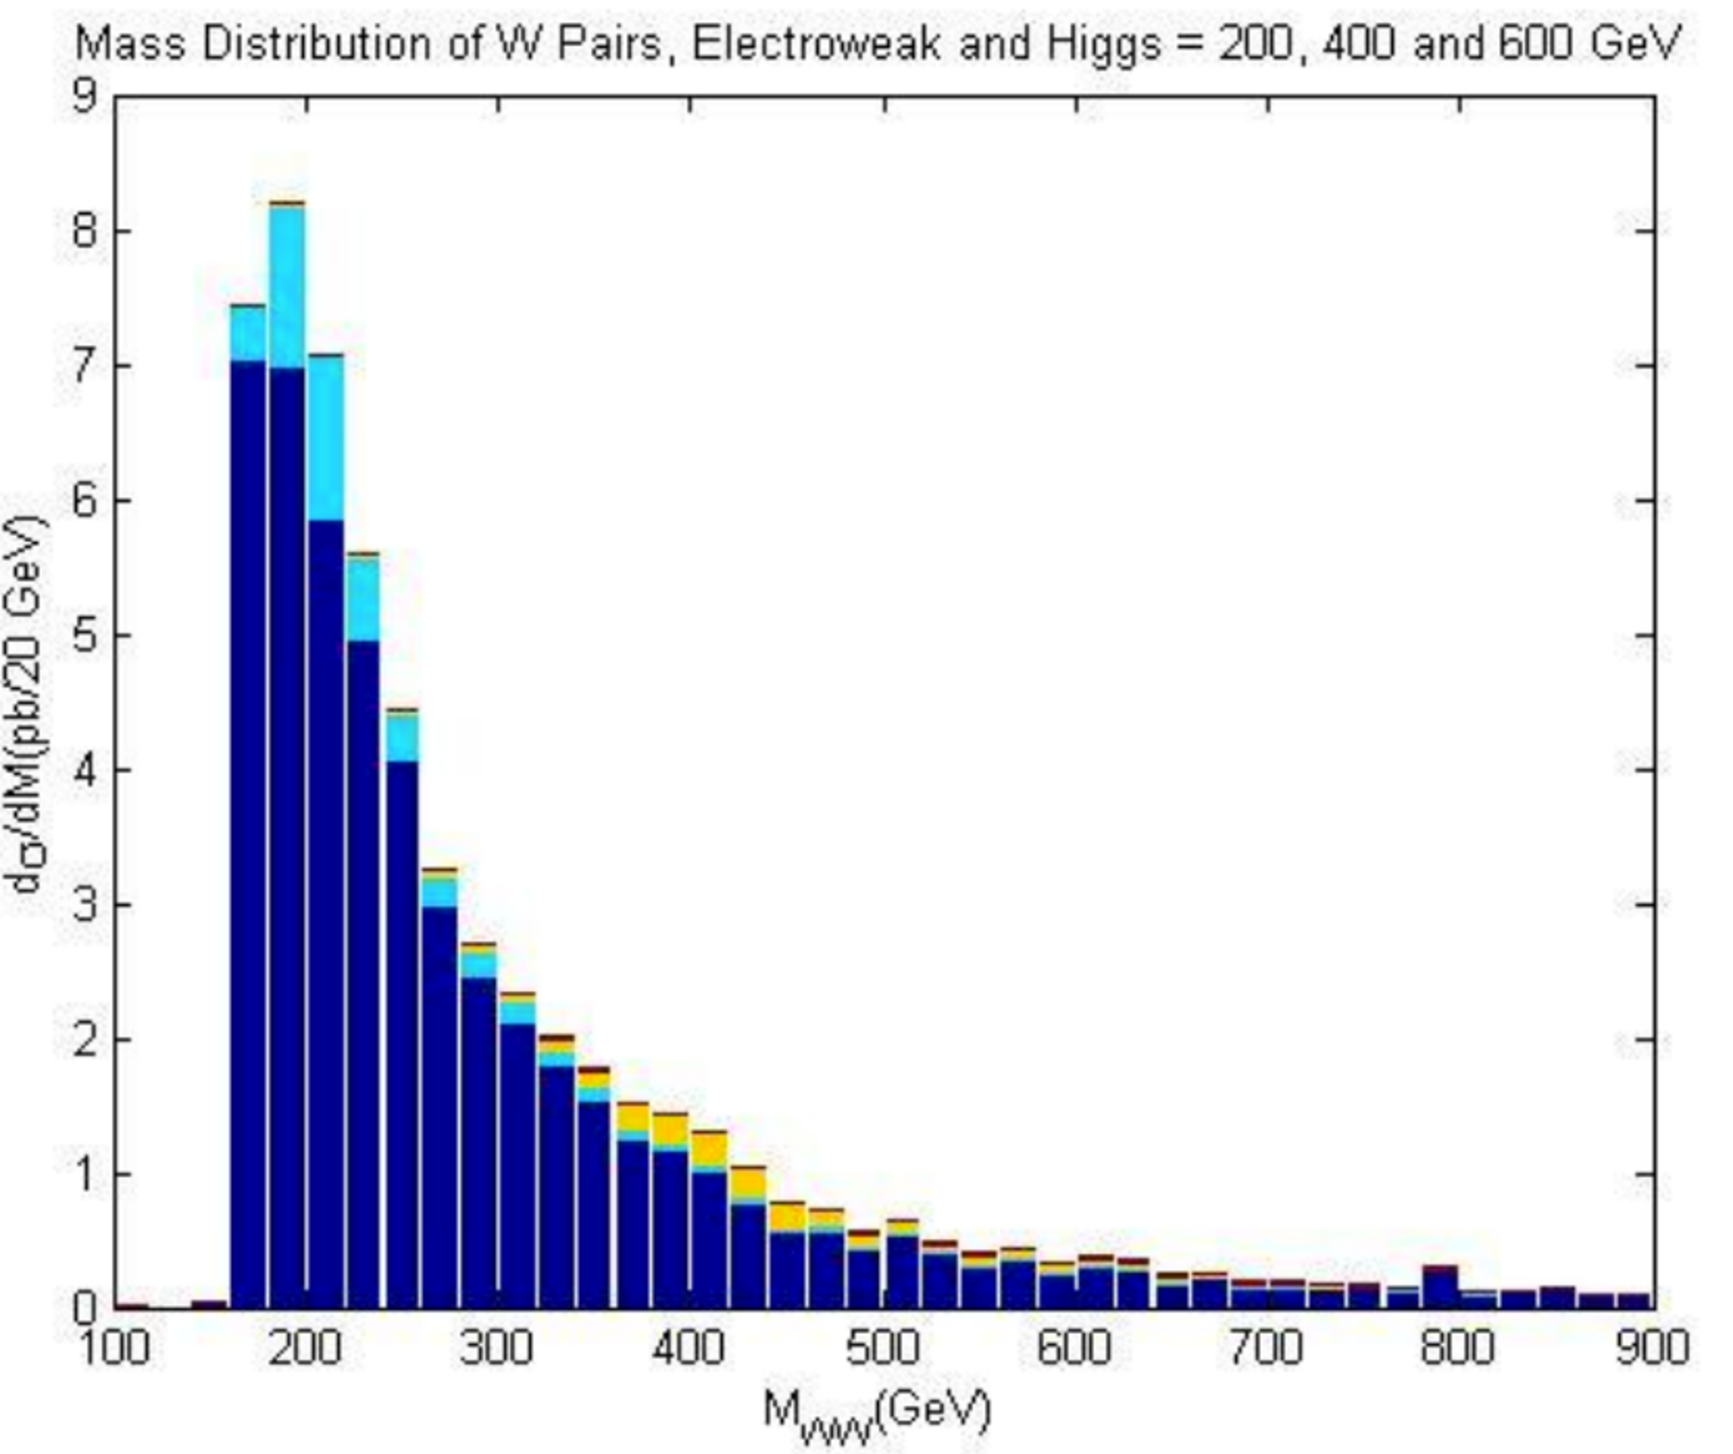
\includegraphics[width=0.5\textwidth]{figs/mwwplot.pdf}
    \caption{Mass spectrum of the $W$ pairs in the $\ell \nu jj$ final
    state for the electroweak continuum (dark blue), and for a 200~GeV
    (light blue), 400~GeV (yellow) and 600~GeV (green) Standard
    Model Higgs boson. The vertical arrows indicate a mass window that
    is used to estimate a simple cut and count limit setting.}
    \label{fig:intor:sig}}
\end{figure}
%%%%%%%%%%%%%%%%%

The assumed cross sections are the inclusive ones~\cite{intor8}, 5.2 pb 
for a 200 GeV Higgs, 2.03 pb and 0.33 pb for a 400 GeV and a 600 GeV Higgs, 
respectively.  The continuum $W$ pair cross section is taken to be 50 pb, 
slightly larger than the Monte Carlo prediction but fully consistent with 
the CMS cross section measurement~\cite{intor3}. The steep fall of the Higgs cross 
section with masses above around 400 GeV mean that the statistical limits 
that can be set with a LHC energy of 7 TeV will be limited to be below that 
mass, even when the most favorable final state is utilized. 



For a simple cut and count experiment, a 200~GeV Higgs has 2.6~pb
within a $\pm 20$~GeV resolution window , while the continuum
background~\cite{intor9} is 13~pb ($S/B \sim$ 0.2). Similarly, a
400~GeV Higgs has 1.0~pb in the $\pm 40$~GeV window of mass
resolution, while there is a 4.3~pb background cross section (S/B
$\sim$ 0.23). For setting a $S$ divided by $\sqrt(B)$ limit of 238.5
total $WW$ events are then needed for a 200~GeV $H$ limit and 872
events are needed for a limit on a 400~GeV H, assuming only
statistical errors.  If there is an additional background of $W$+jets
which is thirty times the electroweak $W$ pair background, then the
limits would rise to 1306 $WW$ events needed at 200 GeV and 4476 $WW$
events at 400 GeV.  To set the required luminosity scale, for
1~$\mathrm{fb}^{-1}$ total integrated luminosity, roughly 10000 $W$
pairs are produced, and 1000 would survive a selection efficiency of
10\%.  The actual luminosity needed to set an exclusion limit will lie
somewhere between the two extremes of irreducible electroweak $WW$
pair production and reducible $W+$jets production.  Note that the
electroweak production of $WZ$ also exists giving the same final state
when the $Z $ decays hadronically.  The dijet mass resolution does not
resolve the $W$ and the $Z$ because of the jet resolution, therefore
the $WZ$ process is included in our accounting of the diboson
background.  The exact limit depends on a proper understanding of the
systematic errors on the $W+$jets background. To achieve that
understanding the jet scale and resolution, which affect the $WW$
fitted yield, were independently determined by examining top
events. The dijet shape uncertainty was determined by fitting
different Monte Carlo samples, which vary scale and matching, to the
dijet data outside the $W$ mass range.  The four body mass spectrum
was determined by using data dijet sidebands to achieve a reasonable
fit to the four body spectrum. This procedure was necessitated by the
failure of the $W+$jets Monte Carlo to represent the data well. The
systematic errors on the data driven four body mass spectrum are
determined in a data driven fashion.


%%%%%%%%%%%%%%%%%%%%%%%%%%%%%%%%%%%%%%%%%%%%%%%%%%%%%%%%%%%%%%%%%%%%%%%%%%%%%%%%%%%%%%%%
%%%%%%%%%%%%%%%%%%%%%%%%%%%%%%%%%%%%%%%%%%%%%%%%%%%%%%%%%%%%%%%%%%%%%%%%%%%%%%%%%%%%%%%%
%%%%%%%%%%%%%%%%%%%%%%%%%%%%%%%%%%%%%%%%%%%%%%%%%%%%%%%%%%%%%%%%%%%%%%%%%%%%%%%%%%%%%%%%
\section{Signal and background expectations from CMS simulation}
\label{sec:MCexpectations}
% ---- ---- ---- ---- ---- ---- ---- ---- ---- ---- --
\subsection {The signal}
The expected production cross-section, multiplied by the branching
fraction of the SM Higgs boson decay into a pair of W bosons
\cite{LHCHiggsCrossSectionWorkingGroup:2011ti} and subsequently into a
lepton-neutrino and di-jet pair translates into the effective
cross-section for the analyzed process, as listed in
Table~\ref{tab:signals} as a function of the Higgs mass.

\begin{table}[htb]
  \begin{center}
  \begin{tabular}{c|c|c}
  \hline
  $m_{\textnormal{H}}$ (\GeV)   & $\sigma_{\textnormal{gg}}$ (pb) & $\sigma_{\textnormal{VBF}}$ (pb) \\
  \hline
%  160 & $2.41  \pm 0.45$          & $0.234^{+0.006}_{-0.006}$\\
  170 & $2.18  \pm 0.39$          & $0.230^{+0.008}_{-0.004}$\\
  180 & $1.85  \pm 0.33$          & $0.204^{+0.006}_{-0.004}$\\
  190 & $1.36  \pm 0.23$          & $0.159^{+0.005}_{-0.003}$\\
  200 & $1.12^{+0.19}_{-0.17}$    & $0.136^{+0.005}_{-0.003}$\\
  250 & $0.67^{+0.11}_{-0.10}$    & $0.087^{+0.003}_{-0.002}$\\
  300 & $0.48^{+0.08}_{-0.07}$    & $0.060^{+0.003}_{-0.002}$\\
  350 & $0.45^{+0.09}_{-0.07}$    & $0.0416^{+0.002}_{-0.0012}$\\
  400 & $0.34^{+0.05}_{-0.06}$    & $0.0272^{+0.0016}_{-0.0008}$\\
  450 & $0.22^{+0.03}_{-0.04}$    & $0.0197^{+0.0013}_{-0.0006}$\\
  500 & $0.13^{+0.02}_{-0.02}$    & $0.0150^{+0.0011}_{-0.0005}$\\
  550 & $0.084^{+0.016}_{-0.015}$ & $0.0117^{+0.0009}_{-0.0004}$\\
  600 & $0.053^{+0.010}_{-0.010}$ & $0.0093^{+0.0008}_{-0.0004}$\\
  \hline
  \end{tabular}
  \end{center}
  \caption{The cross section for the signal, where the branching fractions of the Higgs into WW
  and of each W into leptons are taken into account in the calculation.}
  \label{tab:signals}
\end{table}%

%%%%%%%%%%%%%%%%%%%%%%%%%%%%%
%%%%%%%%%%%
\subsection {The backgrounds}
%%%%%%%%%%%
All processes yielding one lepton, two or more jets, 
and missing transverse energy are possible sources 
of background. The most relevant ones are:
%%%%%%%%%%%
\begin{itemize}
  \item W+jets: this is the production of a single W vector boson 
        in association with quarks or gluons that mimic the final state 
        signature. 
        Because of its large cross section, it is by far the most important 
	background to the analysis.
  \item Drell-Yan Z/$\gamma^{*}$+jets: this is the production of 
        a single Z/$\gamma^{*}$ boson in association with quarks or gluons, 
	where one lepton escapes undetected because of acceptance or 
        inefficiency effects, and the hadronic activity mimics the final 
	 state signature.
  \item WW: this electroweak diboson production is an irreducible 
        background for this analysis. Because its cross-section is measured
	at the LHC, it also serves as a standard candle.
  \item WZ: in case the Z decays hadronically, or the W decays hadronically 
              and one Z lepton is not identified by the detector,
              this sample also contributes to the backgrounds.
  \item ZZ: in case one Z decays hadronically, and one lepton is not identified by the detector,
              this sample contributes to the backgrounds.
  \item $t\bar{t}$: top quarks pairs are produced at LHC via the gluon fusion process
              $gg\to{}t\bar{t}$ or via QCD quark annihilation $q\bar{q}\to{}t\bar{t}$.
              The semi-leptonic component, in which one W decays hadronically,
              is reduced by requiring exactly 2 or 3 jets,
              while the fully leptonic decay mode is reduced by requiring only 
	      one good lepton in the event.
              However, because of acceptance and inefficiencies, 
              this background still contaminates the signal.
  \item Single top production: it proceeds through three separate channels:
       \begin{enumerate}
         \item t-channel: top is produced after a quark-gluon interaction 
               with the exchange of a virtual W.
         \item s-channel: top is produced in association with an anti-bottom, 
               after the annihilation of a pair of quarks in a weak vertex.
         \item tW-channel: top is produced in association with a charged vector boson in a weak process, 
               from a gluon-bottom pair in the initial state.
       \end{enumerate}
%       The first two can be distinguished from signal thanks to a selection on the energy of b-quarks, 
%       which are quite different from signal tag quarks, while tW-channel has got a missing jet.
  \item QCD multi-jet events generate a background 
       because of the non-negligible probability of jets to be reconstructed as leptons.
\end{itemize}
%%%%%%%%%%%%%%%%%%%%%%
The cross section for the backgrounds, multiplied by the branching ratio when meaningful, 
are reported in Table~\ref{tab:bkg_XS}. 
%%%%%%%%%%%
\begin{table}[htb]
  \begin{center}
  \begin{tabular}{c|c}
  \hline
  Channel & Cross-section (pb) \\
  \hline
  W+jets                        & 31314   \\ %  $\pm$ 1600  \\
  Z+jets                        & 3050    \\ %  $\pm$ 130 \\
  WW                            & 43      \\ %  $\pm$ 1.5 \\
  WZ                            & 18.2    \\ %  $\pm$ 0.7\\
  ZZ                            & 5.90    \\ %  $\pm$ 0.15\\
  t$\bar{\textnormal{t}}$+jets  & 157.5   \\ %  $\pm$ 10 \\
  t+jets ($t$-channel)          & 64.6    \\ % $\pm$ 0.05 \\
  t+jets ($s$-channel)          & 4.6     \\ % $\pm$ 1.1 \\
  t+jets ($t$W-channel)         & 15.7    \\ % $\pm$ 0.8 \\
  QCD (ele enriched)            & 6740000 \\ % $\pm$ \\
  QCD (mu enriched)             & 84700   \\ % $\pm$ \\
  \hline
  \end{tabular}
  \end{center}
  \caption{The cross section for the backgrounds, multiplied by the branching ratio when meaningful.
  Each different sample notation includes all the decays taken into account in the calculation.}
  \label{tab:bkg_XS}
\end{table}%
%
%\begin{table}[htb]
%  \begin{center}
%  \begin{tabular}{c|c}
%  \hline  \hline
%  Channel & Cross-section (pb) \\
%  \hline
%  W+jets                        & 31300   $\pm$ 1600 \\
%  Z+jets                        & 3050    $\pm$  130 \\
%  WW                            & 43.0    $\pm$ 1.5  \\
%  WZ                            & $18.2   $\pm$ 0.7  \\
%  ZZ                            & 5.90    $\pm$ 0.15 \\
%  t$\bar{\textnormal{t}}$+jets  & 157.5   $\pm$   10 \\
%  t+jets ($s$-channel)          & 4.63    $\pm$ 0.19 \\
%  t+jets ($t$-channel)          & 64.57   $\pm$ 2.58 \\
%  t+jets ($t$W-channel)         & 15.74   $\pm$ 1.17 \\
%  QCD (ele enriched)            & 6740000 $\pm$ 100\%\\
%  QCD (mu enriched)             & 84700 $\pm$  100\%\\
%  \hline  \hline
%  \end{tabular}
%  \end{center}
%  \caption{The cross section for the backgrounds, multiplied by the branching ratio when meaningful.}
%  \label{tab:bkg_XS}
%\end{table}%
%%%%%%%%%%%%
%%%%%%%%%%%%%%%%%%%%%%%%%%%%%%%%%%%%%%%%%%%%
\section{Datasets}
\label{sec:technicalities}
% ---- ---- ---- ---- ---- ---- ---- ---- ---- ---- ---- ---- --
\subsection{Data samples}
The data samples used in this analysis were recorded by the CMS experiment in 2010 and 2011.
Only certified runs and luminosity sections are considered, which means that a good functioning
of all CMS sub-detectors is required. The total statistics analyzed correspond to an integrated
luminosity of about $5.0\fbinv$.
% The analysis relies on centrally-produced Primary Datasets (PDs), each of which consists of a collection
% of High Level Trigger (HLT) paths. As explained in Section~\ref{sec:trigger}, single-lepton triggers
% are used to select the events interesting for this analysis in both
% the $e$ and $\mu$ channels, up to an instantaneous luminosity $L \sim 1\cdot10^{33}\percms$. At higher
% luminosities, we move to cross electron+di-jet triggers for the $e$ channel to cope with the
% unsustainable single-electron HLT rate. Therefore, the analysis relies on the so-called ``SingleElectron''
% and ``SingleMu'' PDs for the first data-taking period, and on the ``ElectronHad'' and ``SingleMu'' ones 
% for the most runs. 
The datasets used for the analysis and the corresponding run ranges are listed in Table~\ref{tab:datasets}.
All data samples were reconstructed using a \texttt{CMSSW\_4\_2\_X} release version.
%%%%%%%%%%%
\begin{table}[htb]
  \begin{center}
  \begin{tabular}{r|r}
  \hline  \hline
  Dataset name & Run range \\
  \hline
  /EG/Run2010A-Apr21ReReco-v1/AOD   & 136033 - 144114  \\
  /Mu/Run2010A-Apr21ReReco-v1/AOD   &            \\ 
  \hline
  /Electron/Run2010B-Apr21ReReco-v1/AOD   &  144919 - 149442  \\
  /Mu/Run2010B-Apr21ReReco-v1/AOD         &             \\
  \hline
  /SingleElectron/Run2011A-May10ReReco-v1/AOD   & 160431 - 163869 \\
  /SingleMu/Run2011A-May10ReReco-v1/AOD         &                 \\
  \hline                                     
  /SingleElectron/Run2011A-PromptReco-v4/AOD       & 165088 - 167913   \\
  /SingleMu/Run2011A-PromptReco-v4/AOD          &                 \\
  \hline                                     
  /SingleElectron/Run2011A-05Aug2011-v1/AOD        & 170826 - 172619 \\
  /SingleMu/Run2011A-05Aug2011-v1/AOD           &                 \\
  \hline                                     
  /SingleElectron/Run2011A-PromptReco-v6/AOD       & 172620 - 173692 \\
  /SingleMu/Run2011A-PromptReco-v6/AOD          &                 \\
  \hline                                     
  /SingleElectron/Run2011B-PromptReco-v1/AOD       & 175832 - 180252 \\
 /SingleMu/Run2011B-PromptReco-v1/AOD          &                 \\
  \hline  \hline
  \end{tabular}
  \end{center}
  \caption{Summary of the data samples used and the run ranges of applicability.}
  \label{tab:datasets}
\end{table}%
%%%%%%%%%%%
%%%%%%%%%%%%%%%%%%%%%%%%%%%%%%%%%%%%%%%%%%%%
\subsection{Monte Carlo samples}
Standard Model Higgs boson samples, 
as well as samples for a large variety of electroweak and QCD-induced background sources, 
have been generated and showered using different Monte Carlo generators.
To better reproduce the actual data-taking conditions, where there is a significant probability
that more than two protons interact in the same bunch crossing, pile-up (PU) events are
added on top of the hard scattering. Particle interactions with the detector were reproduced through
a detailed description of CMS.

The POWHEG-BOX generator \cite{Nason:2004rx,Frixione:2007vw,Alioli:2010xd,Nason:2009ai} has been used to
produce Higgs signal events, and the showering has been performed with PYTHIA6 \cite{pythia}. For this analysis, 
samples with Higgs mass hypotheses ranging from 170 to 600\GeV have been used.
 

The background and signal samples used for the studies are listed in Table~\ref{tab:MCsamples},
together with the equivalent luminosity available for the study.
All background MC samples considered in this analysis come from 
the official ``Fall11'' production. Events were
reconstructed making use of a \texttt{CMSSW\_4\_2\_X} release version. 
% The pile-up scenario used for
% these samples consists of a flat distribution of PU events up to ten additional interactions on top
% of the hard scattering plus a poissonian tail with a mean of ten interactions; only pile-up occurring 
% in the same bunch crossing of the main event (in time PU) was considered.
%%%%%%%%%%%%%%%%%%%%%%%%%%%%%%%%%
\begin{sidewaystable}[htb]
  \begin{center}
    \begin{tabular}{l} 
      \hline\hline
      sample \\
      \hline
      /WJetsToLNu\_TuneZ2\_7TeV-madgraph-tauola/Fall11-PU\_S6\_START42\_V14B-v1/AODSIM    \\
      /WW\_TuneZ2\_7TeV\_pythia6\_tauola/Fall11-PU\_S6\_START42\_V14B-v1/AODSIM     \\
      /WZ\_TuneZ2\_7TeV\_pythia6\_tauola/Fall11-PU\_S6\_START42\_V14B-v1/AODSIM     \\
      /TTJets\_TuneZ2\_7TeV-madgraph-tauola/Fall11-PU\_S6\_START42\_V14B-v2/AODSIM    \\
      /QCD\_Pt-20\_MuEnrichedPt-15\_TuneZ2\_7TeV-pythia6/Fall11-PU\_S6\_START42\_V14B-v2/AODSIM  \\      
      /DYJetsToLL\_TuneZ2\_M-50\_7TeV-madgraph-tauola/Fall11-PU\_S6\_START42\_V14B-v1/AODSIM   \\
      /Tbar\_TuneZ2\_s-channel\_7TeV-powheg-tauola/Fall11-PU\_S6\_START42\_V14B-v1/AODSIM     \\
      /Tbar\_TuneZ2\_t-channel\_7TeV-powheg-tauola/Fall11-PU\_S6\_START42\_V14B-v1/AODSIM     \\
      /Tbar\_TuneZ2\_tW-channel-DS\_7TeV-powheg-tauola/Fall11-PU\_S6\_START42\_V14B-v1/AODSIM    \\
      /T\_TuneZ2\_s-channel\_7TeV-powheg-tauola/Fall11-PU\_S6\_START42\_V14B-v1/AODSIM     \\
      /T\_TuneZ2\_t-channel\_7TeV-powheg-tauola/Fall11-PU\_S6\_START42\_V14B-v1/AODSIM     \\
      /T\_TuneZ2\_tW-channel-DS\_7TeV-powheg-tauola/Fall11-PU\_S6\_START42\_V14B-v1/AODSIM     \\
%      \hline
%      /QCD\_Pt-20to30\_EMEnriched\_TuneZ2\_7TeV-pythia/Summer11-PU\_S4\_START42\_V11-v1/AODSIM\\
%      /QCD\_Pt-30to80\_EMEnriched\_TuneZ2\_7TeV-pythia/Summer11-PU\_S4\_START42\_V11-v1/AODSIM\\
%      /QCD\_Pt-80to170\_EMEnriched\_TuneZ2\_7TeV-pythia6/Summer11-PU\_S4\_START42\_V11-v1/AODSIM \\
%      /QCD\_Pt-20to30\_BCtoE\_TuneZ2\_7TeV-pythia6/Summer11-PU\_S4\_START42\_V11-v1/AODSIM \\
%      /QCD\_Pt-30to80\_BCtoE\_TuneZ2\_7TeV-pythia6/Summer11-PU\_S4\_START42\_V11-v1/AODSIM \\
%      /QCD\_Pt-80to170\_BCtoE\_TuneZ2\_7TeV-pythia/Summer11-PU\_S4\_START42\_V11-v1/AODSIM   \\
      \hline
      /WJetsToLNu\_TuneZ2\_matchingdown\_7TeV-madgraph-tauola/Summer11-PU\_S4\_START42\_V11-v1/AODSIM  \\
      /WJetsToLNu\_TuneZ2\_matchingup\_7TeV-madgraph-tauola/Summer11-PU\_S4\_START42\_V11-v1/AODSIM  \\
      /WJetsToLNu\_TuneZ2\_scaledown\_7TeV-madgraph-tauola/Summer11-PU\_S4\_START42\_V11-v1/AODSIM          \\
      /WJetsToLNu\_TuneZ2\_scaleup\_7TeV-madgraph-tauola/Summer11-PU\_S4\_START42\_V11-v1/AODSIM            \\
      /WToLNu\_1jEnh2\_2jEnh35\_3jEnh40\_4jEnh50\_7TeV-sherpa/Summer11-PU\_S4\_START42\_V11-v1/AODSIM      \\
      \hline 
      /GluGluToHToWWToLNuQQ\_M-*\_7TeV-powheg-pythia6/Fall11-PU\_S6\_START42\_V14B-v1/AODSIM  \\
      /VBF\_HToWWToLNuQQ\_M-*\_7TeV-powheg-pythia6/Fall11-PU\_S6\_START42\_V14B-v1/AODSIM \\
      Higgs mass from 170 to 600~GeV   \\
      \hline\hline
    \end{tabular}
  \end{center}
  \caption{Summary of Monte Carlo samples used in the analysis for background and signal modeling and for systematic studies.}
  \label{tab:datasets:mcstat}
  %FIXME add the corresponding cross-sections
  \label{tab:MCsamples}
\end{sidewaystable}
%%%%%%%%%%%%%%%%%%%%%%%%%%%%%%%%%
\clearpage
%%%%%%%%%%%%%%%%%%%%%%%%%%%%%%%%%%%%%%%%%%%%%%%%%%
%%%%%%%%%%%%%%%%%%%%%%%%%%%%%%%%%%%%%%%%%%%%%%%%%%
%%%%%%%%%%%%%%%%%%%%%%%%%%%%%%%%%%%%%%%%%%%%%%%%%%
%%%%%%%%%%%%%%%%%%%%%%%%%%%%%%%%%%%%%%%%%%%%%%%%%%
\section{Physics objects reconstruction}
\label{sec:reco}
\label{sec:firstStep}
% ---- ---- ---- ---- ---- ---- ---- ---- ---- ---- ---- ---- ---- ---- ----
The event selection criteria are described in detail in AN-11/110, Section 4. 
Here we summarize them in brief.

%%%%%%%%%%%%%%%%%%%%%%%%%%%%
\subsection{Electron selection}
\label{sec:electron_cuts}

Electrons are reconstructed using a gaussian sum 
filter (GSF) algorithm \cite{CMS-PAS-EGM-10-004},
and are required to pass electron ID cuts according 
to the simple cut-based electron ID~\cite{simplecutbasedelectronid}, 
with the ``VBTF Working Point 70''. 
The GSF algorithm accounts for possible energy loss due to
bremsstrahlung in the tracker layers.
The energy of an electron candidate with $\et>35~\gev$ is essentially
determined by the ECAL cluster energy, while its momentum direction
is determined by that of the associated track.
The simple cut based electron ID relies on three shower
shape variables with different cut values for the barrel and
the endcap regions, as shown in Table~\ref{tab:EleID}.

Additionally, we require
%%%%%%%%%%%%%%%%%%%
\begin{itemize}
\item Electron $E_\mathrm{T} > 35\,\mathrm{GeV}$.
\item Pseudorapidity $|\eta| < 2.5$. There is an exclusion range due
        to the ECAL barrel-endcap transition region, defined by
        $1.4442 < |\eta_{\mathrm{sc}}| < 1.566$, where
        $\eta_{\mathrm{sc}}$ is the pseudorapidity of the ECAL
        supercluster.
\item Impact parameter: We cut on the absolute value of the impact
       parameter calculated with respect to the average beamspot. We
       require:  $d_0(\mathrm{Bsp}) < 0.02\,\mathrm{cm}.$   
\item The selected electron candidates have to be isolated simultaneously in
the tracker, and in the electromagnetic and hadronic calorimeters.  Combined
relative isolation is defined as
%%%
\begin{equation*}
\mathrm{RelIso_{\mathrm{Comb}}} = \frac{I_{\mathrm{Trk}}+I_{\mathrm{EM}}+I_{\mathrm{had}}}{E_\mathrm{T}}.
\end{equation*} 
%%%
The electron candidate is required to have 
$\mathrm{RelIso_{\mathrm{Comb}}} < 0.05$ in order 
to be considered isolated. 
A pile-up offset subtraction in the isolation cone 
using fastjet algorithm \cite{FastJetPUSubtraction} is applied.
We also veto the presence of a second loose lepton in the event.
\item 
In order to reject events in which the electron candidate actually
originates from a conversion of a photon into an $e^{+}e^{-}$ pair, we
require the number of missed inner tracker layers of the electron
track to be exactly zero (i.e. there are no missed layers before the
first hit of the electron track from the beam line). In addition, we
reject any event in which the selected electron is flagged as a
conversion, \textit{i.e.}, an electron that has a 
distance of the partner track $|$\texttt{dist}$|$ $< 0.02$~mm and an
opening angle $|$\texttt{dcot}$|$ $< 0.02$~\cite{ConversionRejection}.
\end{itemize}
%%%%%%%%%%%%%%%%%%%
%%%%%%%%%%%%%%%%%%%
%%%%%%%%%%%%%%%%%%%
\begin{table}[bthp]
\begin{center}
{\footnotesize
\begin{tabular}{|c|c|c|c|c|}
\hline
ID Variable & WP70 Barrel & WP70 Endcaps & WP95 Barrel & WP95 Endcaps  \\
\hline
$\sigma_{i\eta i\eta}$ & 0.01 & 0.03 & 0.01 & 0.03 \\
$\phi_{\mathrm{SC}} - \phi_{\mathrm{trk}}$ & 0.03 & 0.02 & 0.8 & 0.7 \\
$\eta_{\mathrm{SC}} - \eta_{\mathrm{trk}}$ & 0.004 & 0.005 & 0.007 & 0.01 \\
\hline
\end{tabular}
\caption[.]{\label{tab:EleID} Cut values for electron identification
variables for VBTF Working Point (WP) 70 (barrel and endcap), as used
for the tight electron selection, and VBTF Working Point (WP) 95
(barrel and endcap), as used in the loose electron selection.}}
\end{center}
\end{table}
%%%%%%%%%%%%%%%%%%%
%%%%%%%%%%%%%%%%%%%%%%%%%%%%%%%%%%%%%%%%%%%%%%%%%%%%%%%%%%%%%%%%%%%%%%%%%%%%
%%%%%%%%%%%%%%%%%%%%%%%%%%%%%%%%%%%%%%%%%%%%%%%%%%%%%%%%%%%%%%%%%%%%%%%%%%%%
\subsection{Muon selection}
\label{sec:muon_cuts}
Muon candidates are identified by two different 
algorithms~\cite{MUONPAS}: one proceeds from the inner tracker outwards, 
the other one starts from tracks measured in the muon chambers and matches 
and combines them with tracks reconstructed in the inner tracker. 
These selection criteria are summarized below:
%%%%%%%%%%%%%%%%%%%
\begin{itemize}
\item The muon candidate is reconstructed both as a global muon and
as a tracker muon.
\item The number of hits of the muon track in the silicon tracker has
to be $N_{\mathrm{Hits}} > 10$.
\item Number of pixel hits of the Tracker track $\ge 1$;
\item Number of muon hits of the Global track $\ge 2$;
\item Normalized $\chi^{2}$ of the Global track $< 10.0$.
\item Muon $p_{\mathrm{T}} > 25\,\mathrm{GeV}$.
\item Pseudorapidity $|\eta| < 2.1$.
\item Impact parameter: We cut on the absolute value of the impact
parameter calculated with respect to the beamspot. We require:
$d_0(\mathrm{Bsp}) < 0.02\,\mathrm{cm}.$
\item In order to make sure that the selected muon and the selected
jets come from the same hard interaction and not from pile up events,
we require that the $z$ coordinate of the PV of the event and the $z$
coordinate of the muon's inner track vertex lie within a distance of
less than 1~cm.
\item The selected muon candidates also have to be isolated.
We require the muon to be isolated simultaneously in the
tracker, and in the electromagnetic and hadronic calorimeters.  
The muon candidate is required to have
$\mathrm{RelIso_{\mathrm{Comb}}} < 0.1$ in order to be considered
isolated.
We also veto the presence of a second loose lepton in the event.
\end{itemize}
%%%%%%%%%%%%%%%%%%%%%%%%%%%%
%%%%%%%%%%%%%%%%%%%%%%%%%%%%
%%%%%%%%%%%%%%%%%%%%%%%%%%%%%%%%%%%%%%%%%%%%%%%%%%%%%%%%%%%%%%%%%%%%%%%%%%%%
%%%%%%%%%%%%%%%%%%%%%%%%%%%%%%%%%%%%%%%%%%%%%%%%%%%%%%%%%%%%%%%%%%%%%%%%%%%%

\subsection{Loose Electron}
For the purposes of rejecting events with more than one lepton we
define a loose electron, which has looser cuts. We consider electrons
which have $p_{\mathrm{T}} > 15\,\mathrm{GeV}/c$, $|\eta| < 2.5$, and
$\mathrm{RelIso_{\mathrm{Trk}}} < 0.2$ and which satisfy electron ID
cuts according to ``VBTF Working Point 95'' to be ``loose''. The cut
values for the electron ID variables used in the analysis can be found
in table~\ref{tab:EleID}.

\subsection{Loose Muon}
Additionally, to reject events with more than one lepton, we define a
loose muon, which has looser cuts. We consider all global muons which
have $p_{\mathrm{T}} > 10\,\mathrm{GeV}/c$, $|\eta| < 2.5$, and
$\mathrm{RelIso_{\mathrm{Trk}}} < 0.2$ to be loose muons.

\subsection{Jet selection}
\label{sec:firstStep_jets}
Jets are reconstructed with the anti-KT algorithm \cite{cacciari}, 
starting from the set of objects reconstructed by the particle 
flow \cite{pflow,CMS-PAS-JME-10-003,CMS-PAS-PFT-10-002}.
Jets are corrected such that the measured energy of the jet 
correctly reproduces the energy of the initial particle. 
The CMS standard L2 (relative) correction makes the jet response flat in $\eta$.
The standard L3 (absolute) correction brings the jet closer to the $\PT$ of 
a matched generated jet created using generator level input and a similar 
jet clustering algorithm.
The L2 and L3 corrections are calculated using Monte Carlo, and thus a 
L2L3 residual correction is applied that fixes the discrepancies between 
Monte Carlo and data~\cite{newjes-cms}.
In this analysis we use jets with measured (corrected) $\PT$  
greater than 30~$\gev$. 
We require $|\eta| < 2.4$ so that the jets fall within the
tracker acceptance.  
Jets are required to pass a set of loose identification
criteria; this requirement eliminates jets originating from or being seeded by
noisy channels in the calorimeter~\cite{Chatrchyan:2009hy}: 
%%%%%%%%%%%%%%
\begin{itemize}
\item Fraction of energy due to neutral hadrons $<$ 0.99.
\item Fraction of energy due to neutral EM deposits $<$ 0.99.
\item Number of constituents $>$ 1.
\item Number of charged hadrons candidates $>$ 0.
\item Fraction of energy due to charged hadrons candidates $>$ 0.
\item Fraction of energy due to charged EM deposits $<$ 0.99.
\end{itemize}
%%%%%%%%%%
All energy fractions are calculated from uncorrected jets.

\par
In order to account for electron and muon objects that
have been reconstructed as jets, we remove from the jet
collection any jet that falls within a
cone of radius $R= 0.3$ of a loose electron or a loose muon. 
This ``cleaning'' procedure is applied in order to ensure that the same
particle is not double counted as two different physics objects.
We require exactly two or three jets in the event.

%%%%%%%%%%%%%%%%%%%%%%%%%%%%%%%%%%%%%%%%%%%%%%%%%%%%%%
%%%%%%%%%%%%%%%%%%%%%%%%%%%%%%%%%%%%%%%%%%%%%%%%%%%%%%
\subsection{Missing transverse energy requirement}
\label{sec:MET}
An accurate MET measurement is essential for distinguishing
the $\Wo$ signal from QCD backgrounds. 
We use the MET estimate provided by the Particle Flow algorithm.
PF MET showed the best performance
among several MET algorithms~\cite{PFMET}.
The MET is computed as the vector sum of all PF objects.
A good agreement is found between the MET
distributions of $\Wln$ events in data and simulation~\cite{metPAS}.
The resolution for inclusive multi-jet samples and for
$\Wln$ events is also well reproduced by the simulation.  
A relative broadening of a few percent is observed in the data compared to MC,  
and has a negligible impact on the
extraction of the W yields~\cite{WZCMS:2010}.

We require the event to have missing transverse energy
MET in excess of 25~GeV in case of muon sample and 
30 GeV in case of electron sample.
We also require W transverse mass $ > 50\,\mathrm{GeV}$.
These cuts are designed to reduce the background
from QCD multijet production.
%%%%%%%%%%%%%%%%%%%%%%%%%%%%%%%%%%%%%%%%%%%%%%%%%%%%%%
%%%%%%%%%%%%%%%%%%%%%%%%%%%%%%%%%%%%%%%%%%%%%%%%%%%%%%
%%%%%%%%%%%%%%%%%%%%%%%%%%%%%%%%%%%%%%
%%%%%%%%%%%%%%%%%%%%%%%%%%%%%%%%%%%%%%
%%%%%%%%%%%%%%%%%%%%%%%%%%%%%%%%%%%%%%%%%%%%%%%%%%%%%%%%%%%%%%%%%%%%
%%%%%%%%%%%%%%%%%%%%%%%%%%%%%%%%%%%%%%%%%%%%%%%%%%%%%%%%%%%%%%%%%%%%
%%%%%%%%%%%%%%%%%%%%%%%%%%%%%%%%%%%%%%%%%%%%%%%%%%%%%%%%%%%%%%%%%%%%
\section{Lepton reconstruction and selection efficiency}
\label{sec:efficiency}
The lepton efficiency and data/MC scale factors computed using 
the ``tag \& probe'' technique are described in detail in the CMS analysis note 
AN-2012/021.
%%%%%%%%%%%%%%%%%%%%%%%%%%%%%%%%%%%%%%%%%%%%%%%%%%%%%%%%%%%%%%%%%%%%
%%%%%%%%%%%%%%%%%%%%%%%%%%%%%%%%%%%%%%%%%%%%%%%%%%%%%%%%%%%%%%%%%%%%
%%%%%%%%%%%%%%%%%%%%%%%%%%%%%%%%%%%%%%%%%%%%%%%%%%%%%%%%%%%%%%%%%%%%
\section{Trigger selection and efficiency}
\label{sec:trigger}
The trigger selection used in this analysis and the trigger efficiency 
computation are also described in detail in the CMS analysis note 
AN-2012/021.
%%%%%%%%%%%%%%%%%%%%%%%%%%%%%%%
%%%%%%%%%%%%%%%%%%%%%%%%%%%%%%%

\section{Comparison of Data and Monte Carlo simulation}
To assess the quality of the modeling provided by the MC simulation we 
make comparisons between the MC shape normalized to the total
prediction for the background compared to the overall data
yield after applying the event selection criteria. 
We show the distributions of various kinematic
variables after applying all the selection cuts in 
Figures ~\ref{fig:mu_jet_pt}-\ref{fig:mu_mjj}
for the muon+jets sample and in 
Figures ~\ref{fig:elec_jet_pt}-\ref{fig:elec_mjj} for
the electron+jets sample. The MC has been been corrected for
lepton reconstruction and selection efficiency and the trigger efficiency.
Seeing reasonable agreement gives us confidence in
the qualitative aspects of the MC modeling. 
%%%%%%%%%%%%%%%%%%%%%%%%%%%%
\begin{figure}[ht]
  {\centering
    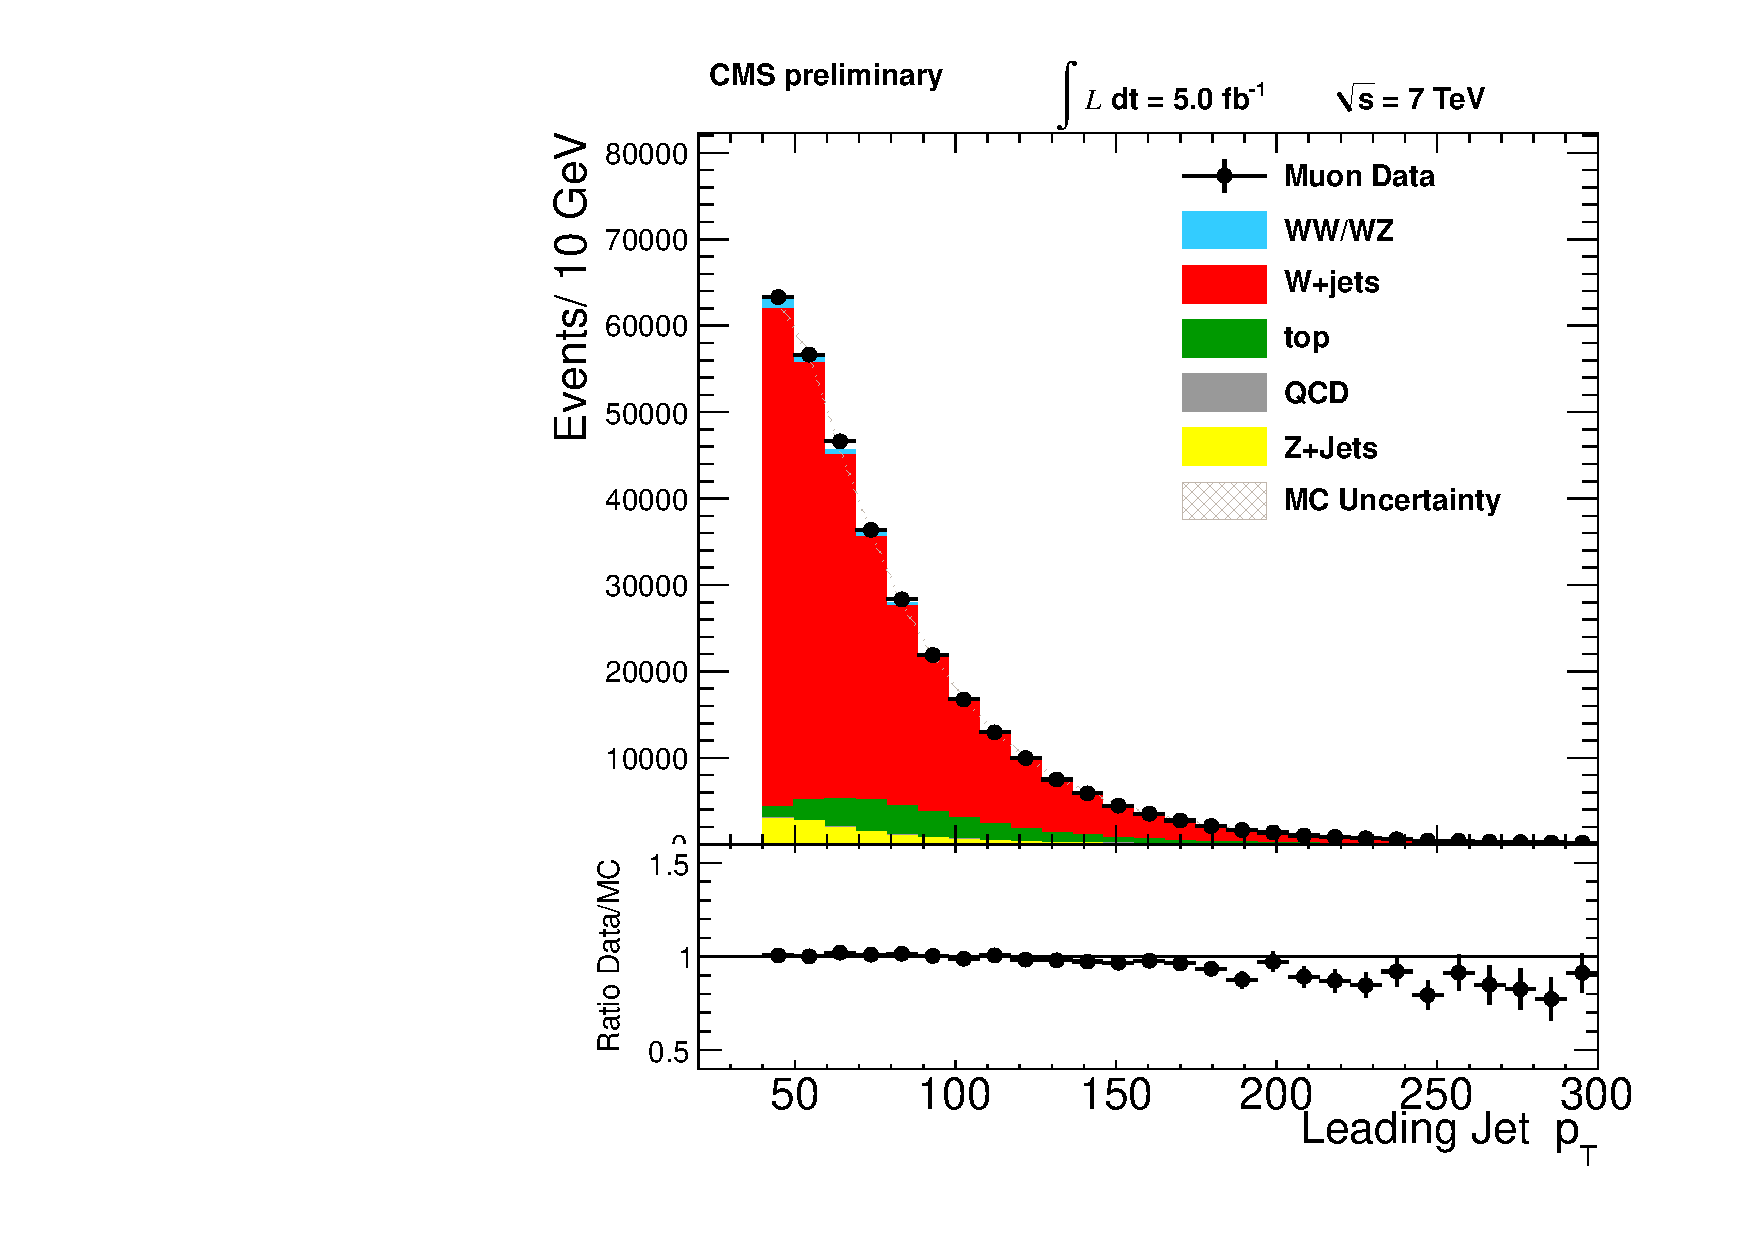
\includegraphics[width=0.49\textwidth]{figs/n-1_plots_mu/mu_jetld_pt.pdf}
    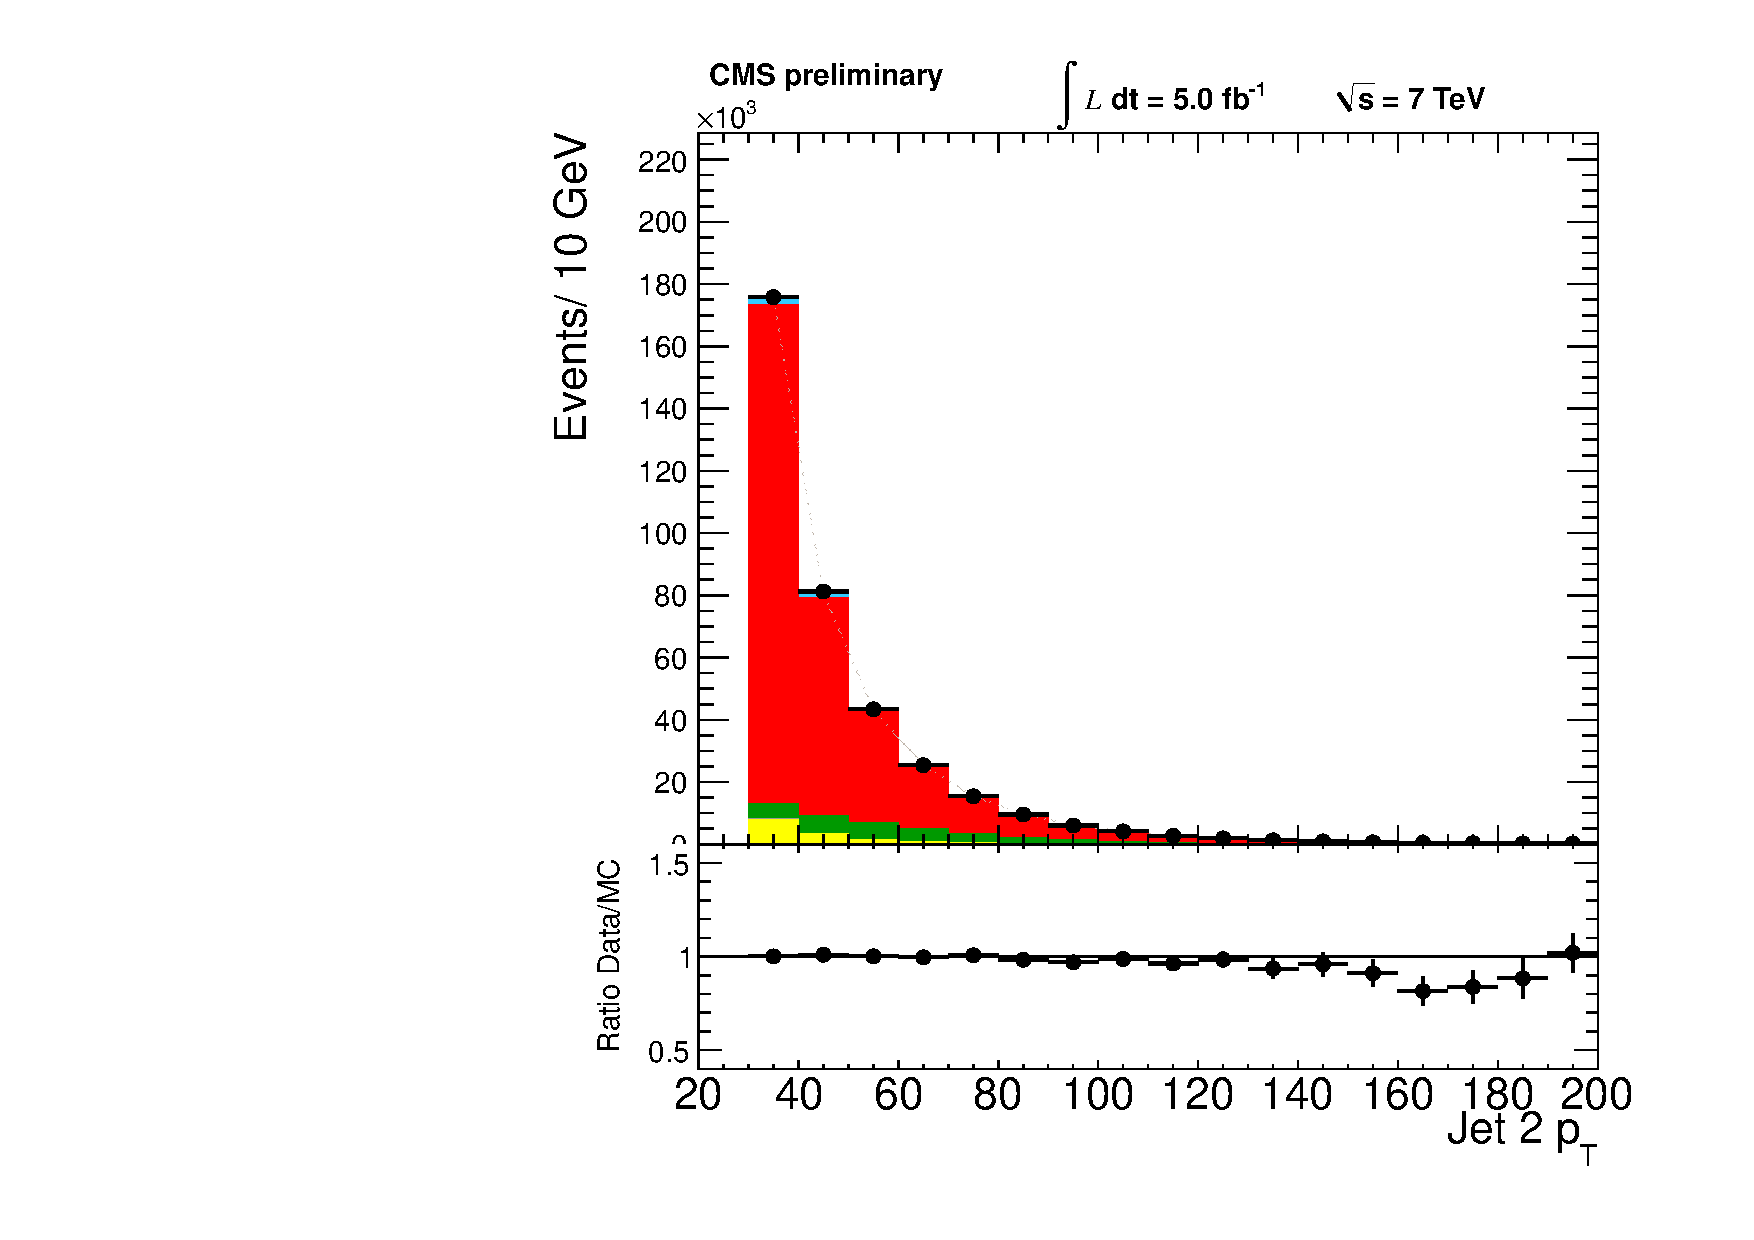
\includegraphics[width=0.49\textwidth]{figs/n-1_plots_mu/mu_jetnt_pt.pdf}
    \caption{Comparison of the leading jet (left) and 
      the second jet (right) $p_{T}$ distributions from data and MC for the muon+jets
      selection.}
    \label{fig:mu_jet_pt}}
\end{figure}
%%%%%%%%%%%%%%%%%%%%%%%%%%%%
\begin{figure}[h!t]
  {\centering
    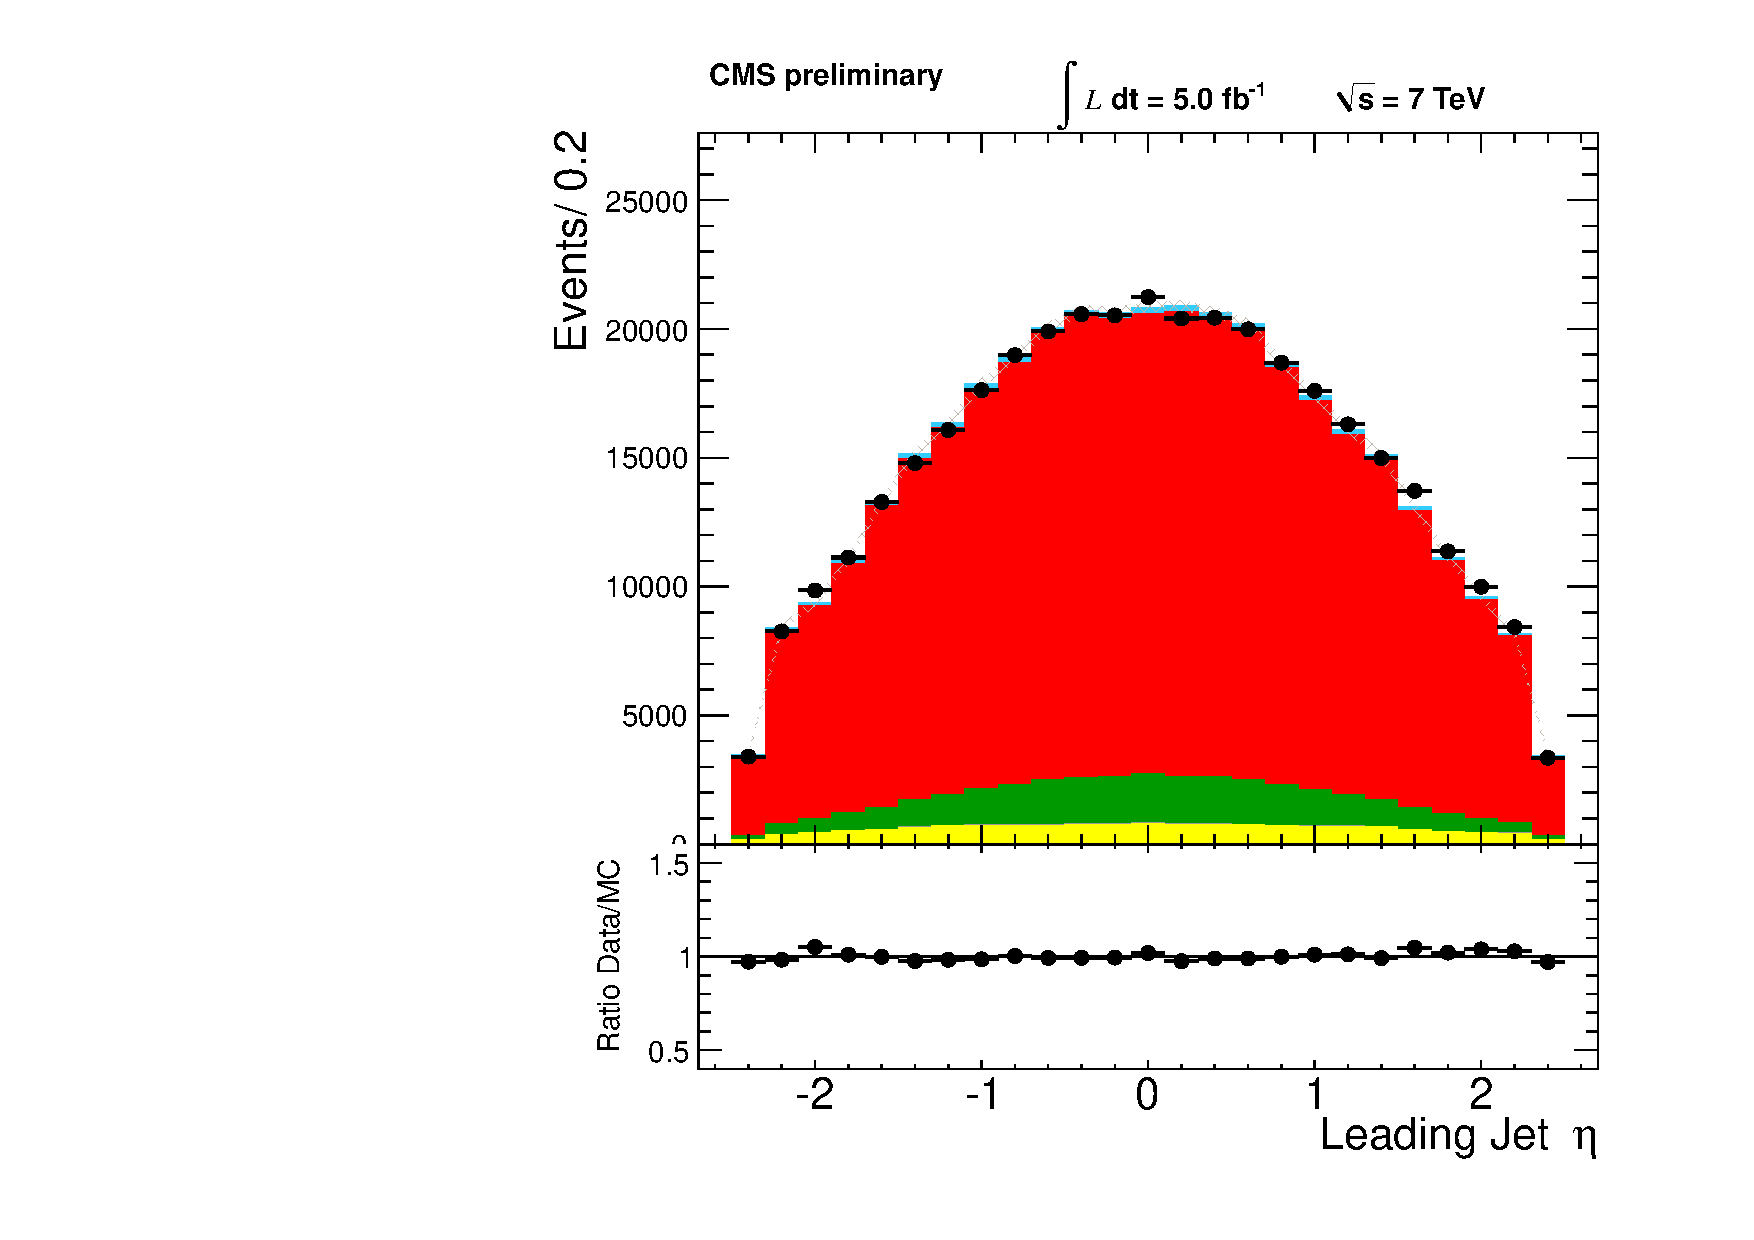
\includegraphics[width=0.49\textwidth]{figs/n-1_plots_mu/mu_jetld_eta.pdf}
    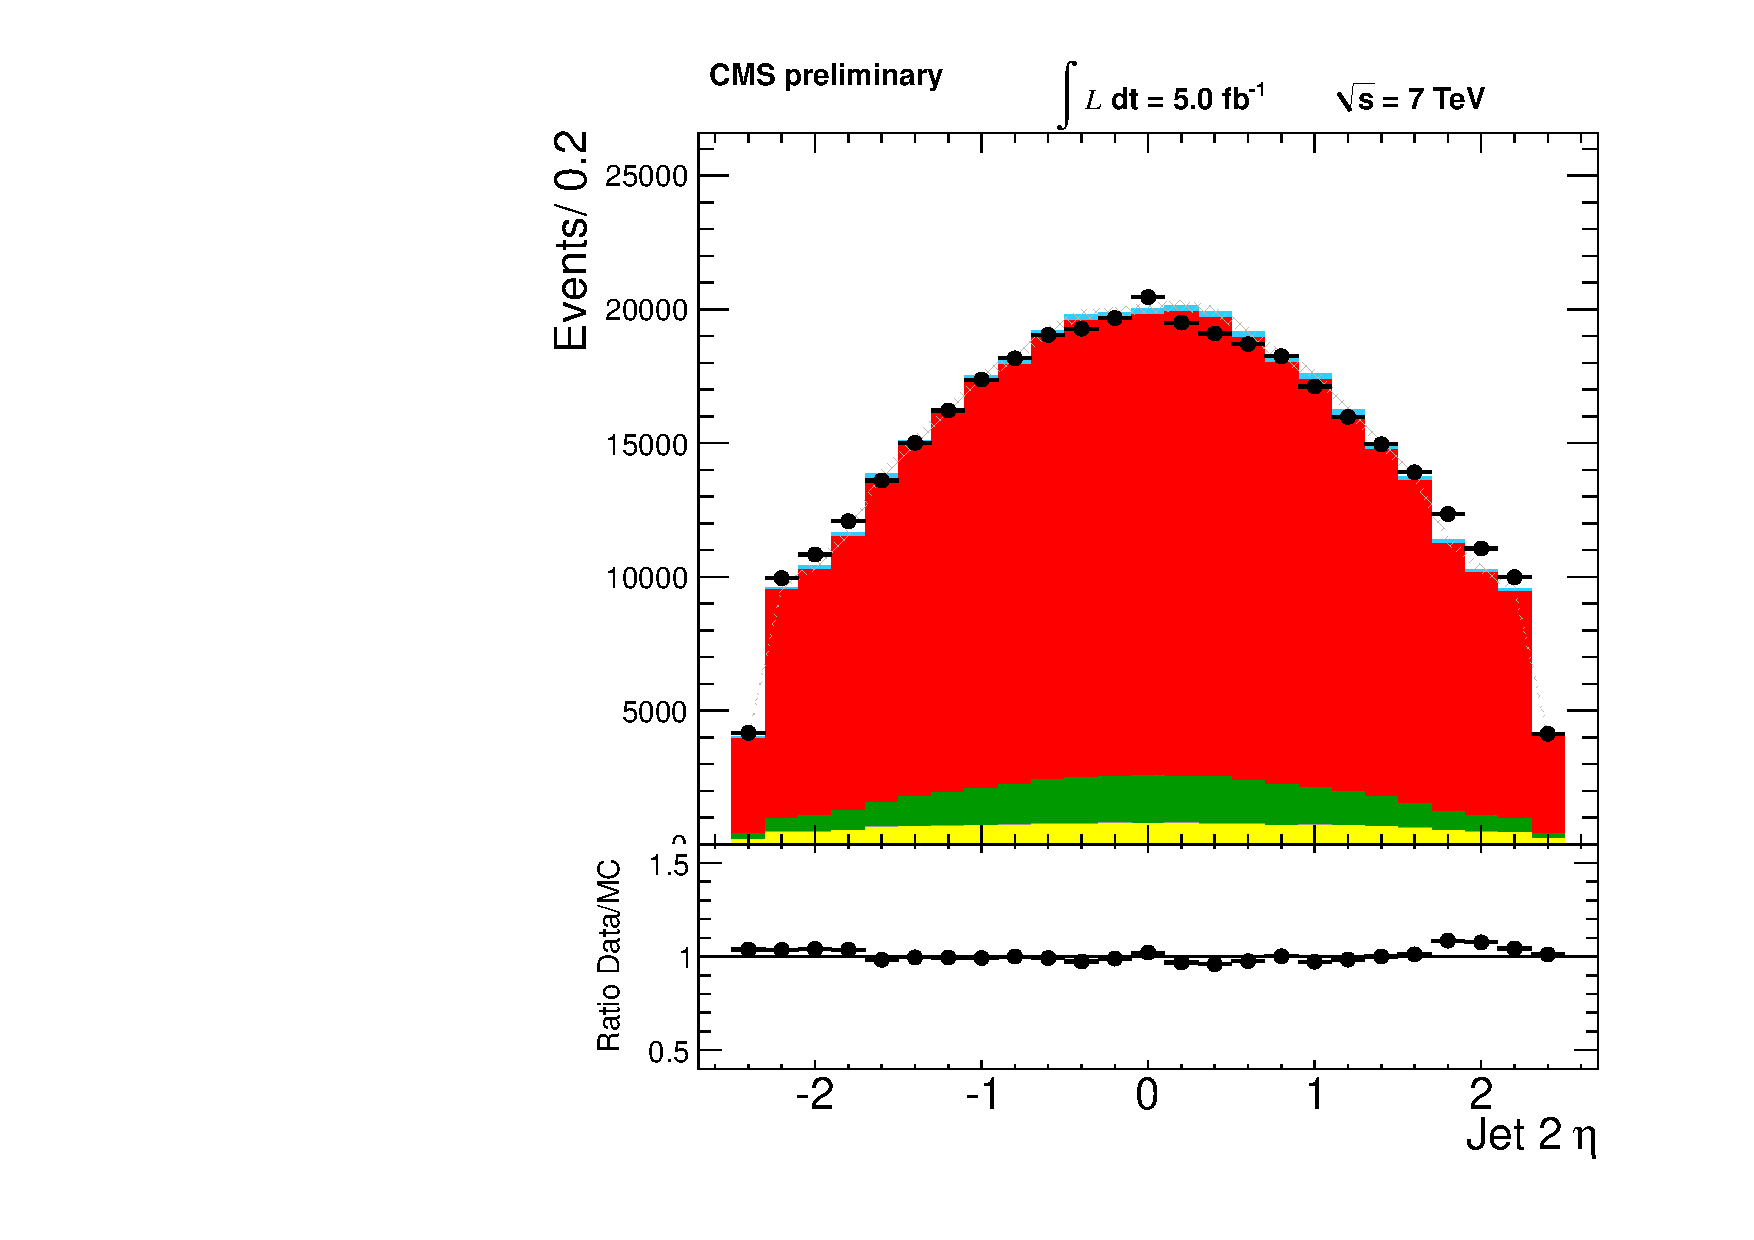
\includegraphics[width=0.49\textwidth]{figs/n-1_plots_mu/mu_jetnt_eta.pdf}
    \caption{Comparison of the leading jet $\eta $ (left) and the
    second leading jet $\eta $ (right) distributions from data and MC
    for the muon+jets selection.  }
\label{fig:mu_jet_eta}}
\end{figure}
%%%%%%%%%%%%%%%%%%%%%%%%%%%%
\begin{figure}[h!t]
  {\centering
    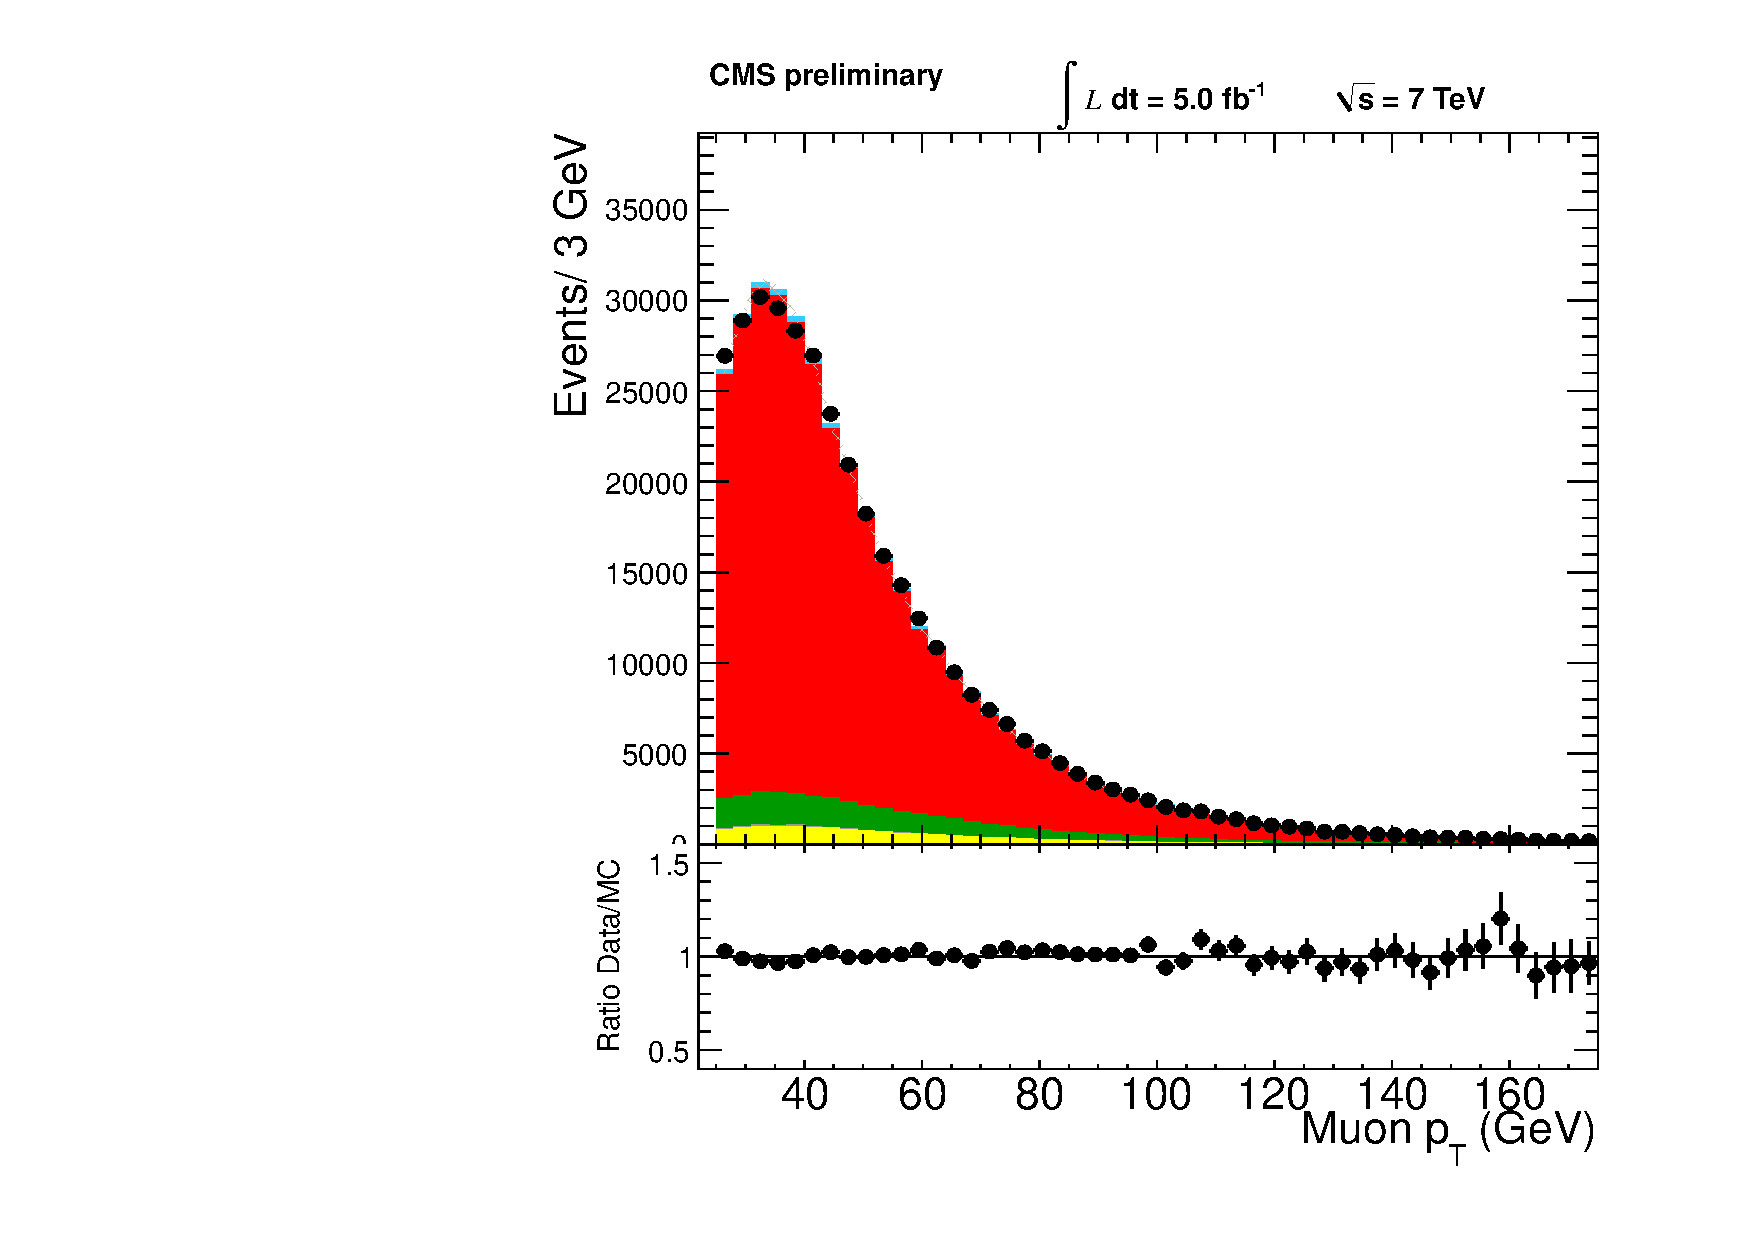
\includegraphics[width=0.49\textwidth]{figs/n-1_plots_mu/mu_W_muon_pt.pdf}
    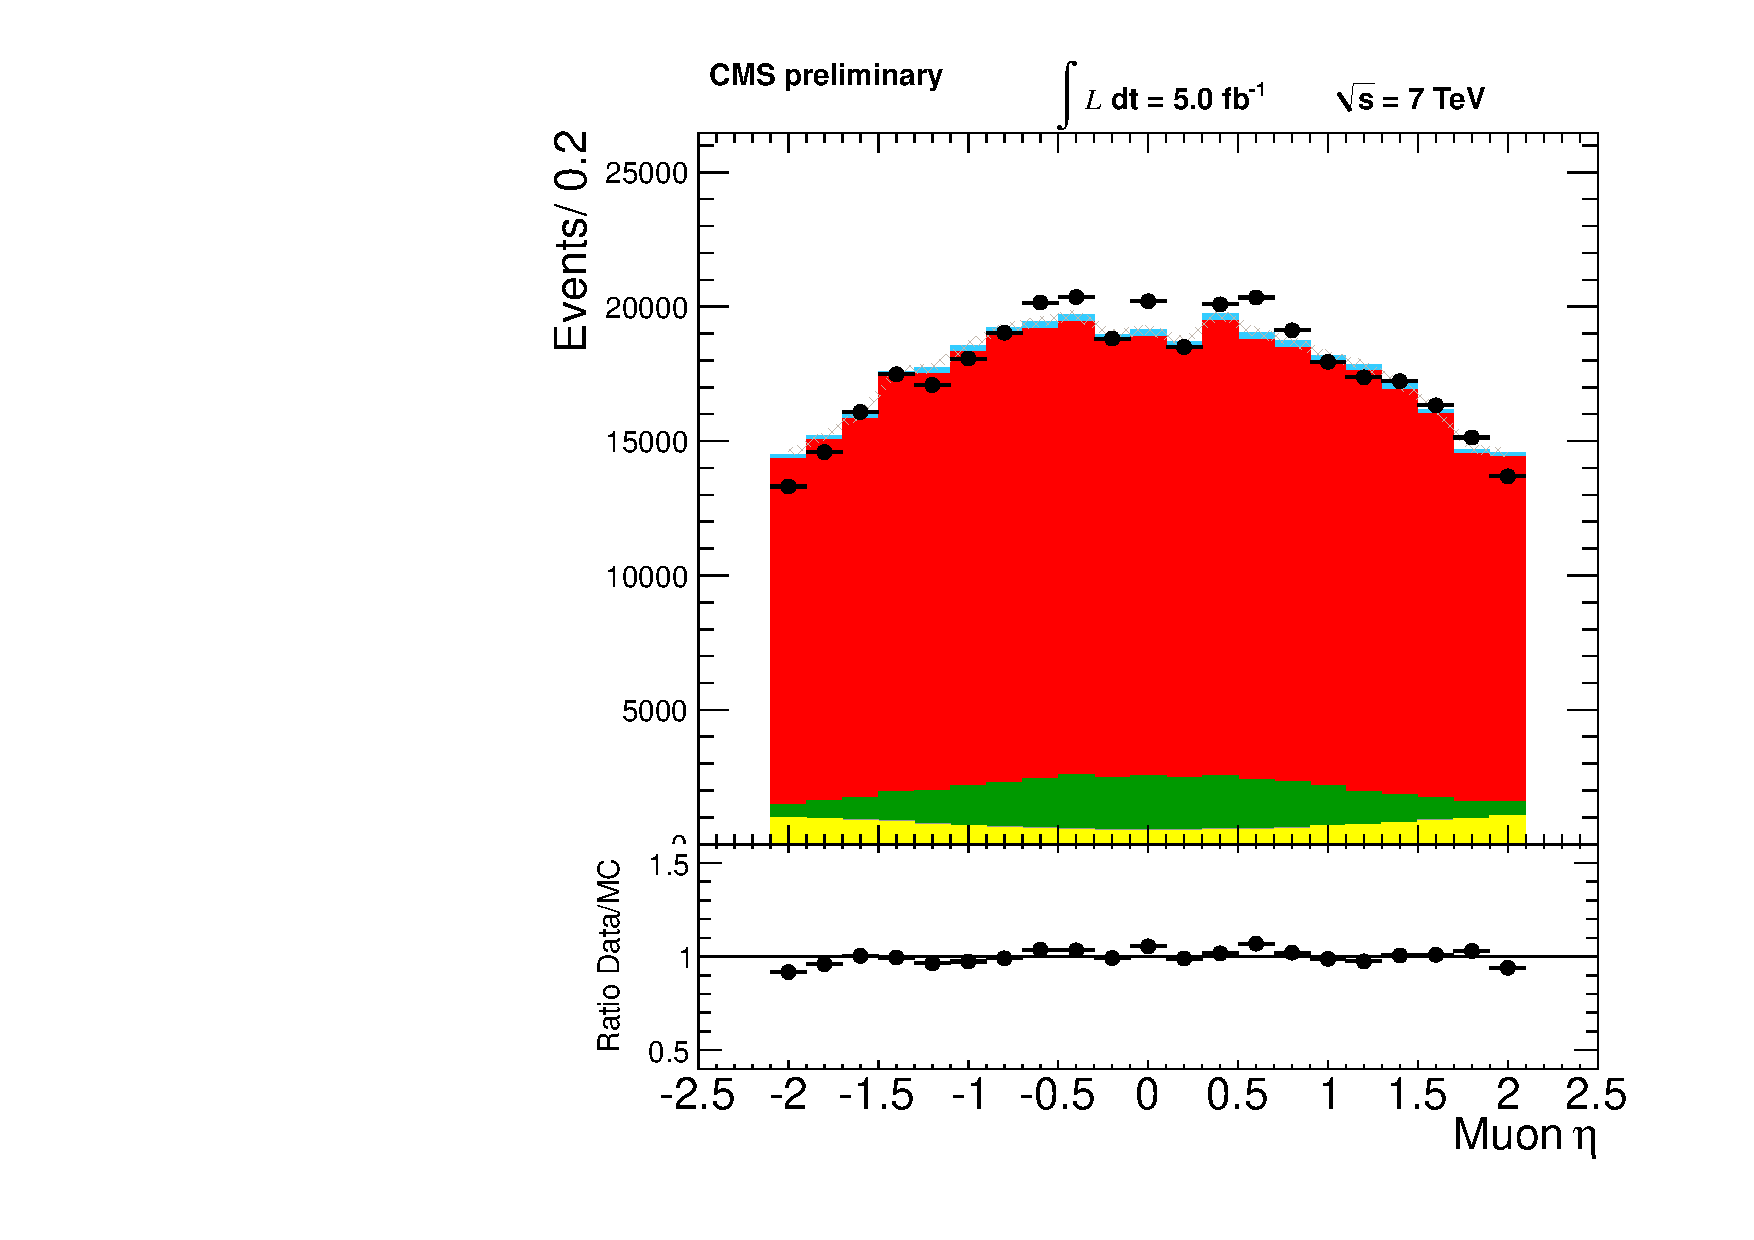
\includegraphics[width=0.49\textwidth]{figs/n-1_plots_mu/mu_W_muon_eta.pdf}
    \caption{Comparison of the muon $p_{T} $ (left) and the
    muon $\eta $ (right) distributions from data and MC for the
    muon+jets selection. 
    }
   \label{fig:mu_muon}}
\end{figure}

%%%%%%%%%%%%%%%%%%%%%%%%%%%%
\begin{figure}[h!t]
  {\centering
    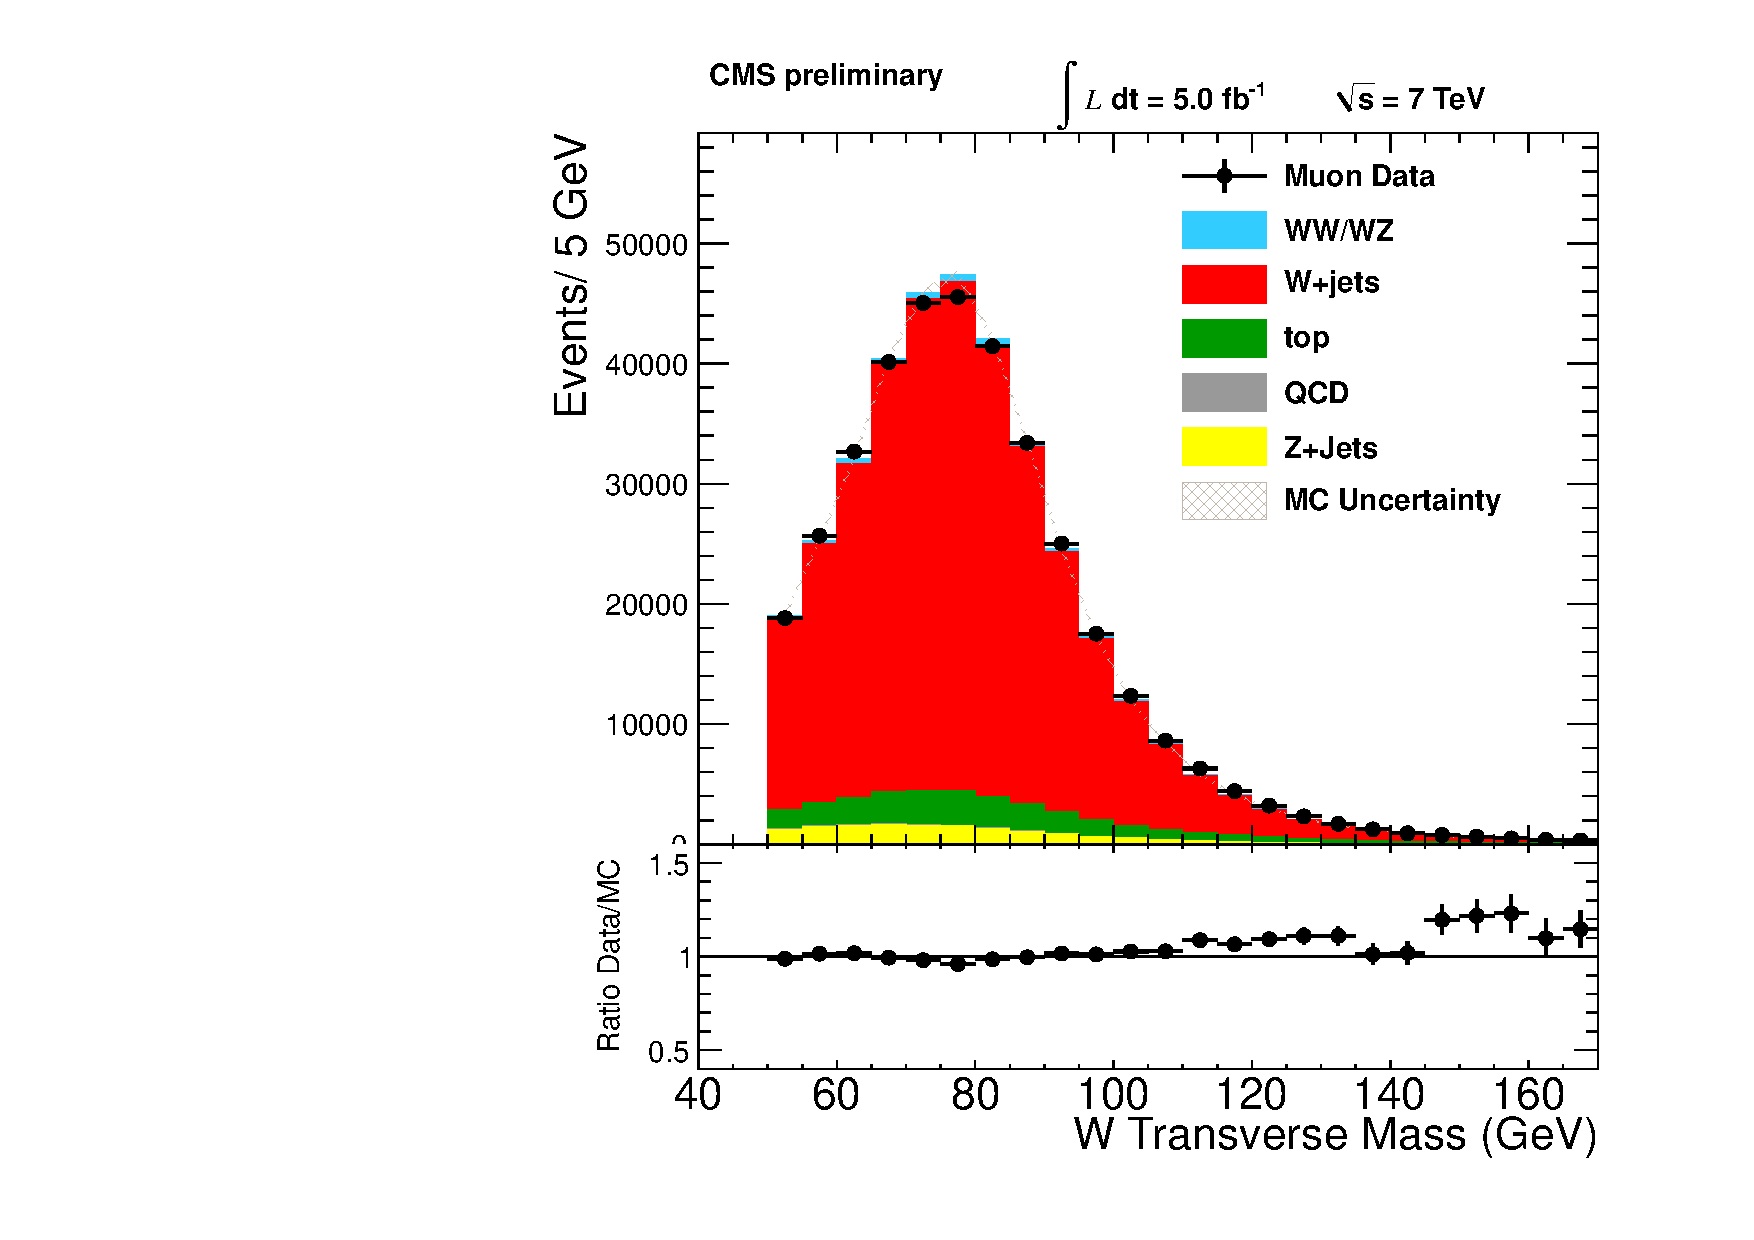
\includegraphics[width=0.49\textwidth]{figs/n-1_plots_mu/mu_W_mt.pdf}
    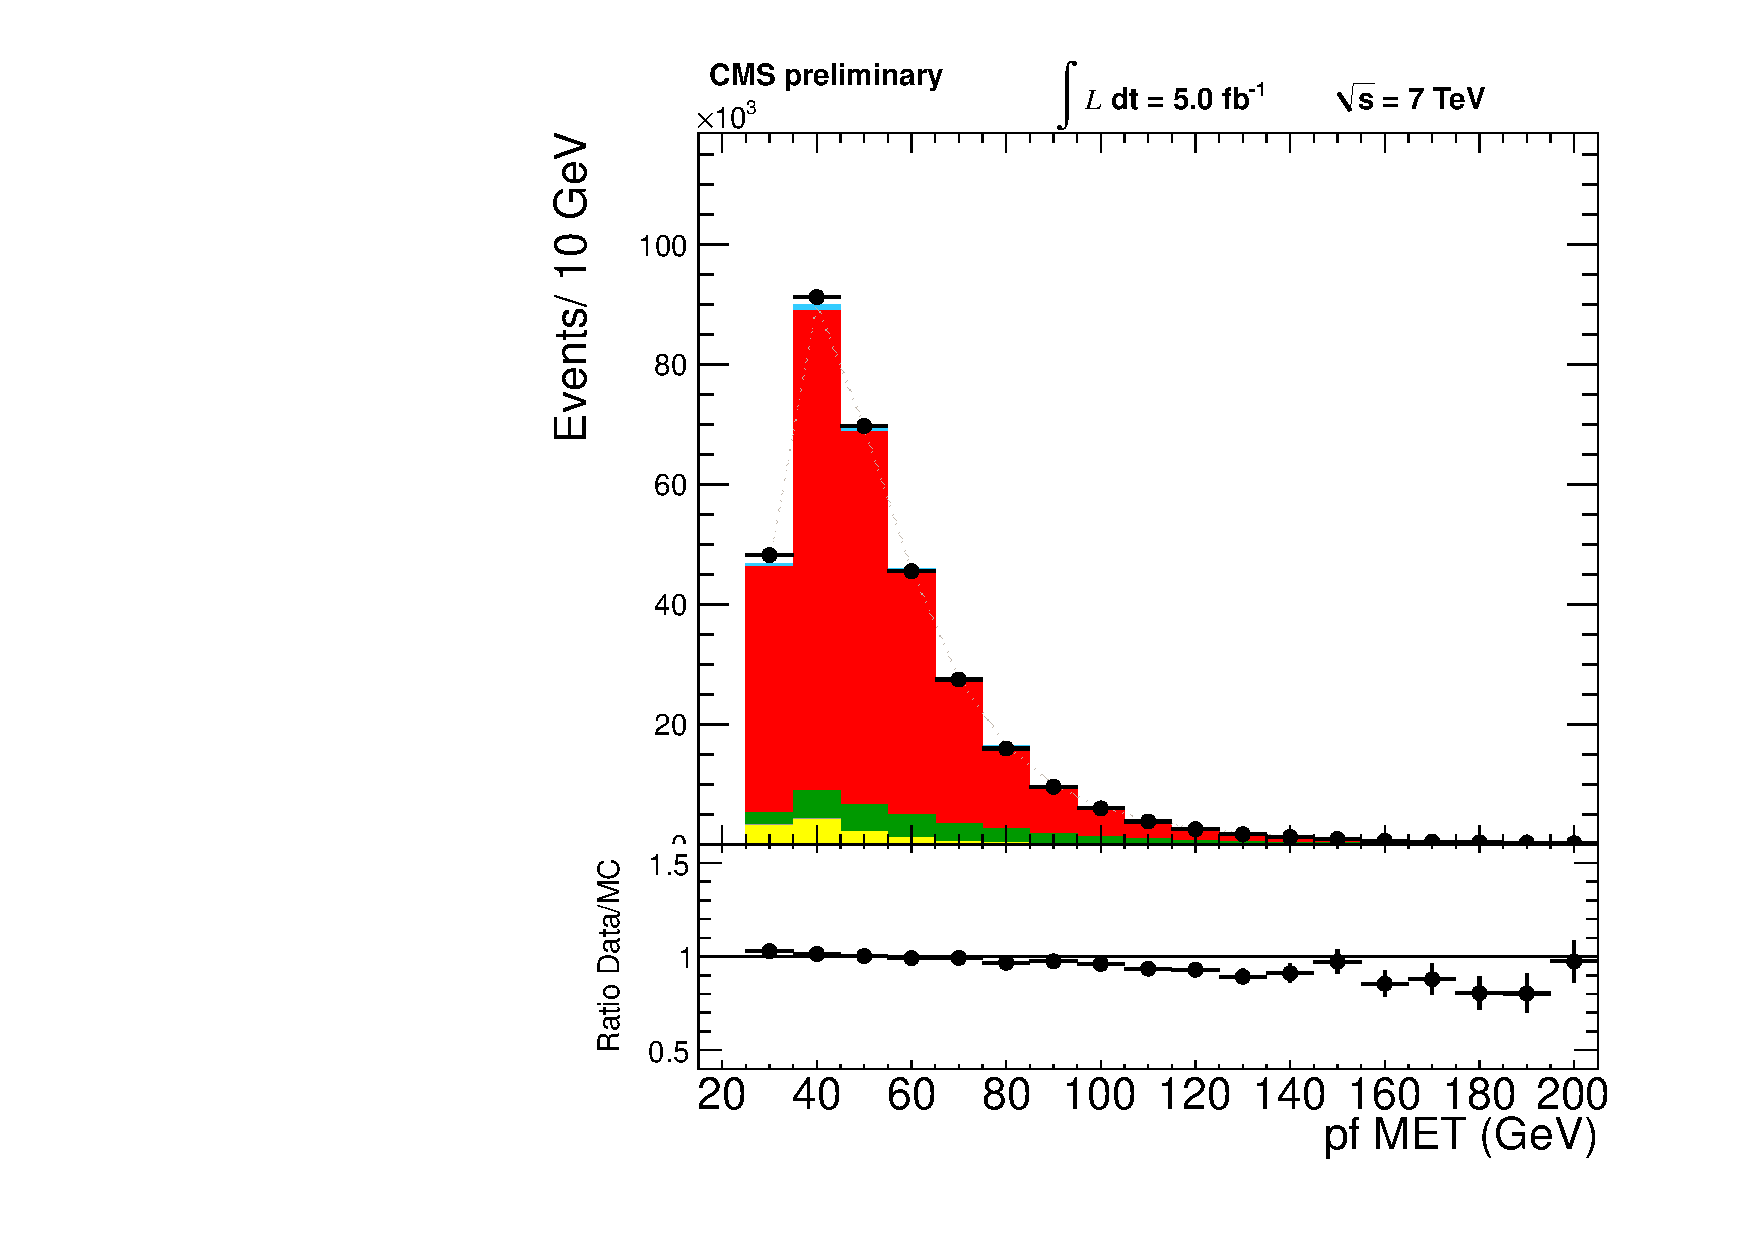
\includegraphics[width=0.49\textwidth]{figs/n-1_plots_mu/mu_event_met_pfmet.pdf}
    \caption{Comparison of the distributions from data and MC of the
     transverse mass of the muon / MET system (left) and the MET (right)
    for the muon+jets selection.
    }
    \label{fig:mu_W_Mt}}
\end{figure}
%%%%%%%%%%%%%%%%%%%%%%%%%%%%
\begin{figure}[h!t]
  {\centering
    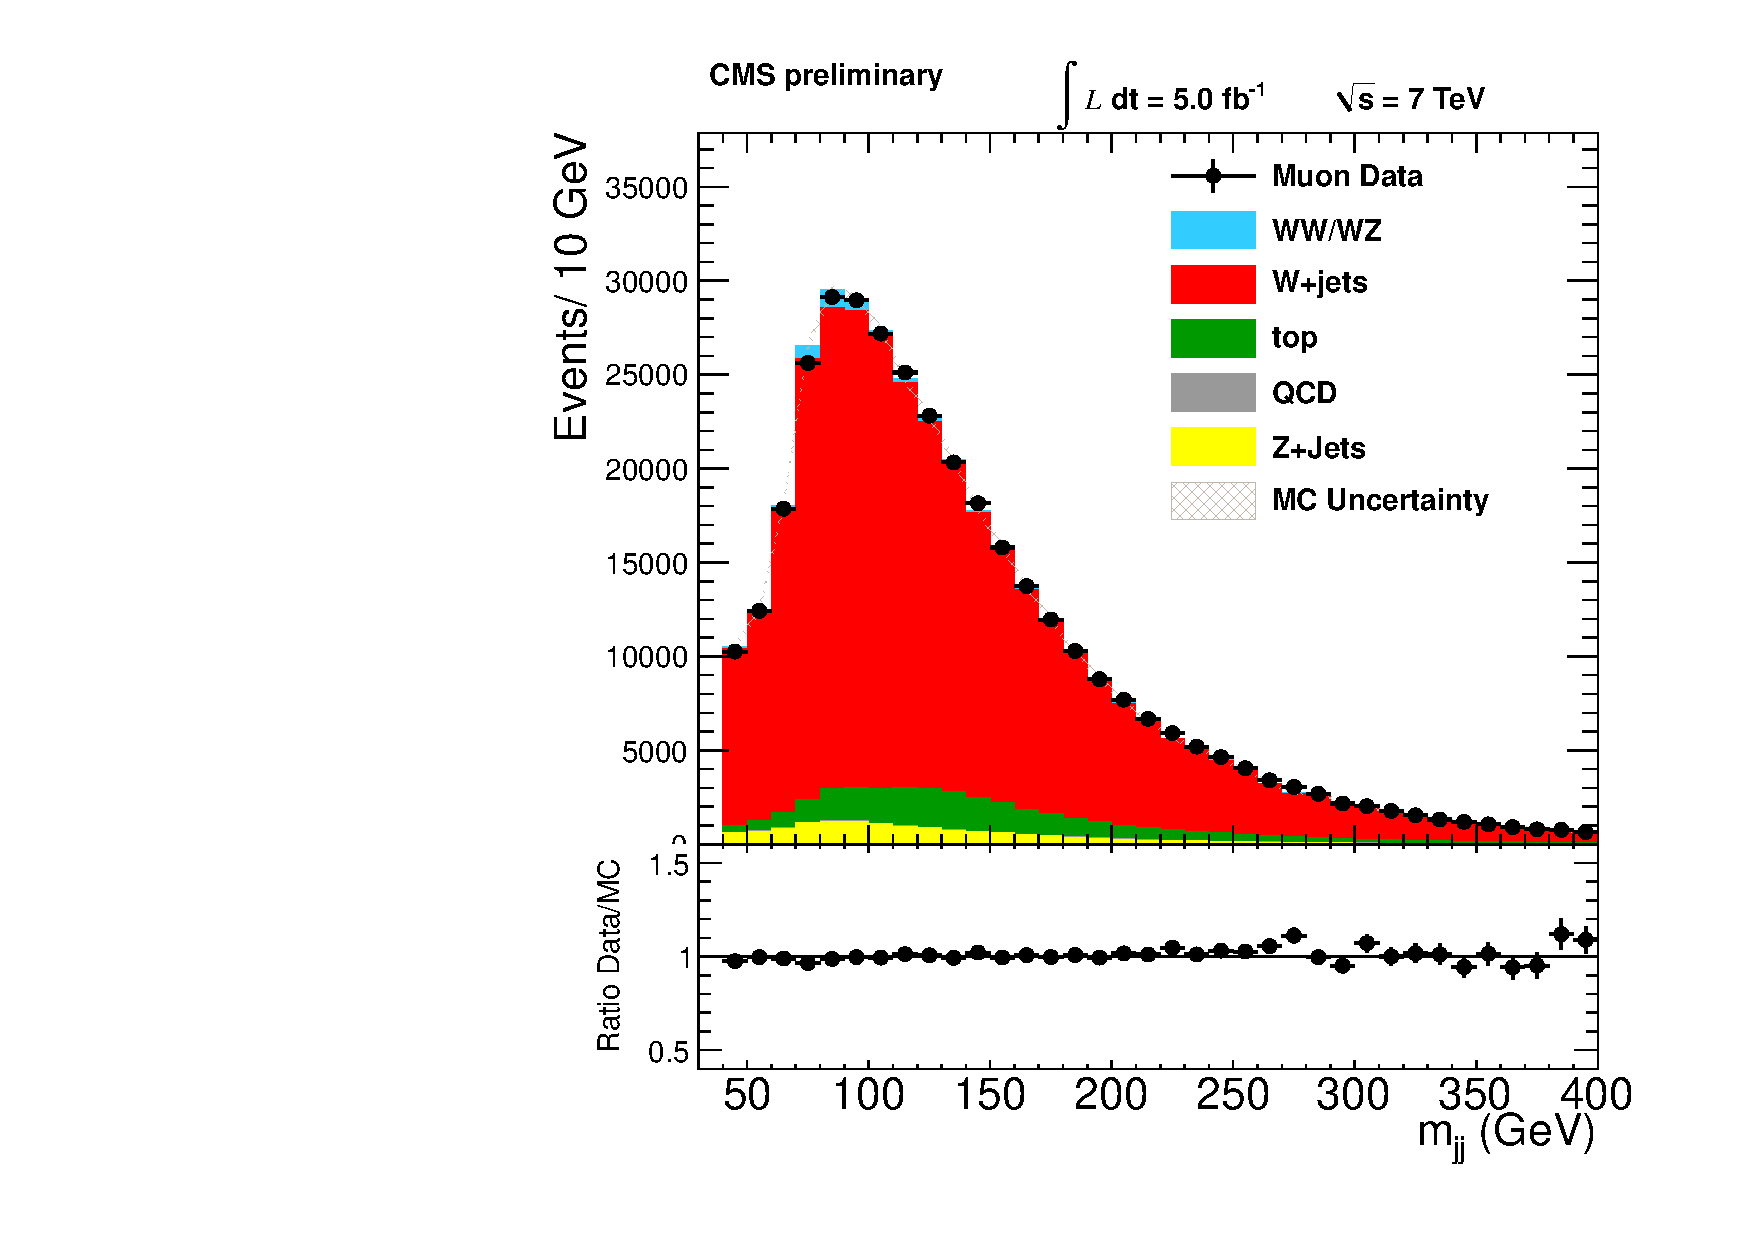
\includegraphics[width=0.49\textwidth]{figs/n-1_plots_mu/mu_mjj.pdf}
    \caption{Comparison of the dijet mass ($m_{JJ}$) distributions from data and MC for 
      the muon+jets selection. }
    \label{fig:mu_mjj}}
\end{figure}

%%%%%%%%%%%%%%%%%%%%%%%%%%%%
%%%%%%%%%%%%%%%%%%%%%%%%%%%%
\begin{figure}[h!t]
  {\centering
    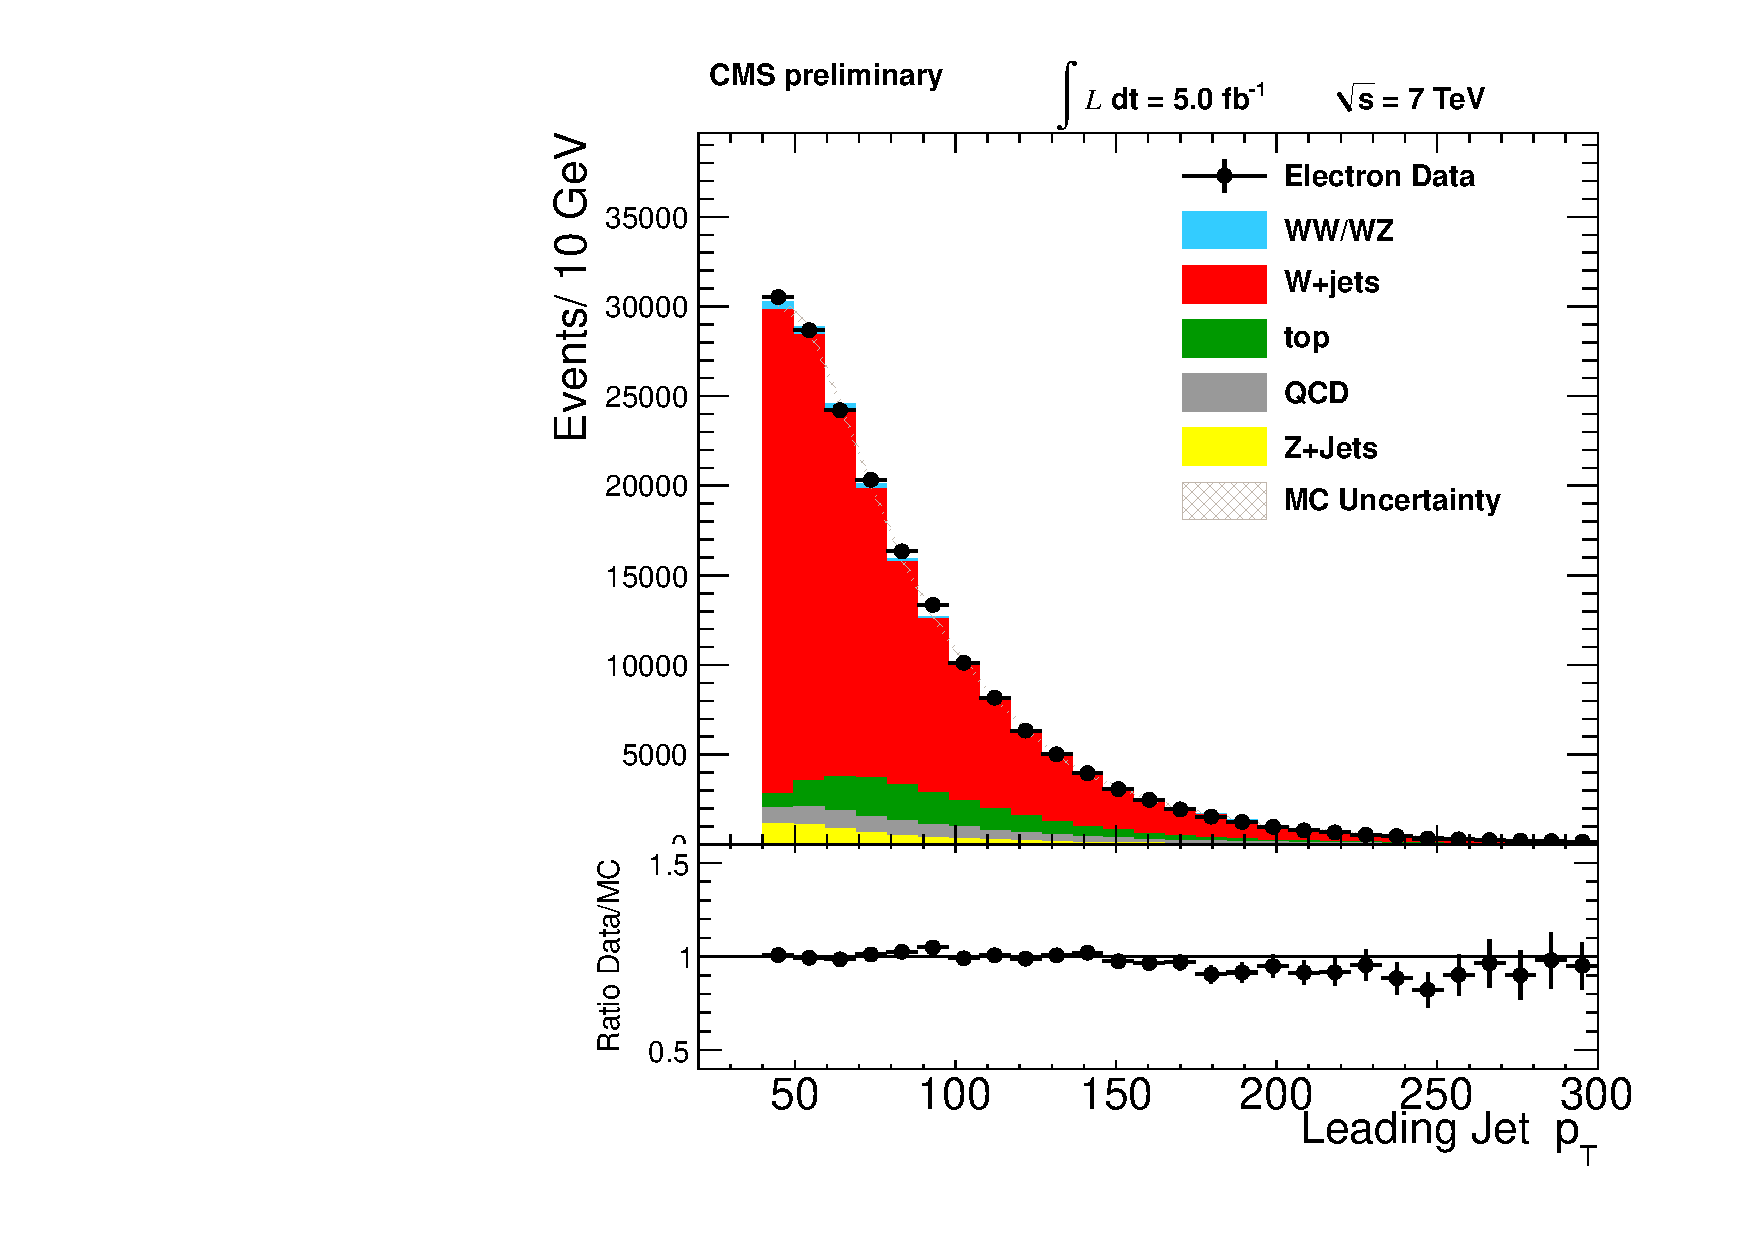
\includegraphics[width=0.49\textwidth]{figs/n-1_plots_el/el_jetld_pt.pdf}
    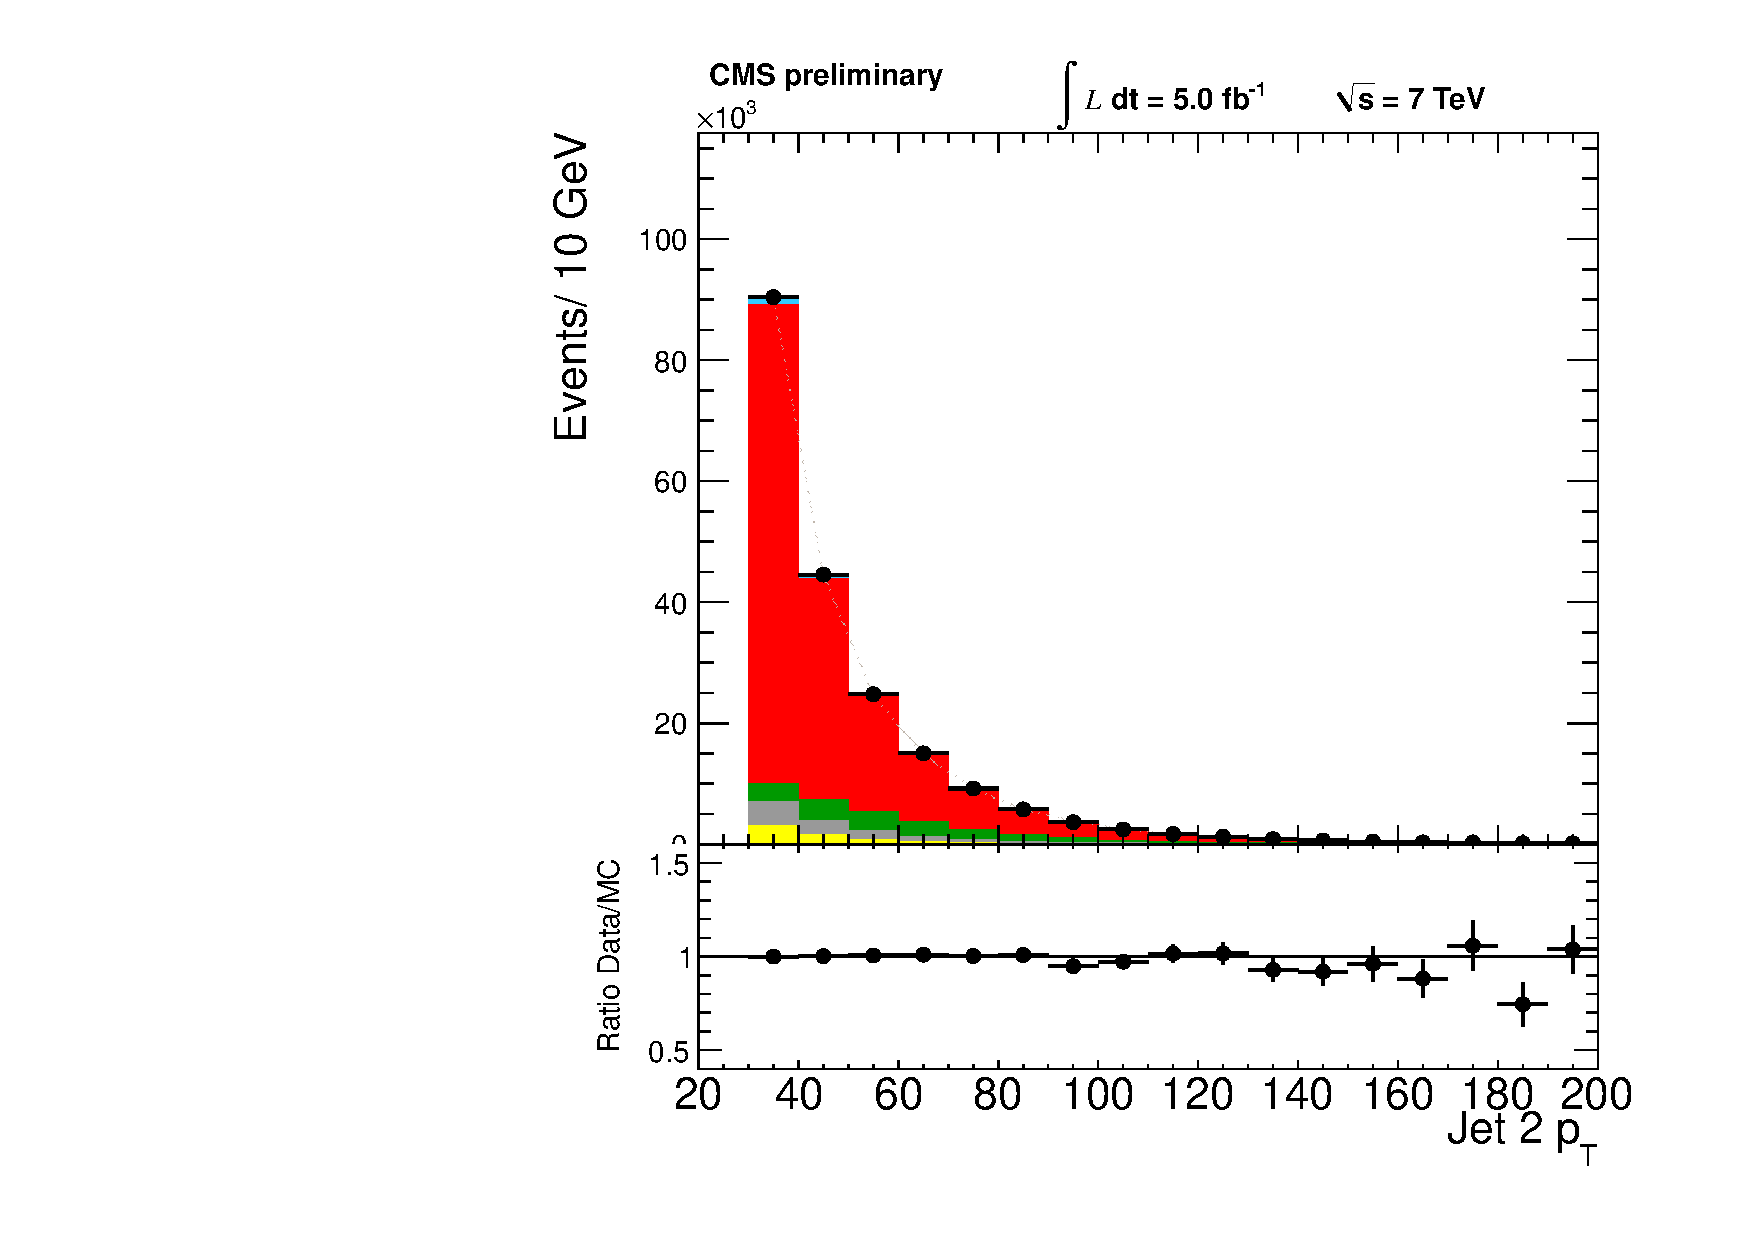
\includegraphics[width=0.49\textwidth]{figs/n-1_plots_el/el_jetnt_pt.pdf}
    \caption{Comparison of the leading jet $p_{T} $ (left) and the
      second leading jet $p_{T} $ (right) distributions from data and MC
      for the electron+jets selection.}
    \label{fig:elec_jet_pt}}
\end{figure}
%%%%%%%%%%%%%%%%%%%%%%%%%%%%
\begin{figure}[h!t]
  {\centering
    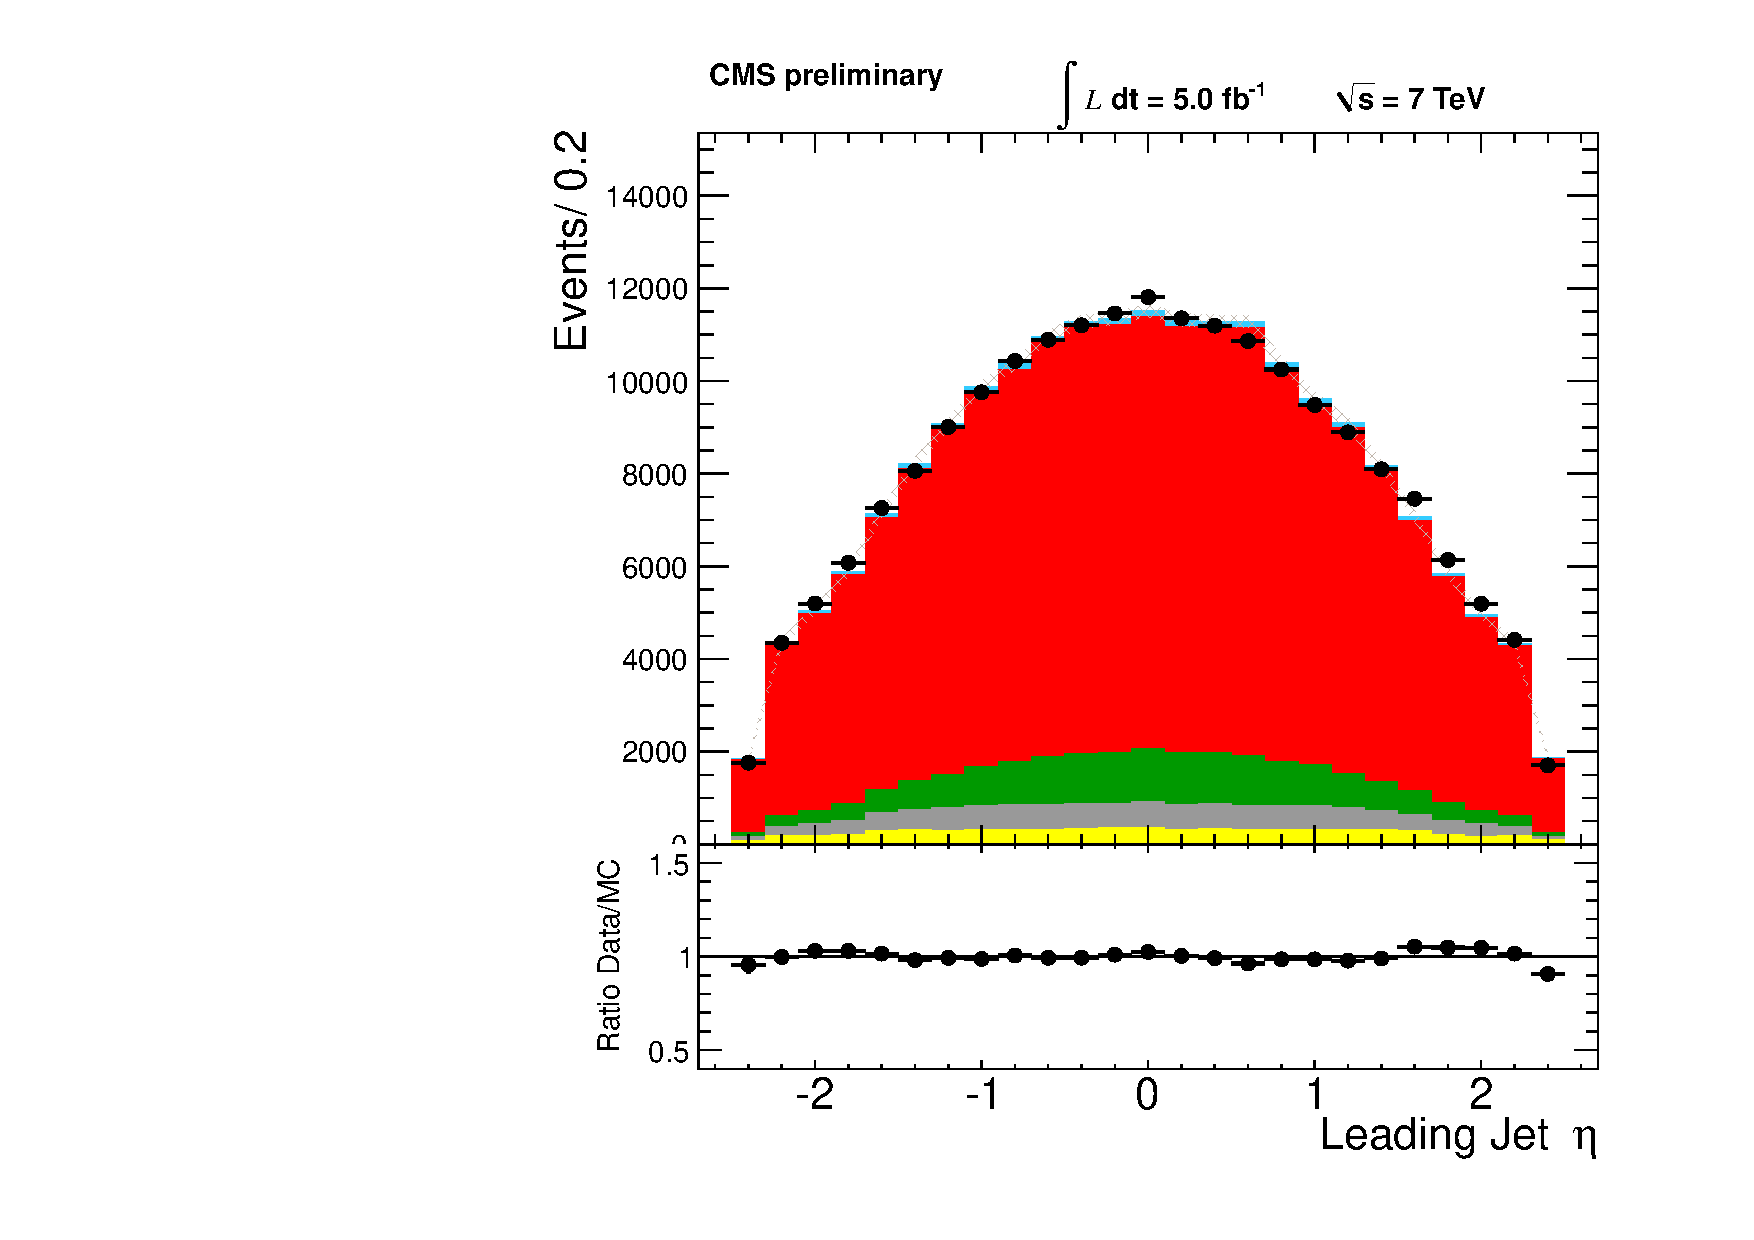
\includegraphics[width=0.49\textwidth]{figs/n-1_plots_el/el_jetld_eta.pdf}
    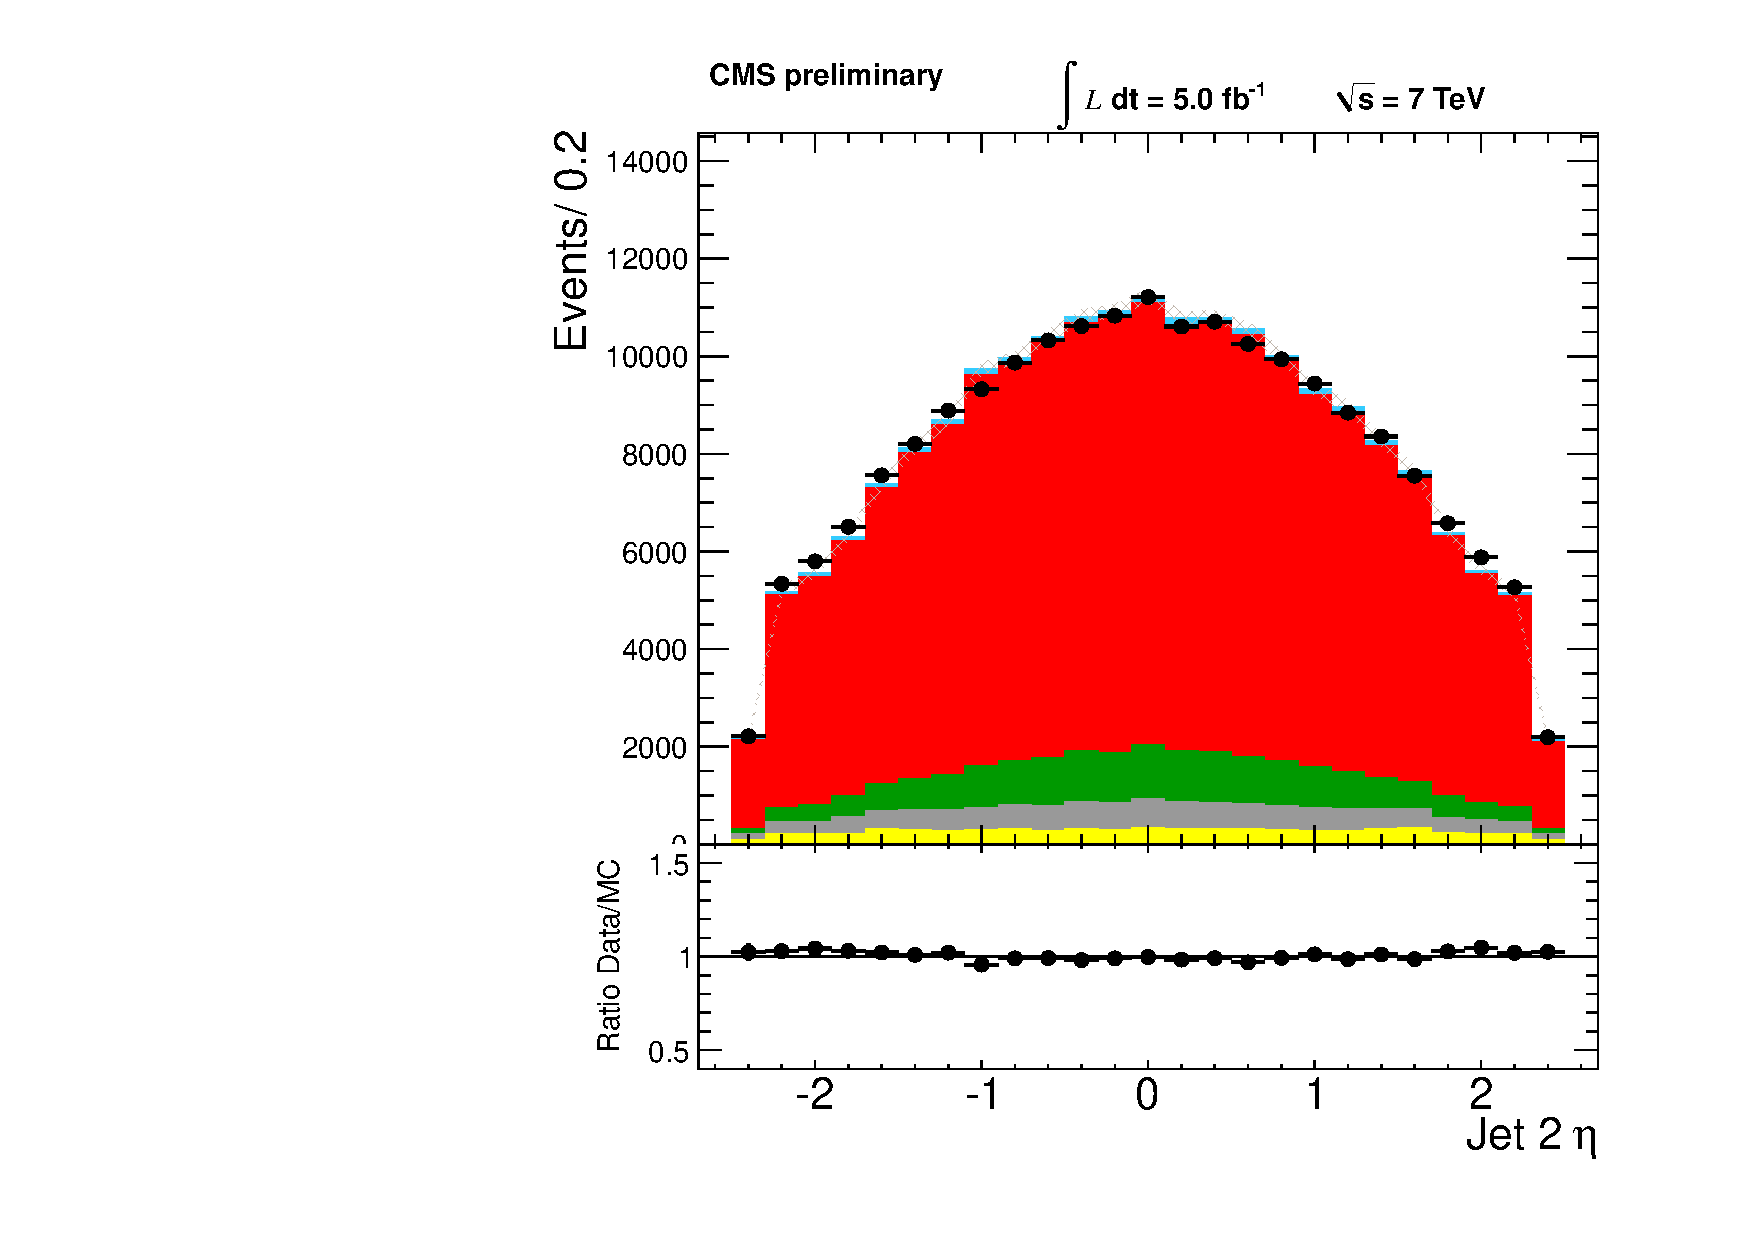
\includegraphics[width=0.49\textwidth]{figs/n-1_plots_el/el_jetnt_eta.pdf}
    \caption{Comparison of the leading jet $\eta $ (left) and the
      second leading jet $\eta $ (right) distributions from data and MC for the electron+jets selection.}
    \label{fig:elec_jet_eta}}
\end{figure}
%%%%%%%%%%%%%%%%%%%%%%%%%%%%
\begin{figure}[h!t]
  {\centering
    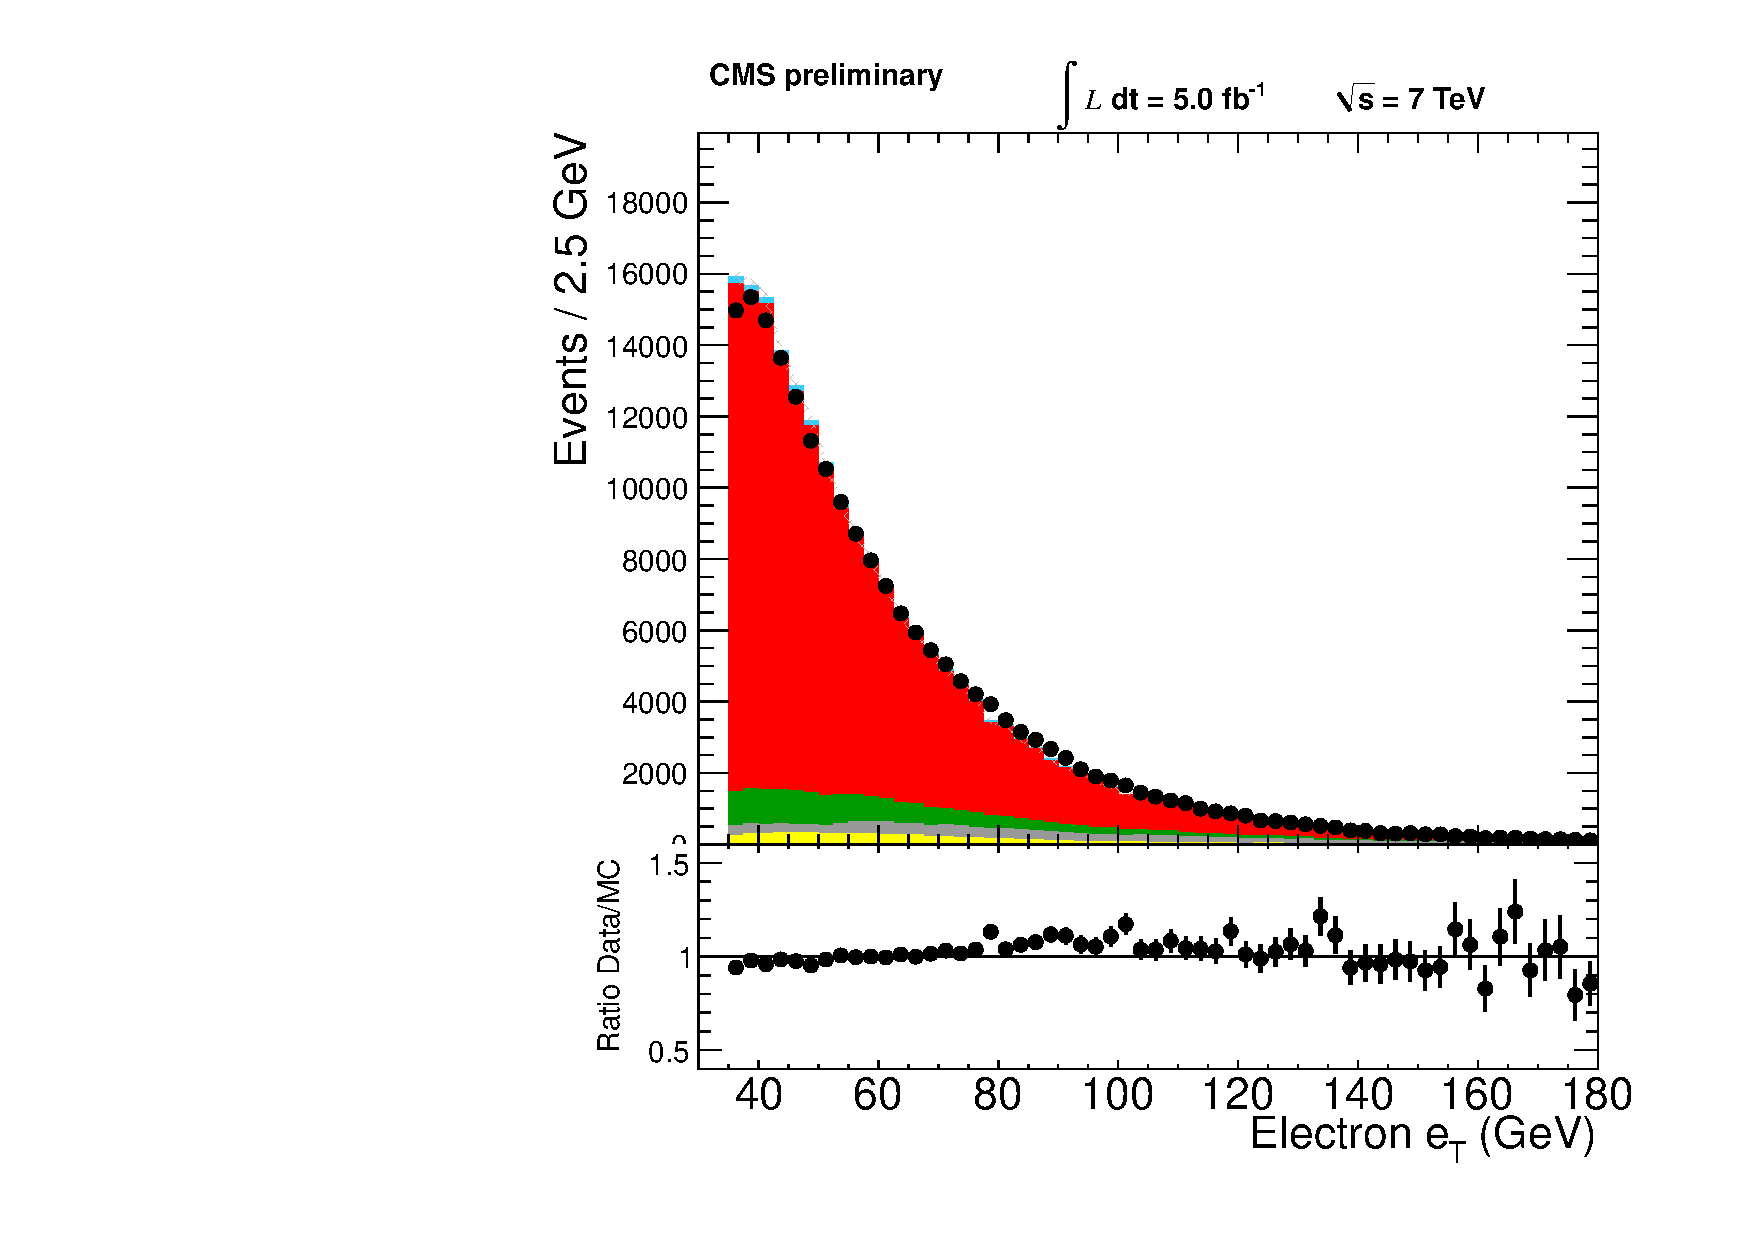
\includegraphics[width=0.49\textwidth]{figs/n-1_plots_el/el_W_electron_et.pdf}
    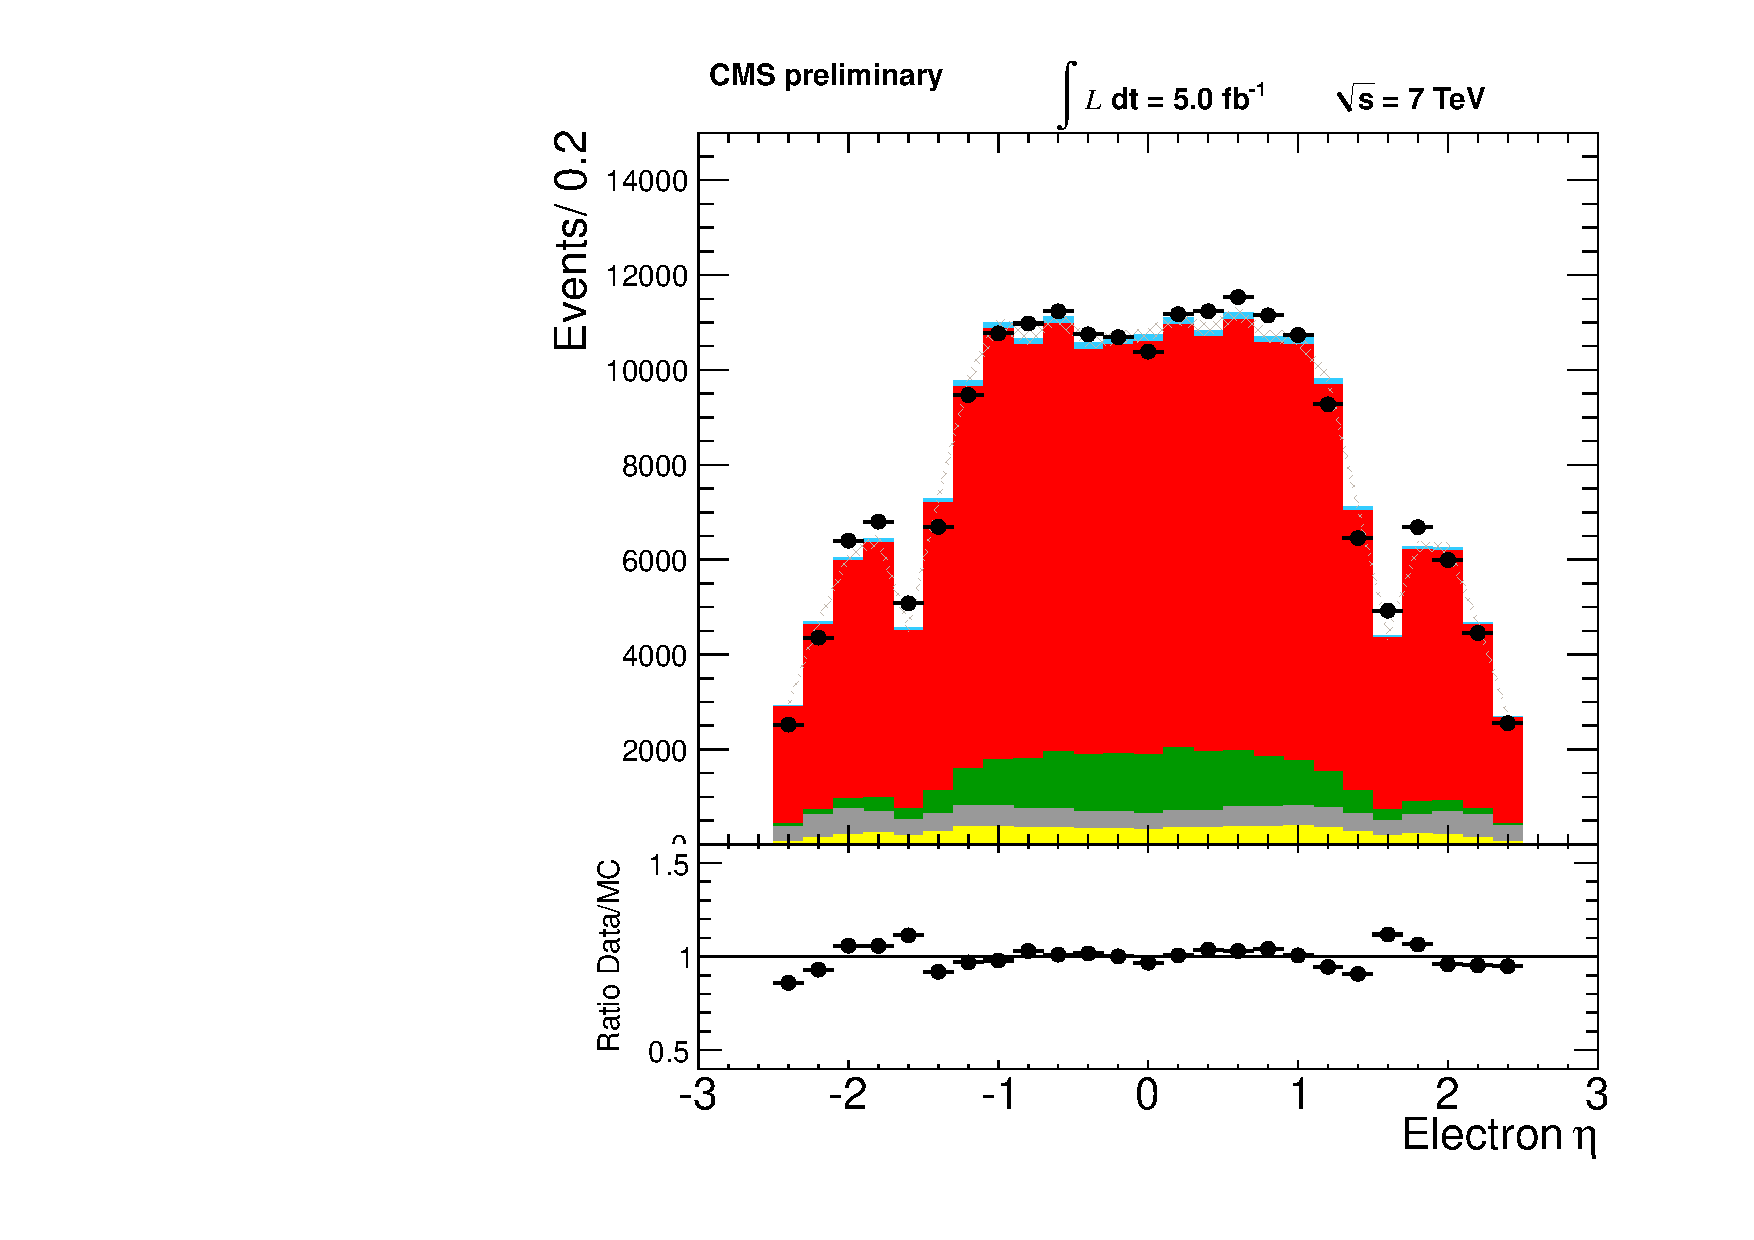
\includegraphics[width=0.49\textwidth]{figs/n-1_plots_el/el_W_electron_eta.pdf}
    \caption{Comparison of the electron $E_{T} $ (left) and the
    electron $\eta $ (right) distributions from data and MC for the
    electron+jets selection. 
    }
   \label{fig:elec_electron}}
\end{figure}
%%%%%%%%%%%%%%%%%%%%%%%%%%%%
\begin{figure}[h!t]
  {\centering
    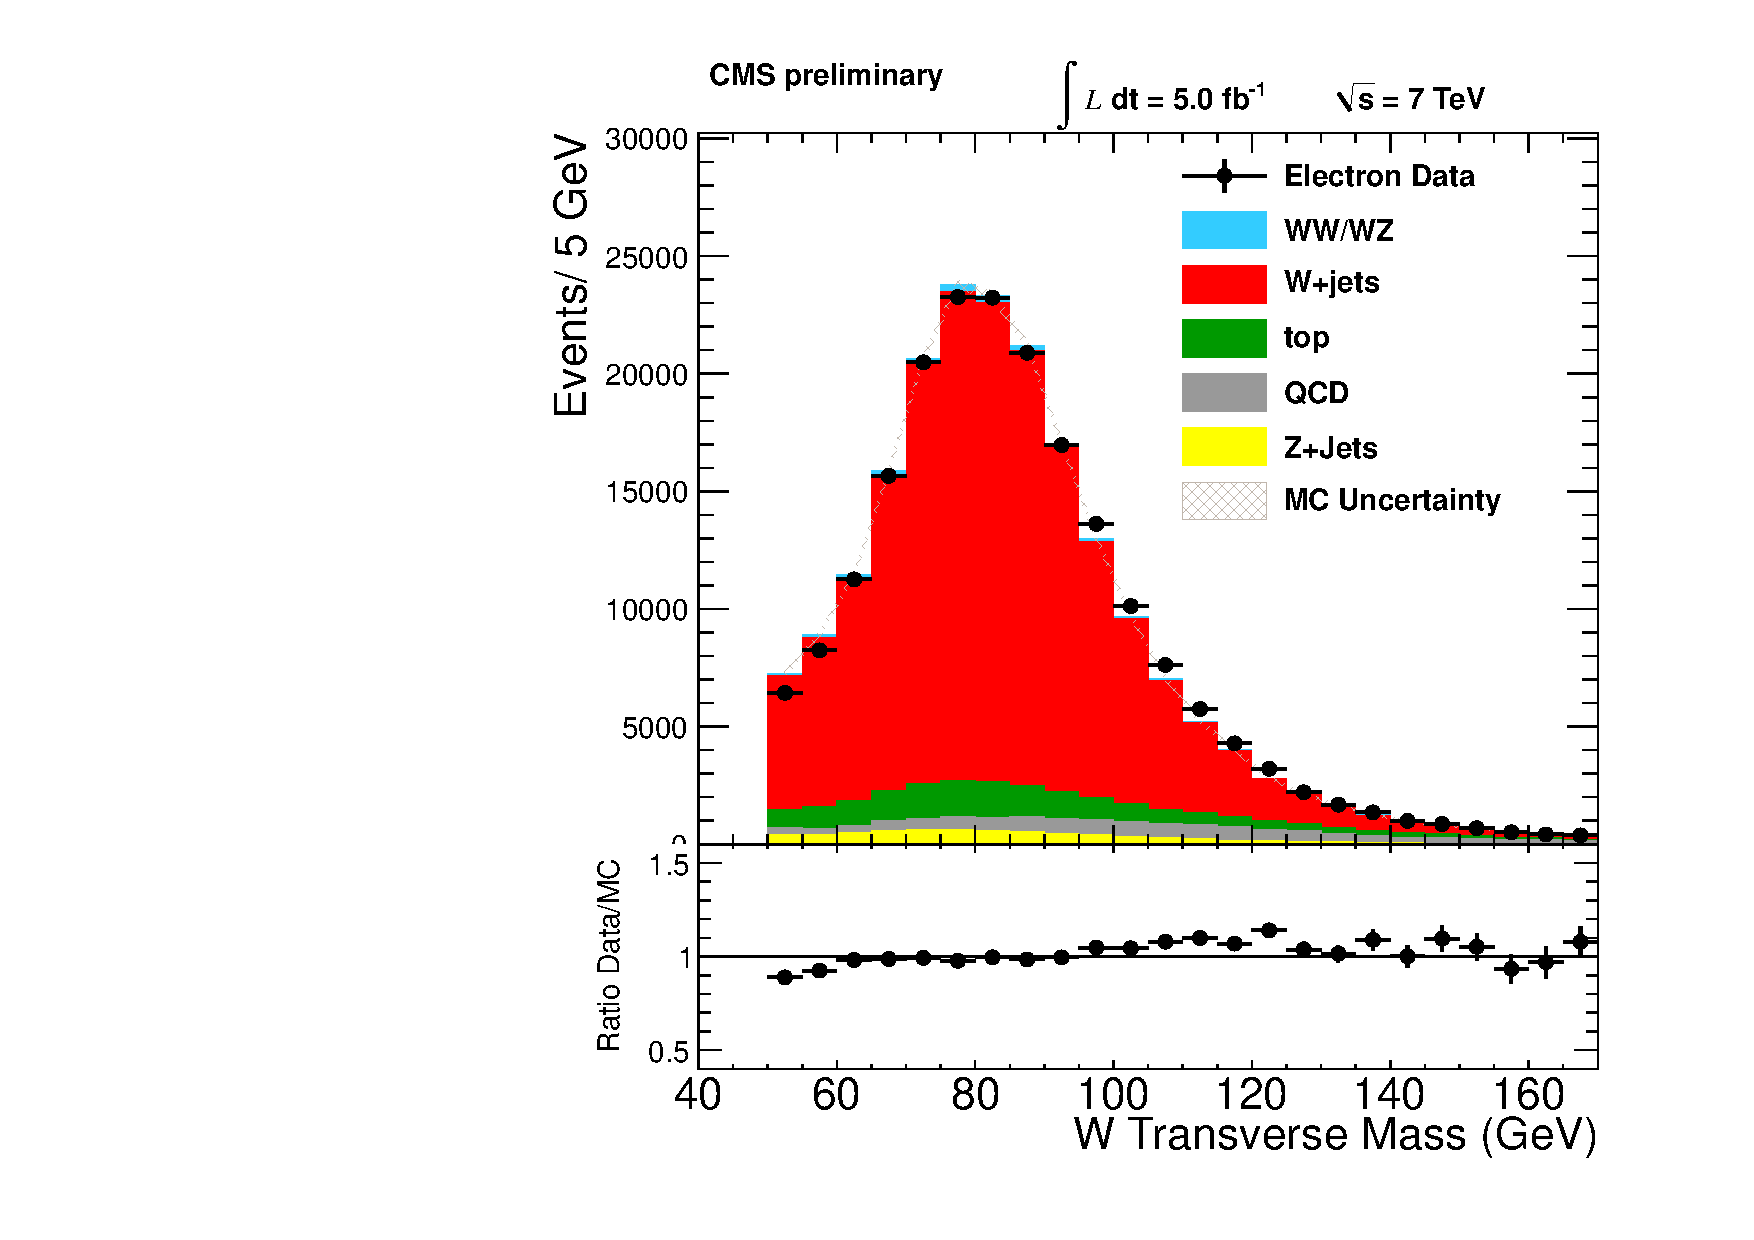
\includegraphics[width=0.49\textwidth]{figs/n-1_plots_el/el_W_mt.pdf}
    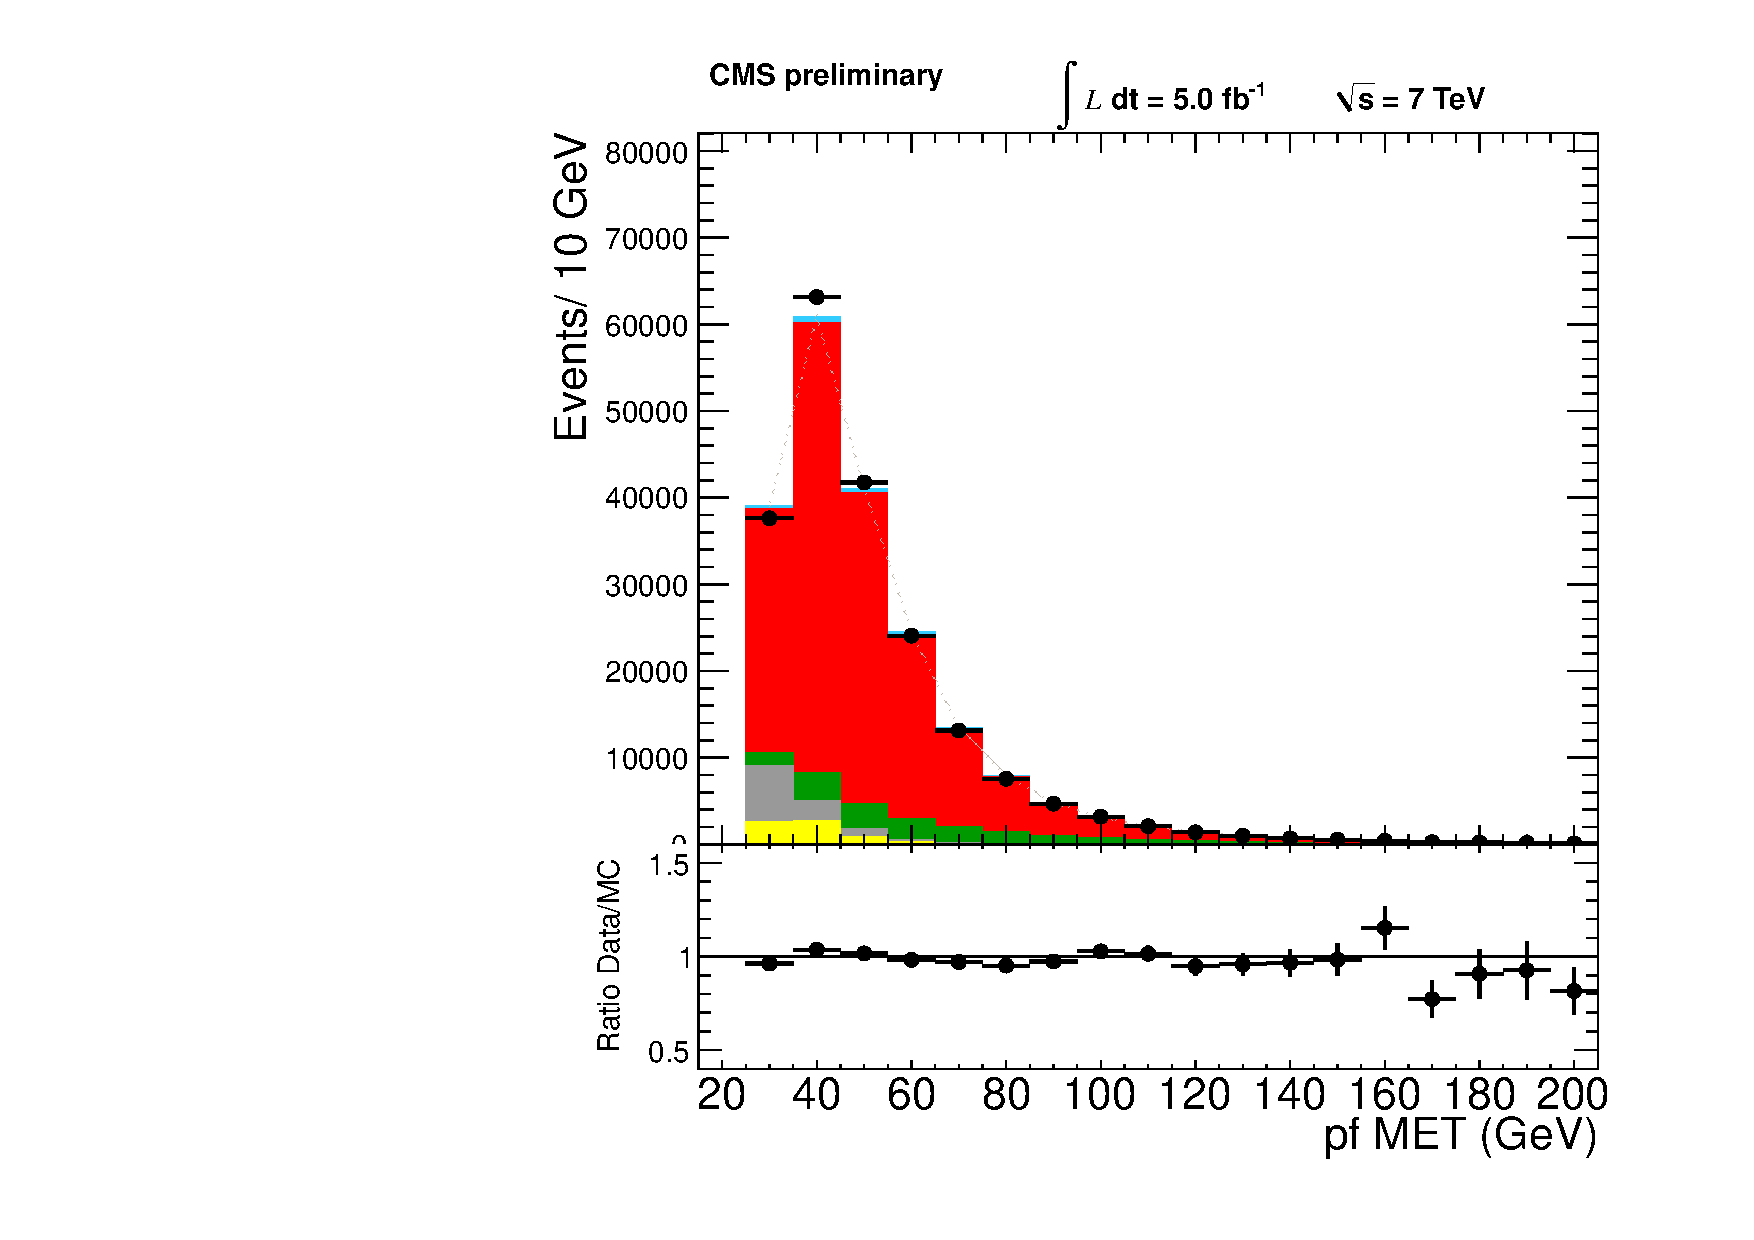
\includegraphics[width=0.49\textwidth]{figs/n-1_plots_el/el_event_met_pfmet.pdf}
    \caption{Comparison of the distributions from data and MC of the transverse mass
     of electron / MET system (left) and the MET (right) for the
      electron+jets selection. 
      }
    \label{fig:elec_W_Mt}}
\end{figure}
%%%%%%%%%%%%%%%%%%%%%%%%%%%%
\begin{figure}[h!t]
  {\centering
    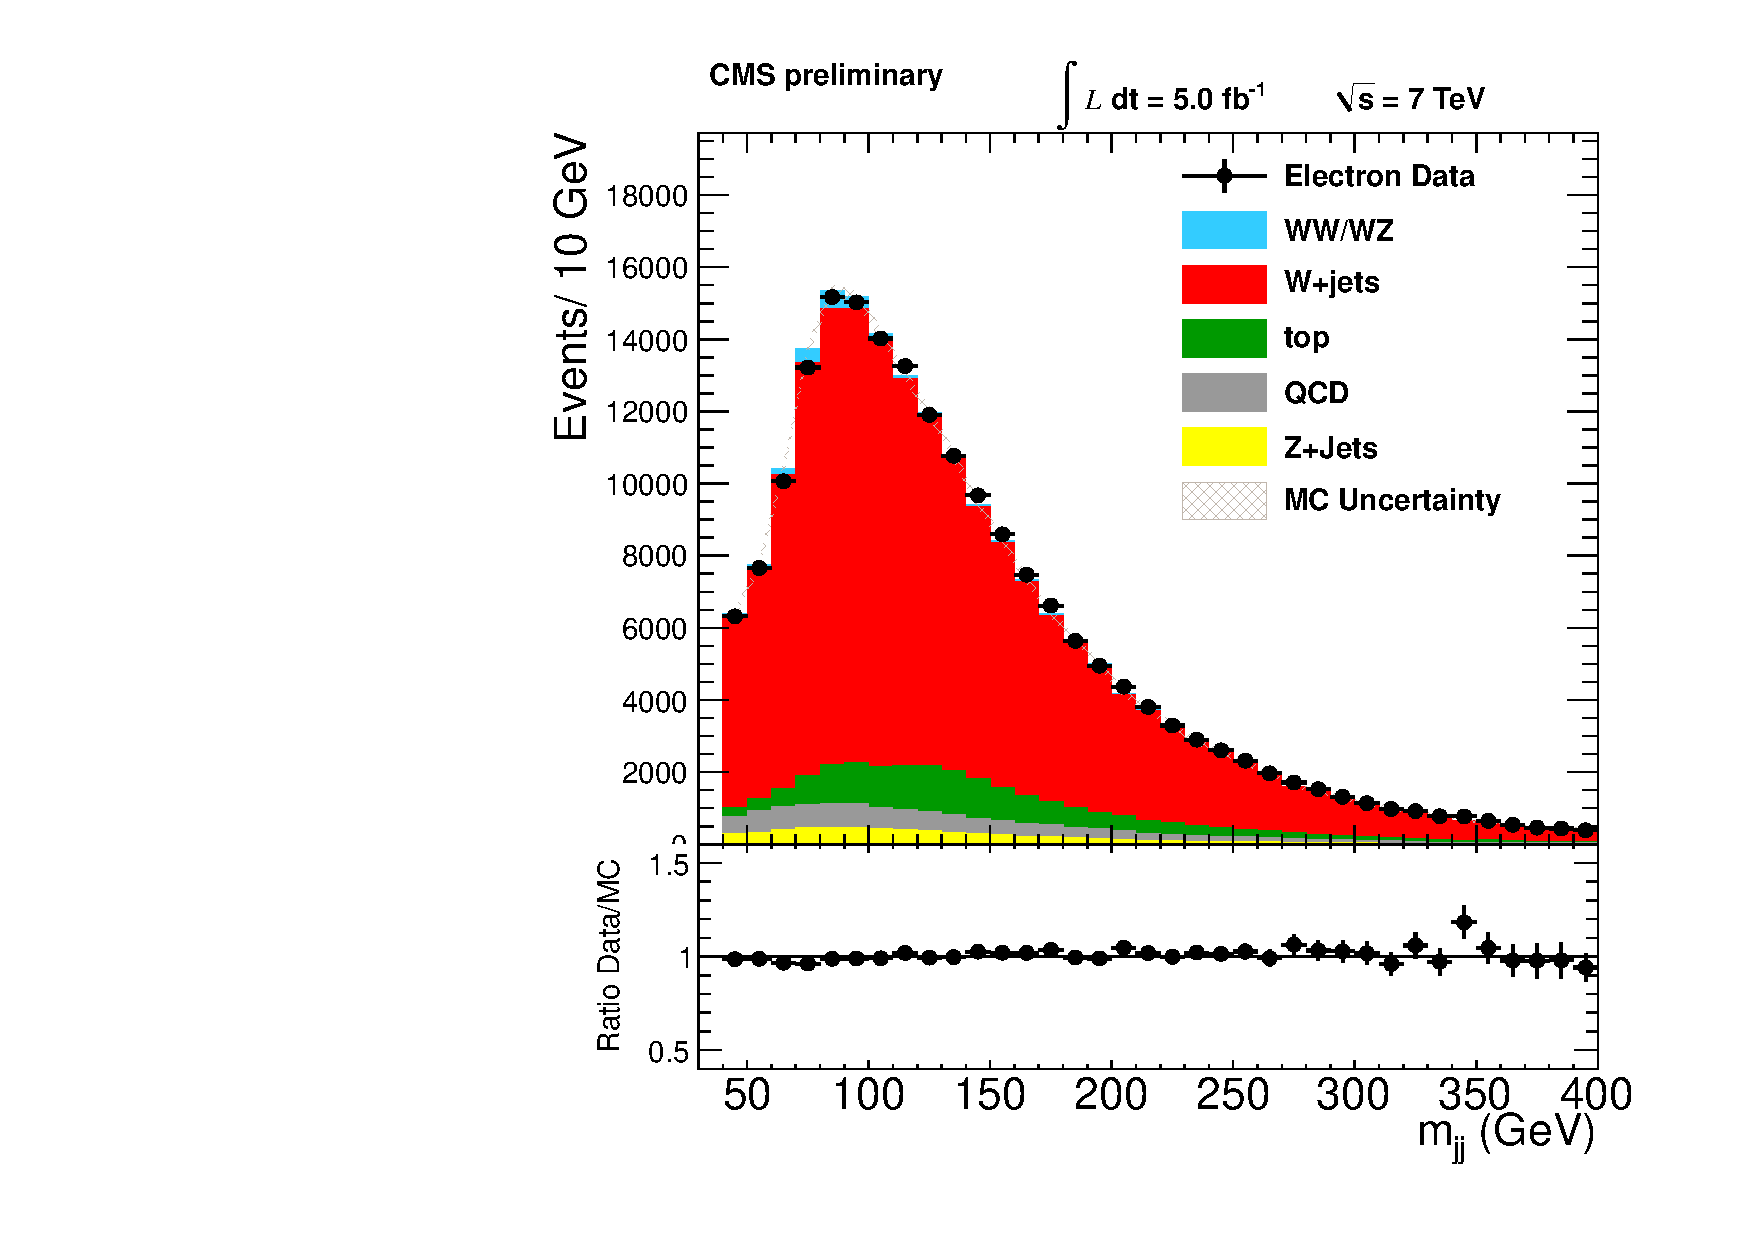
\includegraphics[width=0.49\textwidth]{figs/n-1_plots_el/el_mjj.pdf}
    \caption{Comparison of the dijet mass ($m_{JJ}$) distributions from data and MC for 
      the electron+jets selection. }
    \label{fig:elec_mjj}}
\end{figure}
%%%%%%%%%%%%%%%%%%%%%%%%%%%%
%%%%%%%%%%%%%%%%%%%%%%%%%%%%
\clearpage
The data MC comparison for the various inputs to the MVA are shown in  
Figures ~\ref{fig:mu_jet_qgl}-\ref{fig:mu_ww}
for the muon+jets sample and in 
Figures ~\ref{fig:elec_jet_qgl}-\ref{fig:elec_ww} for
the electron+jets sample. 

% quark-gluon discriminants
%%%%%%%%%%%%%%%%%%%%%%%%%%%%
\begin{figure}[h!t]
  {\centering
    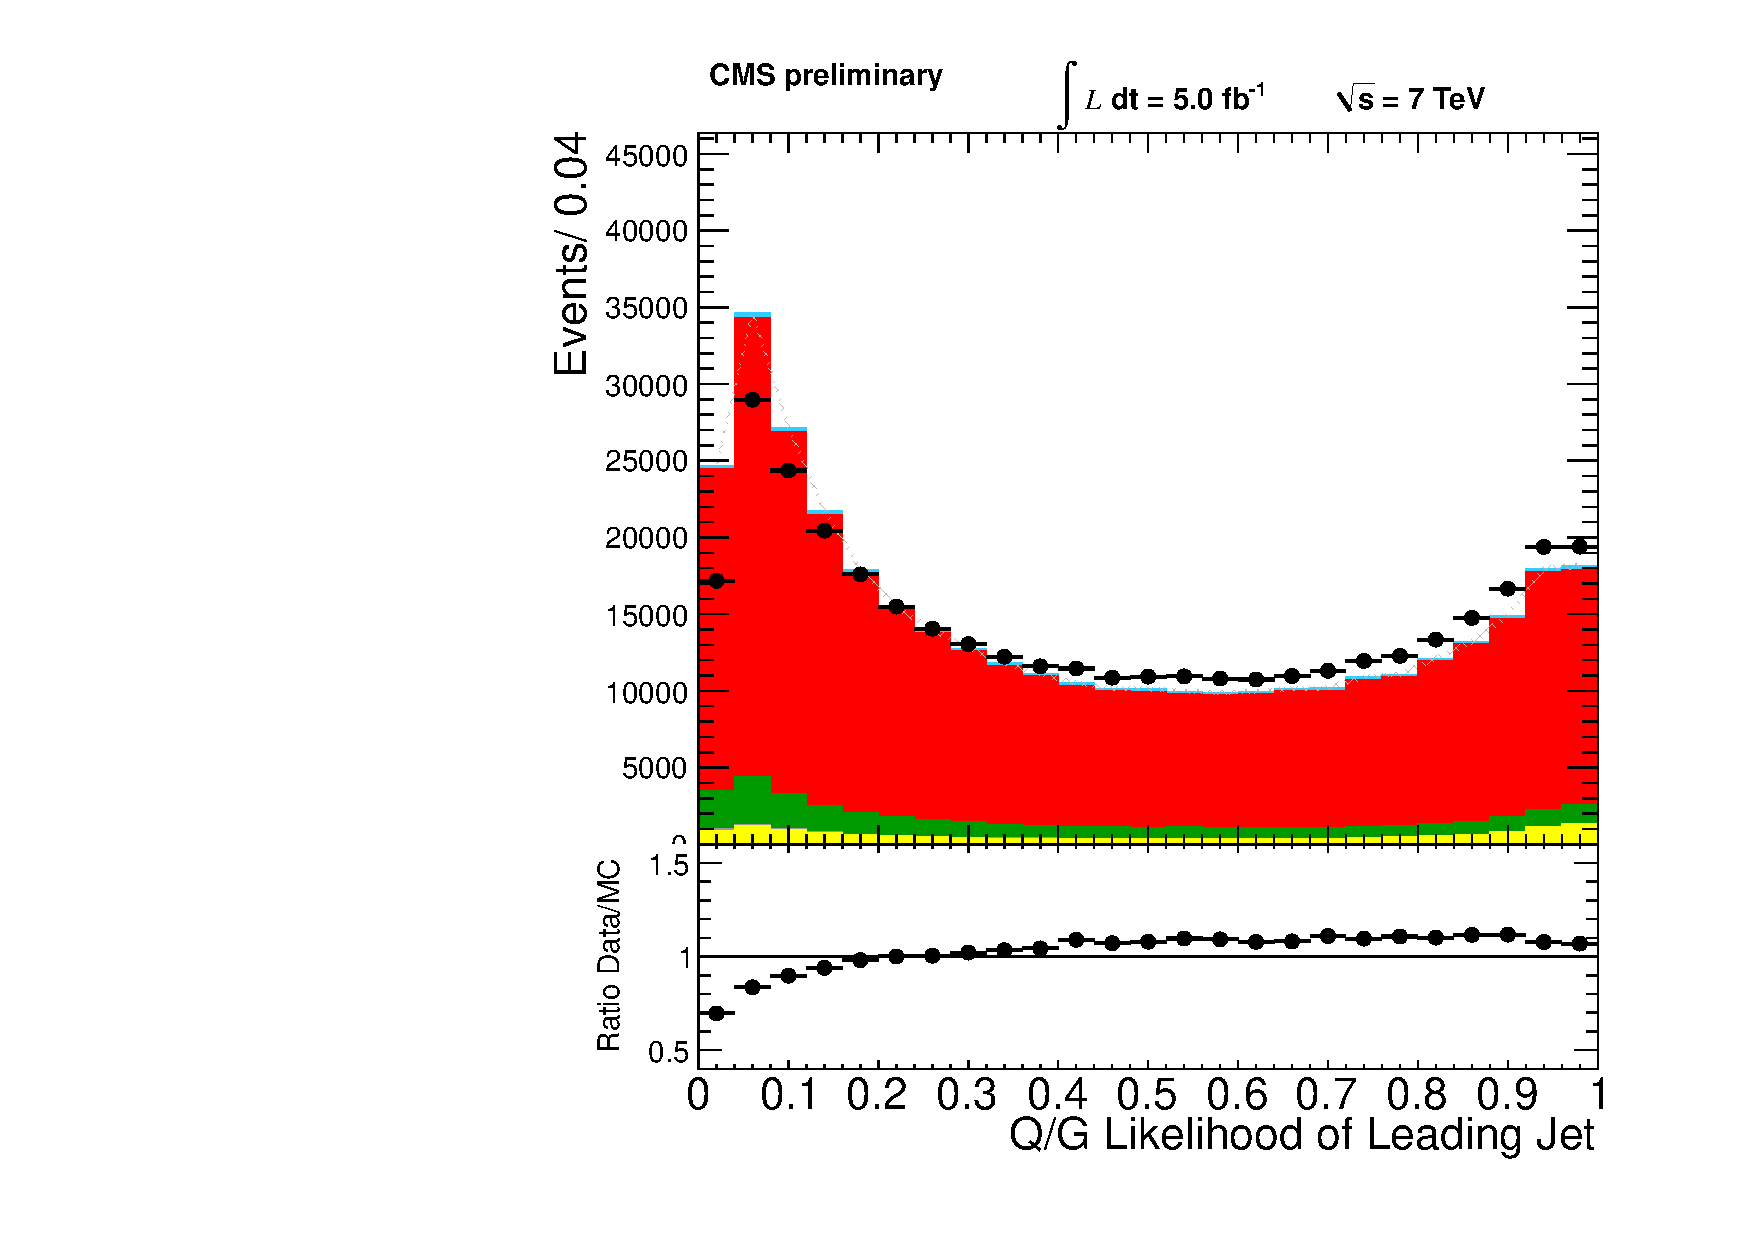
\includegraphics[width=0.49\textwidth]{figs/n-1_plots_mu/mu_jetld_qgl.pdf}
    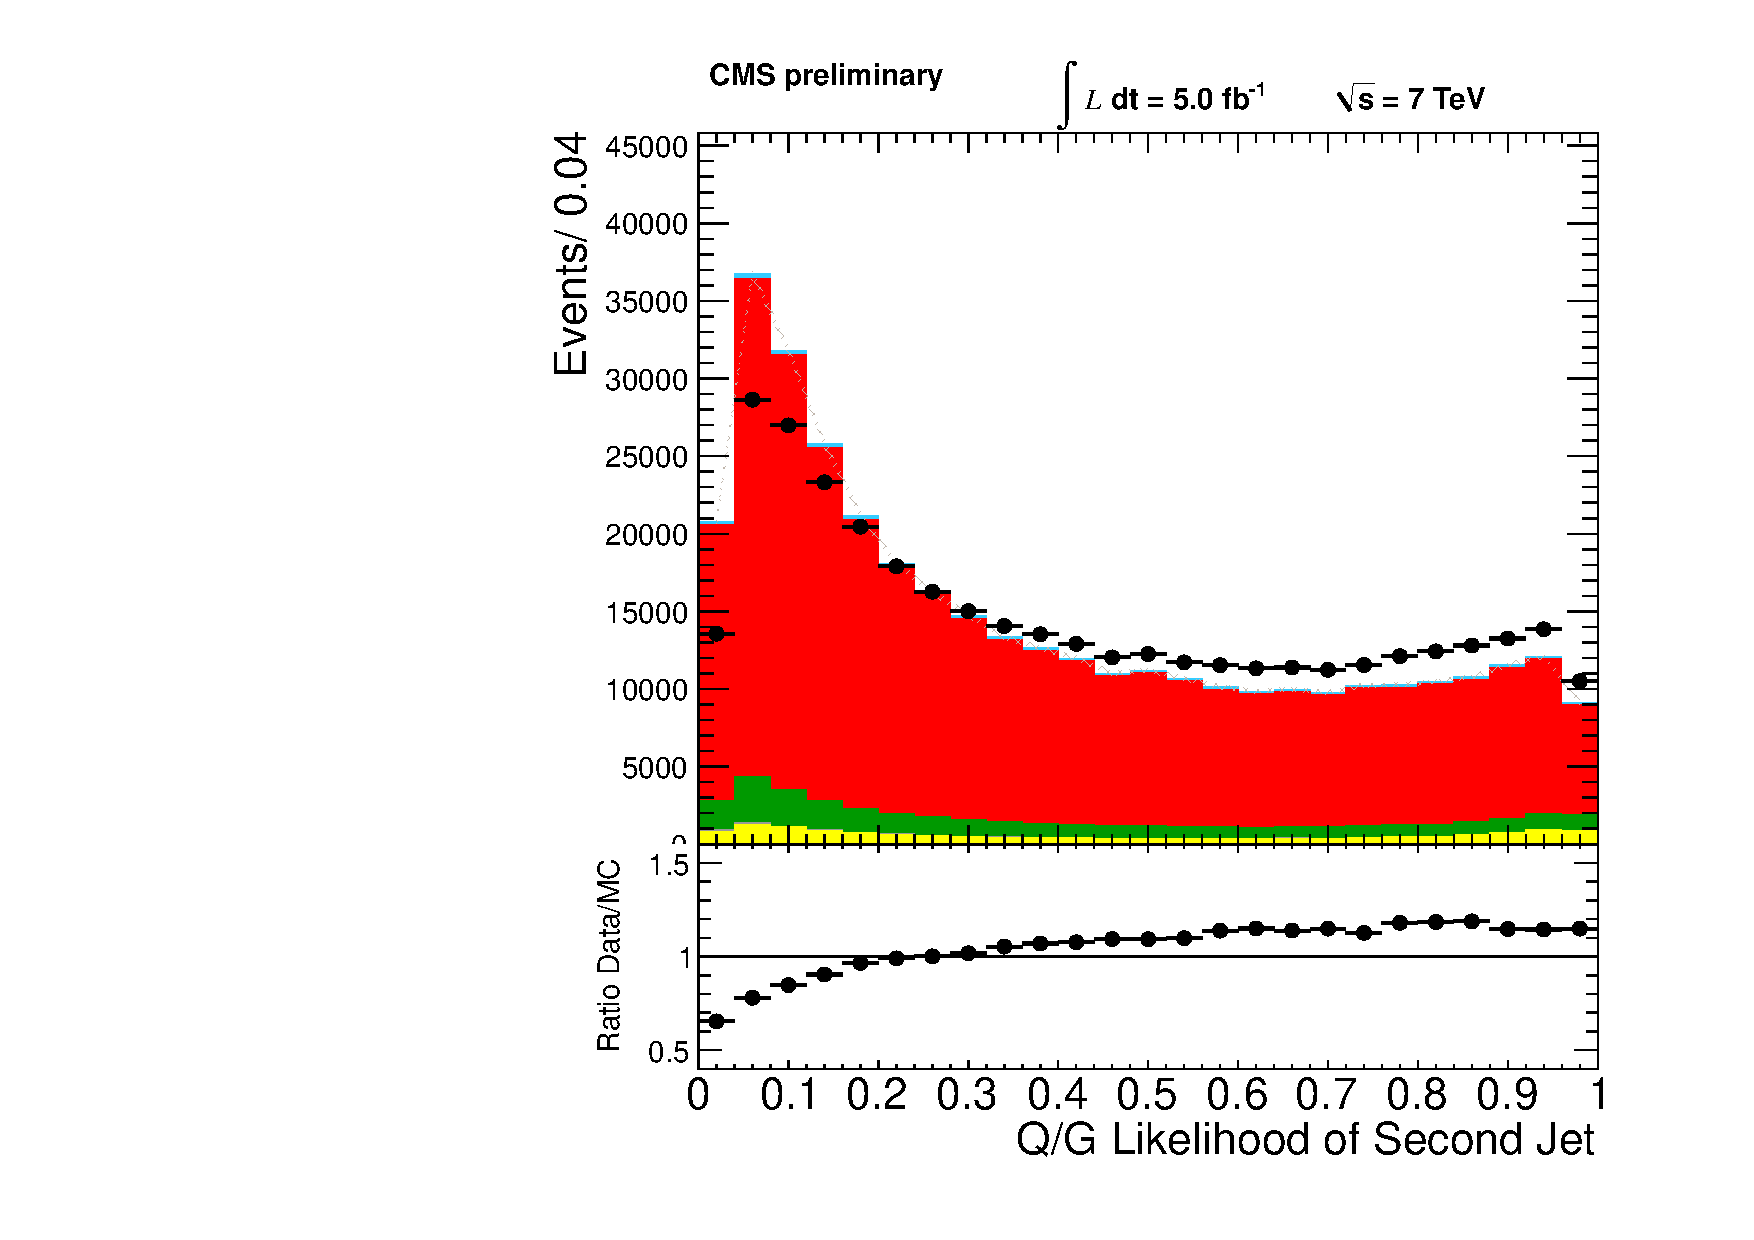
\includegraphics[width=0.49\textwidth]{figs/n-1_plots_mu/mu_jetnt_qgl.pdf}
    \caption{Comparison of the Quark-gluon likelihood distributions for leading jet (left)
    second leading (right) from data and MC for the muon+jets selection.}
\label{fig:mu_jet_qgl}}
\end{figure}
% angular variables
%%%%%%%%%%%%%%%%%%%%%%%%%%%%
\begin{figure}[h!t]
  {\centering
    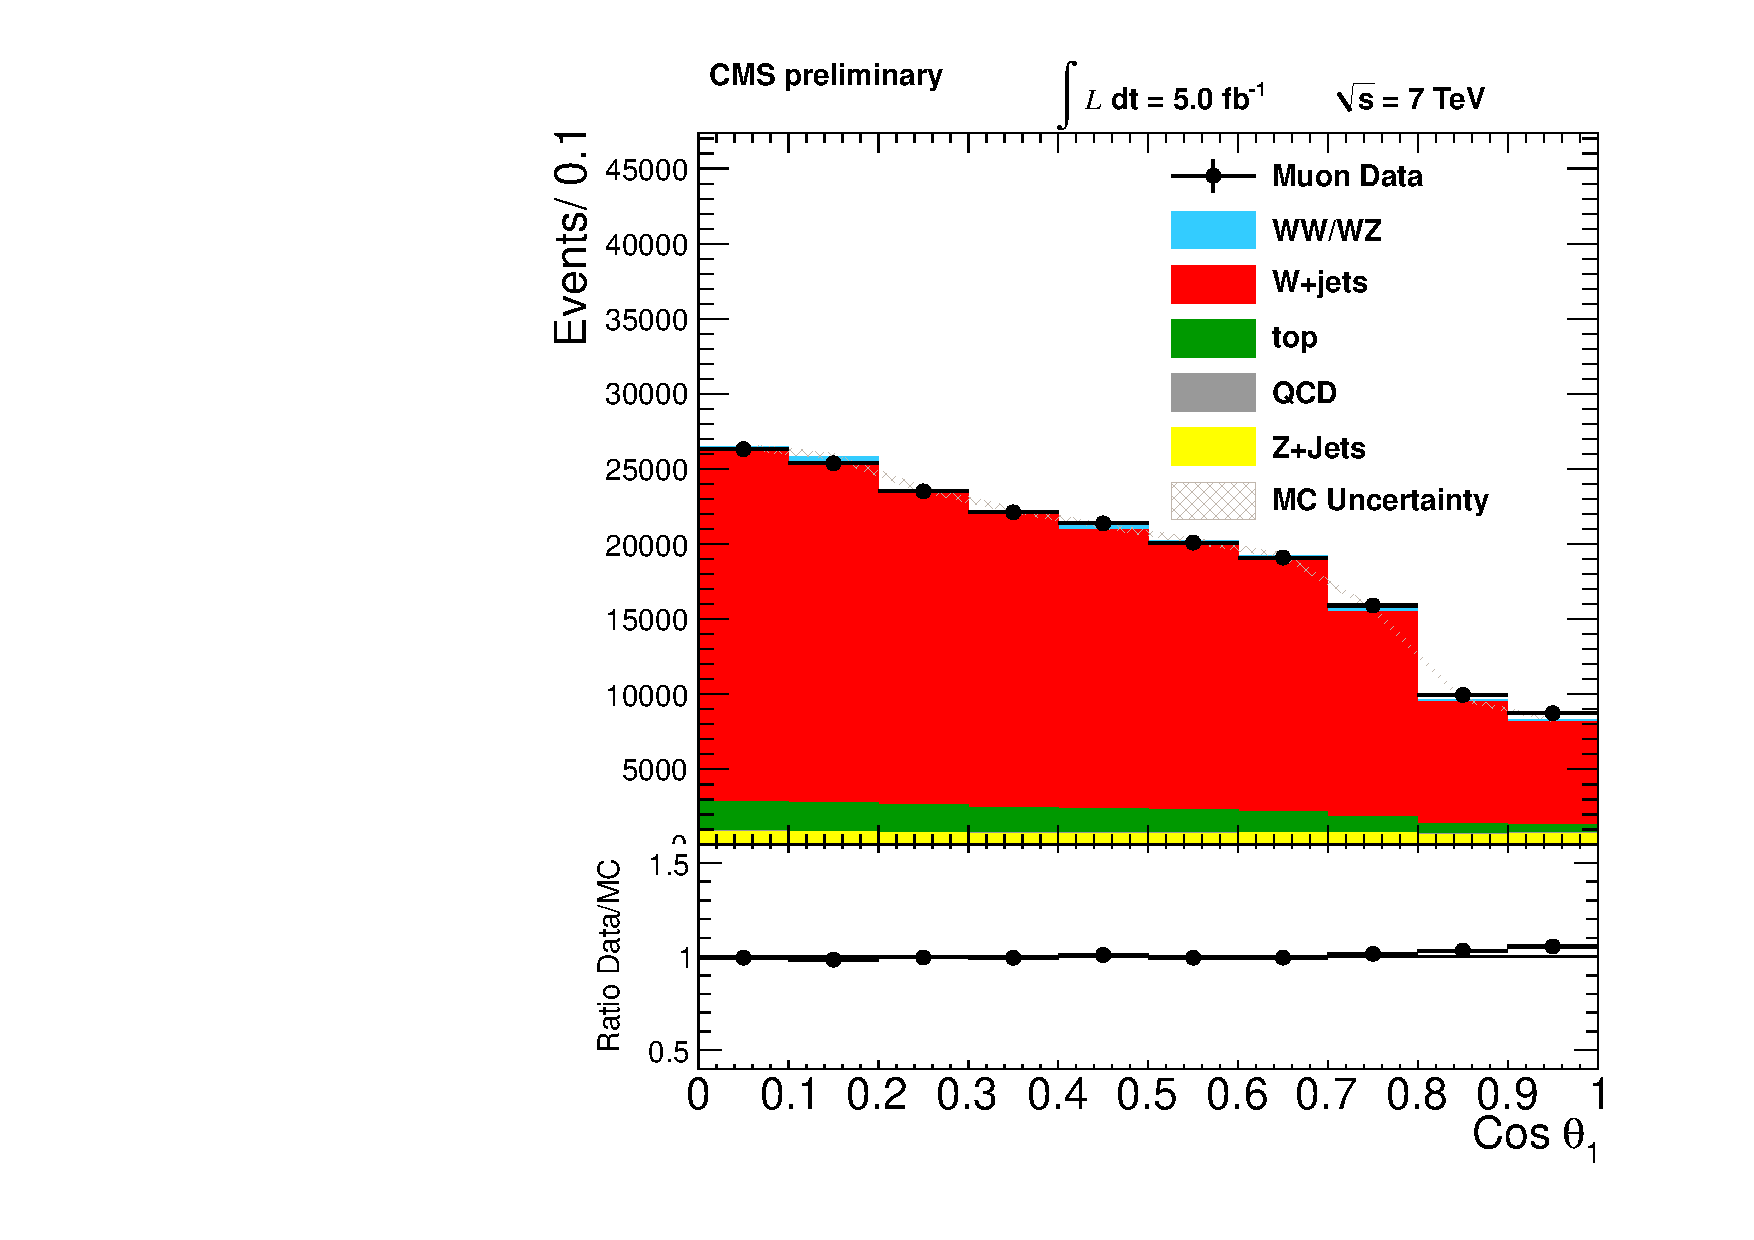
\includegraphics[width=0.49\textwidth]{figs/n-1_plots_mu/mu_ha.pdf}
    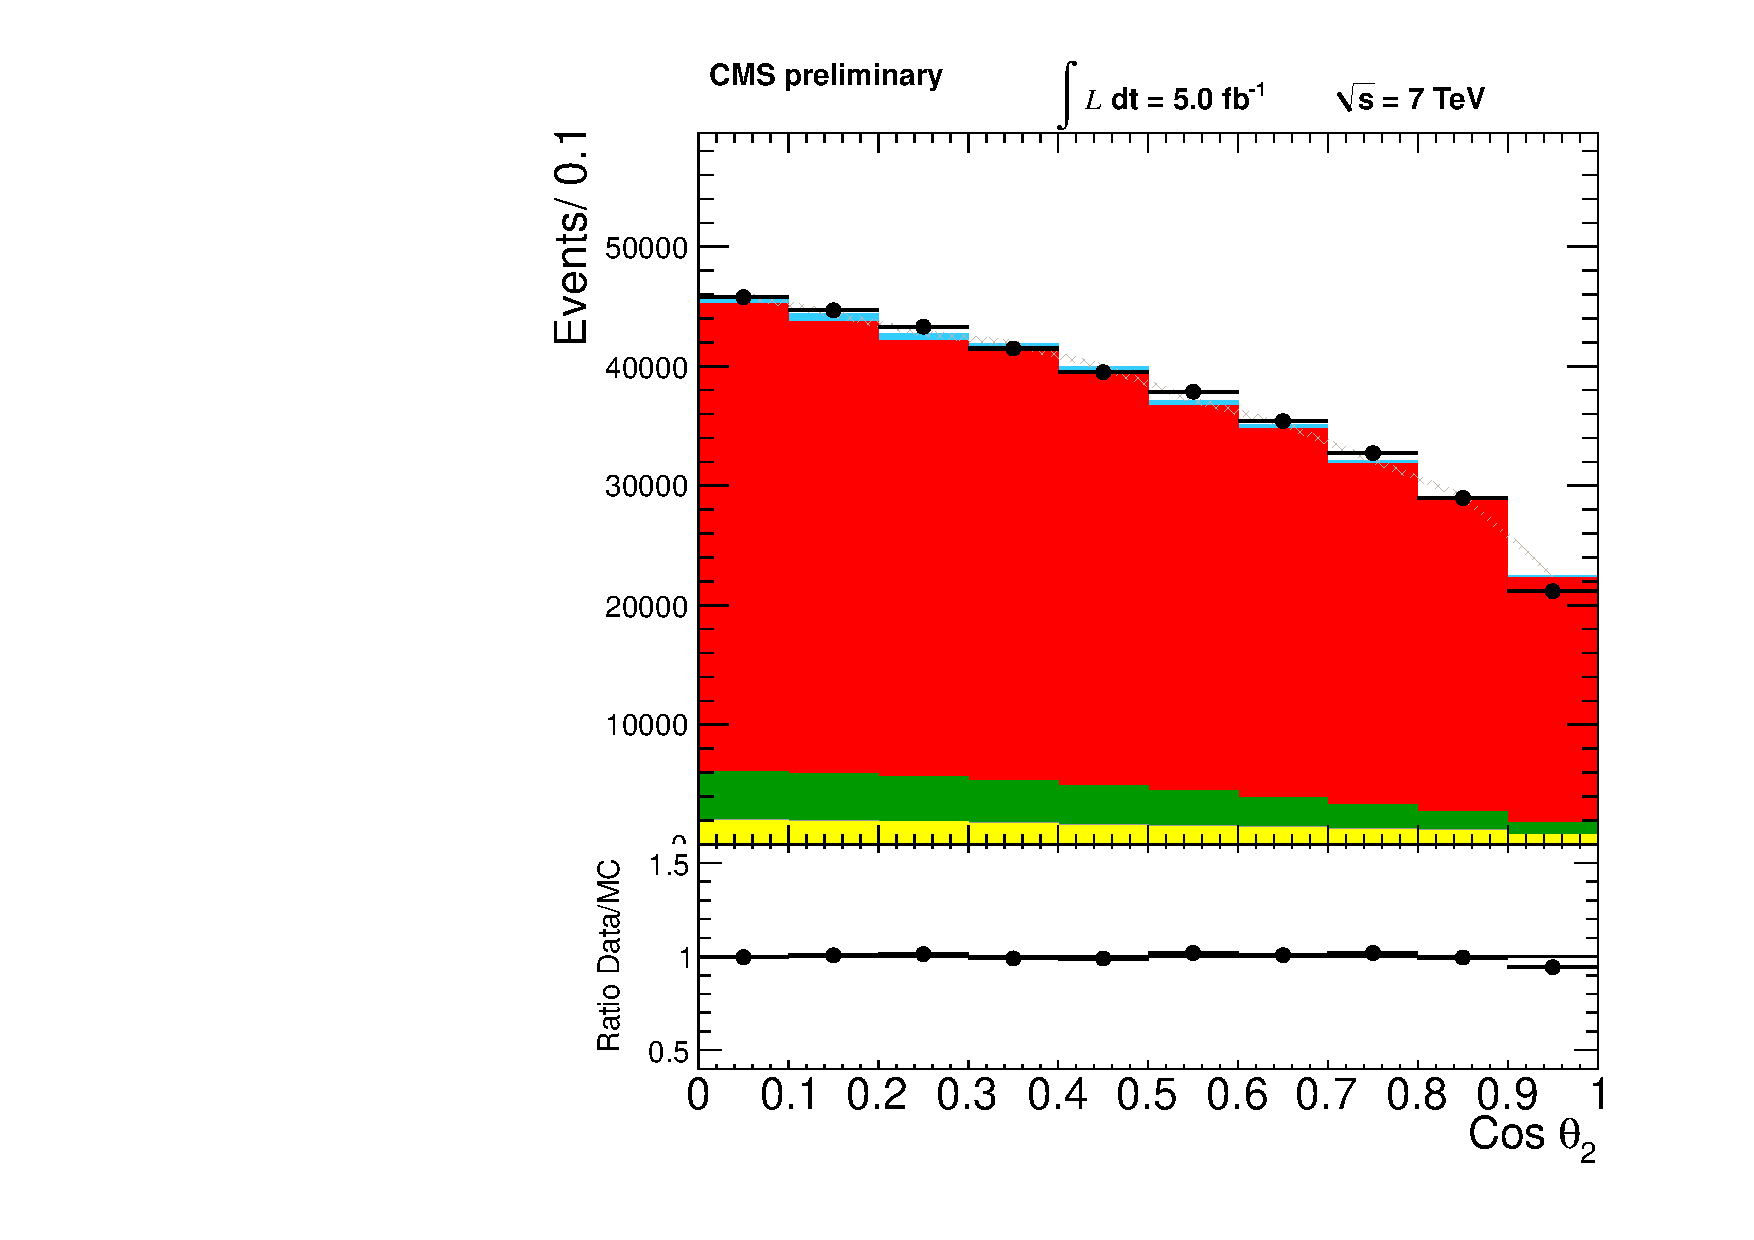
\includegraphics[width=0.49\textwidth]{figs/n-1_plots_mu/mu_hb.pdf}
    \caption{Comparison of the angular distributions for $\cos\theta_{1}$ (left)
   $\cos\theta_{2}$ (right) from data and MC for the muon+jets selection.}
\label{fig:mu_theta}}
\end{figure}
%%%%%%%%%%%%%%%%%%%%%%%%%%%%
\begin{figure}[h!t]
  {\centering
     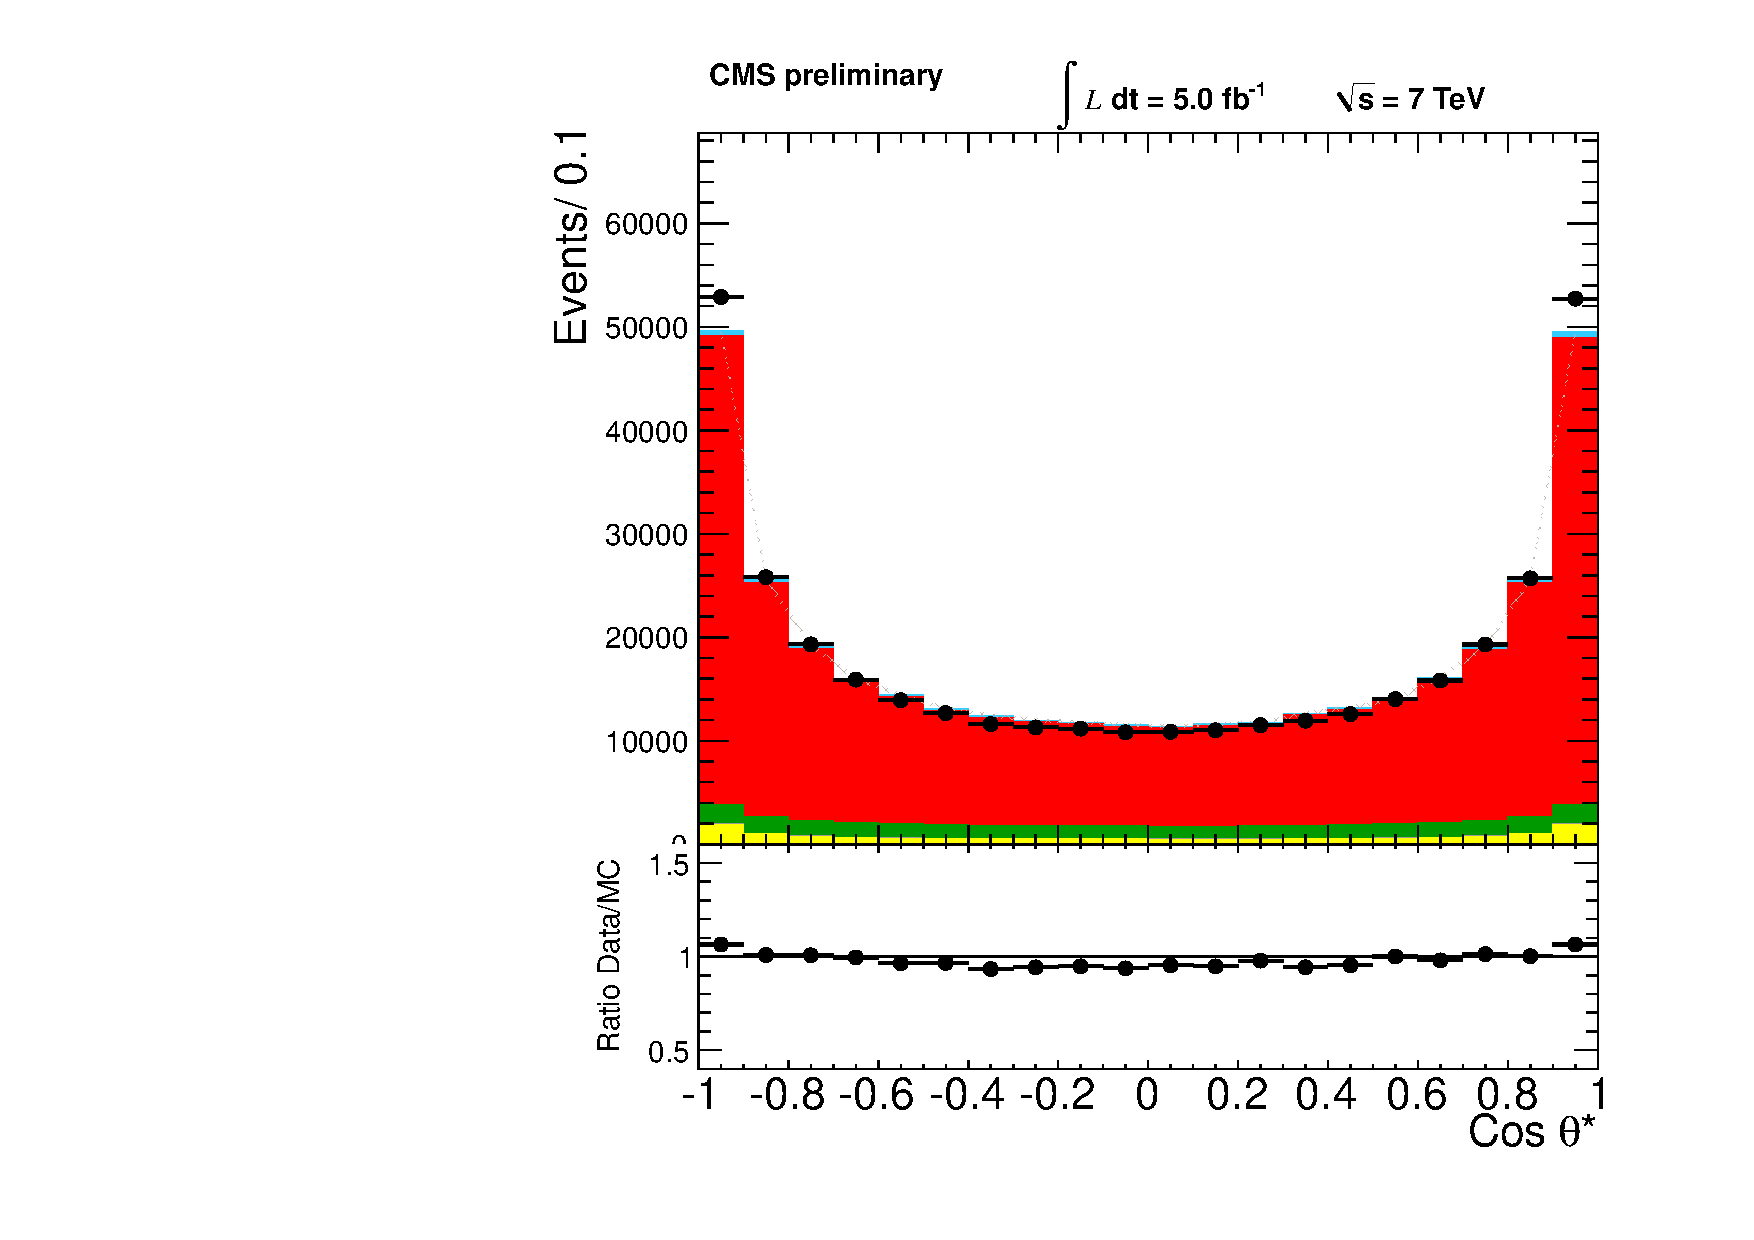
\includegraphics[width=0.49\textwidth]{figs/n-1_plots_mu/mu_hs.pdf}
    \caption{Comparison of the angular distributions for $\cos\theta^{\ast}$ from data and MC 
   for the muon+jets selection.}
\label{fig:mu_thetas}}
\end{figure}
%%%%%%%%%%%%%%%%%%%%%%%%%%%%
\begin{figure}[h!t]
  {\centering
    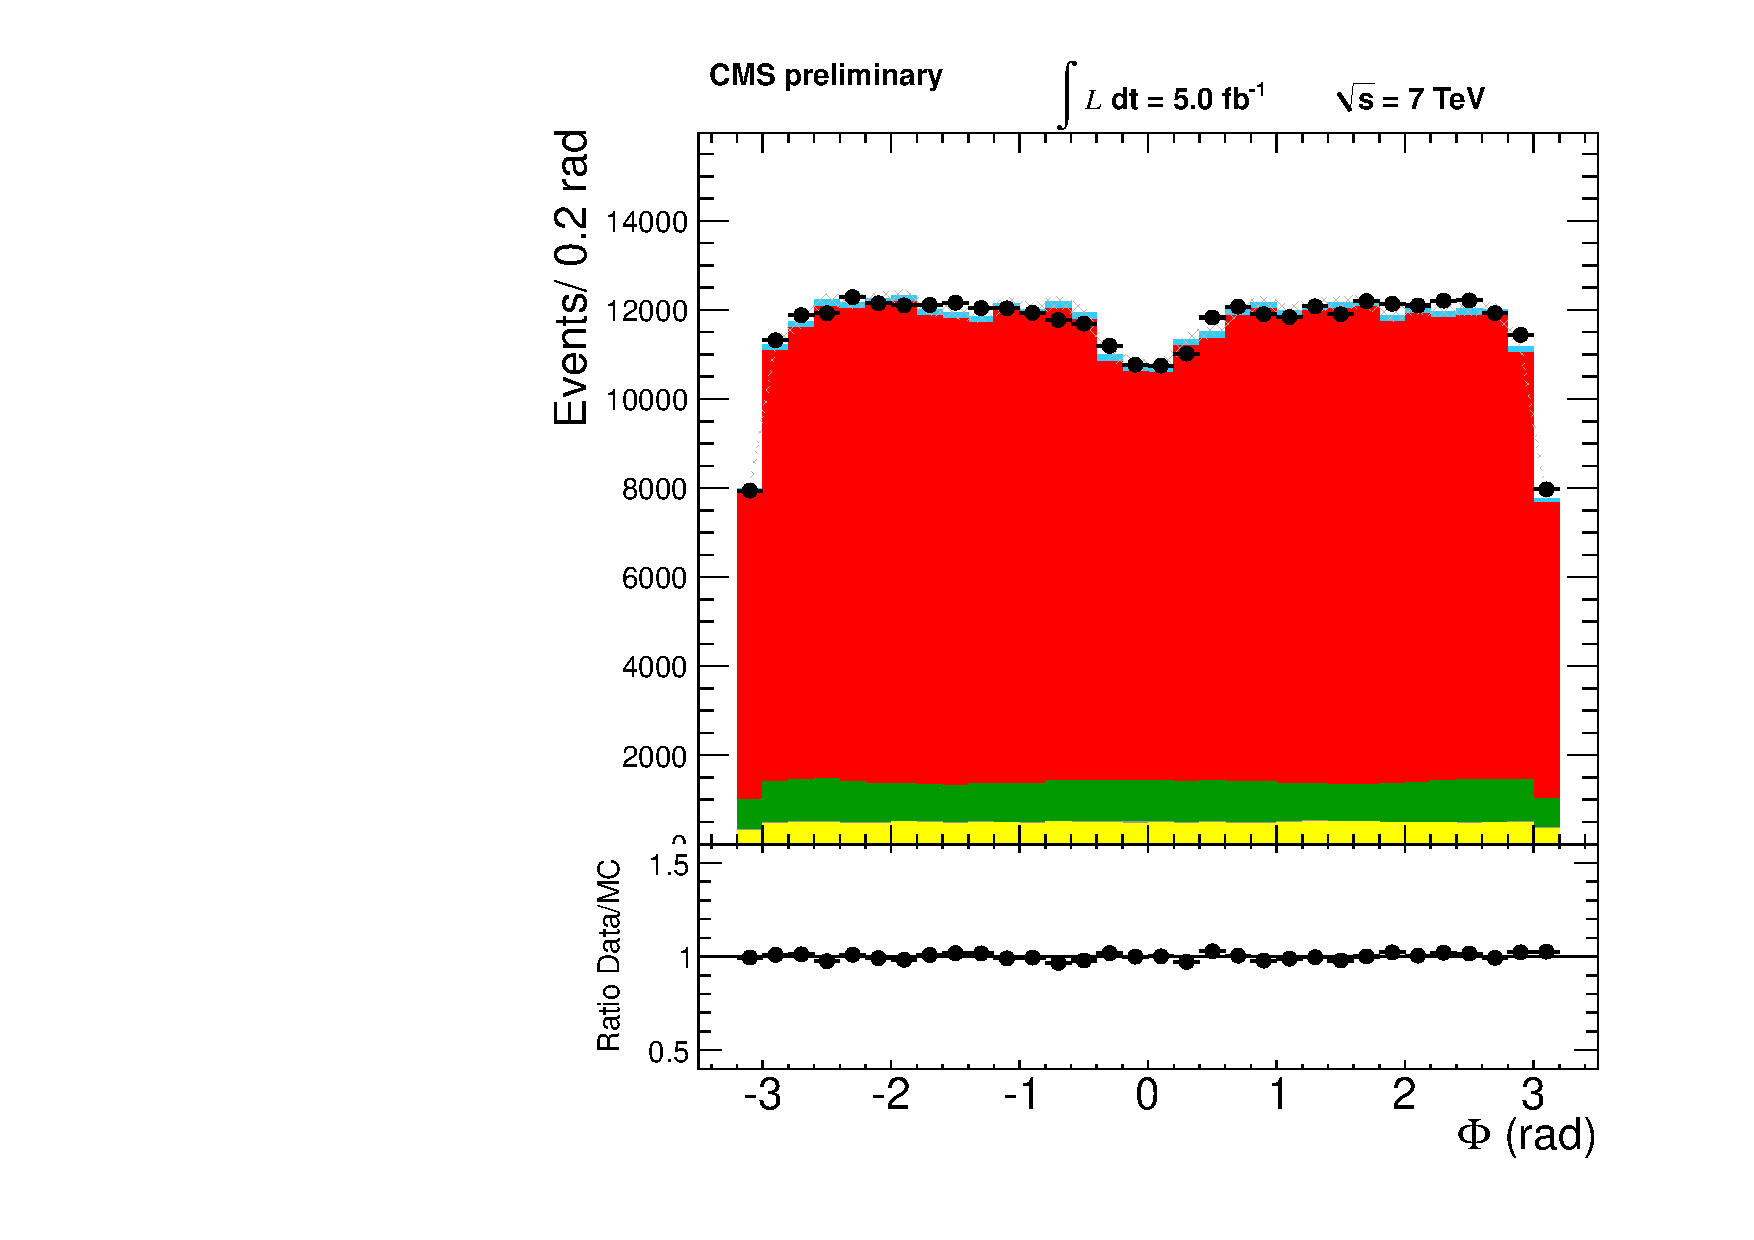
\includegraphics[width=0.49\textwidth]{figs/n-1_plots_mu/mu_phi.pdf}
    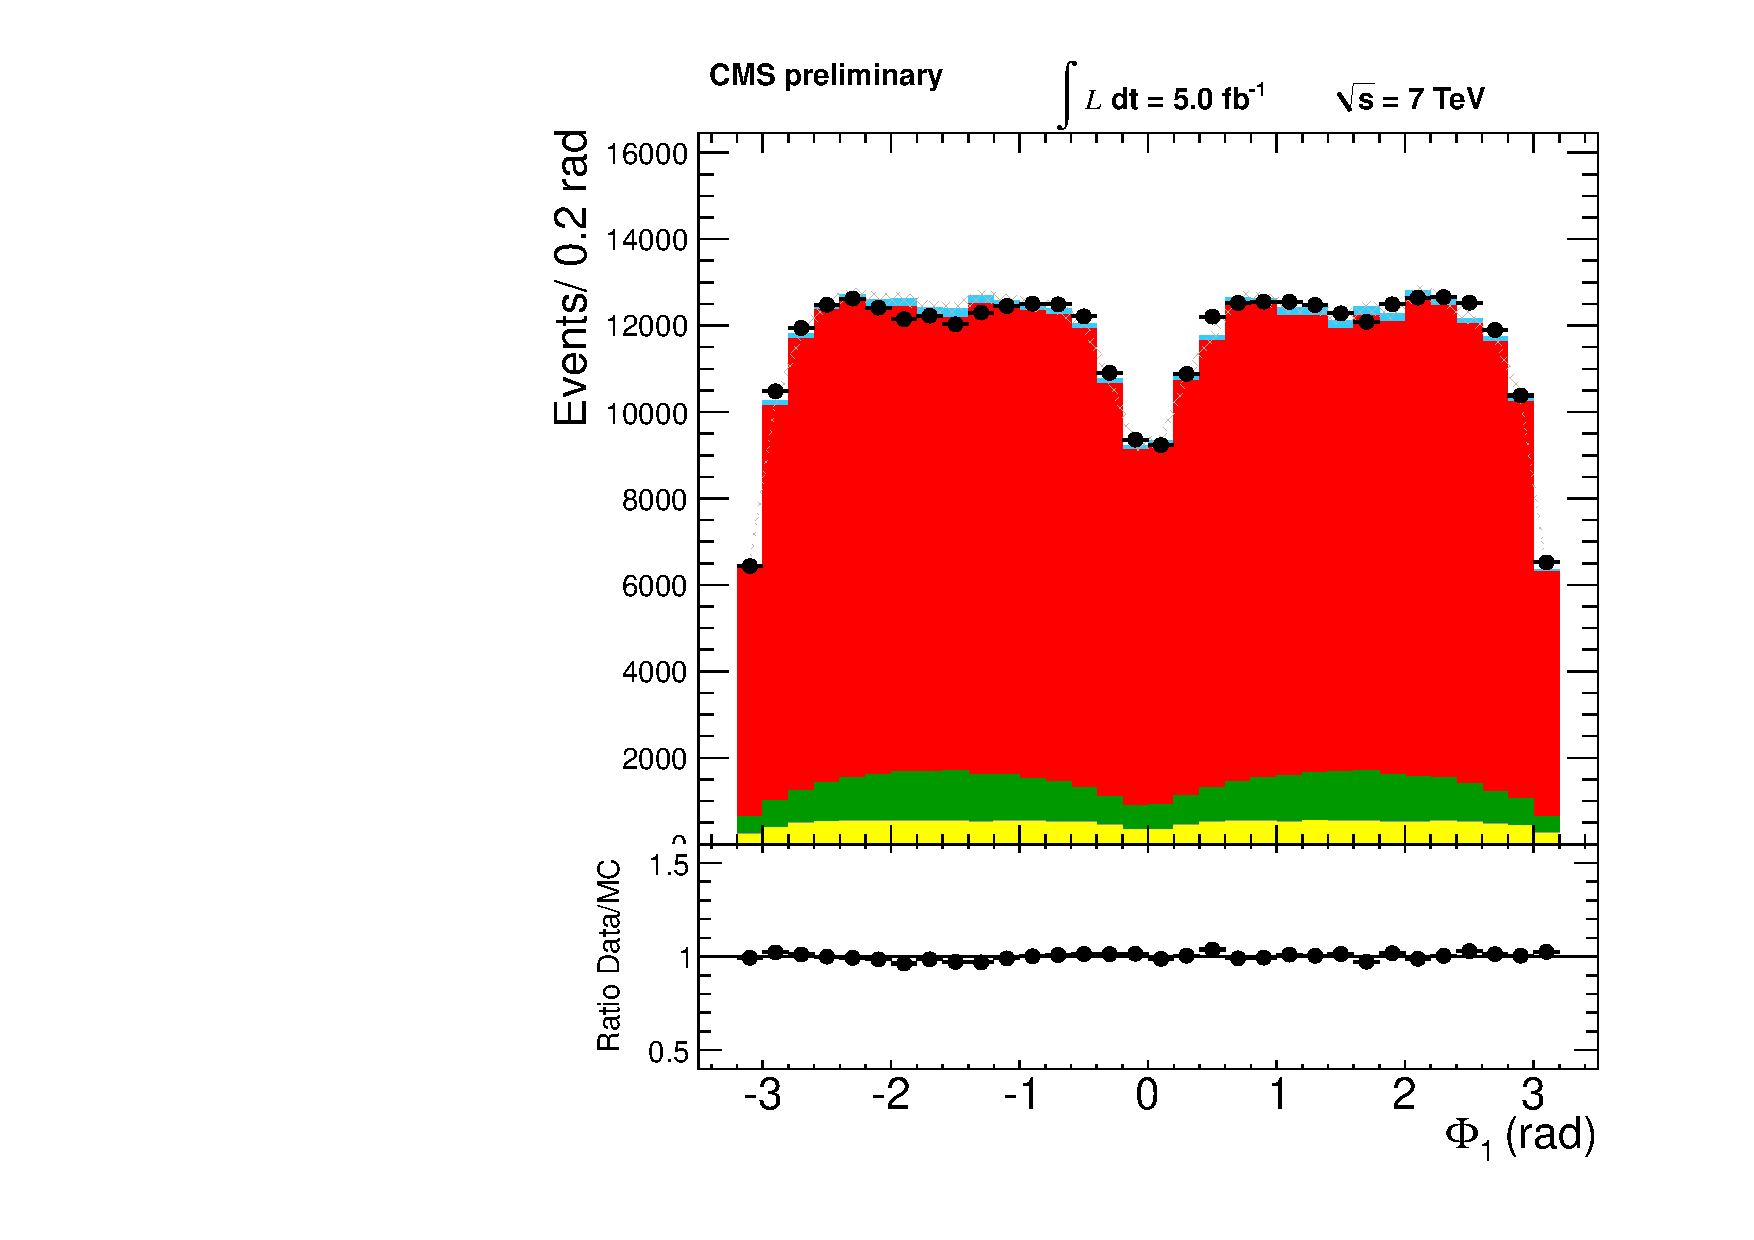
\includegraphics[width=0.49\textwidth]{figs/n-1_plots_mu/mu_phib.pdf}
    \caption{Comparison of the angular distributions for $\Phi$  (left)$\Phi_{1}$ (right) from data and 
      MC for the muon+jets selection.}
\label{fig:mu_phi}}
\end{figure}

%%%%%%%%%%%%%%%%%%%%%%%%%%%%
\begin{figure}[h!t]
  {\centering
    \includegraphics[width=0.49\textwidth]{figs/n-1_plots_mu/mu_charge.pdf}
    \caption{Comparison of the charge of the muon from data and MC for the muon+jets selection.}
\label{fig:mu_chg}}
\end{figure}

% rapidity and pt of the WW system

%%%%%%%%%%%%%%%%%%%%%%%%%%%%
\begin{figure}[h!t]
  {\centering
    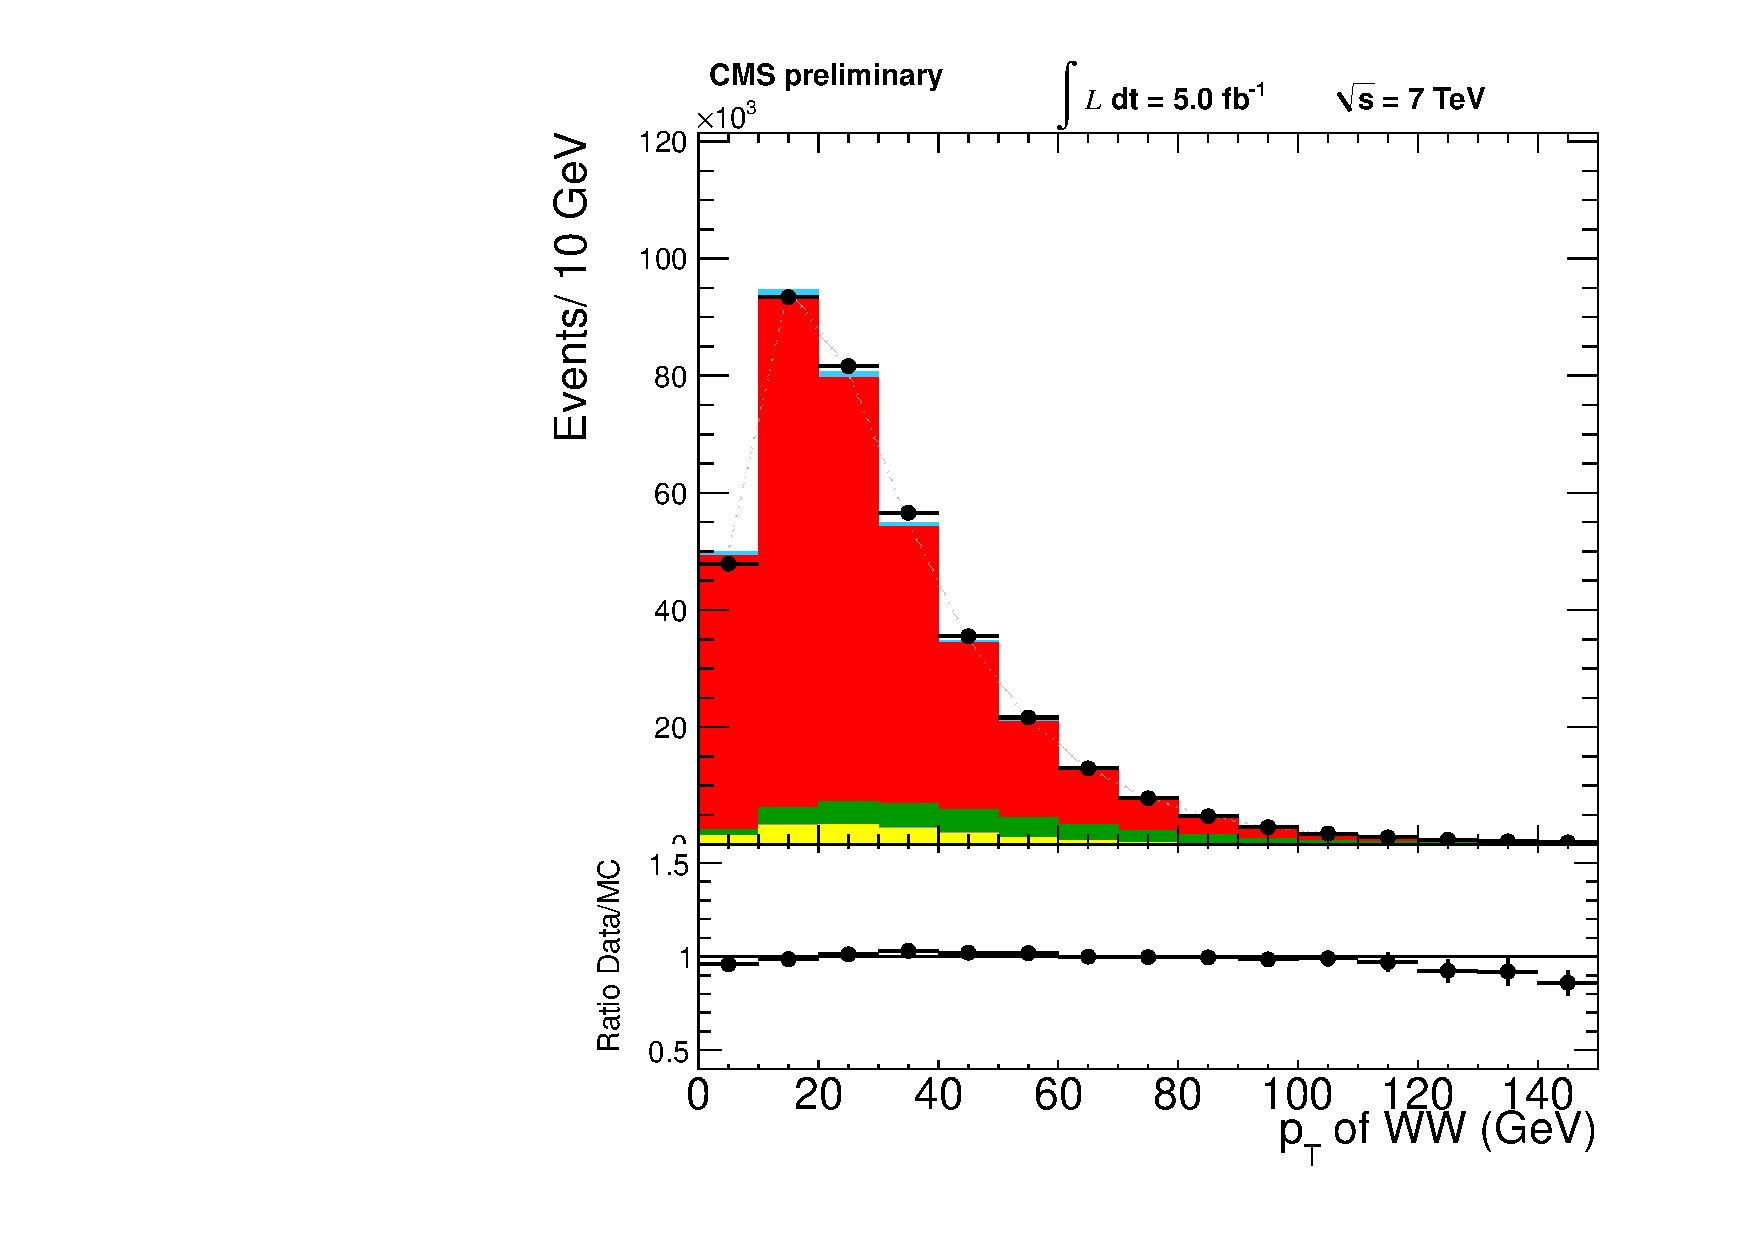
\includegraphics[width=0.49\textwidth]{figs/n-1_plots_mu/mu_ptlvjj.pdf}
    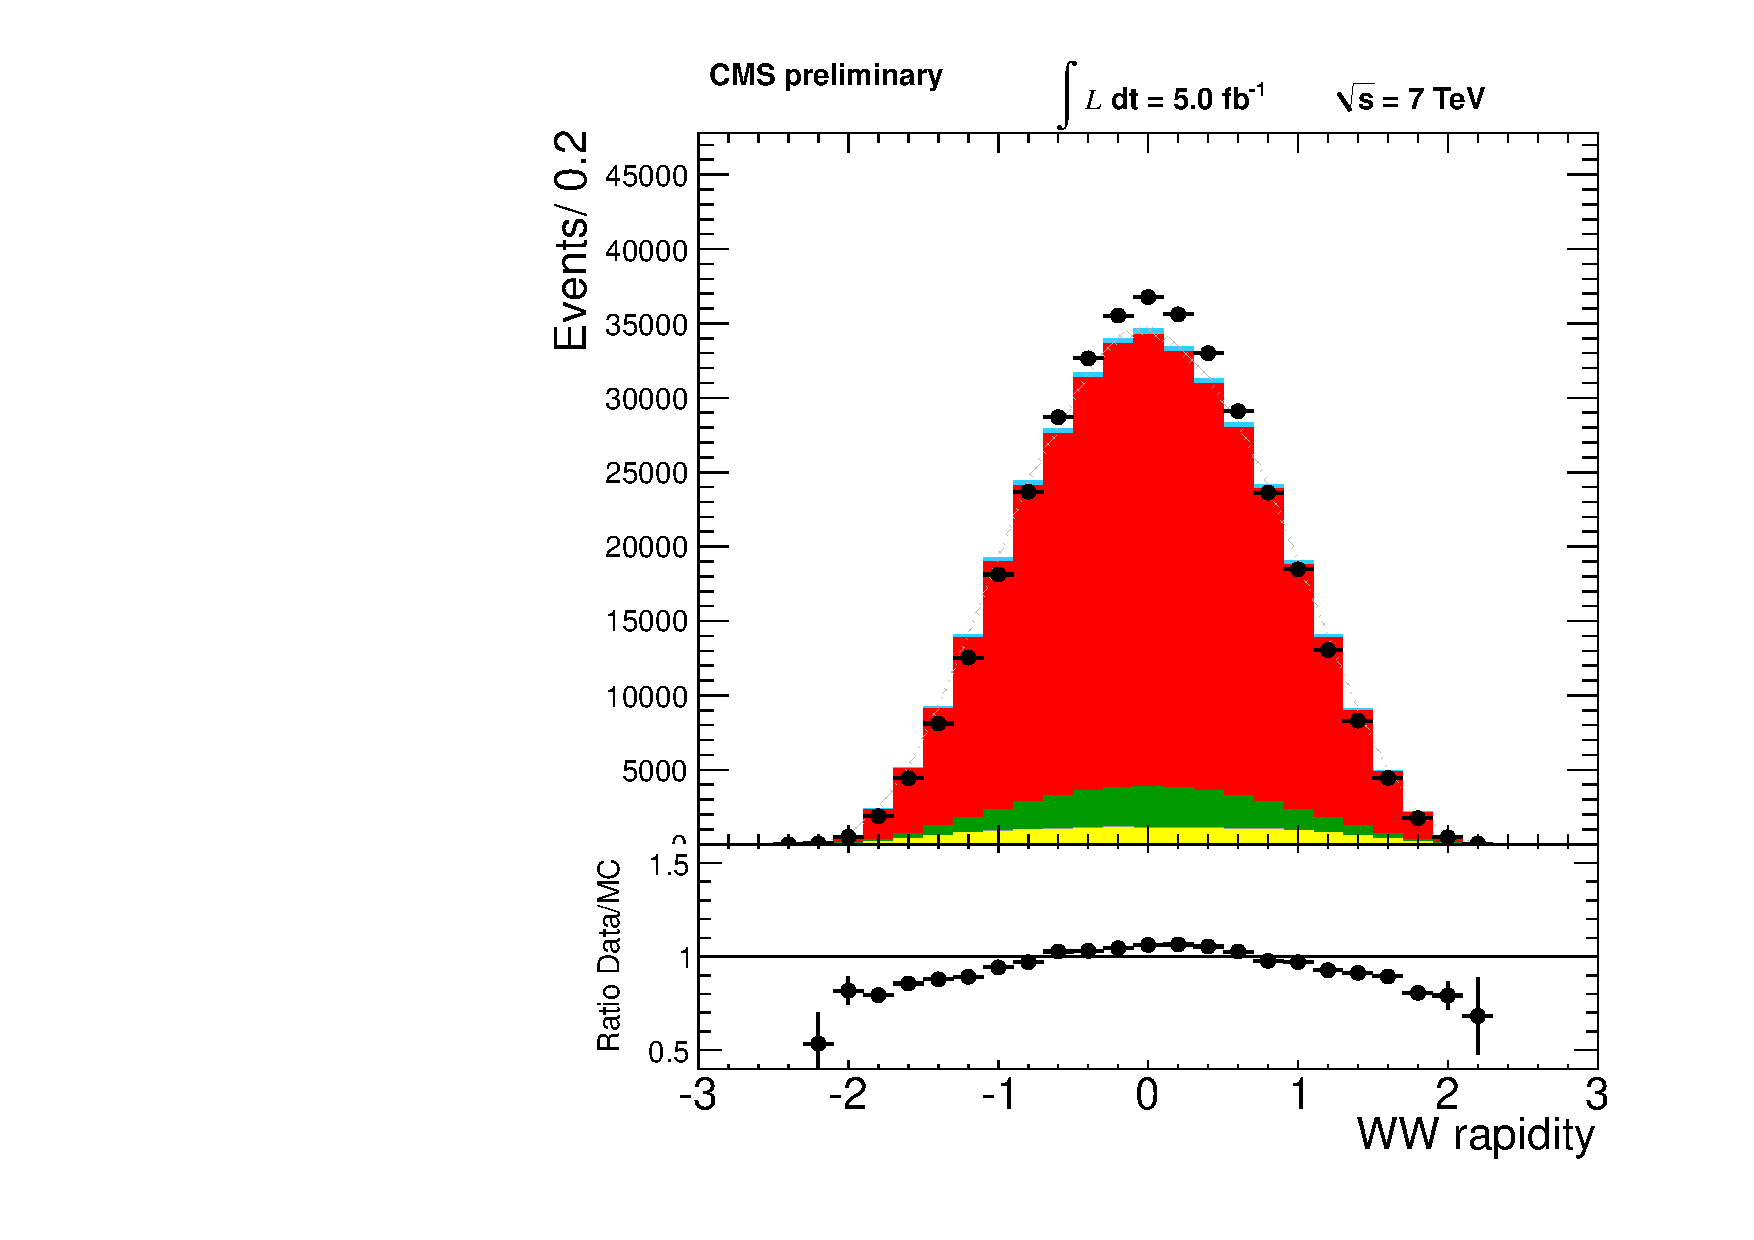
\includegraphics[width=0.49\textwidth]{figs/n-1_plots_mu/mu_etalvjj.pdf}
    \caption{Comparison of the $p_{T}$ (left) $\eta$ (right) of the WW system
      from data and MC for the muon+jets selection.}
\label{fig:mu_ww}}
\end{figure}

%%%%%%%%%%%%%%%%%%%%%%%%%%%%%%%%%
%%%%%%%%%%%%%%%%%%%%%%%

% quark-gluon discriminants
%%%%%%%%%%%%%%%%%%%%%%%%%%%%
\begin{figure}[h!t]
  {\centering
    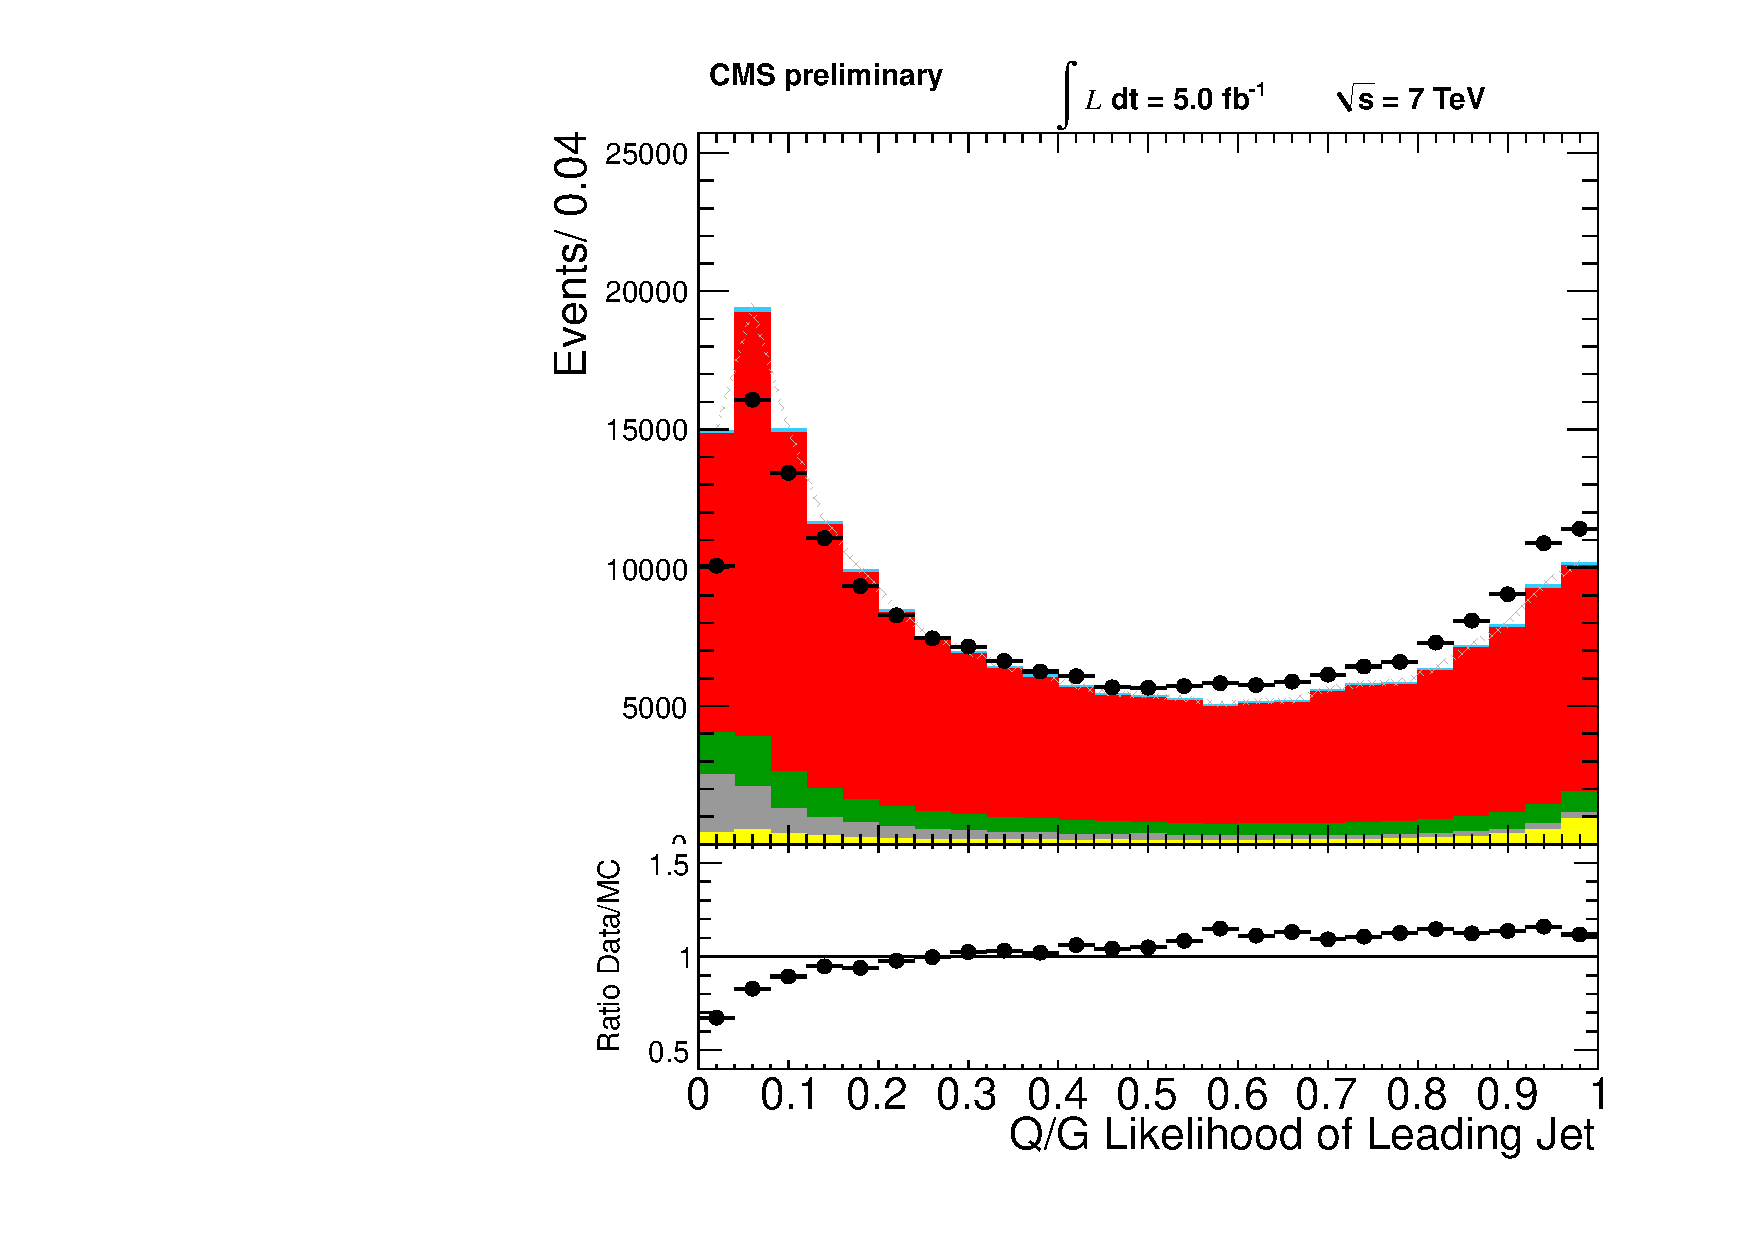
\includegraphics[width=0.49\textwidth]{figs/n-1_plots_el/el_jetld_qgl.pdf}
    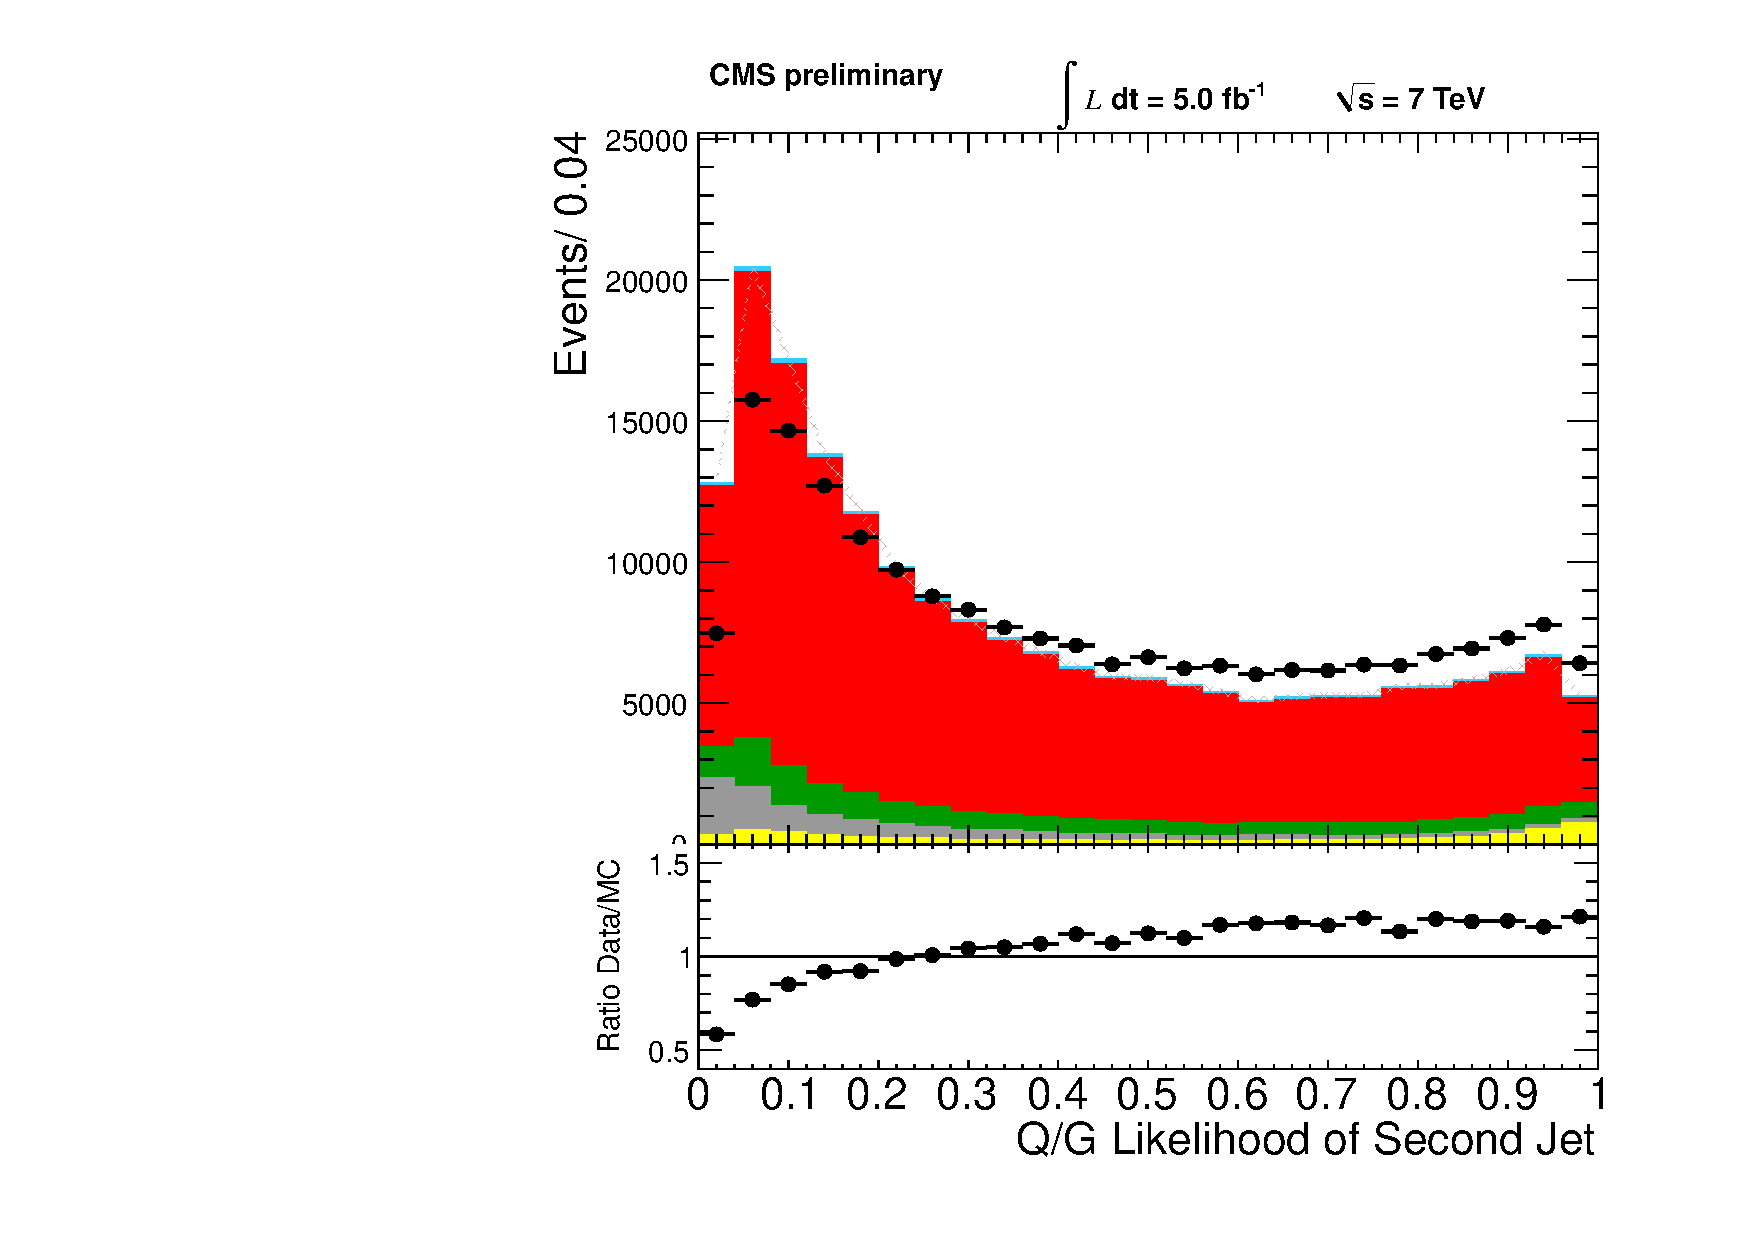
\includegraphics[width=0.49\textwidth]{figs/n-1_plots_el/el_jetnt_qgl.pdf}
    \caption{Comparison of the Quark-gluon likelihood distributions for leading jet (left)
    second leading (right) from data and MC for the electron+jets selection.}
\label{fig:elec_jet_qgl}}
\end{figure}
% angular variables
%%%%%%%%%%%%%%%%%%%%%%%%%%%%
%%%%%%%%%%%%%%%%%%%%%%%%%%%%
\begin{figure}[h!t]
  {\centering
    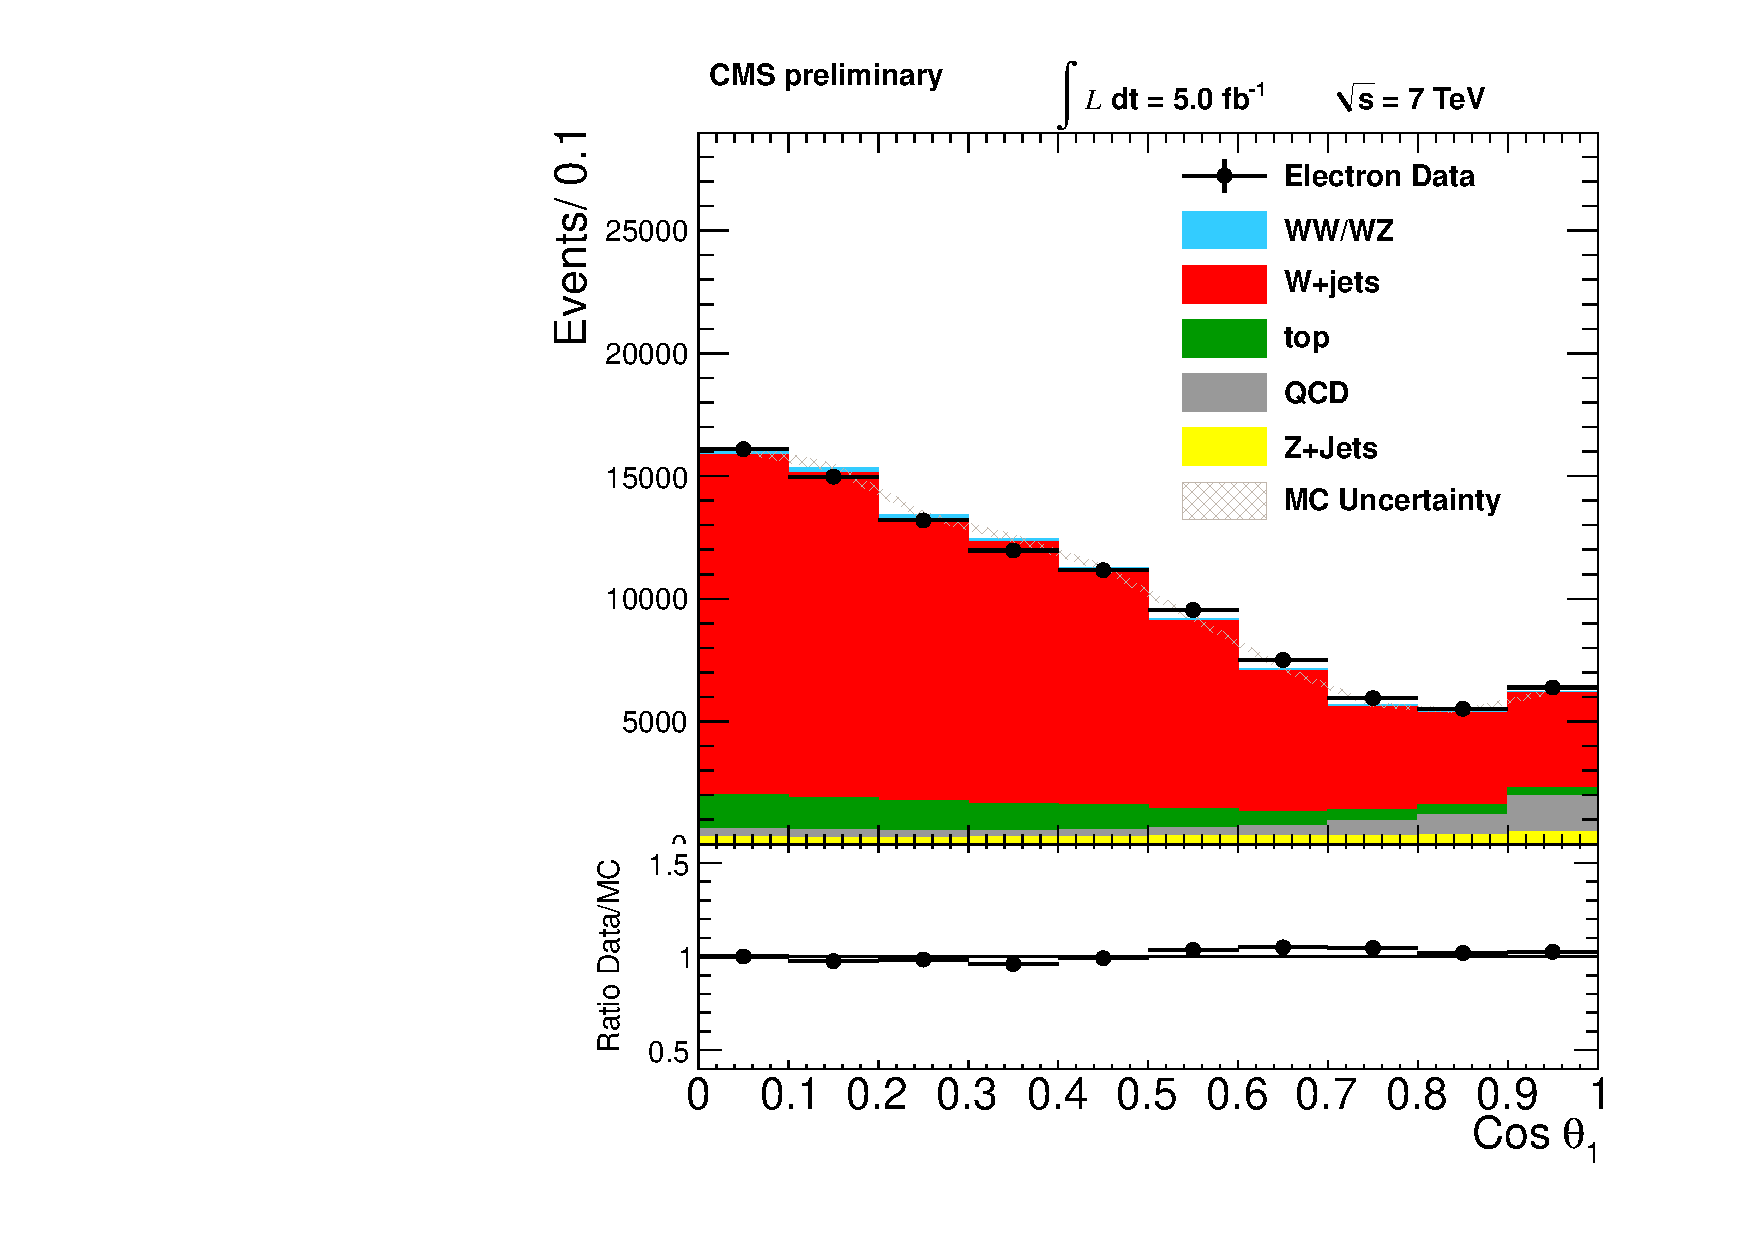
\includegraphics[width=0.49\textwidth]{figs/n-1_plots_el/el_ha.pdf}
    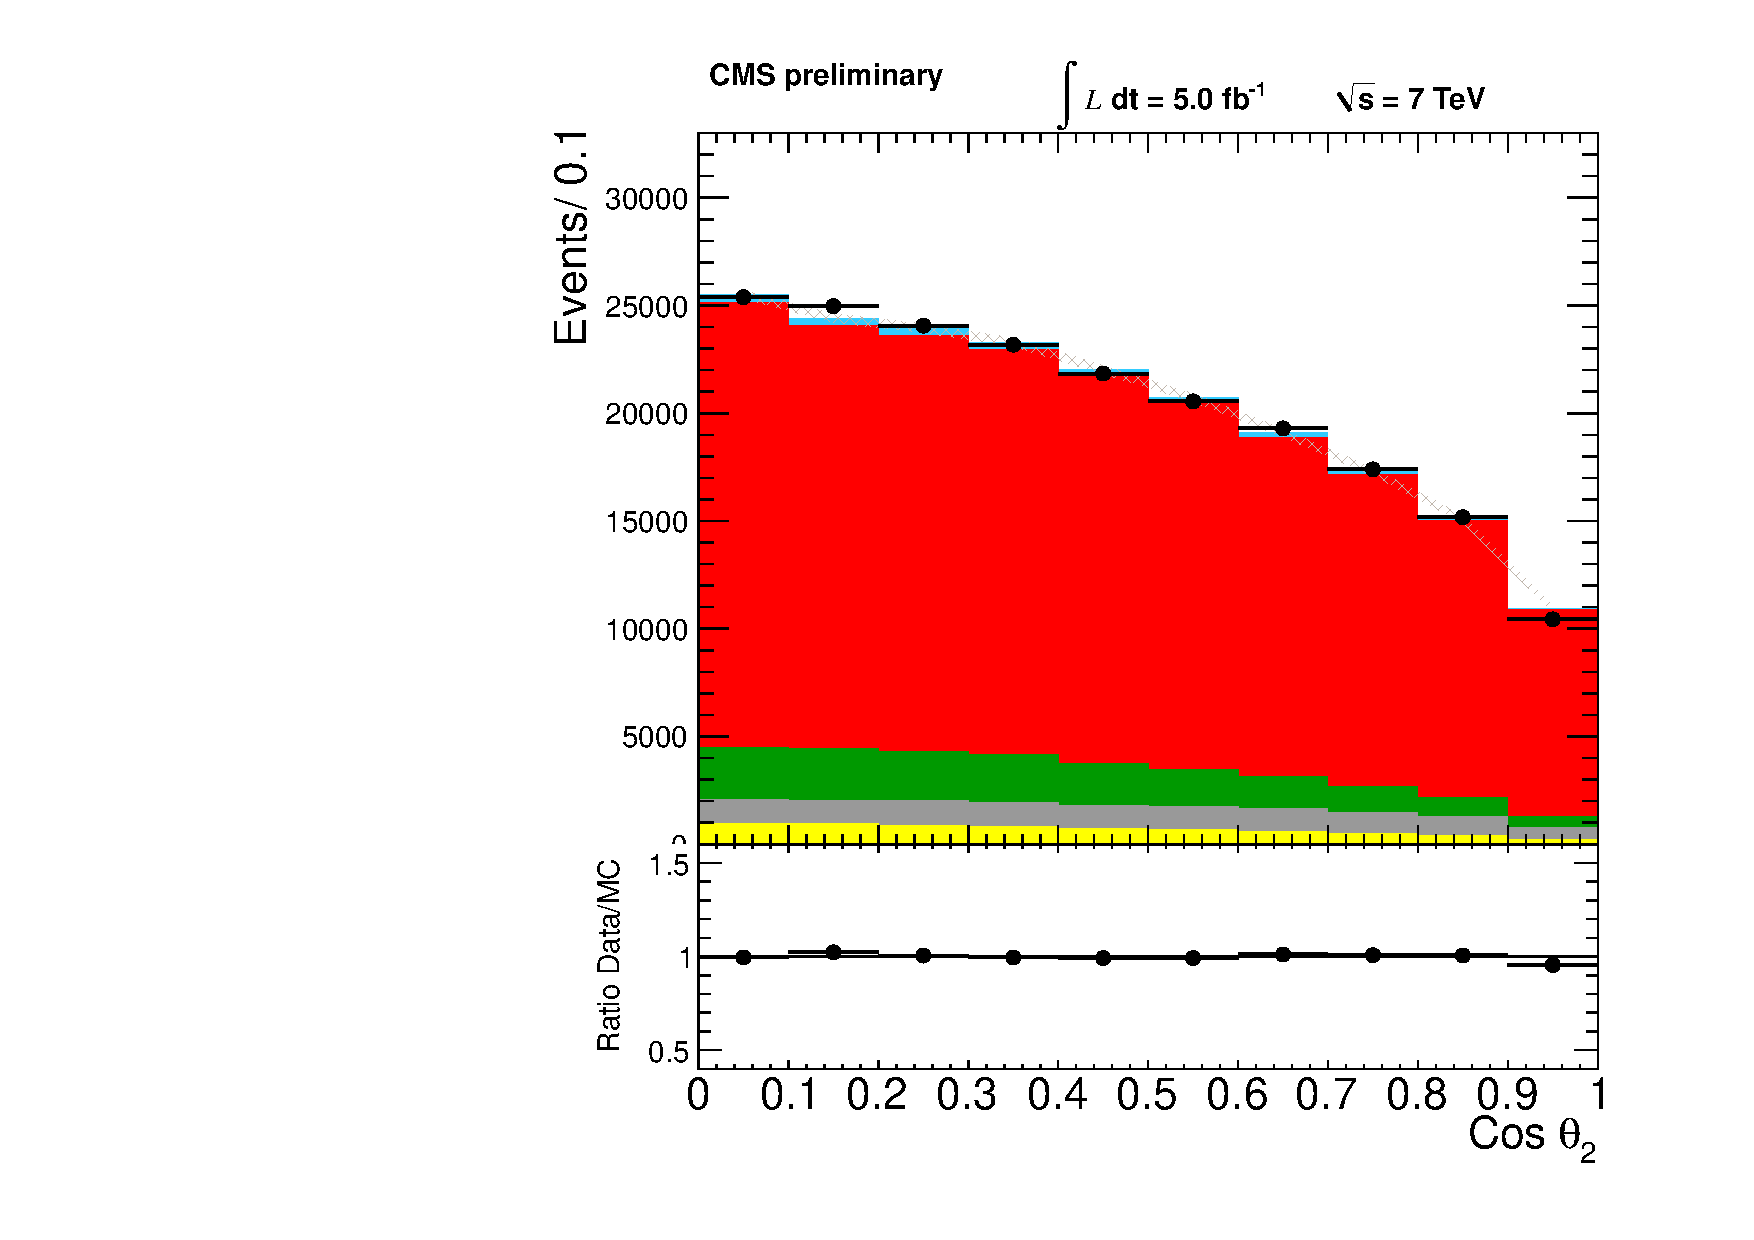
\includegraphics[width=0.49\textwidth]{figs/n-1_plots_el/el_hb.pdf}
    \caption{Comparison of the angular distributions for $\cos\theta_{1}$ (left)
   $\cos\theta_{2}$ (right) from data and MC for the electron+jets selection.}
\label{fig:elec_theta}}
\end{figure}
%%%%%%%%%%%%%%%%%%%%%%%%%%%%
\begin{figure}[h!t]
  {\centering
     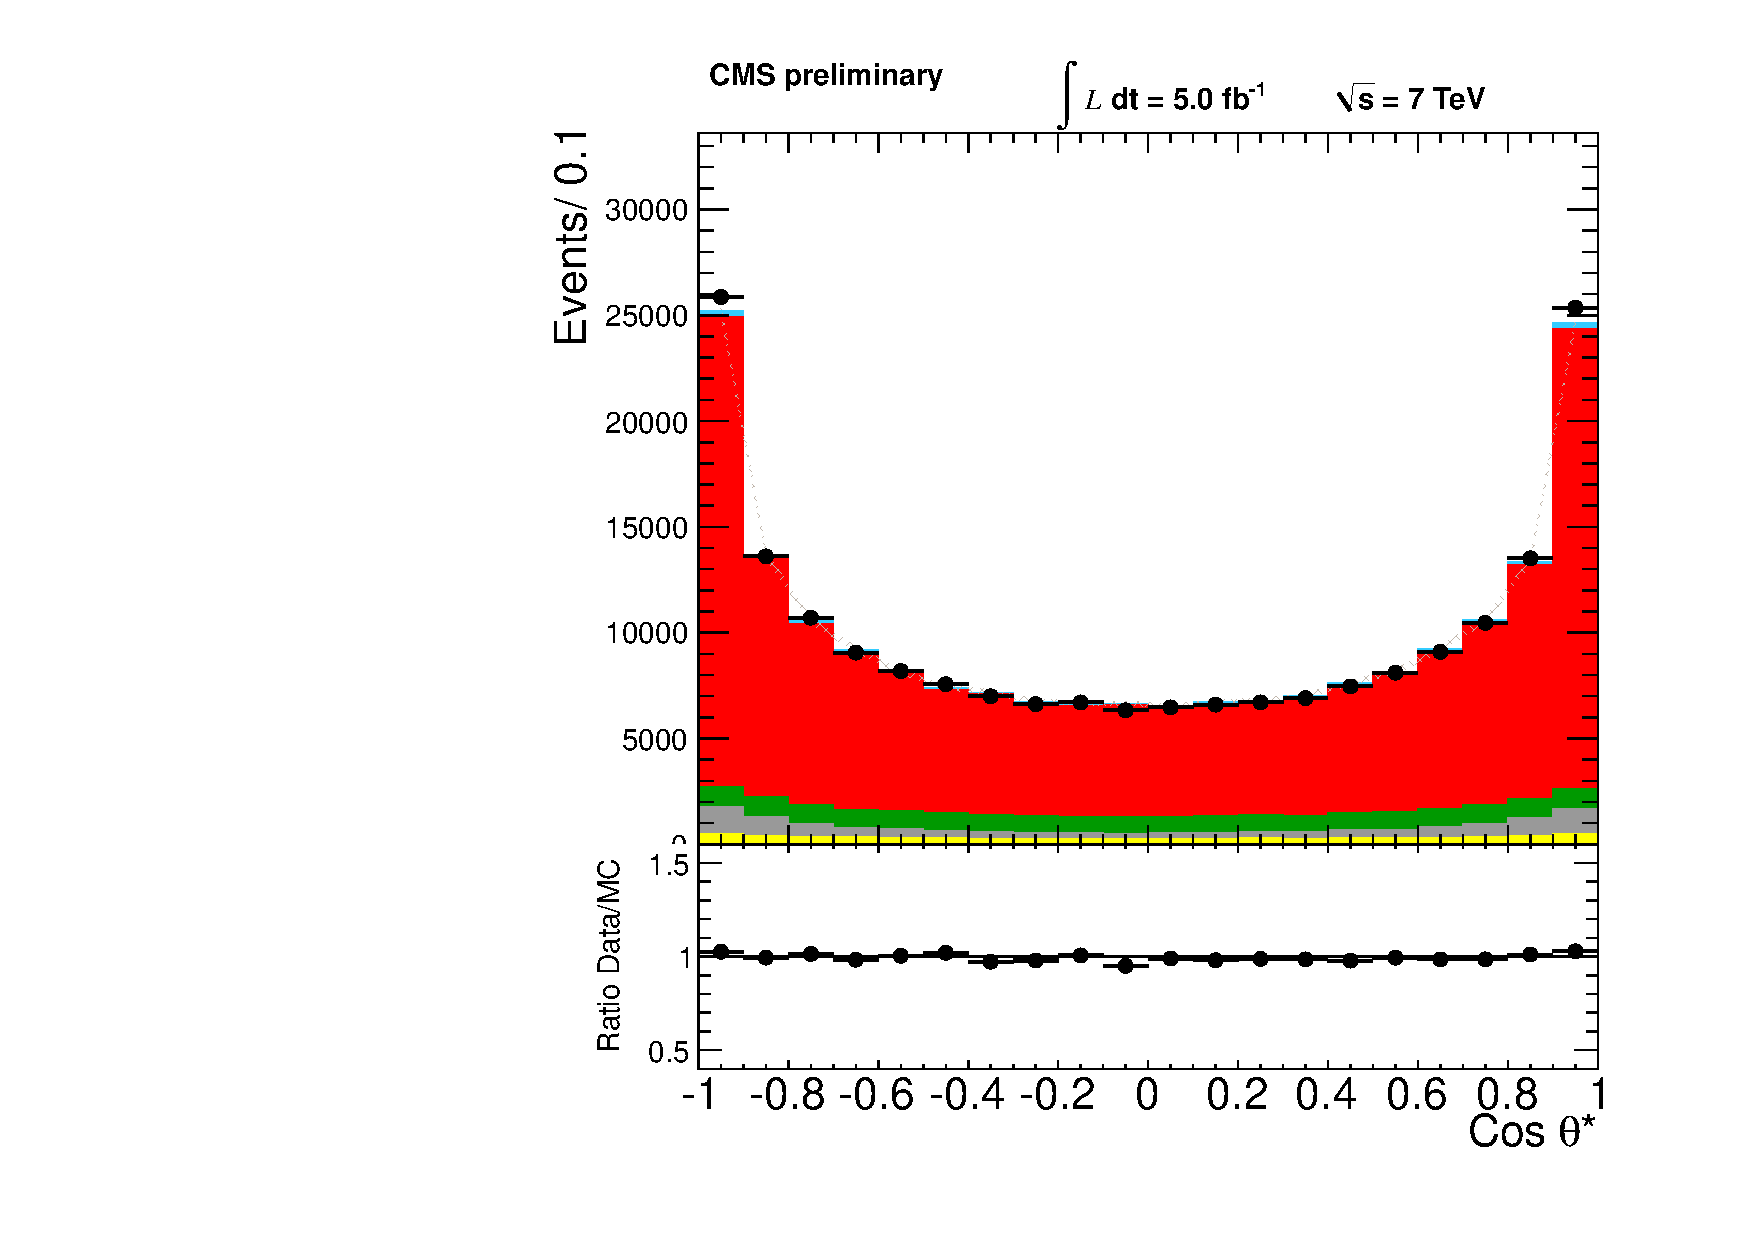
\includegraphics[width=0.49\textwidth]{figs/n-1_plots_el/el_hs.pdf}
    \caption{Comparison of the angular distributions for $\cos\theta^{\ast}$ from data and MC 
   for the electron+jets selection.}
\label{fig:elec_thetas}}
\end{figure}
%%%%%%%%%%%%%%%%%%%%%%%%%%%%
\begin{figure}[h!t]
  {\centering
    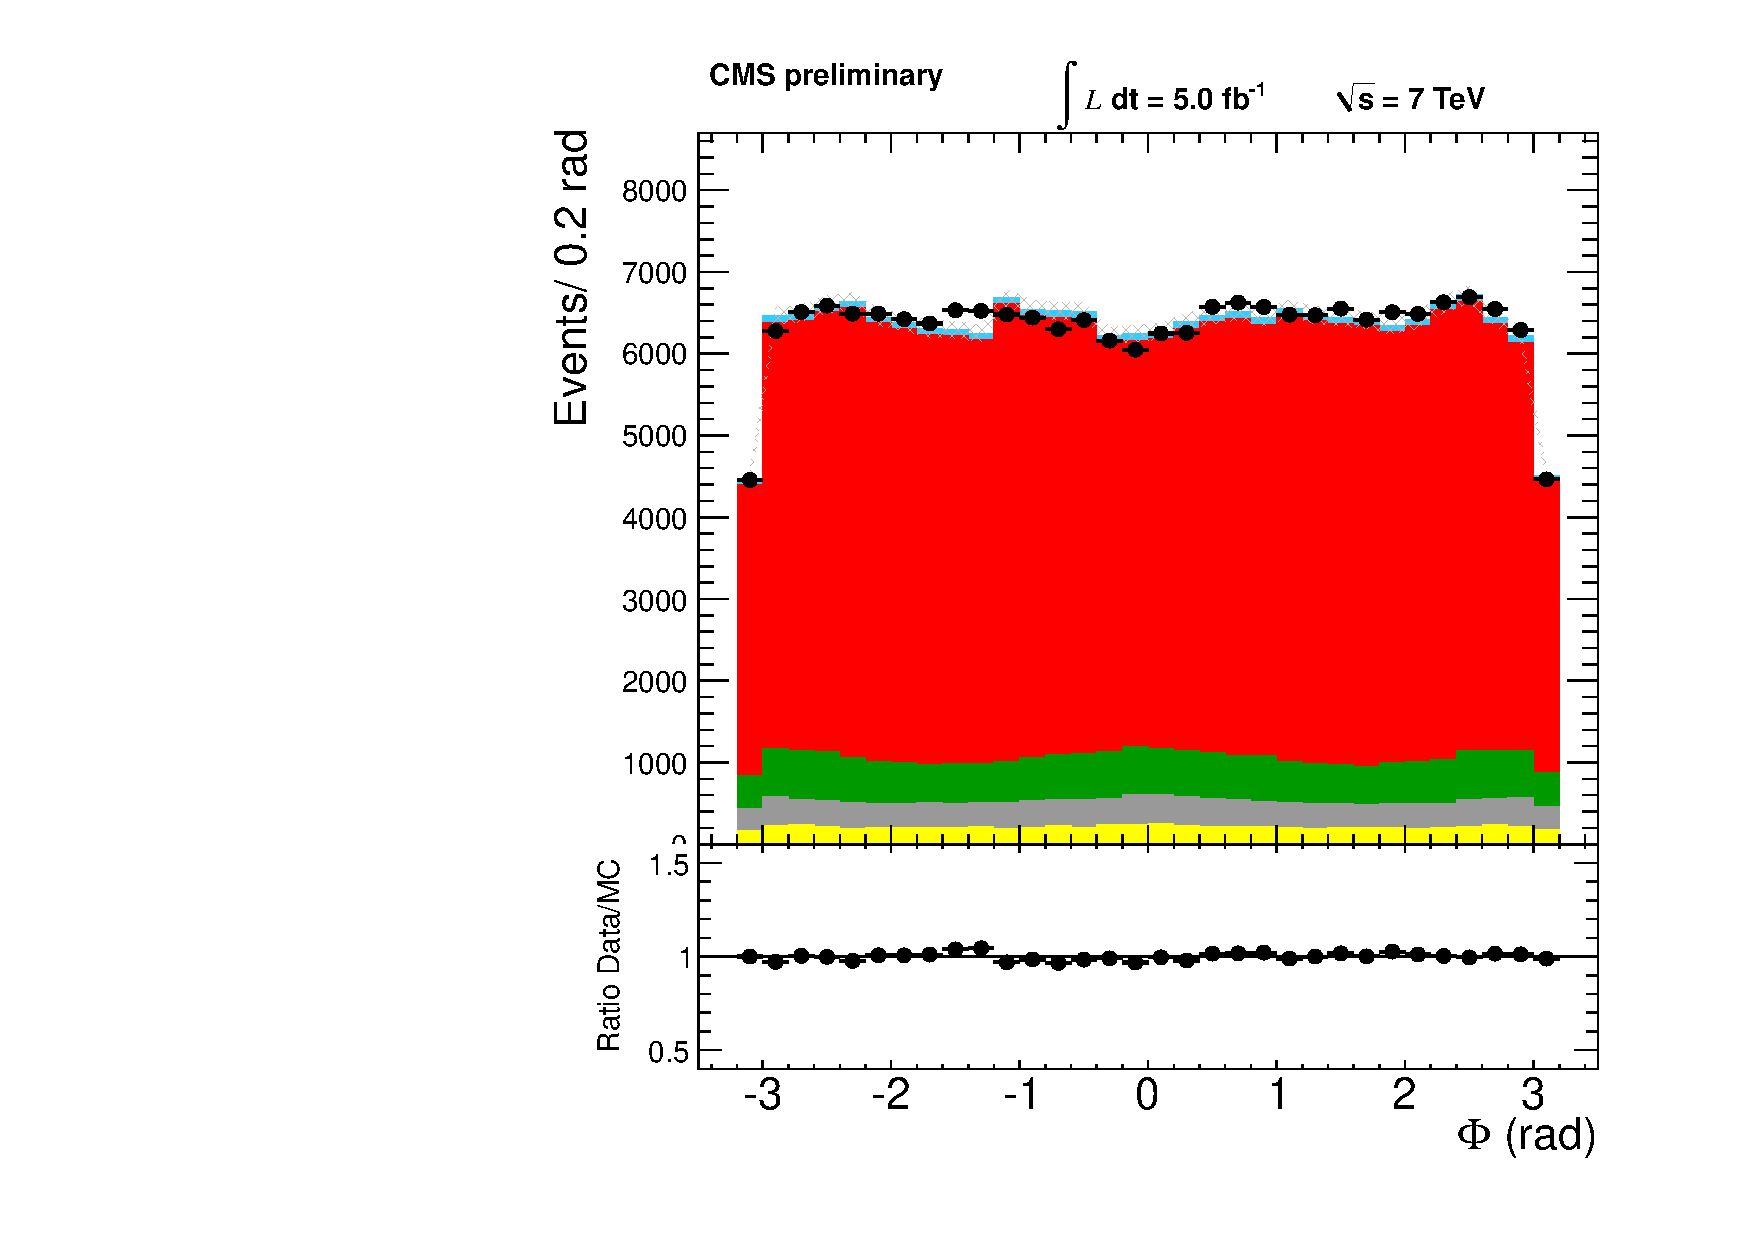
\includegraphics[width=0.49\textwidth]{figs/n-1_plots_el/el_phi.pdf}
    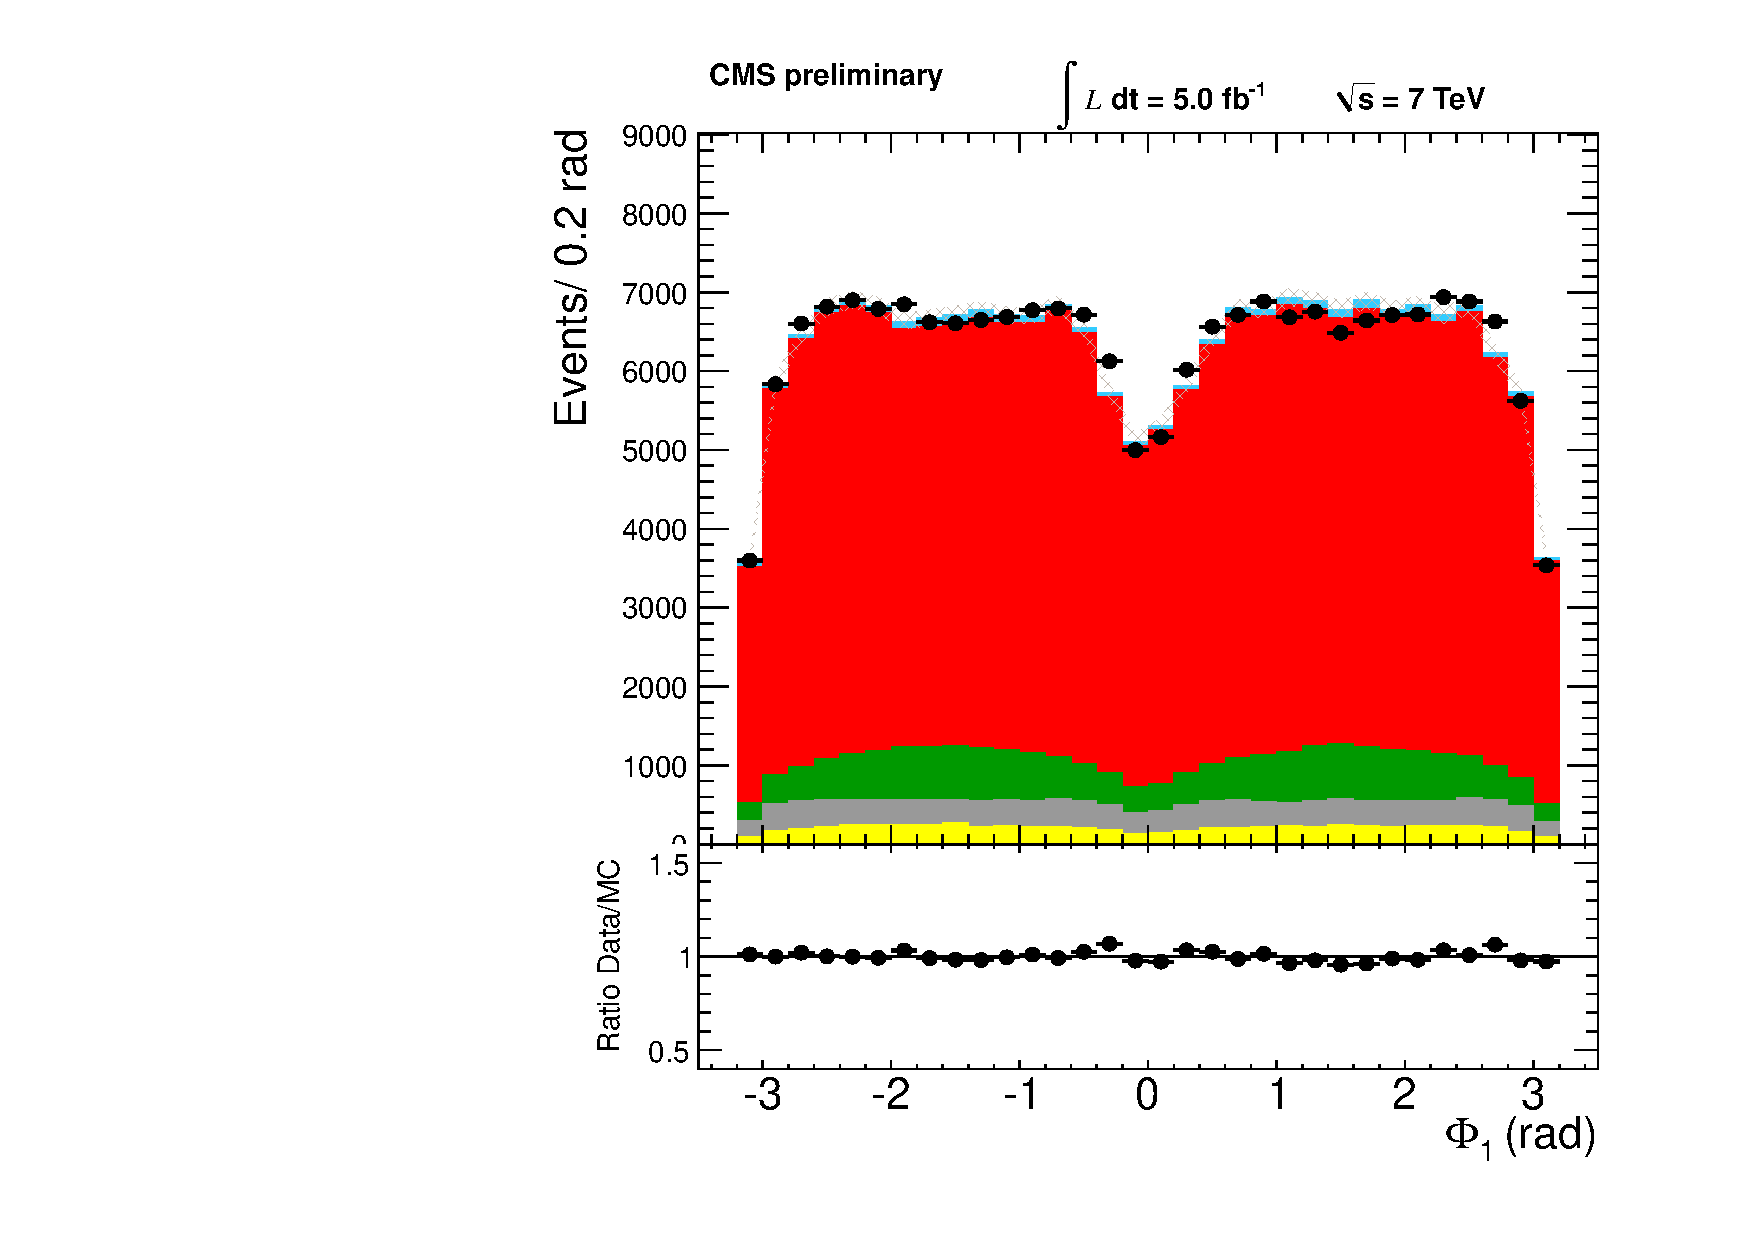
\includegraphics[width=0.49\textwidth]{figs/n-1_plots_el/el_phib.pdf}
    \caption{Comparison of the angular distributions for $\Phi$  (left)
    $\Phi_{1}$ (right) from data and MC for the 
    electron+jets selection.}
\label{fig:elec_phi}}
\end{figure}

%%%%%%%%%%%%%%%%%%%%%%%%%%%%
\begin{figure}[h!t]
  {\centering
    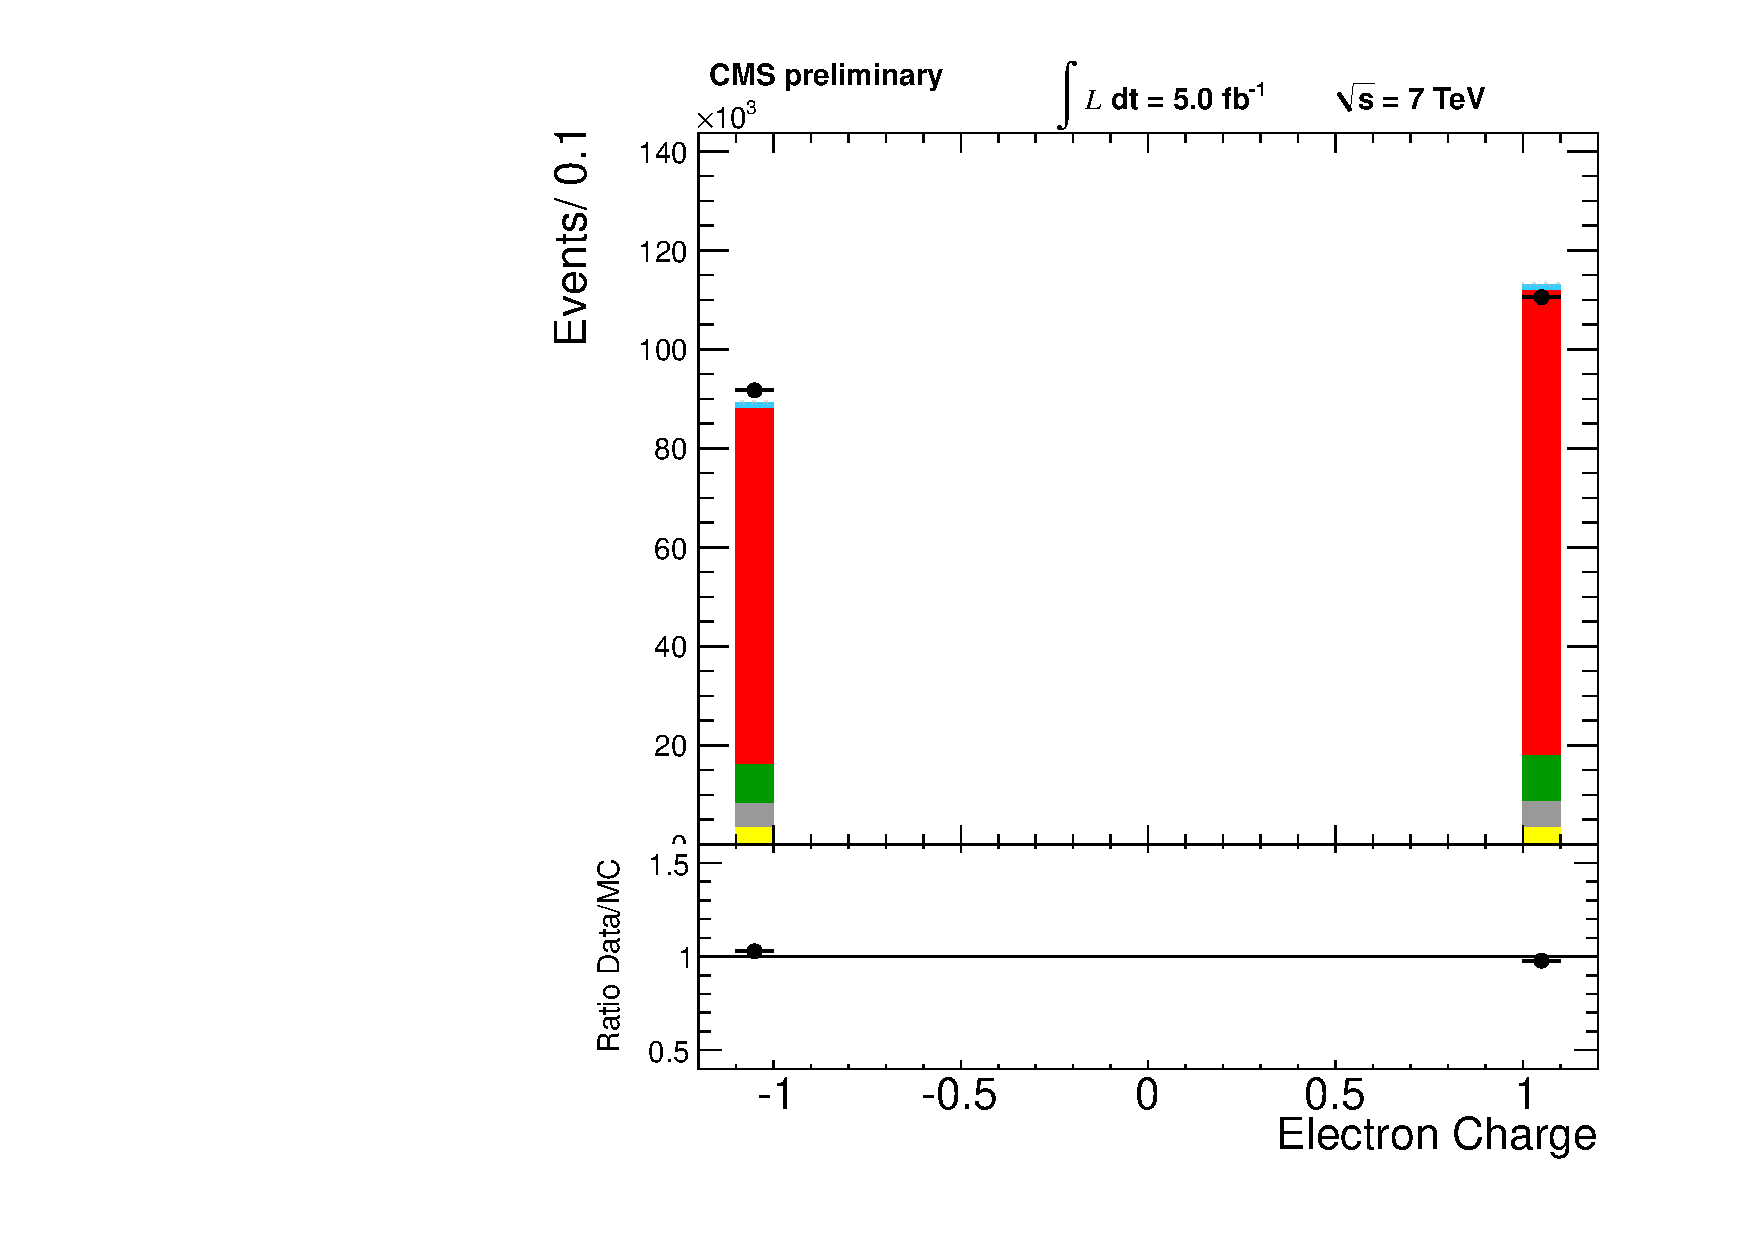
\includegraphics[width=0.49\textwidth]{figs/n-1_plots_el/el_charge.pdf}
    \caption{Comparison of the charge of the electron from data and MC for the electron+jets selection.}
\label{fig:elec_chg}}
\end{figure}

% rapidity and pt of the WW system

%%%%%%%%%%%%%%%%%%%%%%%%%%%%
\begin{figure}[h!t]
  {\centering
    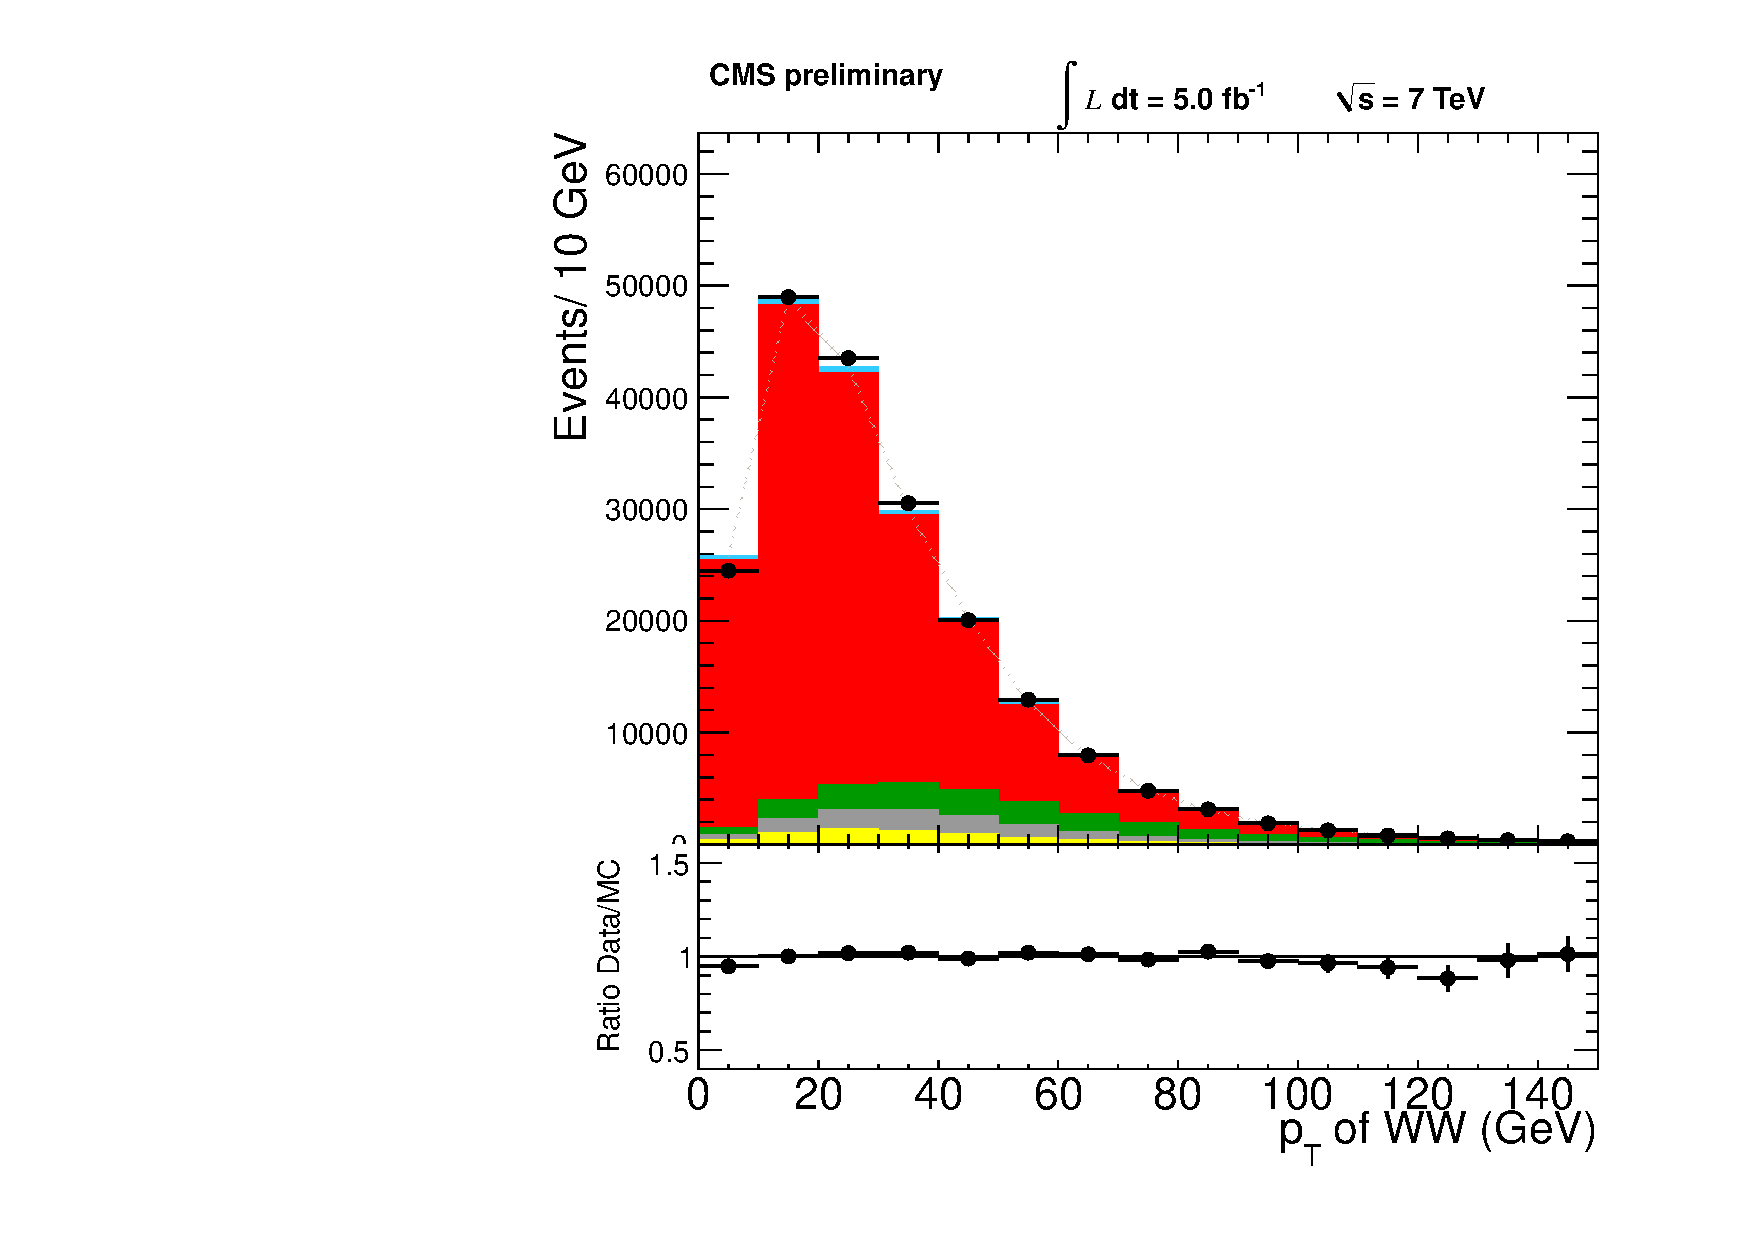
\includegraphics[width=0.49\textwidth]{figs/n-1_plots_el/el_ptlvjj.pdf}
    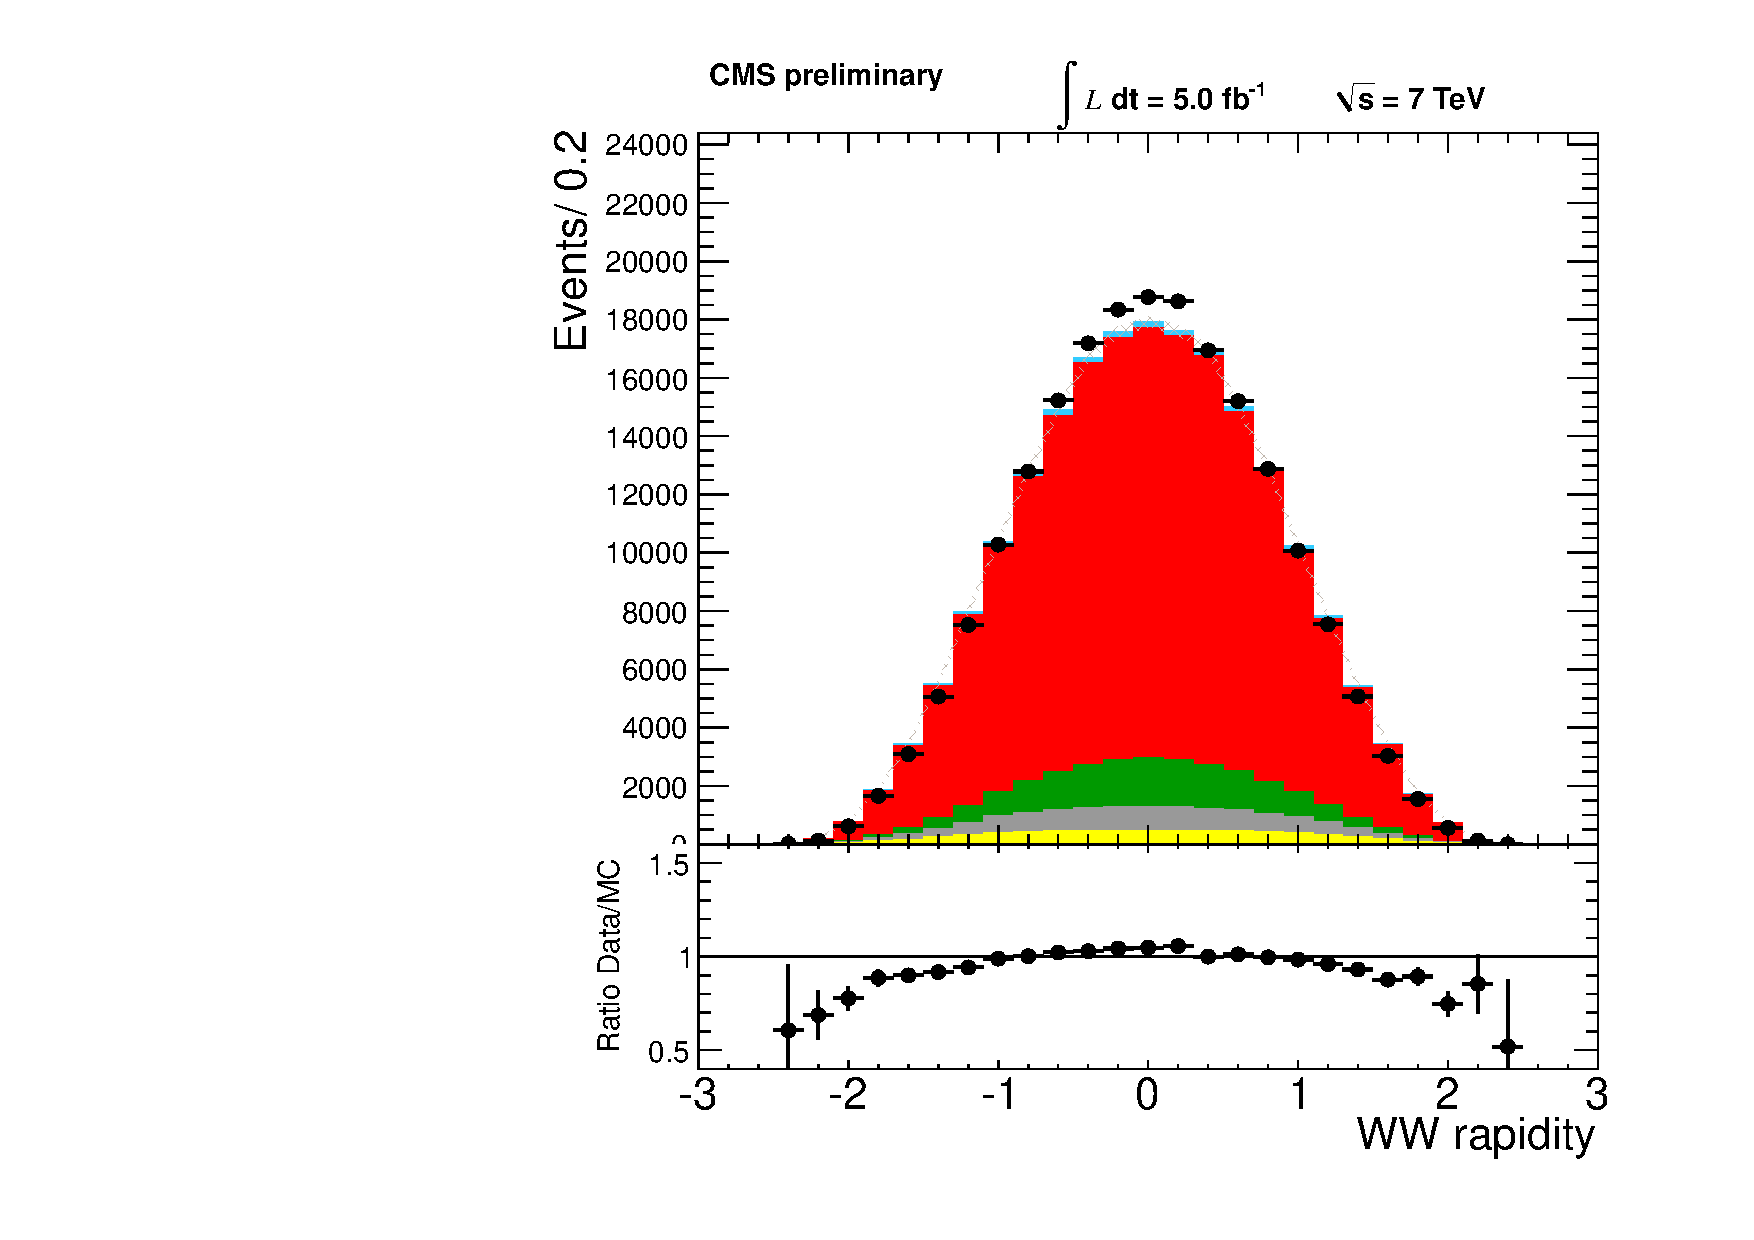
\includegraphics[width=0.49\textwidth]{figs/n-1_plots_el/el_etalvjj.pdf}
    \caption{Comparison of the $p_{T}$ (left) $\eta$ (right) of the WW system
      from data and MC for the electron+jets selection.}
\label{fig:elec_ww}}
\end{figure}

%%%%%%%%%%%%%%%%%%%%%%%%%%%%
\begin{figure}[h!t]
  {\centering
    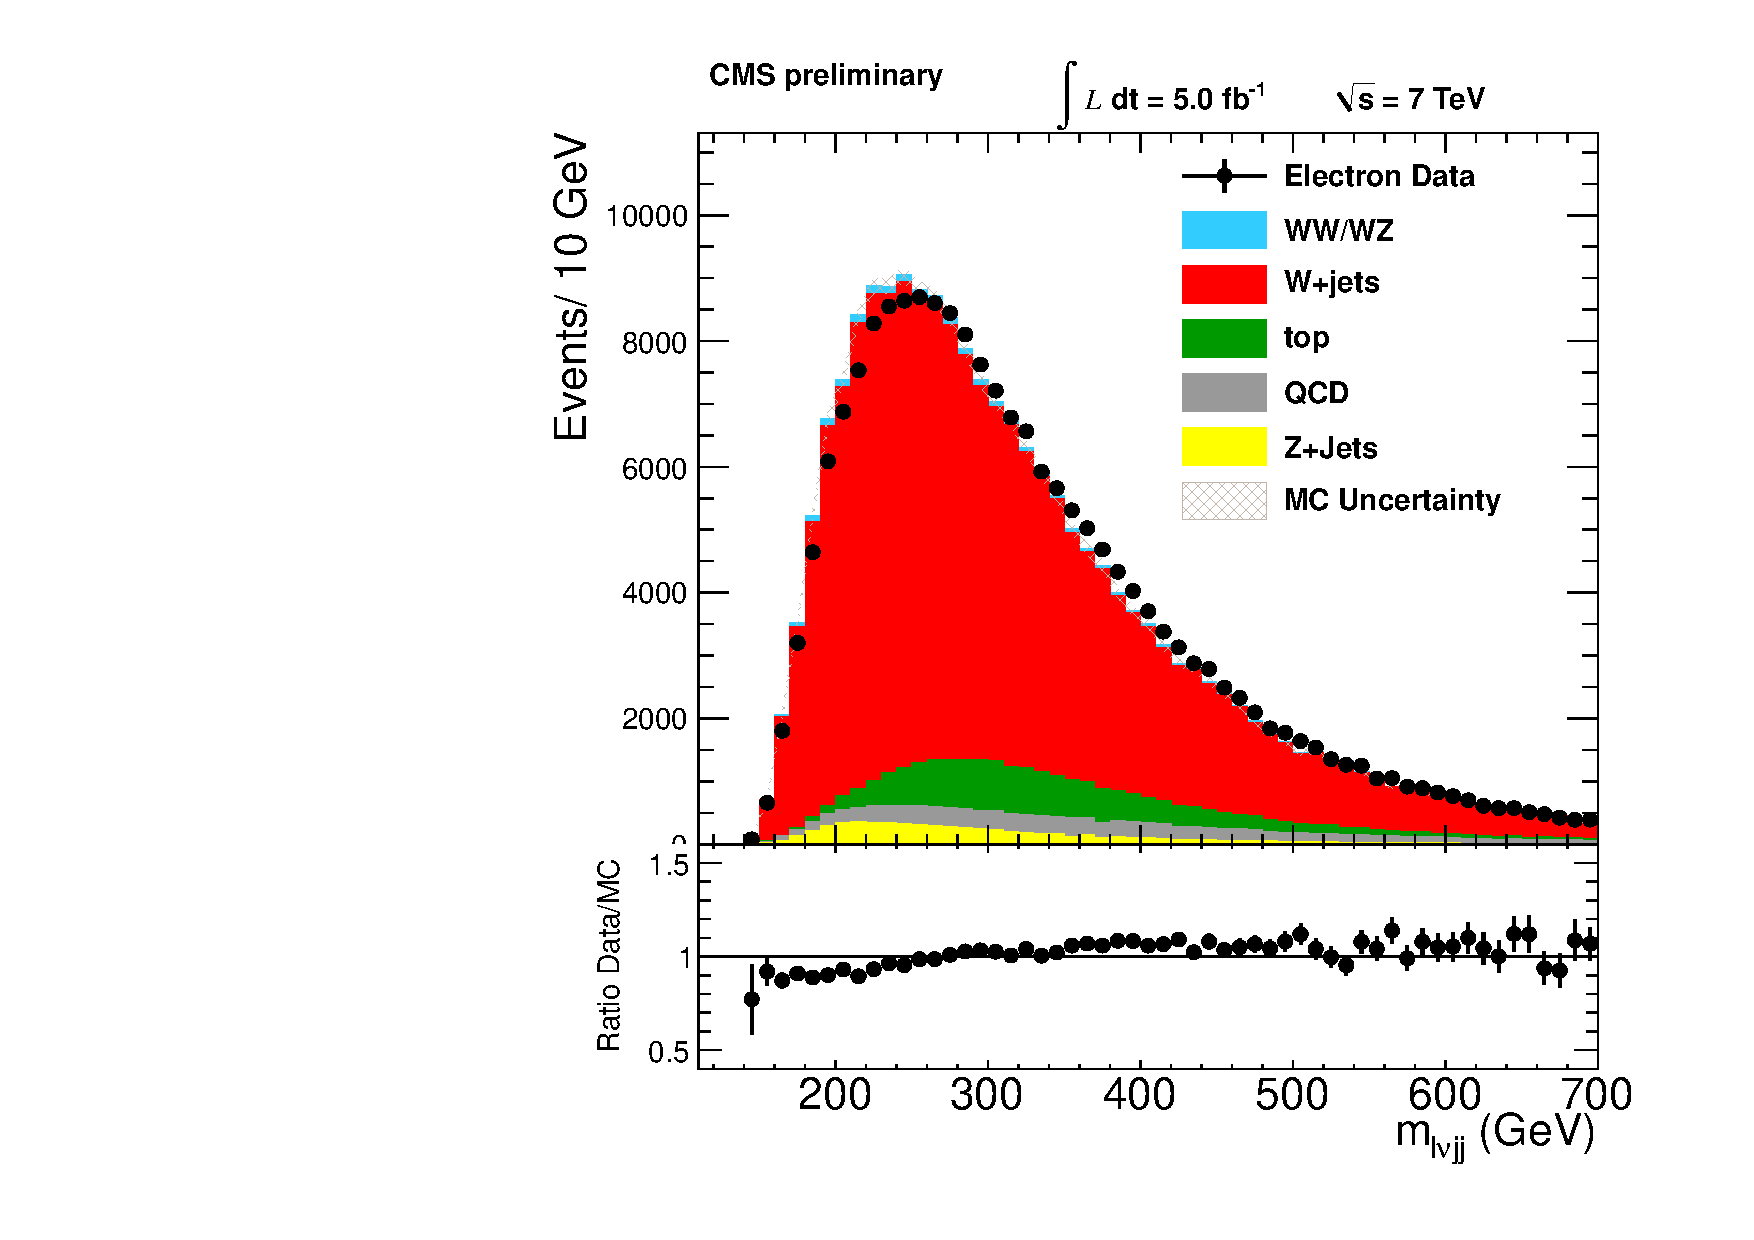
\includegraphics[width=0.49\textwidth]{figs/n-1_plots_el/el_mlvjj.pdf}
    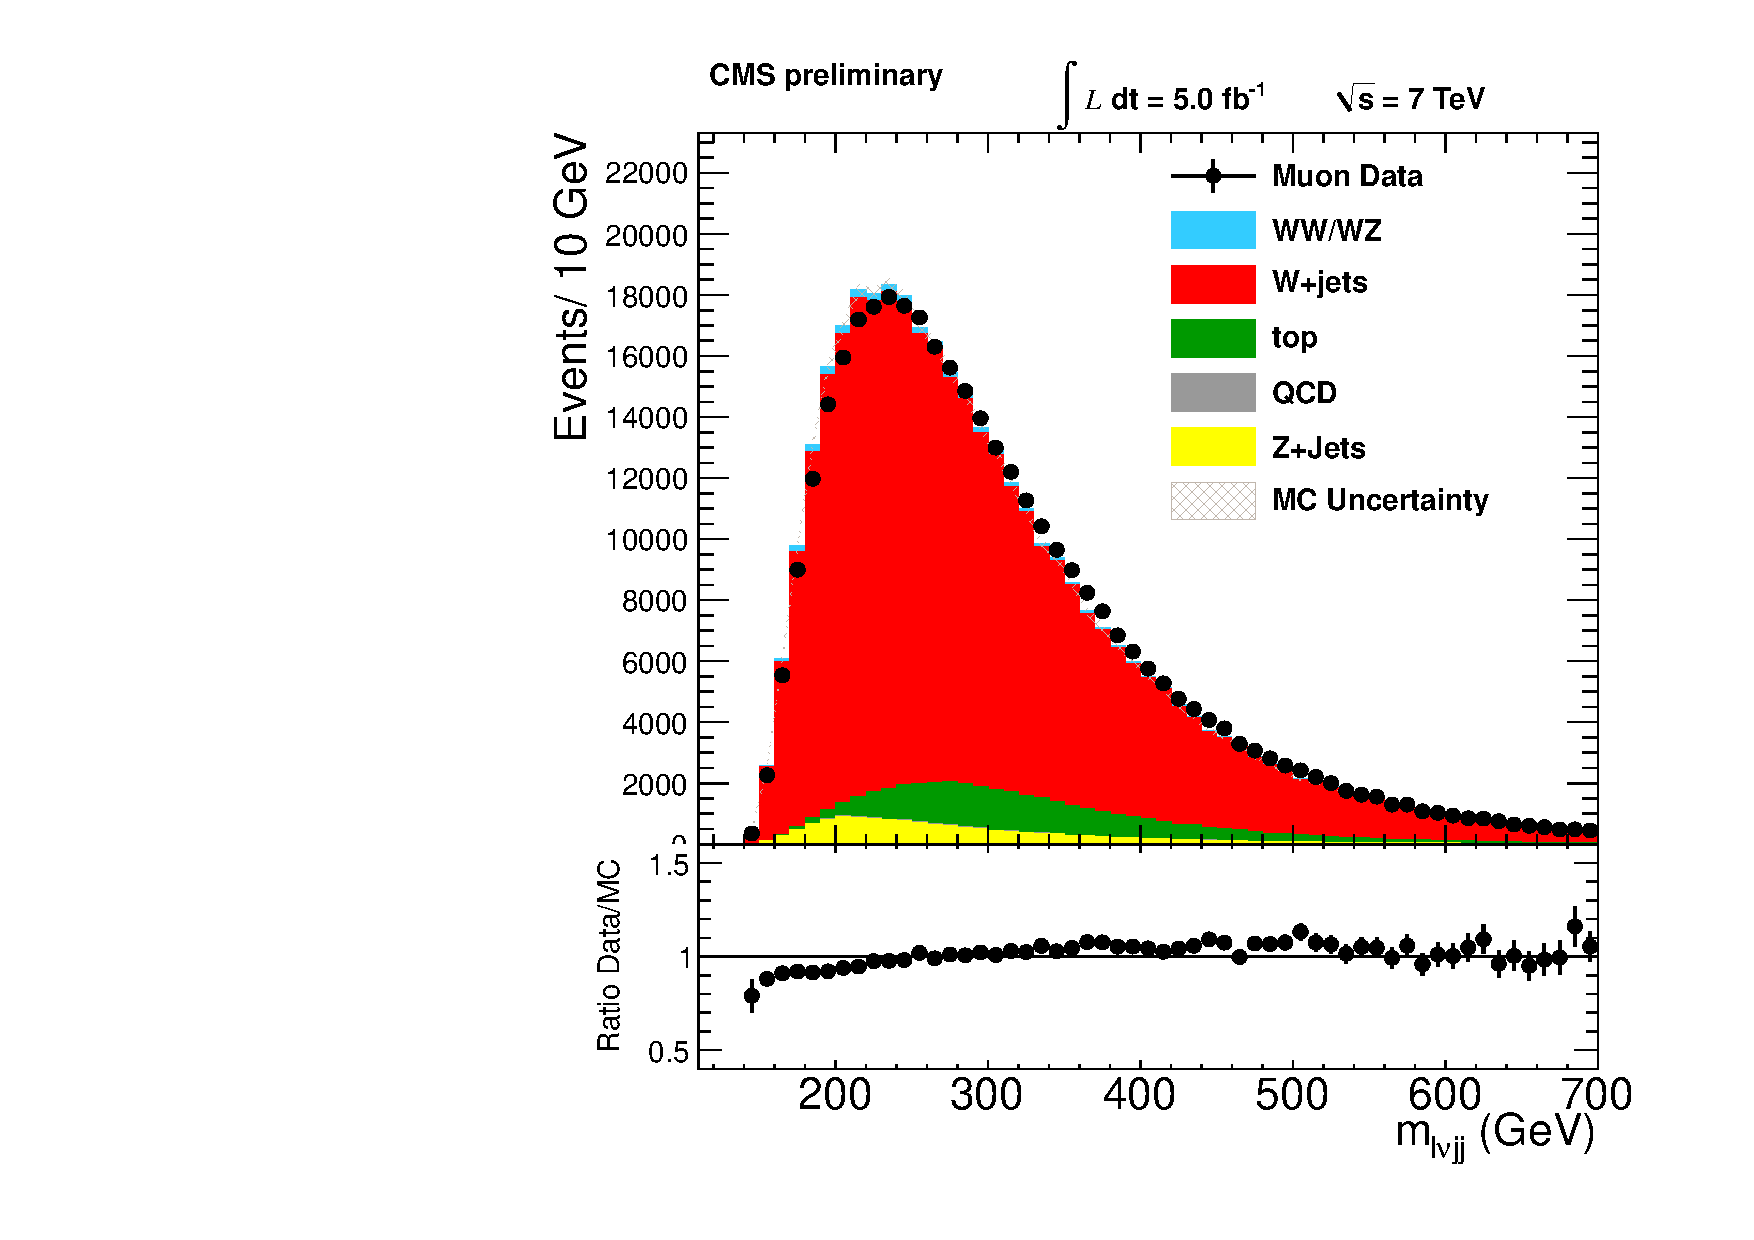
\includegraphics[width=0.49\textwidth]{figs/n-1_plots_mu/mu_mlvjj.pdf}
    \caption{Comparison of the four-body invariant mass from data and MC for the electron+jets selection (left) 
             and muon+jets selection (right).}
\label{fig:lep_mlvjj}}
\end{figure}

%%%%%%%%%%%%%%%%%%%%%%%%%%%%%%%%%
%%%%%%%%%%%%%%%%%%%%%%%
\clearpage

\subsection{Data MC comparison in the \texorpdfstring{$t\bar{t}$}{ttbar} control sample}
The data MC comparison for the various inputs to the MVA for the  $t\bar{t}$ control 
sample are shown in  
Figures ~\ref{fig:mu_ttbar_jet_qgl}-\ref{fig:mu_ttbar_ww}
for the muon+jets sample and in 
Figures ~\ref{fig:elec_ttbar_jet_qgl}-\ref{fig:elec_ttbar_ww} for
the electron+jets sample. We see that for all the mva input variables data 
agrees well with the MC in the  $t\bar{t}$ control sample.

% quark-gluon discriminants
%%%%%%%%%%%%%%%%%%%%%%%%%%%%
\begin{figure}[h!t]
  {\centering
    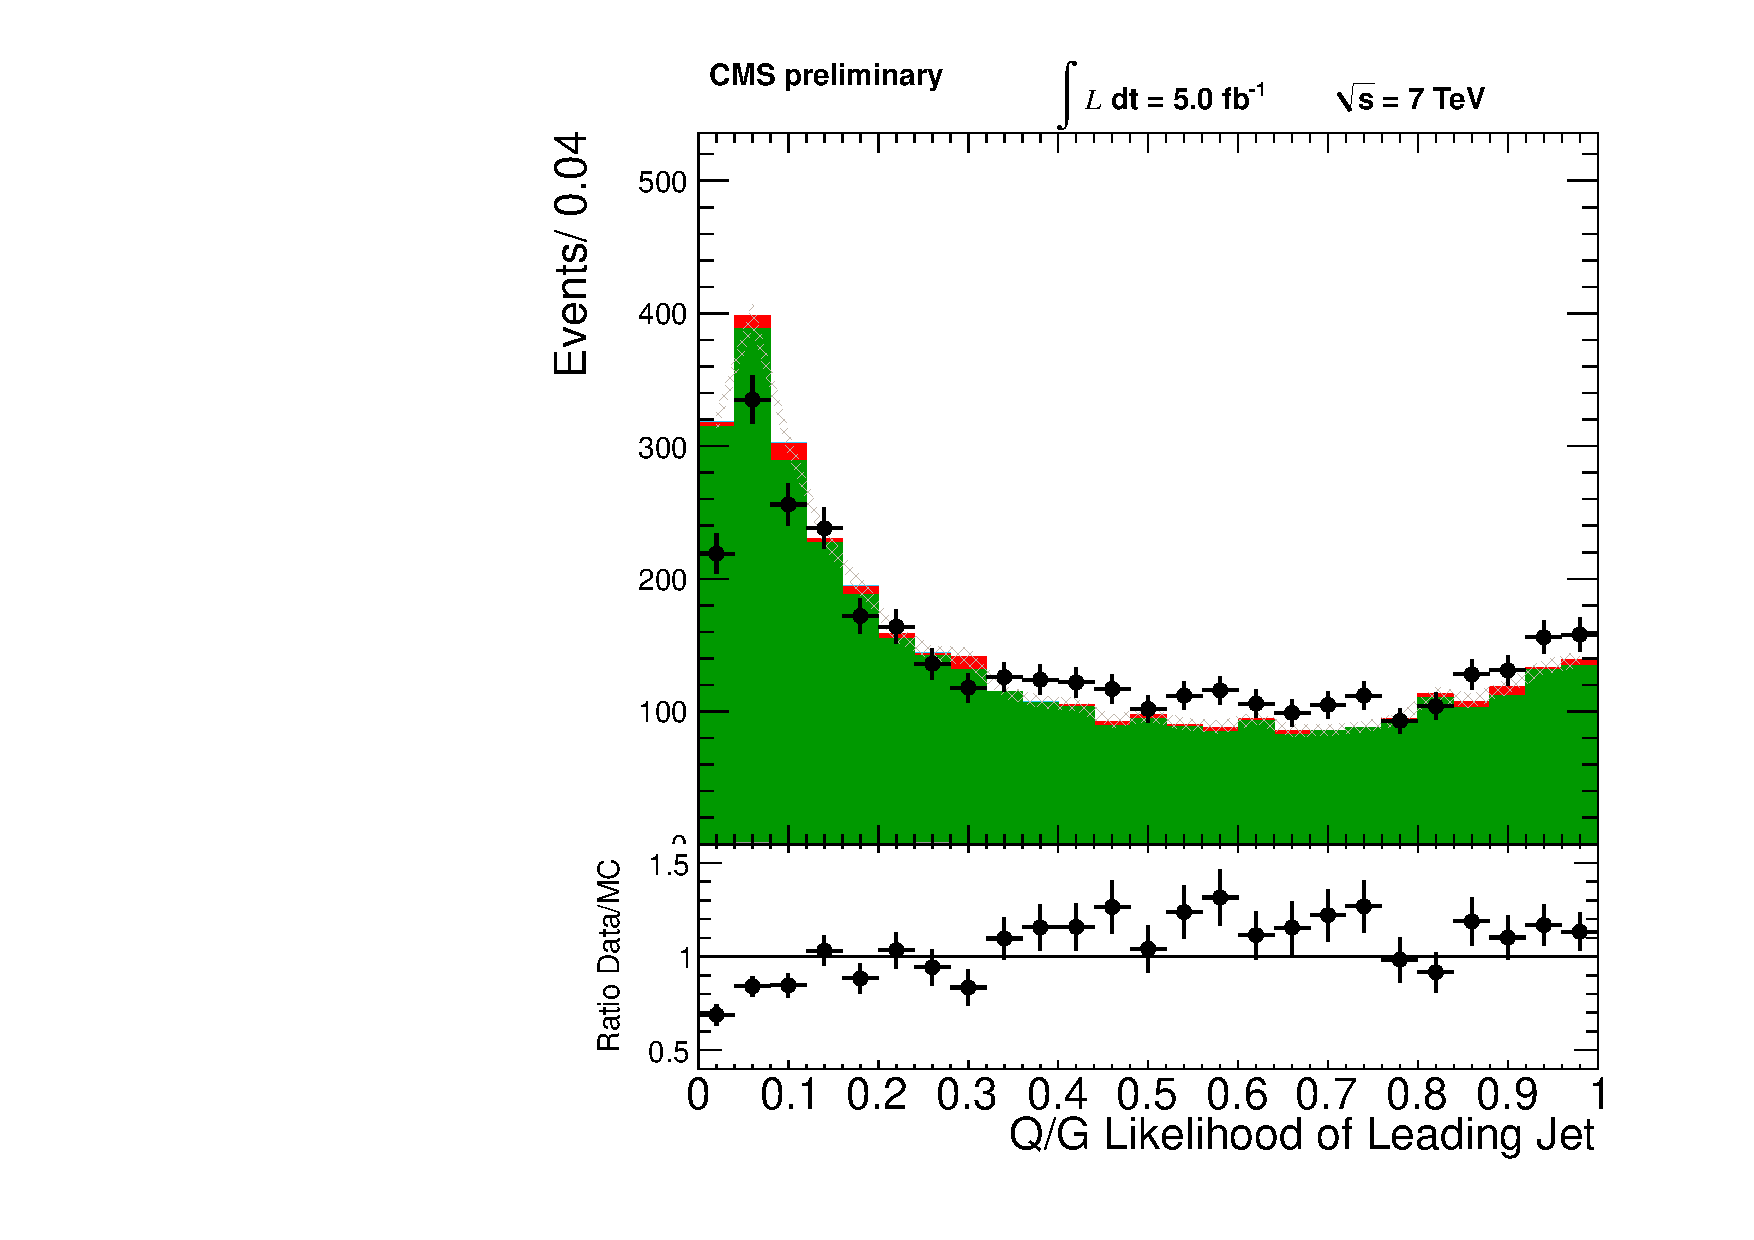
\includegraphics[width=0.49\textwidth]{figs/DataMC_ttbar/mu_jetld_qgl.pdf}
    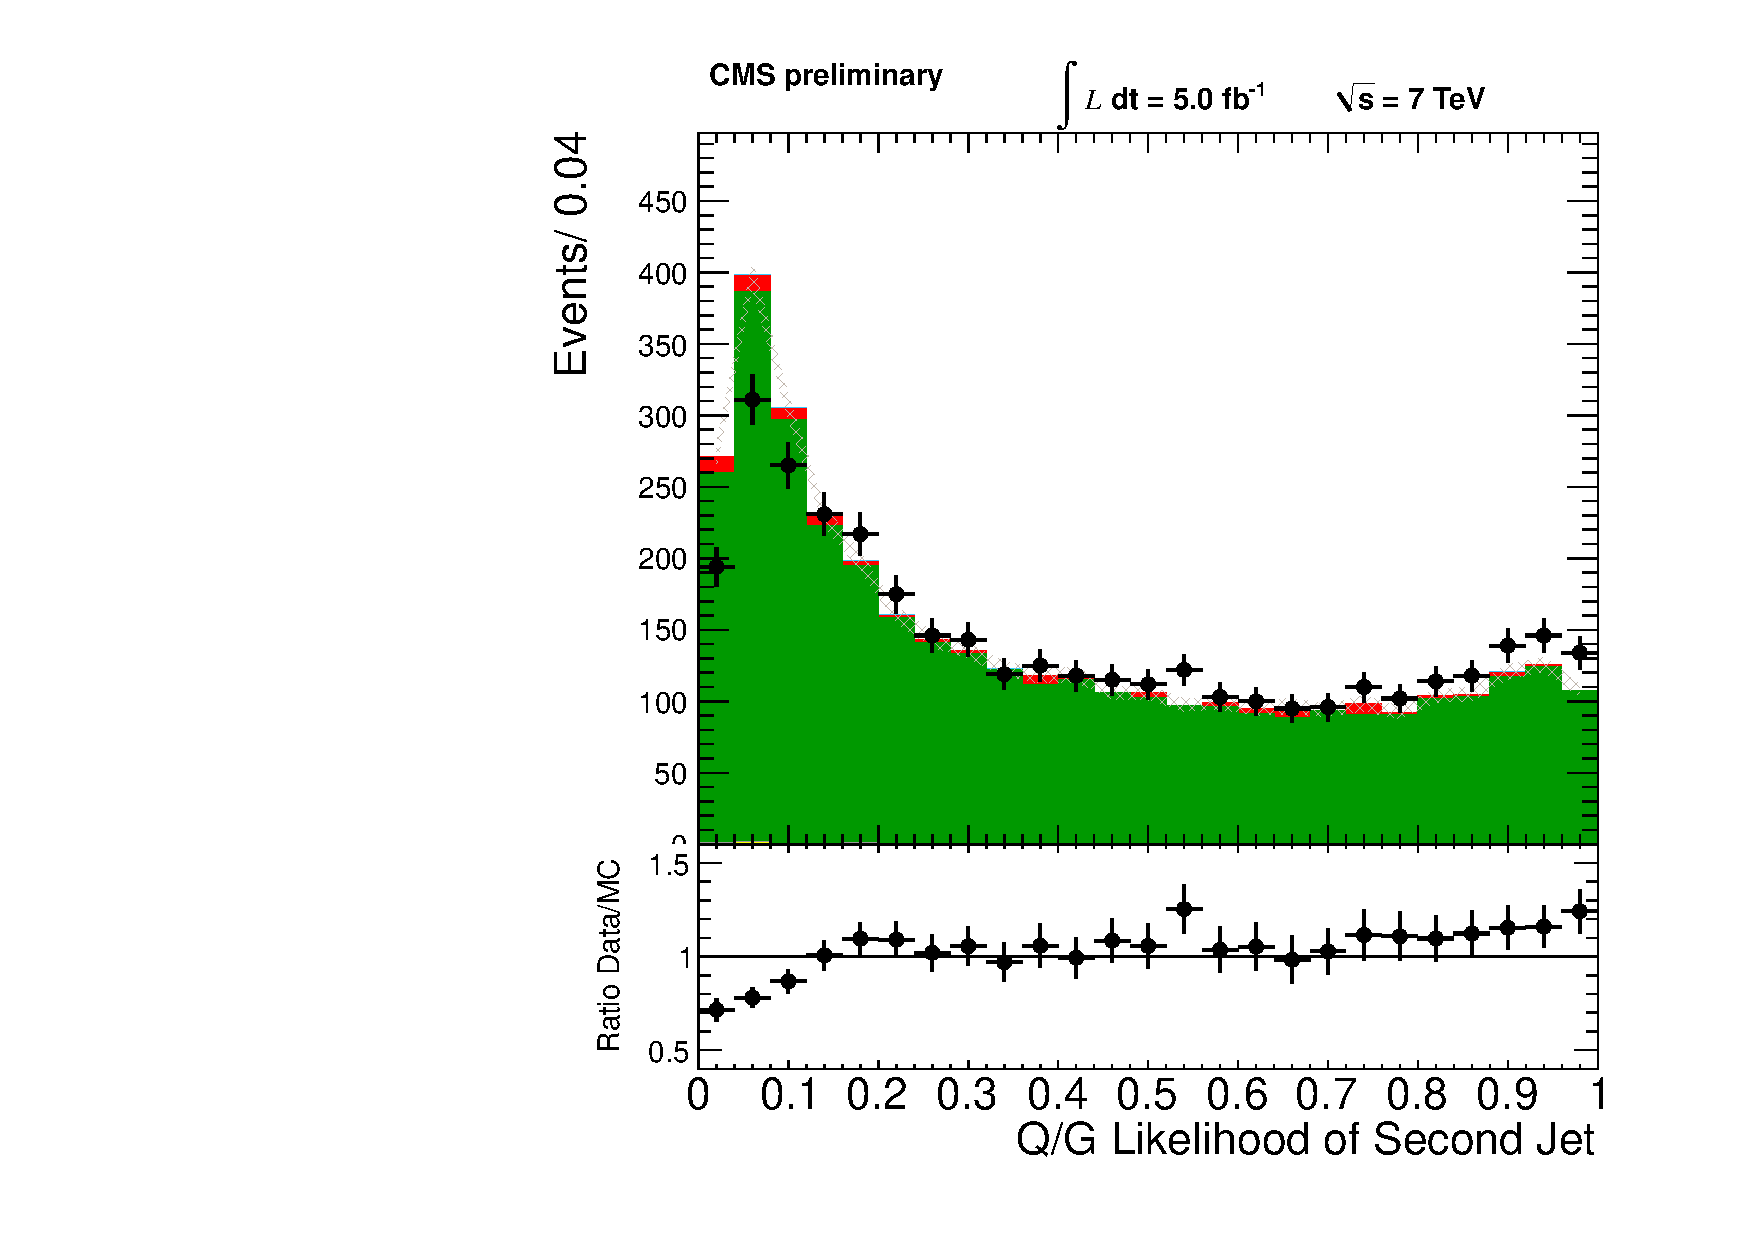
\includegraphics[width=0.49\textwidth]{figs/DataMC_ttbar/mu_jetnt_qgl.pdf}
    \caption{Comparison of the Quark-gluon likelihood distributions for leading jet (left)
    second leading (right) from data and MC for the muon+jets selection.}
\label{fig:mu_ttbar_jet_qgl}}
\end{figure}
% angular variables
%%%%%%%%%%%%%%%%%%%%%%%%%%%%
\begin{figure}[h!t]
  {\centering
    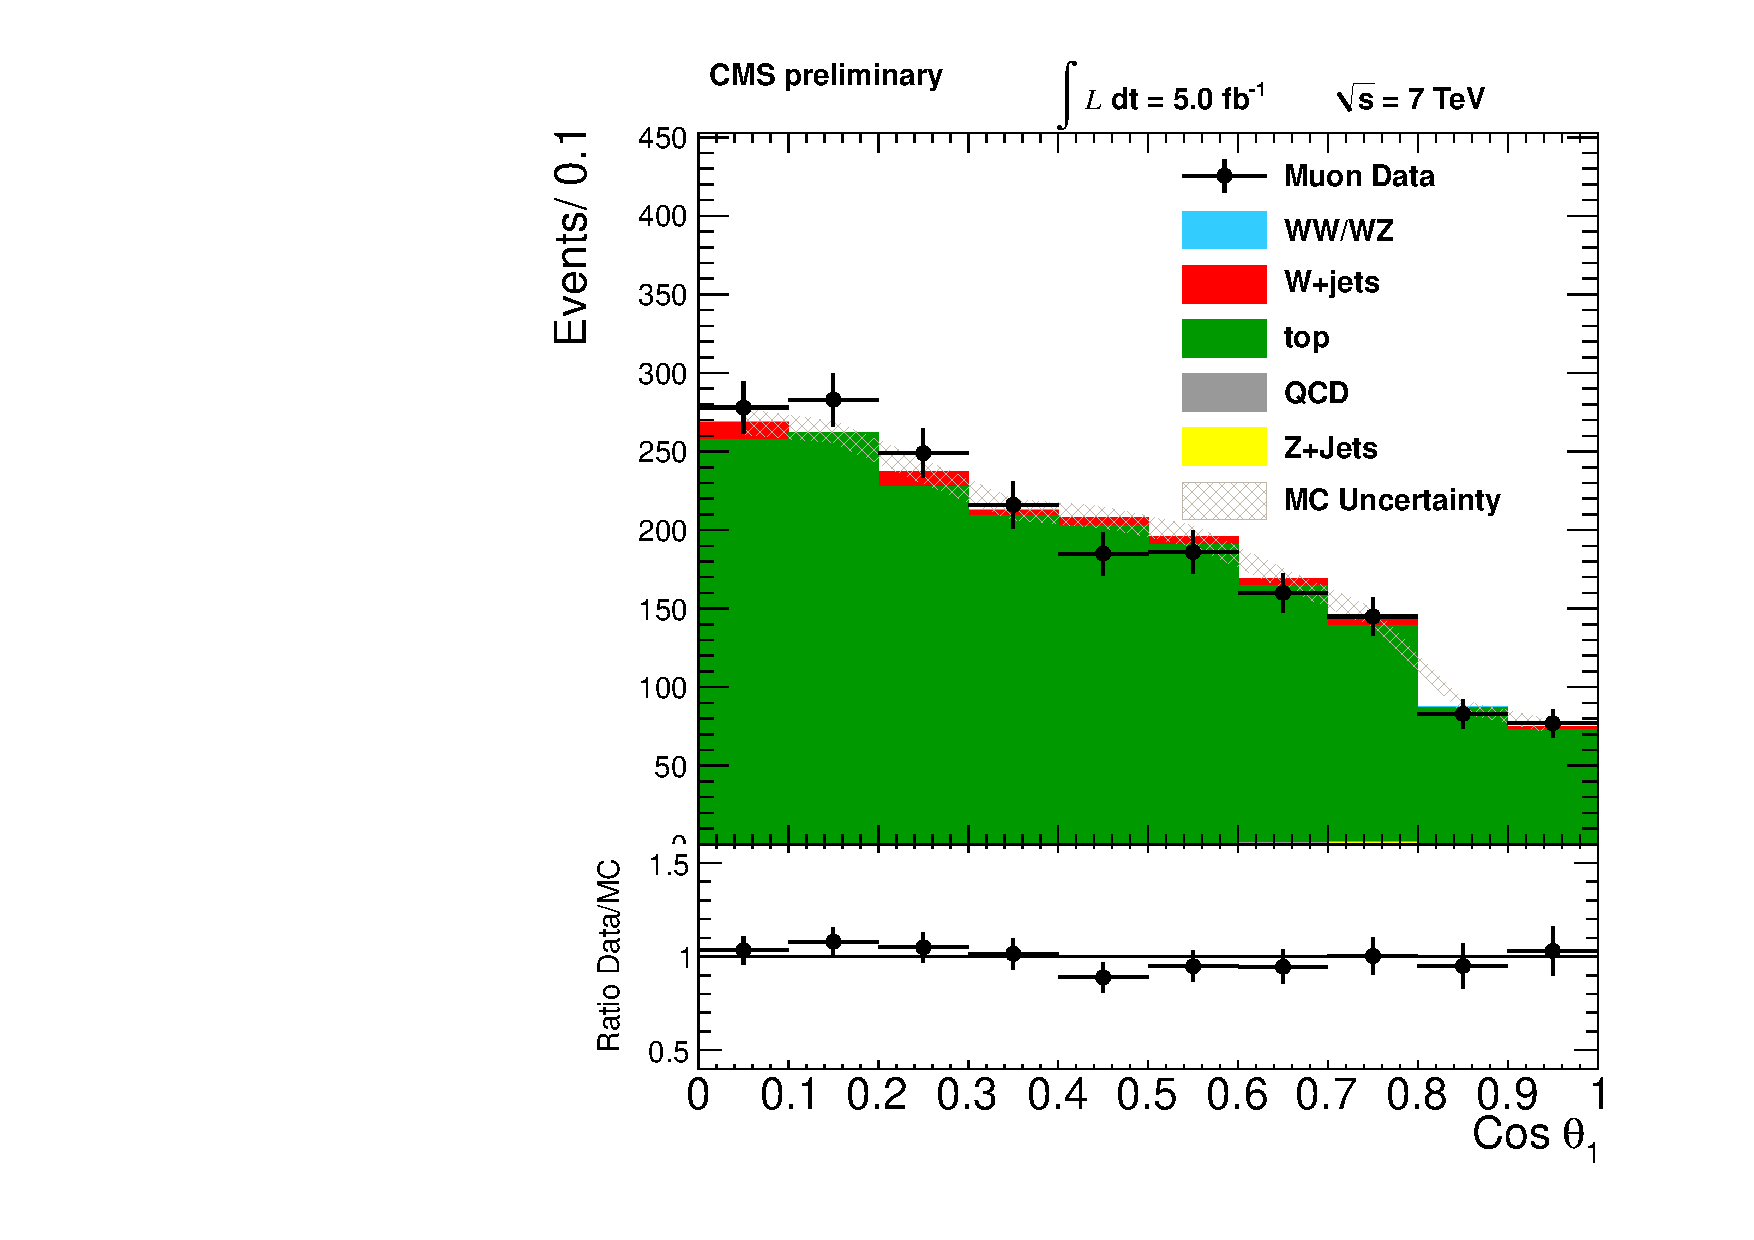
\includegraphics[width=0.49\textwidth]{figs/DataMC_ttbar/mu_ha.pdf}
    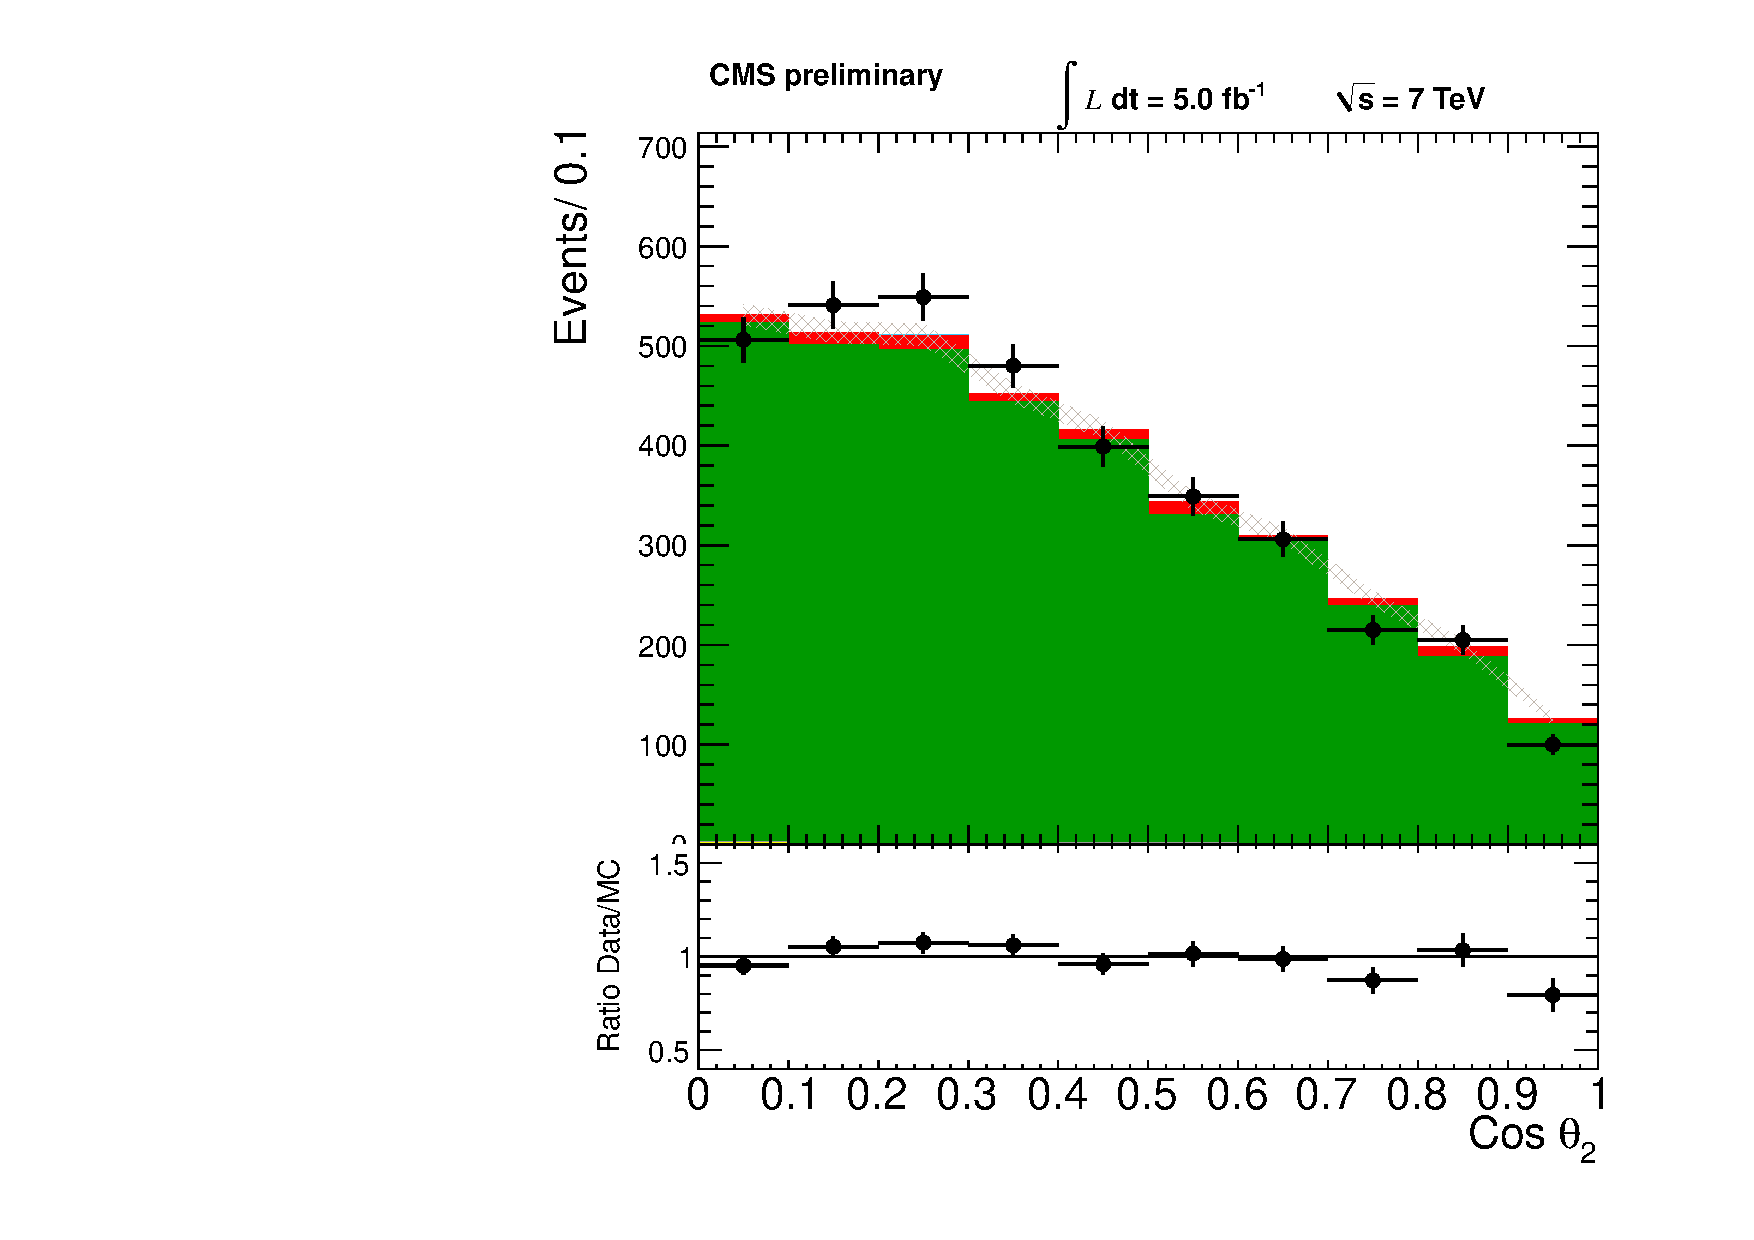
\includegraphics[width=0.49\textwidth]{figs/DataMC_ttbar/mu_hb.pdf}
    \caption{Comparison of the angular distributions for $\cos\theta_{1}$ (left)
   $\cos\theta_{2}$ (right) from data and MC for the muon+jets selection.}
\label{fig:mu_ttbar_theta}}
\end{figure}
%%%%%%%%%%%%%%%%%%%%%%%%%%%%
\begin{figure}[h!t]
  {\centering
     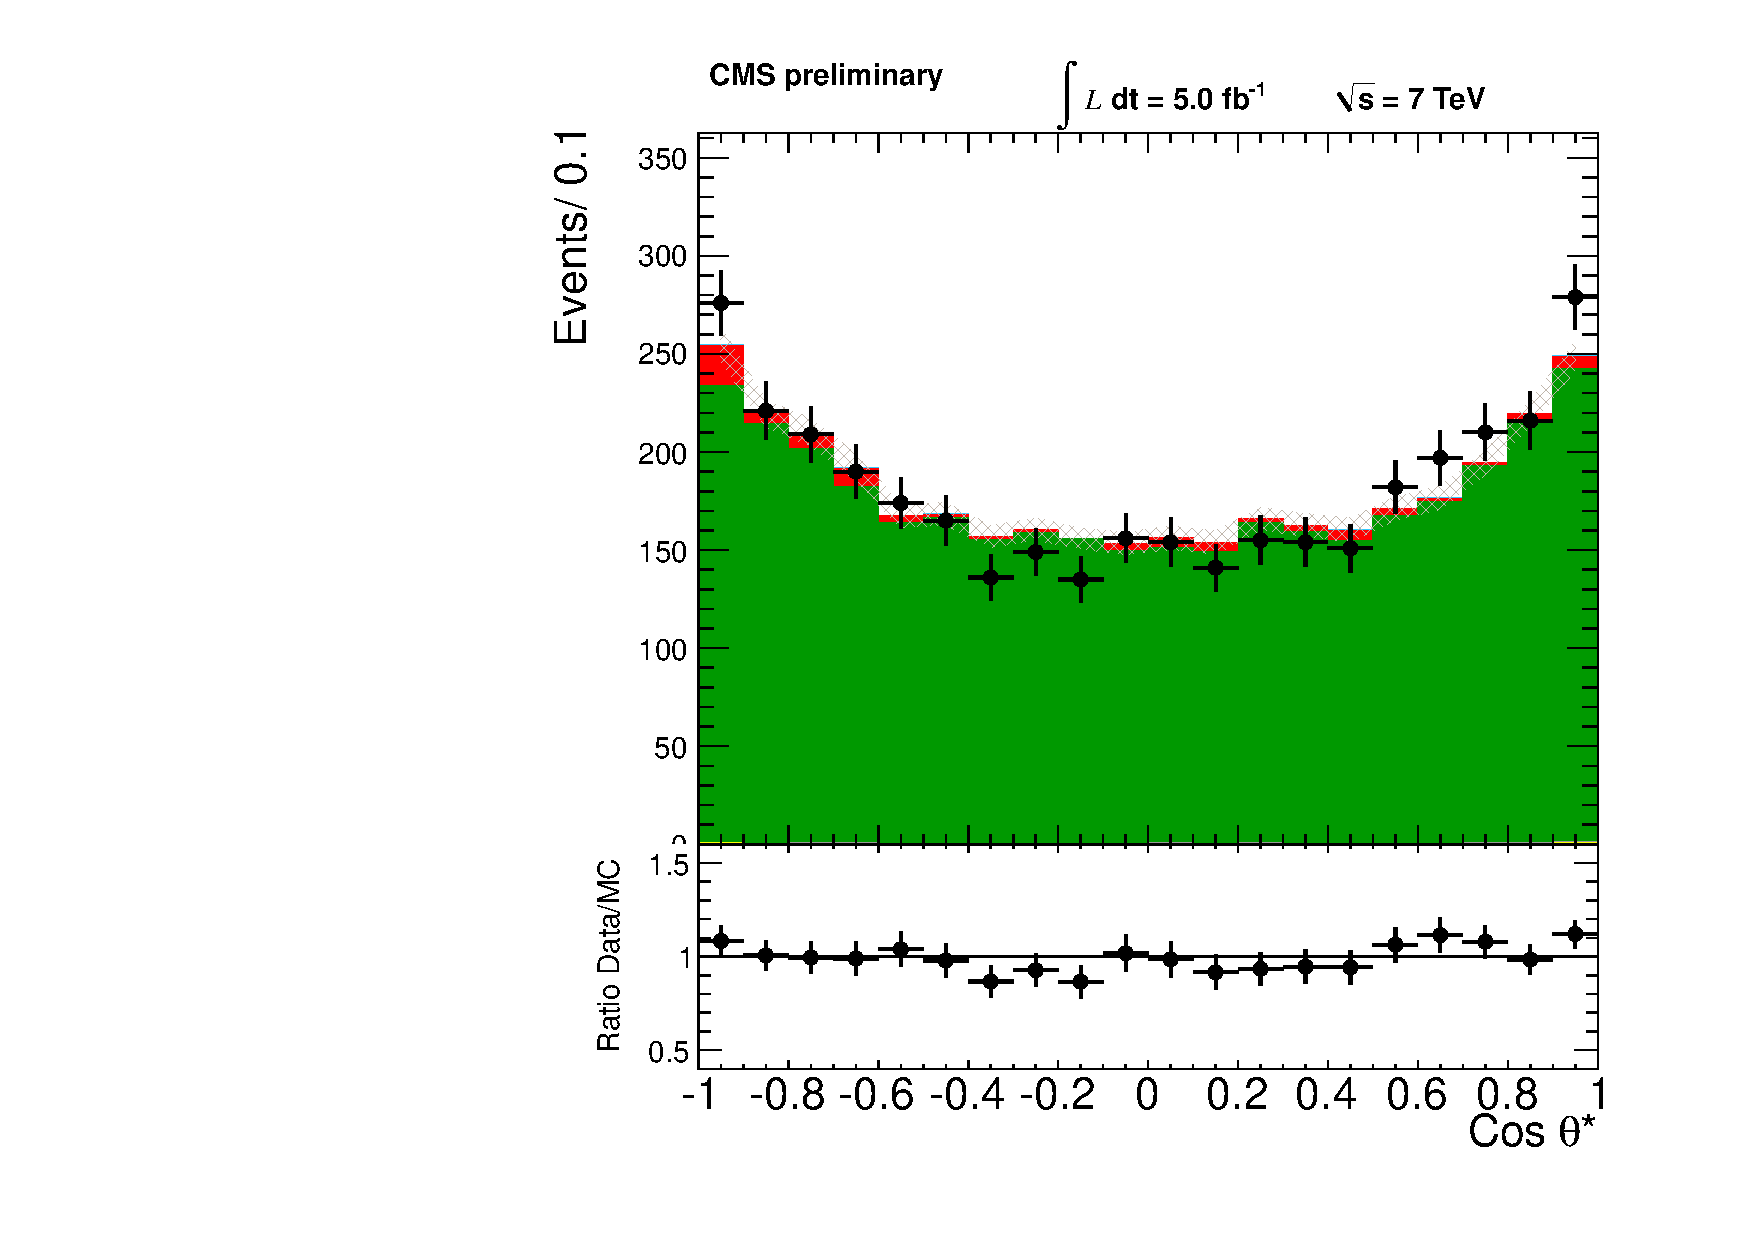
\includegraphics[width=0.49\textwidth]{figs/DataMC_ttbar/mu_hs.pdf}
    \caption{Comparison of the angular distributions for $\cos\theta^{\ast}$ from data and MC 
   for the muon+jets selection.}
\label{fig:mu_ttbar_thetas}}
\end{figure}
%%%%%%%%%%%%%%%%%%%%%%%%%%%%
\begin{figure}[h!t]
  {\centering
    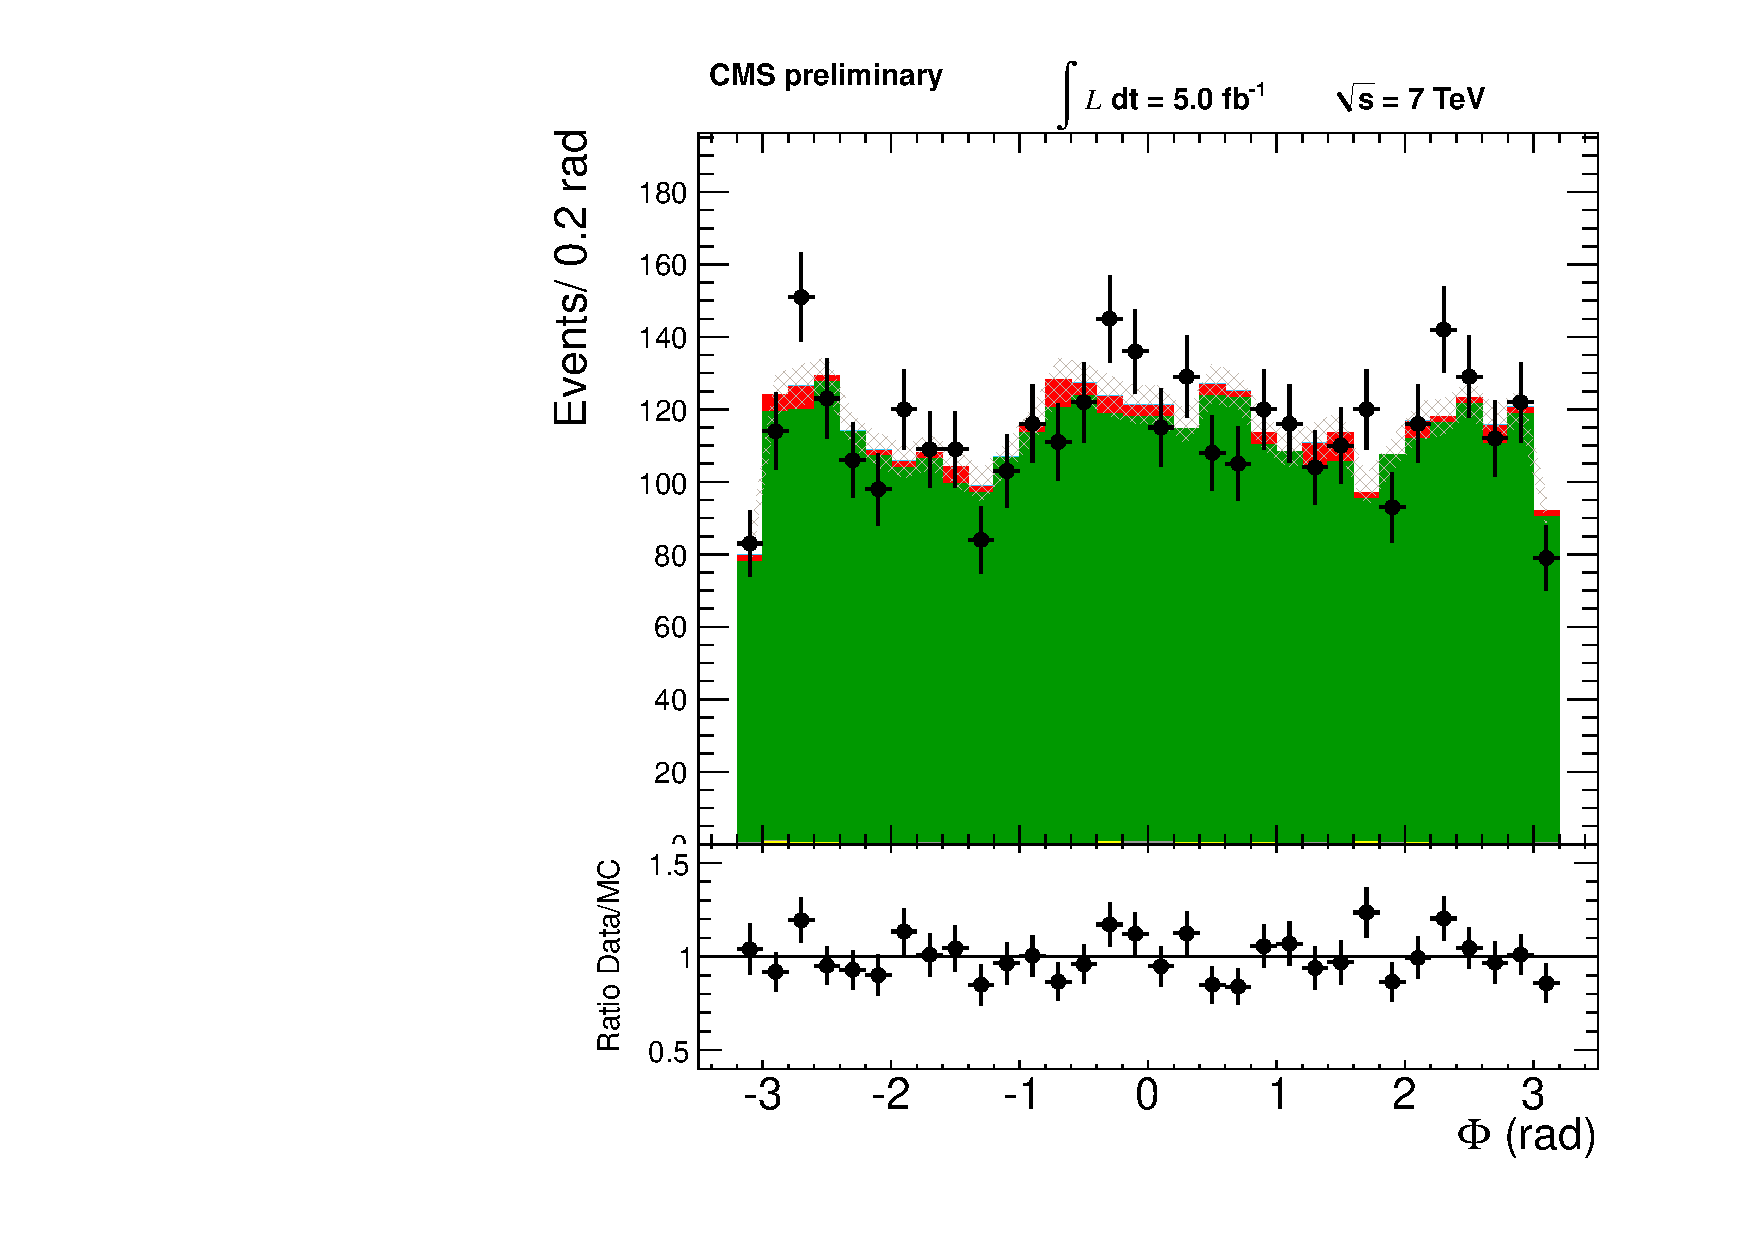
\includegraphics[width=0.49\textwidth]{figs/DataMC_ttbar/mu_phi.pdf}
    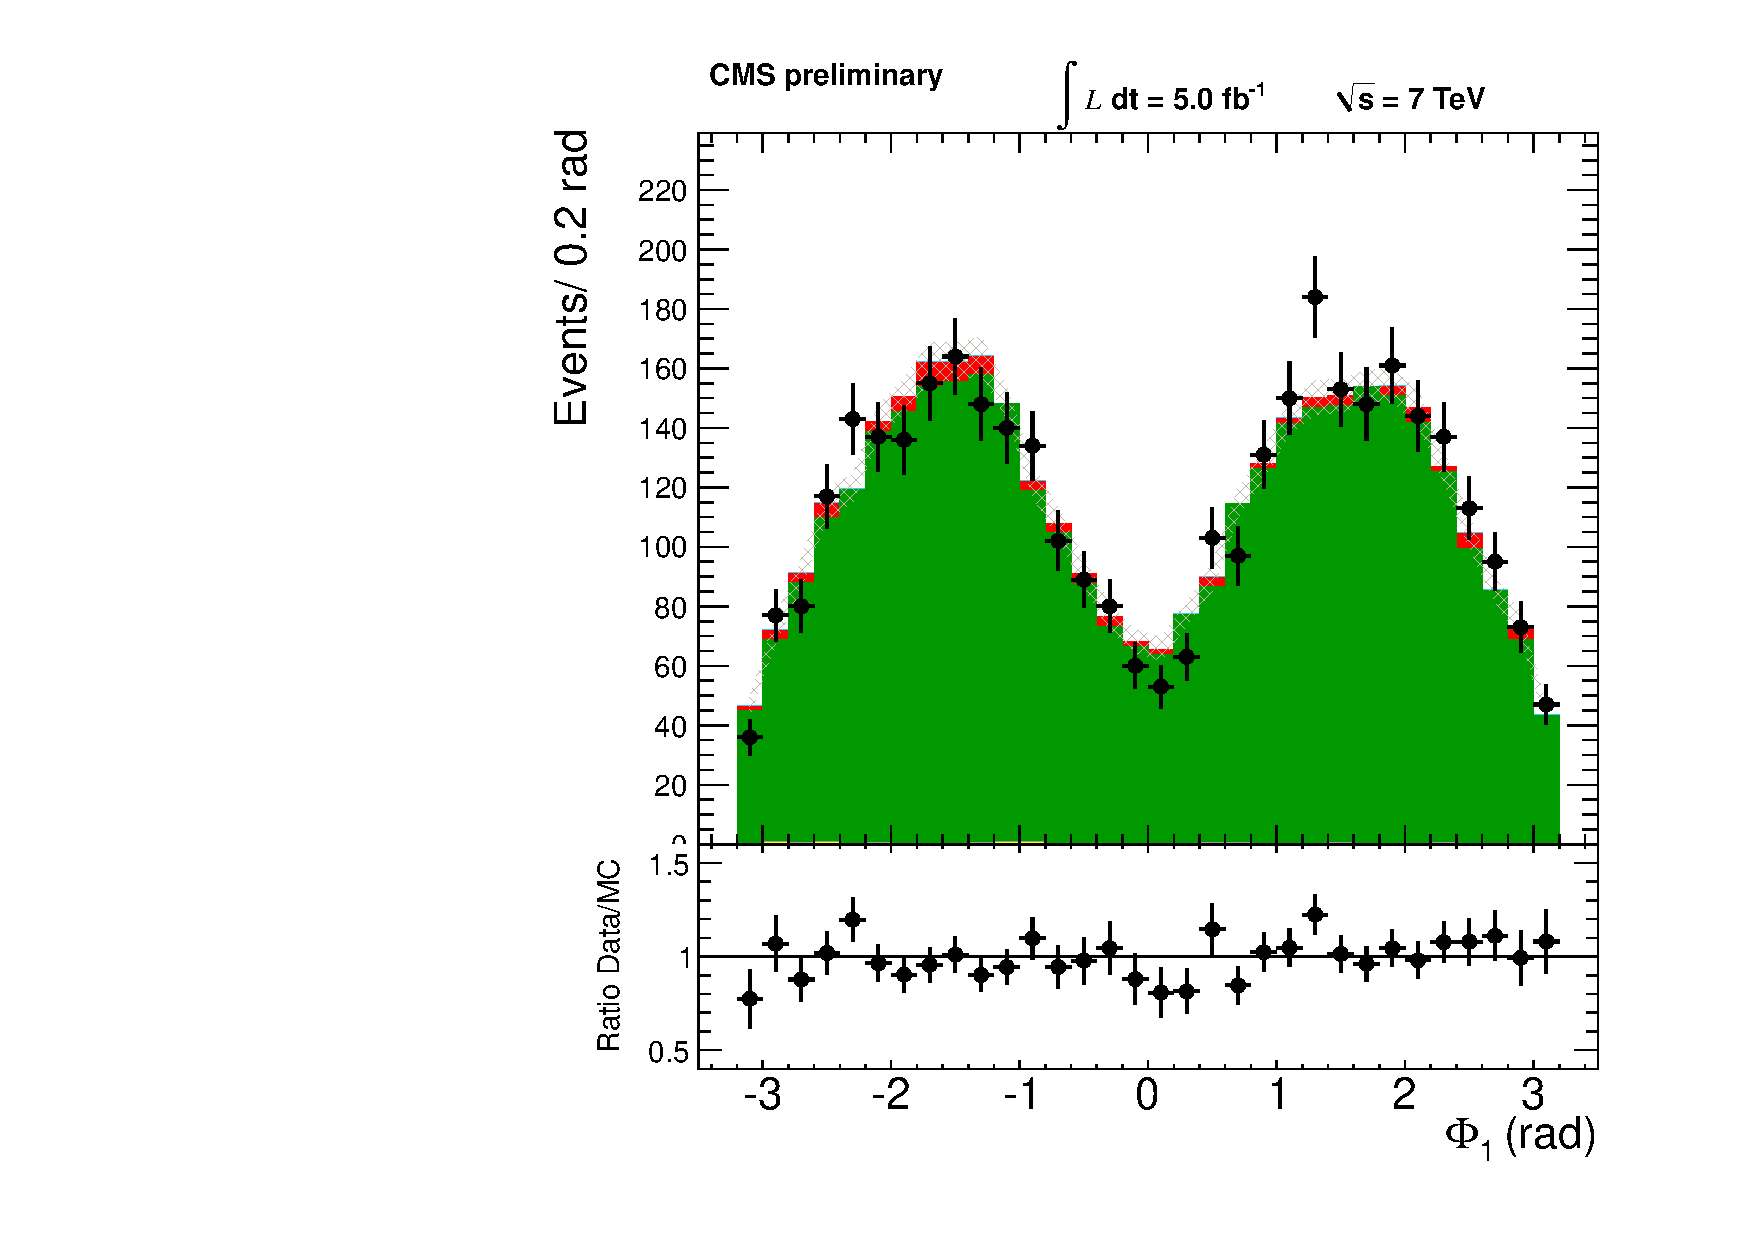
\includegraphics[width=0.49\textwidth]{figs/DataMC_ttbar/mu_phib.pdf}
    \caption{Comparison of the angular distributions for $\Phi$  (left)$\Phi_{1}$ (right) from data and 
      MC for the muon+jets selection.}
\label{fig:mu_ttbar_phi}}
\end{figure}

%%%%%%%%%%%%%%%%%%%%%%%%%%%%
\begin{figure}[h!t]
  {\centering
    \includegraphics[width=0.49\textwidth]{figs/DataMC_ttbar/mu_charge.pdf}
    \caption{Comparison of the charge of the muon from data and MC for the muon+jets selection.}
\label{fig:mu_ttbar_chg}}
\end{figure}

% rapidity and pt of the WW system

%%%%%%%%%%%%%%%%%%%%%%%%%%%%
\begin{figure}[h!t]
  {\centering
    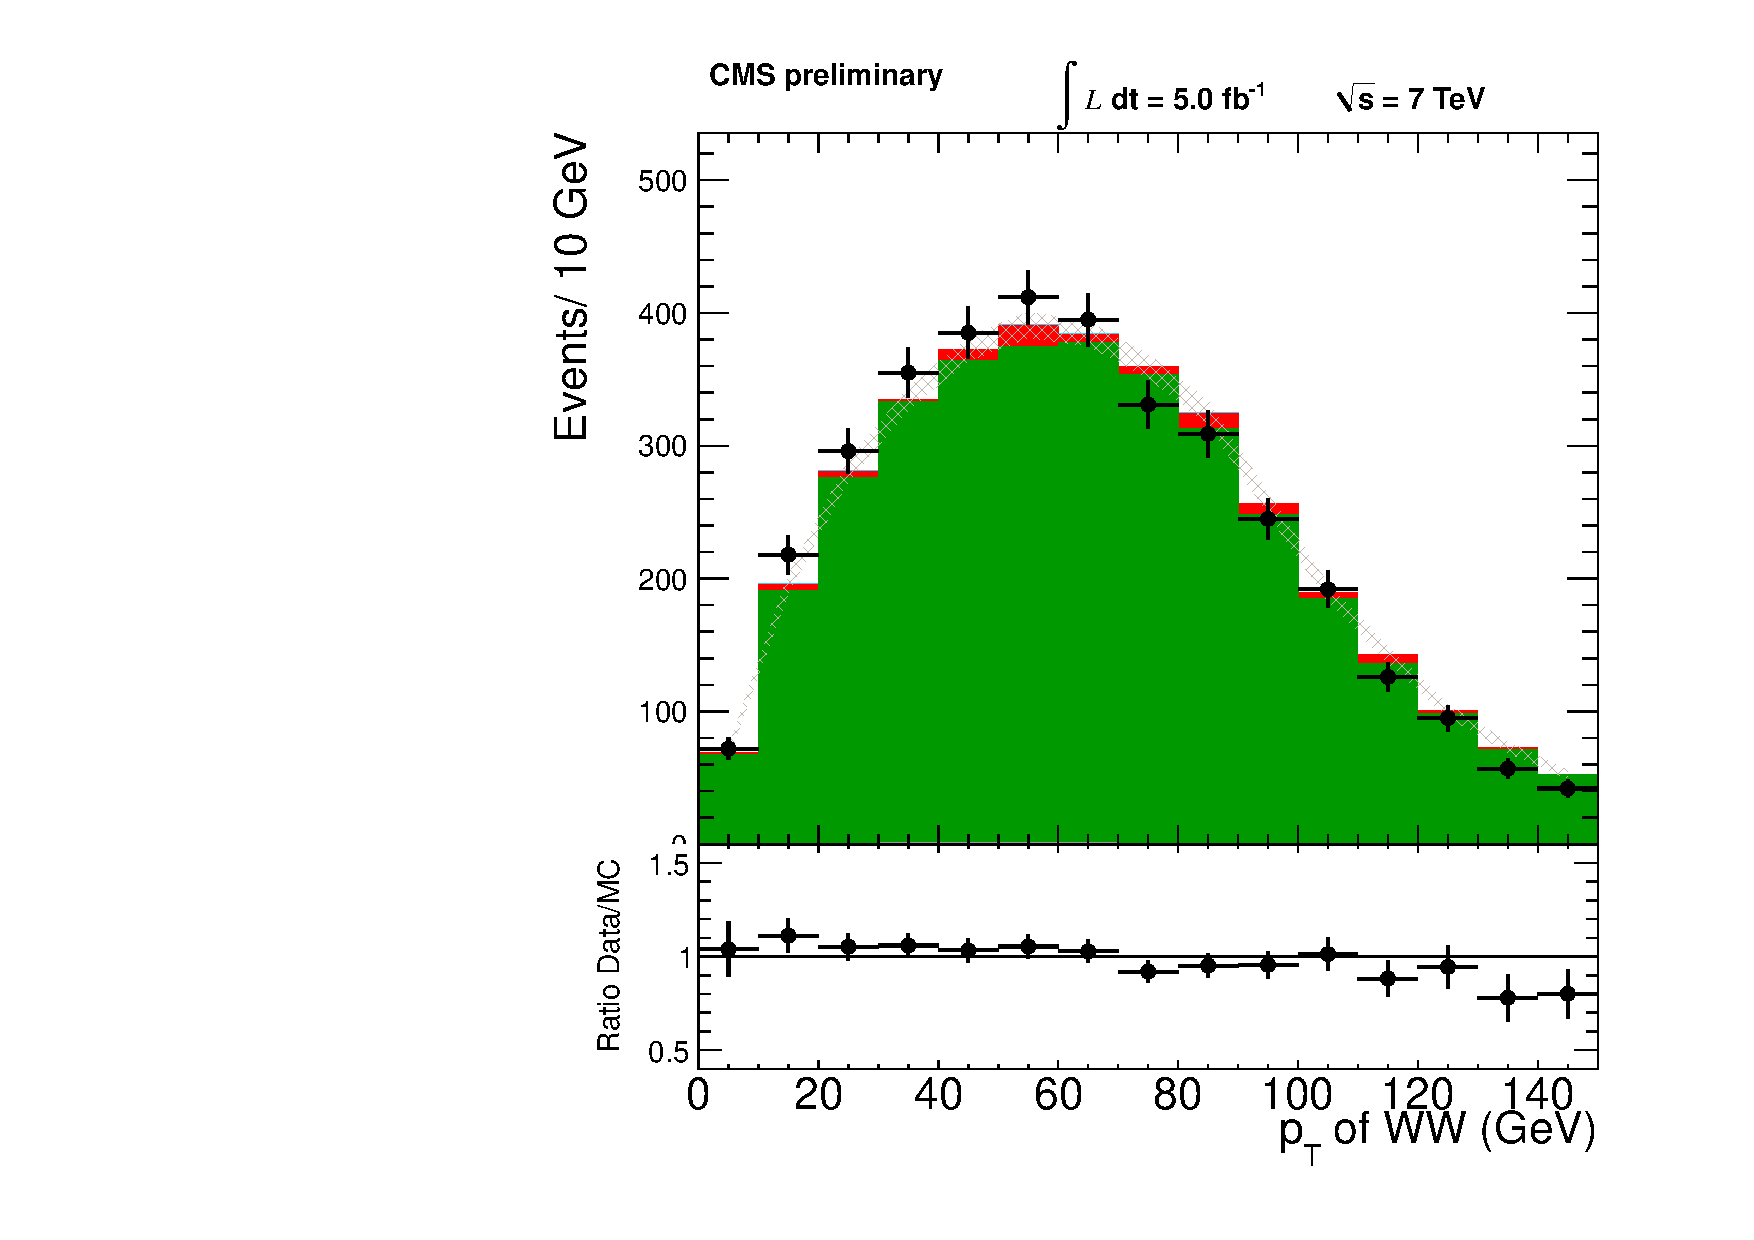
\includegraphics[width=0.49\textwidth]{figs/DataMC_ttbar/mu_ptlvjj.pdf}
    \includegraphics[width=0.49\textwidth]{figs/DataMC_ttbar/mu_etalvjj.pdf}
    \caption{Comparison of the $p_{T}$ (left) $\eta$ (right) of the WW system
      from data and MC for the muon+jets selection.}
\label{fig:mu_ttbar_ww}}
\end{figure}

%%%%%%%%%%%%%%%%%%%%%%%%%%%%%%%%%
%%%%%%%%%%%%%%%%%%%%%%%

% quark-gluon discriminants
%%%%%%%%%%%%%%%%%%%%%%%%%%%%
\begin{figure}[h!t]
  {\centering
    \includegraphics[width=0.49\textwidth]{figs/DataMC_ttbar/el_jetld_qgl.pdf}
    \includegraphics[width=0.49\textwidth]{figs/DataMC_ttbar/el_jetnt_qgl.pdf}
    \caption{Comparison of the Quark-gluon likelihood distributions for leading jet (left)
    second leading (right) from data and MC for the electron+jets selection.}
\label{fig:elec_ttbar_jet_qgl}}
\end{figure}
% angular variables
%%%%%%%%%%%%%%%%%%%%%%%%%%%%
%%%%%%%%%%%%%%%%%%%%%%%%%%%%
\begin{figure}[h!t]
  {\centering
    \includegraphics[width=0.49\textwidth]{figs/DataMC_ttbar/el_ha.pdf}
    \includegraphics[width=0.49\textwidth]{figs/DataMC_ttbar/el_hb.pdf}
    \caption{Comparison of the angular distributions for $\cos\theta_{1}$ (left)
   $\cos\theta_{2}$ (right) from data and MC for the electron+jets selection.}
\label{fig:elec_ttbar_theta}}
\end{figure}
%%%%%%%%%%%%%%%%%%%%%%%%%%%%
\begin{figure}[h!t]
  {\centering
     \includegraphics[width=0.49\textwidth]{figs/DataMC_ttbar/el_hs.pdf}
    \caption{Comparison of the angular distributions for $\cos\theta^{\ast}$ from data and MC 
   for the electron+jets selection.}
\label{fig:elec_ttbar_thetas}}
\end{figure}
%%%%%%%%%%%%%%%%%%%%%%%%%%%%
\begin{figure}[h!t]
  {\centering
    \includegraphics[width=0.49\textwidth]{figs/DataMC_ttbar/el_phi.pdf}
    \includegraphics[width=0.49\textwidth]{figs/DataMC_ttbar/el_phib.pdf}
    \caption{Comparison of the angular distributions for $\Phi$  (left)
    $\Phi_{1}$ (right) from data and MC for the 
    electron+jets selection.}
\label{fig:elec_ttbar_phi}}
\end{figure}

%%%%%%%%%%%%%%%%%%%%%%%%%%%%
\begin{figure}[h!t]
  {\centering
    \includegraphics[width=0.49\textwidth]{figs/DataMC_ttbar/el_charge.pdf}
    \caption{Comparison of the charge of the electron from data and MC for the electron+jets selection.}
\label{fig:elec_ttbar_chg}}
\end{figure}

% rapidity and pt of the WW system

%%%%%%%%%%%%%%%%%%%%%%%%%%%%
\begin{figure}[h!t]
  {\centering
    \includegraphics[width=0.49\textwidth]{figs/DataMC_ttbar/el_ptlvjj.pdf}
    \includegraphics[width=0.49\textwidth]{figs/DataMC_ttbar/el_etalvjj.pdf}
    \caption{Comparison of the $p_{T}$ (left) $\eta$ (right) of the WW system
      from data and MC for the electron+jets selection.}
\label{fig:elec_ttbar_ww}}
\end{figure}

%%%%%%%%%%%%%%%%%%%%%%%%%%%%
\clearpage

\section{Optimization of likelihoods}
\label{sec:mvaoptimization}

Using a complete set of mostly uncorrelated variables we optimize each
Higgs mass points separately to distinguish between the Higgs signal
and the dominant W+jets background.  To achieve a better S/B
separation we split the data into four categories -- electron 2-jets,
electron 3-jets, muon 2-jets, and muon 3-jets, and optimize each
category separately. We implemented a multi-variate analysis (MVA) and
used likelihood as the only classifier. The details of the likelihood
optimization are described in detail in the CMS analysis note
AN-2012/008.

We cut on the output of the classifier.  To deterine the optimal cut,
we step through the cut values and for each run the entire analysis
and limit setting machinery.  We then use the expected limit to derive
our choice of cut.  This correctly accounts for the signal and
background as well as the sytematics on each.  Examples of this
optimization are shown in Fig.~\ref{fig:optCut}.  The lower the
expected limit the better the cut is judged to be.

One discriminating variable was left out of the multi-variate analysis
so that a selection on this variable could be applied separately and
in parallel with the MVA output cut.  The quark-gluon likelihood
discriminant gives a measure of the likelihood of a jet originating
from a quark or gluon~\cite{qgAN}.  At leading order, the SM Higgs
signal consists of quark-originated jets while the background is an
admixture of both quark- and gluon-originated jets.

The details of the implementation of the quark-gluon likelihood discriminator
are covered in CMS AN-2011/110, Section 8.2. The cut value of the discriminator
was optimized in exactly the same way as the MVA likelihood discriminator,
excepting that the MVA selection was applied first when the scan over cut
values was performed.

\begin{figure}
\begin{center}
\includegraphics[width=0.3\textwidth]{figs/mu2jet180Optimize}
\includegraphics[width=0.3\textwidth]{figs/mu2jet350Optimize}
\includegraphics[width=0.3\textwidth]{figs/mu2jet500Optimize}
\end{center}
\caption{examples of cut optimization for three points all muon, 2 jet
samples with Higgs masses of 180 GeV (left), 350 GeV (center) and 500
GeV (right).}
\label{fig:optCut}
\end{figure}
%%%%%%%%%%%%%%%%%%%%%%%%%%%%%%%
%%%%%%%%%%%%%%%%%%%%%%%%%%%%%%%
%%%%%%%%%%%%%%%%%%%%%%%%%%%%%%%%%%%%%%%%%%%%%%%%%%%%%%%%%%%%%%%%%%%%
%%%%%%%%%%%%%%%%%%%%%%%%%%%%%%%%%%%%%%%%%%%%%%%%%%%%%%%%%%%%%%%%%%%%
%%%%%%%%%%%%%%%%%%%%%%%%%%%%%%%%%%%%%%%%%%%%%%%%%%%%%%%%%%%%%%%%%%%%
%%%%%%%%%%%%%%%%%%%%%%%%%%%%%%%%%%%%%%%%%%%%%%%%%%%%%%%%%%%%%%%%%%%%
%%%%%%%%%%%%%%%%%%%%%%%%%%%%%%%%%%%%%%%%%%%%%%%%%%%%%%%%%%%%%%%%%%%%
%%%%%%%%%%%%%%%%%%%%%%%%%%%%%%%%%%%%%%%%%%%%%%%%%%%%%%%%%%%%%%%%%%%%
%%%%%%%%%%%%%%%%%%%%%%%%%%%%%%%%%%%%%%%%%%%%%%%%%%%%%%%%%%%%%%%%%%%%
\section{Data driven QCD estimation}
\label{sec:qcd}
A background from QCD multijet events comes from 3- or 4-jet events
with one jet passing the lepton criteria as a 'fake'. However, it is
not practical to generate sufficient MC to create a statistically
significant sample that passes the selection criteria. Therefore we
rely on a data-driven approach in which the isolation-inverted samples
from data, which mirror the QCD background, are used instead.
Specifically, we perform a two-component simultaneous fit to data of
the MET distribution in order to obtain the fraction of QCD events in
the data; the two components are a data-based QCD sample and a
MC-based W+Jets sample.

The data sample is constrained to a specific trigger epoch from Run
2011A, comprising approximately 200~$\pbinv$, in which the isolation
requirement in the trigger was loose enough to allow for the inversion
and thereby provide sufficient statistics for the study. The QCD sample is
obtained by inverting the lepton isolation in this data sample to be
$>0.1$ (default selection uses Iso$_{mu}<0.1$ and Iso$_{el}<0.05$).
In order to increase statistics for the QCD sample we also relax the
MET cut from 30~GeV to 20~GeV and (for electrons) the ID requirement
to WP90-like.  The MC W+Jets and target data samples are obtained by
similarly relaxing the MET cut and ID requirements.

The fraction of QCD events in data is then obtained from a
simultaneous fit of the two components on the MET distribution
performed before the MVA cut, again to maintain sufficient statistics.
The W+jets normalization is left free to float, as well as the QCD;
the results are shown in Figure~\ref{fig:QCDTemplateFit_MET}.  We
subsequently adjust the fraction applicable to our analysis by
removing the portion of events for which 20$<$MET$<$30~GeV, and
estimate the fraction of QCD relative to the data as shown in
Table~\ref{tab:qcdfrac}.  A separate study verified
that the fraction of QCD was not sensitive to the MVA selection;
nevertheless, to account for discrepancies in template modeling
(e.g. using W+jets MC as a proxy for all non-QCD processes) and the
fact that this fraction is estimated prior to the MVA cut, a very
large uncertainty is conservatively assumed. The final fraction of QCD
events in data is fed to the $m_{jj}$ fit for determination of the QCD
normalization, and the four-body shape of the QCD distribution is fed
to the final four-body total background determination in preparation
for the limit setting procedure.

Note that the W transverse mass distributions from the data and MC are
statistically consistent, as shown in
Figure~\ref{fig:QCDCutLoosening_MET} for muons; for electrons there's
an insufficient number of MC events to make the comparison.  The MET
for QCD processes is also 'fake'; i.e., it originates from badly
measured jets, and therefore has an exponentially falling spectrum.
By contrast, all other backgrounds exhibit a wide peak at $\sim
35$~GeV from a real neutrino (with the exception of Z+Jets, where the
MET is the result of a poorly measured lepton).

%%  $el_{2J}$ $frac_{QCD}=0.0617\pm 0.00384$,
%%  $el_{3J}$ $frac_{QCD}=0.0213\pm 0.00678$.
%%
%% $\mu_{2J}$ $frac_{QCD}=0.001625\pm 0.004214$,
%% $\mu_{3J}$ $frac_{QCD}=0.0\pm 0.0040797$,


\begin{table}[bthp]
\begin{center}
  \begin{tabular}{l c c}
    \hline  \hline
     & 2 jets & 3 jets \\
    \hline  
    electron  &	6.2 $\pm$ 0.4\% & 2.1 $\pm$ 0.7\% \\
    muon      &	0.2 $\pm$ 0.4\% & 0.0 $\pm$ 0.4\% \\
    \hline  \hline
  \end{tabular}
\end{center}
\caption{\label{tab:qcdfrac} Estimates of the percentage of QCD in data
for the muon and electron datasets after selection, separated into 2- and
3-jet bins.}
\end{table}

\subsection{QCD Uncertainties}
\label{sec:qcd_Uncertainty}

When performing the $m_{jj}$ fit  the QCD yield 
is Gaussian-constrained with a mean given by the value shown in
Table~\ref{tab:qcdfrac}.
In the case of electrons, the error on the QCD fraction
is small and we (conservatively) estimate
the uncertainty to be one half of the expected value. For muons the 
uncertainty is the error on the relative fraction (i.e.,
0.4\% for both 2- and 3-jet bins).
When fitting the sum of electron and muon data, the uncertainties
are combined using the standard error propagation machinery.

\subsection{Cross-Checks}
In order to ensure that our inverted selection provides a consistent representation of
QCD events, we perform the following cross-checks:
\begin{itemize}
\item Fit the QCD with a Raileigh Function: $xe^{-x^2/2(\sigma_0+\sigma_1x)^2}$,
used during the inclusive cross section measurements~\cite{WZCMS:2010}. 
As can be seen from Fig.~\ref{fig:QCDMETRaileighFit},
the function accurately fits the overall shape as well as the parameter
corresponding to the intrinsic MET resolution ($\sigma_0\simeq 10$~GeV).
\item Compare the W transverse mass shapes for the data sidebands with MET$>20$~GeV vs 
MET$>30$~GeV (Fig.~\ref{fig:QCDMETCutsWmTShape}). Naturally, events with MET$>30$~GeV do not have the
same exponential falloff, since they contain a higher percentage of W's.
\item Examine the impact of setting Iso$>0.1$, rather than Iso$>0.2$.
We compare the MET (Fig.~\ref{fig:QCDISOCutsMETShape}) and W transverse mass
(Fig.~\ref{fig:QCDISOCutsWmTShape}) distributions, and conclude that there is no statistically
significant discrepancy introduced by the looser isolation requirement.
\end{itemize}


%%%%%%%%%%%%%%%%%%%%%%%%%%%%
%%%%%%%
\begin{figure}[h!] {\centering
\unitlength=0.33\linewidth
\includegraphics[width=0.48\textwidth]{figs/qcd/QCDDataVSMC_Muons2J_MET.pdf}
\caption{ Comparison of the MET shapes for MC vs data-driven muon QCD events in the 2-jet bin. The two are statistically consistent.} 
\label{fig:QCDCutLoosening_MET}
}
\end{figure}
%%%%%%%
%%%%%%%
\begin{figure}[h!] {\centering
\unitlength=0.33\linewidth
\includegraphics[width=0.48\textwidth]{figs/qcd/TemplateFit_MET_mu2j.pdf}
\put(-0.80,0.0){(a)} 
\unitlength=0.33\linewidth
\includegraphics[width=0.48\textwidth]{figs/qcd/TemplateFit_MET_mu3j.pdf}
\put(-0.80,0.0){(b)} \\
\unitlength=0.33\linewidth
\includegraphics[width=0.48\textwidth]{figs/qcd/TemplateFit_MET_el2j.pdf}
\put(-0.80,0.0){(c)} 
\unitlength=0.33\linewidth
\includegraphics[width=0.48\textwidth]{figs/qcd/TemplateFit_MET_el3j.pdf}
\put(-0.80,0.0){(d)} 
\caption{MET distributions fit to the QCD and W$jj$ templates for: (a) muons - 2-jet bin, (b) muons - 3-jet bin, (c) electrons - 2-jet bin, (d) electrons - 3-jet bin.} 
\label{fig:QCDTemplateFit_MET}
}
\end{figure}
%%%%%%%
%%%%%%%
\begin{figure}[h!] {\centering
\unitlength=0.33\linewidth
\includegraphics[width=0.48\textwidth]{figs/qcd/RaileighFitQCD_mu2j.pdf}
\put(-0.80,0.0){(a)} 
\unitlength=0.33\linewidth
\includegraphics[width=0.48\textwidth]{figs/qcd/RaileighFitQCD_mu3j.pdf}
\put(-0.80,0.0){(b)} \\
\unitlength=0.33\linewidth
\includegraphics[width=0.48\textwidth]{figs/qcd/RaileighFitQCD_el2j.pdf}
\put(-0.80,0.0){(c)} 
\unitlength=0.33\linewidth
\includegraphics[width=0.48\textwidth]{figs/qcd/RaileighFitQCD_el3j.pdf}
\put(-0.80,0.0){(d)} 
\caption{QCD MET distributions fitted with a Raileigh Function for: (a) muons - 2-jet bin, (b) muons - 3-jet bin, (c) electrons - 2-jet bin, (d) electrons - 3-jet bin.} 
\label{fig:QCDMETRaileighFit}
}
\end{figure}
%%%%%%%
%%%%%%%
\begin{figure}[h!] {\centering
\unitlength=0.33\linewidth
\includegraphics[width=0.48\textwidth]{figs/qcd/METShapeComp_mu2j.pdf}
\put(-0.80,0.0){(a)} 
\unitlength=0.33\linewidth
\includegraphics[width=0.48\textwidth]{figs/qcd/METShapeComp_mu3j.pdf}
\put(-0.80,0.0){(b)} \\
\unitlength=0.33\linewidth
\includegraphics[width=0.48\textwidth]{figs/qcd/METShapeComp_el2j.pdf}
\put(-0.80,0.0){(c)} 
\unitlength=0.33\linewidth
\includegraphics[width=0.48\textwidth]{figs/qcd/METShapeComp_el3j.pdf}
\put(-0.80,0.0){(d)} 
\caption{ QCD W transverse mass shapes with MET$>20$~GeV vs MET$>30$~GeV for: (a) muons - 2-jet bin, (b) muons - 3-jet bin, (c) electrons - 2-jet bin, (d) electrons - 3-jet bin.} 
\label{fig:QCDMETCutsWmTShape}
}
\end{figure}
%%%%%%%
%%%%%%%
\begin{figure}[h!] {\centering
\unitlength=0.33\linewidth
\includegraphics[width=0.48\textwidth]{figs/qcd/ISOShapeComp_MET_mu2j_g01vg02.pdf}
\put(-0.80,0.0){(a)} 
\unitlength=0.33\linewidth
\includegraphics[width=0.48\textwidth]{figs/qcd/ISOShapeComp_MET_mu3j_g01vg02.pdf}
\put(-0.80,0.0){(b)} \\
\unitlength=0.33\linewidth
\includegraphics[width=0.48\textwidth]{figs/qcd/ISOShapeComp_MET_el2j_g01vg02.pdf}
\put(-0.80,0.0){(c)} 
\unitlength=0.33\linewidth
\includegraphics[width=0.48\textwidth]{figs/qcd/ISOShapeComp_MET_el3j_g01vg02.pdf}
\put(-0.80,0.0){(d)} 
\caption{ QCD MET shapes with Iso$>0.1$ vs Iso$>0.2$ for: (a) muons - 2-jet bin, (b) muons - 3-jet bin, (c) electrons - 2-jet bin, (d) electrons - 3-jet bin.} 
\label{fig:QCDISOCutsMETShape}
}
\end{figure}
%%%%%%%
%%%%%%%
\begin{figure}[h!] {\centering
\unitlength=0.33\linewidth
\includegraphics[width=0.48\textwidth]{figs/qcd/ISOShapeComp_WmT_mu2j_g01vg02.pdf}
\put(-0.80,0.0){(a)} 
\unitlength=0.33\linewidth
\includegraphics[width=0.48\textwidth]{figs/qcd/ISOShapeComp_WmT_mu3j_g01vg02.pdf}
\put(-0.80,0.0){(b)} \\
\unitlength=0.33\linewidth
\includegraphics[width=0.48\textwidth]{figs/qcd/ISOShapeComp_WmT_el2j_g01vg02.pdf}
\put(-0.80,0.0){(c)} 
\unitlength=0.33\linewidth
\includegraphics[width=0.48\textwidth]{figs/qcd/ISOShapeComp_WmT_el3j_g01vg02.pdf}
\put(-0.80,0.0){(d)} 
\caption{ QCD W transverse mass shapes with Iso$>0.1$ vs Iso$>0.2$ for: (a) muons - 2-jet bin, (b) muons - 3-jet bin, (c) electrons - 2-jet bin, (d) electrons - 3-jet bin.} 
\label{fig:QCDISOCutsWmTShape}
}
\end{figure}
%%%%%%%
%%%%%%%%%%%%%%%%%%%%%%%%%%%%%%%%%%%%%%%%%%%%%%%%%%%%%%%%%%%%%%%%%%%%
%%%%%%%%%%%%%%%%%%%%%%%%%%%%%%%%%%%%%%%%%%%%%%%%%%%%%%%%%%%%%%%%%%%%
%%%%%%%%%%%%%%%%%%%%%%%%%%%%%%%%%%%%%%%%%%%%%%%%%%%%%%%%%%%%%%%%%%%%
\clearpage
%%%%%%%%%%%%%%%%%%%%%%%%%%%%%%%%%%%%%%%%%%%%%%%%%%
%%%%%%%%%%%%%%%%%%%%%%%%%%%%%%%%%%%%%%%%%%%%%%%%%%
\section{Modeling of W+jets background shape in \texorpdfstring{$m_{jj}$}{dijet invariant mass} }
\label{sec:wjetsShape}
%%%%%%%%%%%%%
%\begin{figure}
%\begin{center}
%\includegraphics[width=\textwidth,trim=0 150 0 150,clip]{figs/mjjdfd2body}
%\end{center} 
%\caption{\label{fig:mjj2body}A depiction of the inputs and work flow of the W+jets template and the final fit.}
%\end{figure} 
%%%%%%%%%%%%%
%In order to get a good description of the W+jets shape in data, the 
%simulation needs to describe well both the matrix elements for the 
%hard processes, and 
%the subsequent development of the hard partons into jets of hadrons. 
%However, no factorization theorem exists to rigorously separate
%these two components. 
%A given (n + 1)-jet event can be obtained in two ways: from the 
%collinear/soft-radiation
%evolution of an appropriate (n + 1)-parton final state, or from 
%an n-parton configuration
%where hard, large-angle emission during its evolution leads to the extra jet. 
%A factorization scheme defines, on an event-by-event basis, which of 
%the two paths should be followed.
%The two relevant parameters defining such 
%a scheme are: the factorization/renormalization scale $q^2$ and the 
%matrix element - parton shower matching threshold.
%Optimized values of these parameters should give the best possible 
%approximation 
%to the W+jets kinematics for a given fixed-order calculation.
%We know that  the physics has to be independent of the relative contributions  
%of the two components.
%Therefore, it is important to assess the systematic uncertainty 
%in the W+jets shape due to the choice of these parameters.  


%%%%%%%%%%%%%%%%
%\begin{figure}
%\begin{center}
%\includegraphics[width=0.75\textwidth]{figs/Wjets_shapes}
%\end{center}
%\caption{\label{fig:wjetshapes}The $m_{jj}$ distribution in W+jets events for various
%MC samples.}
%\end{figure}
%%%%%%%%%%%%%%%%
%
%To determine the expected number of W+jets events in the signal region,
%it is necessary to know its shape in the $m_{jj}$ variable.
%
%Because of inadequate statistics in the W+jets MC and the overal poor
%agreement between W+jets MC and many data distibutions, we employ an
%emperical description of the W+jets shape.  This description is a
%kinematic turn on and a power law tail:
%\begin{equation}
%  \mathcal{F}_{W+\text{jets}} = \text{erf}(m_{jj}; m_0, \sigma)\times\left[(m_{jj})^{-\alpha-\beta\ln(m_{jj}/\sqrt{s})}\right]\,,
%\end{equation}
%where $m_0$ is the value of the turn on and $\sigma$ is the width of
%this turn on.  The parameters $m_0$, $\sigma$, $\alpha$ and $\beta$
%are determined in the fit to the data after the MVA cut.
%
%This nominal fit shape is not particularly well suited for all of the
%mass points.  In the 2-jet channels for masses from 200 GeV and below
%we use the following fit fucntion
%\begin{equation}
%  \mathcal{F}_{W+\text{jets low mass, 2 jets}} = \text{erf}(m_{jj}; m_0, \sigma)\times(m_{jj})^{-\alpha}\times\exp(m_{jj}\tau)\,,
%\end{equation}
%where the parameters $m_0$, $\sigma$, $\alpha$ and $\tau$ are
%determined in the fit.  In the 3-jet channels we use the
%parameterization
%\begin{equation}
%  \mathcal{F}_{W+\text{jets low mass, 3 jets}} = (m_{jj})^{-\alpha-\beta\ln(m_{jj}/\sqrt(s))}\times\exp(m_{jj}\tau)
%\end{equation}
%for masses from 300 GeV and below.  The parameter $\beta$ is fixed to
%zero for the mass points from 200 GeV and below.

The fit of the $m_{jj}$ spectrum is described in Section 10 of CMS AN 2011/110.  The line shapes used
are detailed as well as the parameters which float.
The projections of the fits to data for each of the mass, flavor and jet number bins are in
Figs.~\ref{fig:mjj_mH170}--\ref{fig:mjj_mH600}.

%The CMS MadGraph W+jets production uses MLM matching \cite{Hoche:2006ph} with $k_T$ jets.
%The default matching threshold is 10~GeV (i.e.,
%if the parton $p_{T}$  is greater than 10~GeV, then it is assumed to 
%have originated from the hard scattering process and contributes to the matrix element 
%calculation; if the parton $p_{T}$ is less than 10~GeV then it is assumed 
%to come from the parton shower). 
%The factorization/renormalization scale 
%$q^2$ corresponds to the ``transverse mass'' of the W boson: 
%$\sqrt{M_W^2 + p_{T, W}^2}$.  


%To perform studies of the systematic uncertainty due to the choice of
%the $q^2$ and matching scales, alternative MadGraph W+jets samples are
%produced in which the corresponding scales are changed by a factor of 2.
%Thus, we have ``matching-up'', ``matching-down'', ``scale-up'', and
%``scale-down'' samples, each yielding an $m_{jj}$ distribution, or
%template.  Our use of these templates is shown schematically in
%Fig.~\ref{fig:mjj2body} and described below.
%Figure~\ref{fig:wjetshapes} shows the input MC $m_{jj}$ templates that
%are used.

%We can use our samples to find an optimum MC template $\mathcal{F}_{W+\text{jets}}$,
%\[
%\mathcal{F}_{W+\text{jets}} = \sum_\alpha f_\alpha \mathcal{G}_\alpha\, + (1-\sum_\alpha f_\alpha)\times\mathcal{G}_\text{nominal},
%\]
%where $\alpha \in
%\{\text{matchingUp,matchingDown,scaleUp,scaleDown}\}$,
%$\mathcal{G}_\text{nominal}$ is the template from the default MadGraph
%generation and $\mathcal{G}_\alpha$ is the template from the specified
%sample.  We define a 2D coordinate system in scale and matching.  The
%origin corresponds to the default MadGraph sample.  To move in the
%positive scaleUp direction, one sets $f_\text{scaleDown}=0$ and
%increases $f_\text{scaleUp}$. To move in the negative scaleUp
%direction, one sets $f_\text{scaleUp}=0$ and increases
%$f_\text{scaleDown}$.  The same is true for the matching samples.  We
%let these parameters float in the $m_{jj}$ fit.

%%%%%%%%%%%%%%%%%%%%%%%%%%%%%%%%%%%%%%%%%%%%%%%%%%
%%%%%%%%%%%%%%%%%%%%%%%%%%%%%%%%%%%%%%%%%%%%%%%%%%
%\clearpage
%%%%%%%%%%%%%%%%%%%%%%%%%%%%%%%%%%%%%%%%
%%%%%%%%%%%%%%%%%%%%%%%%%%%%%%%%%%%%%%%%
\section{Jet Energy Scale from the hadronic W in top quark events}
\label{sec:topw}
We reconstruct the hadronic W candidate from an almost pure top data control sample. 
The semileptonic top
events are selected by requiring exactly four jets in the event, out of
which two are b-tagged and the other two are anti-btagged. The
hadronic W candidates are formed from two anti-btagged jets. 
The invariant mass of the hadronic W candidates in the muon,
electron, and combined channels are shown in 
Figs.~\ref{fig:topw:mu},~\ref{fig:topw:el}, and 
\ref{fig:topw:muel}, respectively.  When we propagate the difference in the JES to our
templates and signal shapes they make a negligible difference.
%%%%%%%%%%%%%%%%%%%%%
\begin{figure}[htb] 
  {\centering
    \includegraphics[width=0.325\textwidth]{figs/topwjes/top_overlap_mu.pdf}
    \includegraphics[width=0.325\textwidth]{figs/topwjes/top_data_fit_mu.pdf}
    \includegraphics[width=0.325\textwidth]{figs/topwjes/top_mc_fit_mu.pdf}
    \caption{The invariant mass distribution of the hadronic 
      W candidates in the muon semileptonic top sample. 
      The left plot shows good agreement between the data and MC. 
      We fit the distribution with a Gaussian and extract the peak
      location for the data (middle) and MC (right).}
    \label{fig:topw:mu}}
\end{figure}
%%%%%%%%%%%%%%
\begin{figure}[htb] 
  {\centering
    \includegraphics[width=0.325\textwidth]{figs/topwjes/top_overlap_el.pdf}
    \includegraphics[width=0.325\textwidth]{figs/topwjes/top_data_fit_el.pdf}
    \includegraphics[width=0.325\textwidth]{figs/topwjes/top_mc_fit_el.pdf}
    \caption{The invariant mass distribution of the hadronic 
      W candidates in the electron semileptonic top sample. 
      The left plot shows good agreement between the data and MC. 
      We fit the distribution with a Gaussian and extract the peak
      location for the data (middle) and MC (right).}
    \label{fig:topw:el}}
\end{figure}
%%%%%%%%%%%%%
\begin{figure}[htb] 
  {\centering
    \includegraphics[width=0.325\textwidth]{figs/topwjes/top_overlap_muel.pdf}
    \includegraphics[width=0.325\textwidth]{figs/topwjes/top_data_fit_muel.pdf}
    \includegraphics[width=0.325\textwidth]{figs/topwjes/top_mc_fit_muel.pdf}
    \caption{The invariant mass distribution of the hadronic 
      W candidates in the semileptonic top sample (electron and 
      muon combined). 
      The left plot shows good agreement between the data and MC. 
      We fit the distribution with a Gaussian and extract the peak
      location for the data (middle) and MC (right).}
    \label{fig:topw:muel}}
\end{figure}
%%%%%%%%%%%%%%%%%%%%%%%%%%%%%%%%%%%%%%%%%%%%%%%%%%%%%%%%%%%%%%%%%%%%%%%%%%%

\section{Kinematic fit}
\label{sec:kineFit}

In order to improve the mass resolution in the four body mass measurement, 
a two constraint (2C) fit with one unknown, 
the neutrino z momentum component, was made. 
The constraints were that the lepton-neutrino pair and the di-jet system
both separately form an invariant mass equal to the W mass to within its
known width.
The infrastructure of the fit uses standard CMS kinematic tools. % \cite{rf:CMSKineFit}.
The four particles are part of the fit, 
with a covariance matrix supplied in the fit for the jets and the lepton.
%FIXME where does this covariance matrix come from? 
The neutrino has small errors assigned, by hand,  
to the unknown z component of the momentum and the x and y transverse components.
The starting value input to the fit for the x and y components of the neutrino 
is the measured missing transverse energy along the x and y axes, 
while the $z$ component is chosen as the solution with the smallest absolute value 
(or the one that produces the neutrino closest to the lepton).
In case no real solution is found, 
the real part of the solution is used.
% No additional constraints on the missing energy.
%% One unique part of the fit was to impose the coupling of the jet energy variation 
%% into the global variable of the missing transverse energy.
%% A constraint that the x and y components of the four particles in the final state be zero was imposed.
%% That means that variations in the jet energies propagate into correlated variations 
%% of the neutrino x and y momentum components.
%The mass spectrum for a Higgs boson with 200 GeV mass is shown in Fig. xxx 
%before and after the kinematic fit. 

The improved resolution in the four body mass is a crucial ingredient in the Higgs search. 
Without the improved resolution, 
the rise and fall of the low mass spectrum of electroweak WW continuum production 
is not well resolved from a resonant Higgs mass spectrum 
were it to occur near the WW threshold in mass.
The kinematic fit also improves our ability to model the dominant
W+Jets background and reduce its shape uncertainty, which is one of
our dominant systematic uncertainties. Since the limit setter uses the
four-body shapes to distinguish signal from background, the kinematic
fit has a direct impact on the final limit.

Figure~\ref{fig:fitKFExample} shows the effect of the kinematic fit 
on the four-body mass distribution for the signal at the four lowest
mass points, as well as for WW and W+Jets.
The distributions obtained before and after the kinematic fit are reported.
The effect of the kinematic fit becomes less pronounced for increased signal mass.
%
\begin{figure}[htb]
    \subfigure[Higgs M=170~GeV]{
      \includegraphics[width=0.42\textwidth]{figs/kfcompare-Hww170.pdf}
    }
    \subfigure[Higgs M=180~GeV]{
      \includegraphics[width=0.42\textwidth]{figs/kfcompare-Hww180.pdf}
    }
    \\
    \subfigure[Higgs M=190~GeV]{
      \includegraphics[width=0.42\textwidth]{figs/kfcompare-Hww190.pdf}
    }
    \subfigure[Higgs M=200~GeV]{
      \includegraphics[width=0.42\textwidth]{figs/kfcompare-Hww200.pdf}
    }
    \\
    \subfigure[WW]{
      \includegraphics[width=0.42\textwidth]{figs/kfcompare-WW_low.pdf}
    }
    \subfigure[W+Jets]{
      \includegraphics[width=0.42\textwidth]{figs/kfcompare-Wjet_low.pdf}
    }
    \caption{The four-body mass distributions obtained before and
             after the kinematic fit are reported for the four lowest
             Higgs mass hypotheses as well as for WW and W+Jets
             backgrounds. The mass range is constrained to that used
             for subsequent template modeling and limit setting.}
    \label{fig:fitKFExample}
\end{figure}

\clearpage
%%%%%%%%%%%%%%%%%%%%%%%%%%%%%%%%%%%%%%%%%%%%%%%%%%
%%%%%%%%%%%%%%%%%%%%%%%%%%%%%%%%%%%%%%%%%%%%%%%%%%
%%%%%%%%%%%%%%%%%%%%%%%%%%%%%%%%%%%%%%%%%%%%%%%%%%
%%%%%%%%%%%%%%%%%%%%%%%%%%%%%%%%%%%%%%%%%%%%%%%%%%
\section{Extraction of W+jets background shape in \texorpdfstring{$m_{WW}$}{diboson invariant mass} from data sidebands}
\label{sec:alphaExtraction}
The four-body mass shape of the W+jets background in the signal region
is estimated in a data driven way from sidebands in the $m_{jj}$
region.

For each of the 48 working points of the MVA optimization, three
regions in $m_{jj}$ are looked at:
\begin{itemize}
\item lower sideband region (SBL):  $m_{jj} \in$ [55,65]~GeV
\item signal region: $m_{jj} \in $ [65,95]~GeV
\item upper sideband region (SBH): $m_{jj} \in$ [95,115] for $M_H<$250~GeV, [95,200]~GeV  for $M_H\ge$250~GeV, 
\end{itemize}

In the Monte Carlo, the $m_{\ell\nu jj}$ shapes in the upper and lower
sidebands are compared to the one in the signal region, to find the
best mixture of the first two that reproduce the latter.  Therefore an
$\alpha$ parameter is searched for, such that:
\begin{equation}
m_{WW_i}^{j} = (1-\alpha^j) \cdot m_{SBH_i}^j + \alpha^j \cdot  m_{SBL_i}^j~,
\label{EqnAlpha}
\end{equation}
where the index $j$ refers to each of the 48 mass spectra and $i$ to
the bins in the dijet mass.  In this way, the technique is largely
data driven but the precise extrapolation depends on the Monte Carlo
model. The value for the best alpha in $W+$jets MC and the
$\chi^2/$NDF scan of the shapes are shown in
Figs.~\ref{fig:mcalphacheck_2j350mu} as an example for the SM Higgs
mass of 350~GeV for the 2-jet $W\to\mu\nu$ category.

%
\begin{figure}[!t]
  \centering
  \includegraphics[width=0.49\textwidth]{figs/2j350mu-Alpha-mcget-MVAgt_60_Range_12_300-780_SB_55-65_95-200.pdf}
  \includegraphics[width=0.49\textwidth]{figs/2j350mu-Alpha-mcsca-MVAgt_60_Range_12_300-780_SB_55-65_95-200.pdf}
  \caption{\label{fig:mcalphacheck_2j350mu}The optimal alpha value
    from $W+$jets MC for the SM Higgs mass of 350~GeV for the 2-jet
    $W\to\mu\nu$ category.}
\end{figure}
%

%%%%%%%%%%%%%%%%%%%%%%%%%%%%%%%%%%%%%%%%%%%%%%%%%%%%%%%%%%%%%%%%%%%%%%%%%%%%%%
The distributions of the $m_{\ell\nu jj}$ shape in data are shown in
Figs.~\ref{fig:mlnujj_WpJShape_mH170}--\ref{fig:mlnujj_WpJShape_mH600}
for various Higgs mass points, lepton flavor and jet count.  Because
these shapes in general do not have copious statistics in them we fit
the shape using a binned likelihood method to an exponential shape.
As can be seen in the figures the low mass 2-jet electron shapes
deduced from the sidebands show a ``turn on'' kind of behavior.  When
we look at the MC in the signal region we don't observe this turn on
behavior except in the 190 GeV case.  In that case we put the turn on
behavior into the fitting model using a error function shape, where
the width of the turn on is fixed to 15\,GeV.  In the other cases we
simply exclude the first point from the sideband fit and use the
exponential extrapolation to go from 180 GeV to 170 GeV.  This
exponential shape is used at the template for the W+jets background of
the $m_{\ell\nu jj}$.  The uncertainty in the decay constant for the
exponential shape utilized as a systematic uncertainty in the limit
setting.
%%%%%%%%%%%%%%%%%%%%
%%%%%%%%%%%%%%%%%%%%
%%%%%%%%%%%%%%%%%%%%
\begin{figure}[h!t]
  {\centering
\subfigure[]{
    \includegraphics[width=0.48\textwidth]{figs/H170_Mlvjj_Muon_2jets_WpJShape}
}
\subfigure[]{
    \includegraphics[width=0.48\textwidth]{figs/H170_Mlvjj_Muon_3jets_WpJShape}
}
\vspace*{1mm} \\
\subfigure[]{
    \includegraphics[width=0.48\textwidth]{figs/H170_Mlvjj_Electron_2jets_WpJShape}
}
\subfigure[]{
    \includegraphics[width=0.48\textwidth]{figs/H170_Mlvjj_Electron_3jets_WpJShape}
}
\caption{$M_H = 170$~GeV point. The distribution of the $m_{\ell\nu jj}$ shape in data and its smooth parametrization. 
The four plots correspond to muon 2-jets, muon 3-jets, electron 2-jets, 
and electron 3-jets event categories, respectively. }
\label{fig:mlnujj_WpJShape_mH170}}
\end{figure}
%%%%%%%%%%%%%%%%%%%%
%%%%%%%%%%%%%%%%%%%%
%%%%%%%%%%%%%%%%%%%%
\begin{figure}[h!t]
  {\centering
\subfigure[]{
    \includegraphics[width=0.48\textwidth]{figs/H180_Mlvjj_Muon_2jets_WpJShape}
}
\subfigure[]{
    \includegraphics[width=0.48\textwidth]{figs/H180_Mlvjj_Muon_3jets_WpJShape}
}
\vspace*{1mm} \\
\subfigure[]{
    \includegraphics[width=0.48\textwidth]{figs/H180_Mlvjj_Electron_2jets_WpJShape}
}
\subfigure[]{
    \includegraphics[width=0.48\textwidth]{figs/H180_Mlvjj_Electron_3jets_WpJShape}
}
\caption{$M_H = 180$~GeV point. The distribution of the $m_{\ell\nu jj}$ shape in data and its smooth parametrization. 
The four plots correspond to muon 2-jets, muon 3-jets, electron 2-jets, 
and electron 3-jets event categories, respectively. }
\label{fig:mlnujj_WpJShape_mH180}
}
\end{figure}
%%%%%%%%%%%%%%%%%%%%
%%%%%%%%%%%%%%%%%%%%
%%%%%%%%%%%%%%%%%%%%
\begin{figure}[h!t]
  {\centering
\subfigure[]{
    \includegraphics[width=0.48\textwidth]{figs/H190_Mlvjj_Muon_2jets_WpJShape}
}
\subfigure[]{
    \includegraphics[width=0.48\textwidth]{figs/H190_Mlvjj_Muon_3jets_WpJShape}
}
\vspace*{1mm} \\
\subfigure[]{
    \includegraphics[width=0.48\textwidth]{figs/H190_Mlvjj_Electron_2jets_WpJShape}
}
\subfigure[]{
    \includegraphics[width=0.48\textwidth]{figs/H190_Mlvjj_Electron_3jets_WpJShape}
}
\caption{$M_H = 190$~GeV point. The distribution of the $m_{\ell\nu jj}$ shape in data and its smooth parametrization. 
The four plots correspond to muon 2-jets, muon 3-jets, electron 2-jets, 
and electron 3-jets event categories, respectively. }
\label{fig:mlnujj_WpJShape_mH190}
}
\end{figure}
%%%%%%%%%%%%%%%%%%%%
%%%%%%%%%%%%%%%%%%%%
%%%%%%%%%%%%%%%%%%%%
\begin{figure}[h!t]
  {\centering
\subfigure[]{
    \includegraphics[width=0.48\textwidth]{figs/H200_Mlvjj_Muon_2jets_WpJShape}
}
\subfigure[]{
    \includegraphics[width=0.48\textwidth]{figs/H200_Mlvjj_Muon_3jets_WpJShape}
}
\vspace*{1mm} \\
\subfigure[]{
    \includegraphics[width=0.48\textwidth]{figs/H200_Mlvjj_Electron_2jets_WpJShape}
}
\subfigure[]{
    \includegraphics[width=0.48\textwidth]{figs/H200_Mlvjj_Electron_3jets_WpJShape}
}
\caption{$M_H = 200$~GeV point. The distribution of the $m_{\ell\nu jj}$ shape in data and its smooth parametrization. 
The four plots correspond to muon 2-jets, muon 3-jets, electron 2-jets, 
and electron 3-jets event categories, respectively. }
\label{fig:mlnujj_WpJShape_mH200}
}
\end{figure}
%%%%%%%%%%%%%%%%%%%%
%%%%%%%%%%%%%%%%%%%%
%%%%%%%%%%%%%%%%%%%%
\begin{figure}[h!t]
  {\centering
\subfigure[]{
    \includegraphics[width=0.48\textwidth]{figs/H250_Mlvjj_Muon_2jets_WpJShape}
}
\subfigure[]{
    \includegraphics[width=0.48\textwidth]{figs/H250_Mlvjj_Muon_3jets_WpJShape}
}
\vspace*{1mm} \\
\subfigure[]{
    \includegraphics[width=0.48\textwidth]{figs/H250_Mlvjj_Electron_2jets_WpJShape}
}
\subfigure[]{
    \includegraphics[width=0.48\textwidth]{figs/H250_Mlvjj_Electron_3jets_WpJShape}
}
\caption{$M_H = 250$~GeV point. The distribution of the $m_{\ell\nu jj}$ shape in data and its smooth parametrization. 
The four plots correspond to muon 2-jets, muon 3-jets, electron 2-jets, 
and electron 3-jets event categories, respectively. }
\label{fig:mlnujj_WpJShape_mH250}
}
\end{figure}
%%%%%%%%%%%%%%%%%%%%
%%%%%%%%%%%%%%%%%%%%
%%%%%%%%%%%%%%%%%%%%
\begin{figure}[h!t]
  {\centering
\subfigure[]{
    \includegraphics[width=0.48\textwidth]{figs/H300_Mlvjj_Muon_2jets_WpJShape}
}
\subfigure[]{
    \includegraphics[width=0.48\textwidth]{figs/H300_Mlvjj_Muon_3jets_WpJShape}
}
\vspace*{1mm} \\
\subfigure[]{
    \includegraphics[width=0.48\textwidth]{figs/H300_Mlvjj_Electron_2jets_WpJShape}
}
\subfigure[]{
    \includegraphics[width=0.48\textwidth]{figs/H300_Mlvjj_Electron_3jets_WpJShape}
}
\caption{$M_H = 300$~GeV point. The distribution of the $m_{\ell\nu jj}$ shape in data and its smooth parametrization. 
The four plots correspond to muon 2-jets, muon 3-jets, electron 2-jets, 
and electron 3-jets event categories, respectively. }
\label{fig:mlnujj_WpJShape_mH300}
}
\end{figure}
%%%%%%%%%%%%%%%%%%%%
%%%%%%%%%%%%%%%%%%%%
%%%%%%%%%%%%%%%%%%%%
\begin{figure}[h!t]
  {\centering
\subfigure[]{
    \includegraphics[width=0.48\textwidth]{figs/H350_Mlvjj_Muon_2jets_WpJShape}
}
\subfigure[]{
    \includegraphics[width=0.48\textwidth]{figs/H350_Mlvjj_Muon_3jets_WpJShape}
}
\vspace*{1mm} \\
\subfigure[]{
    \includegraphics[width=0.48\textwidth]{figs/H350_Mlvjj_Electron_2jets_WpJShape}
}
\subfigure[]{
    \includegraphics[width=0.48\textwidth]{figs/H350_Mlvjj_Electron_3jets_WpJShape}
}
\caption{$M_H = 350$~GeV point. The distribution of the $m_{\ell\nu jj}$ shape in data and its smooth parametrization. 
The four plots correspond to muon 2-jets, muon 3-jets, electron 2-jets, 
and electron 3-jets event categories, respectively. }
\label{fig:mlnujj_WpJShape_mH350}
}
\end{figure}
%%%%%%%%%%%%%%%%%%%%
%%%%%%%%%%%%%%%%%%%%
%%%%%%%%%%%%%%%%%%%%
\begin{figure}[h!t]
  {\centering
\subfigure[]{
    \includegraphics[width=0.48\textwidth]{figs/H400_Mlvjj_Muon_2jets_WpJShape}
}
\subfigure[]{
    \includegraphics[width=0.48\textwidth]{figs/H400_Mlvjj_Muon_3jets_WpJShape}
}
\vspace*{1mm} \\
\subfigure[]{
    \includegraphics[width=0.48\textwidth]{figs/H400_Mlvjj_Electron_2jets_WpJShape}
}
\subfigure[]{
    \includegraphics[width=0.48\textwidth]{figs/H400_Mlvjj_Electron_3jets_WpJShape}
}
\caption{$M_H = 400$~GeV point. The distribution of the $m_{\ell\nu jj}$ shape in data and its smooth parametrization. 
The four plots correspond to muon 2-jets, muon 3-jets, electron 2-jets, 
and electron 3-jets event categories, respectively. }
\label{fig:mlnujj_WpJShape_mH400}
}
\end{figure}
%%%%%%%%%%%%%%%%%%%%
%%%%%%%%%%%%%%%%%%%%
%%%%%%%%%%%%%%%%%%%%
\begin{figure}[h!t]
  {\centering
\subfigure[]{
    \includegraphics[width=0.48\textwidth]{figs/H450_Mlvjj_Muon_2jets_WpJShape}
}
\subfigure[]{
    \includegraphics[width=0.48\textwidth]{figs/H450_Mlvjj_Muon_3jets_WpJShape}
}
\vspace*{1mm} \\
\subfigure[]{
    \includegraphics[width=0.48\textwidth]{figs/H450_Mlvjj_Electron_2jets_WpJShape}
}
\subfigure[]{
    \includegraphics[width=0.48\textwidth]{figs/H450_Mlvjj_Electron_3jets_WpJShape}
}
\caption{$M_H = 450$~GeV point. The distribution of the $m_{\ell\nu jj}$ shape in data and its smooth parametrization. 
The four plots correspond to muon 2-jets, muon 3-jets, electron 2-jets, 
and electron 3-jets event categories, respectively. }
\label{fig:mlnujj_WpJShape_mH450}
}
\end{figure}
%%%%%%%%%%%%%%%%%%%%
%%%%%%%%%%%%%%%%%%%%
%%%%%%%%%%%%%%%%%%%%
\begin{figure}[h!t]
  {\centering
\subfigure[]{
    \includegraphics[width=0.48\textwidth]{figs/H500_Mlvjj_Muon_2jets_WpJShape}
}
\subfigure[]{
    \includegraphics[width=0.48\textwidth]{figs/H500_Mlvjj_Muon_3jets_WpJShape}
}
\vspace*{1mm} \\
\subfigure[]{
    \includegraphics[width=0.48\textwidth]{figs/H500_Mlvjj_Electron_2jets_WpJShape}
}
\subfigure[]{
    \includegraphics[width=0.48\textwidth]{figs/H500_Mlvjj_Electron_3jets_WpJShape}
}
\caption{$M_H = 500$~GeV point. The distribution of the $m_{\ell\nu jj}$ shape in data and its smooth parametrization. 
The four plots correspond to muon 2-jets, muon 3-jets, electron 2-jets, 
and electron 3-jets event categories, respectively. }
\label{fig:mlnujj_WpJShape_mH500}
}
\end{figure}
%%%%%%%%%%%%%%%%%%%%
%%%%%%%%%%%%%%%%%%%%
%%%%%%%%%%%%%%%%%%%%
\begin{figure}[h!t]
  {\centering
\subfigure[]{
    \includegraphics[width=0.48\textwidth]{figs/H550_Mlvjj_Muon_2jets_WpJShape}
}
\subfigure[]{
    \includegraphics[width=0.48\textwidth]{figs/H550_Mlvjj_Muon_3jets_WpJShape}
}
\vspace*{1mm} \\
\subfigure[]{
    \includegraphics[width=0.48\textwidth]{figs/H550_Mlvjj_Electron_2jets_WpJShape}
}
\subfigure[]{
    \includegraphics[width=0.48\textwidth]{figs/H550_Mlvjj_Electron_3jets_WpJShape}
}
\caption{$M_H = 550$~GeV point. The distribution of the $m_{\ell\nu jj}$ shape in data and its smooth parametrization. 
The four plots correspond to muon 2-jets, muon 3-jets, electron 2-jets, 
and electron 3-jets event categories, respectively. }
\label{fig:mlnujj_WpJShape_mH550}
}
\end{figure}
%%%%%%%%%%%%%%%%%%%%
%%%%%%%%%%%%%%%%%%%%
%%%%%%%%%%%%%%%%%%%%
\begin{figure}[h!t]
  {\centering
\subfigure[]{
    \includegraphics[width=0.48\textwidth]{figs/H600_Mlvjj_Muon_2jets_WpJShape}
}
\subfigure[]{
    \includegraphics[width=0.48\textwidth]{figs/H600_Mlvjj_Muon_3jets_WpJShape}
}
\vspace*{1mm} \\
\subfigure[]{
    \includegraphics[width=0.48\textwidth]{figs/H600_Mlvjj_Electron_2jets_WpJShape}
}
\subfigure[]{
    \includegraphics[width=0.48\textwidth]{figs/H600_Mlvjj_Electron_3jets_WpJShape}
}
\caption{$M_H = 600$~GeV point. The distribution of the $m_{\ell\nu jj}$ shape in data and its smooth parametrization. 
The four plots correspond to muon 2-jets, muon 3-jets, electron 2-jets, 
and electron 3-jets event categories, respectively. }
\label{fig:mlnujj_WpJShape_mH600}
}
\end{figure}
%%%%%%%%%%%%%%%%%%%%
%%%%%%%%%%%%%%%%%%%%




%%%%%%%%%%%%%%%%%%%%%%%%%%%%%%%%%%%%%%%%%%%%%%%%%%%%%%%%%%%%
%%%%%%%%%%%%%%%%%%%%%%%%%%%%%%%%%%%%%%%%%%%%%%%%%%%%%%%%%%%%
%%%%%%%%%%%%%%%%%%%%%%%%%%%%%%%%%%%%%%%%%%%%%%%%%%%%%%%%%%%%
%%%%%%%%%%%%%%%%%%%%%%%%%%%%%%%%%%%%%%%%%%%%%%%%%%%%%%%%%%%%
\clearpage
\section{Determination of event rates (\textit{i.e.,} normalization) from fits to dijet mass}
\label{sec:dijetfit}
We extract the background yields from 
an unbinned maximum likelihood fit to the 
dijet invariant mass distribution $m_{jj}$,  
excluding the signal region (
$65~{\mbox{GeV}} < m_{jj} < 95~{\mbox{GeV}}$). 
Events in the signal region are later used 
to set Higgs exclusion limits. 
Table~\ref{tab:mjj_shapes_and_normalization} shows how the 
shape of each component is determined, and what constraints 
are applied to fit for the normalization. 
%The main sources of 
%systematics error are the uncertainties in the factorization 
%and renormalization scales ($q^2$) and the matrix element -- parton shower 
%matching scale in the the leading-order W+jets Monte Carlo, as well as 
%the jet energy scale (JES) uncertainty. 
%%%%%%%%%%%%%%%
\begin{table}[!ht]
  \begin{center}
 \caption{Determination of the $m_{jj}$ shape and normalization.}  
 \label{tab:mjj_shapes_and_normalization} 
 \begin{tabular} {l  c  c c c }
   \hline \hline
   Process                &    Shape                         &  Shape syst.           & Normalization   &  Norm. syst.\\  \hline
   W+jets                 &    data  &  --- & Unconstrained   &  Unconstrained \\
   diboson                &    MC                            &  JES                   & Constrain: NLO   &  Gauss $\sigma =10\%$ \\ 
   $t\bar{t}$ &    MC                            &  JES                   & Constrain: NLO        &  Gauss $\sigma =6.3\%$  \\ 
   single top & MC & JES & Constrain:NLO & Gauss $\sigma=5\%$ \\
   Z+jets                 &    MC                            &  JES                   & Constrain: NLO        &  Gauss $\sigma =4.3\%$  \\
   QCD                    &    data                          &  JES                   & Constrain: MET fit in data  &  Sec.~\ref{sec:qcd_Uncertainty}  \\\hline \hline
 \end{tabular}
\end{center}
\end{table}
%%%%%%%%%%%%%%%%%%%%%%%%%%%%%%%%%%%%%%%%%%%%%%%%%%%%%%%%%%%%

The dijet mass spectrum fit fixes the yields of 
the physics processes. The resulting fits for the 48 data sets are 
shown in Figs~\ref{fig:mjj_mH170}--\ref{fig:mjj_mH600}
with the event yields of the different physics processes 
and the chisquared of the fit. 
%The electroweak diboson yield is 
%robustly determined with the expected mean mass and mass resolution.
%%%%%%%%%%%%%%%%%%%%
\begin{figure}[h!t]
  {\centering
\subfigure[]{
    \includegraphics[width=0.3\textwidth]{figs/H170_Mjj_Muon_2jets_Stacked}
}
\subfigure[]{
  \includegraphics[width=0.3\textwidth]{figs/H170_Mjj_Muon_2jets_Pull}
}
\vspace*{1mm} \\
\subfigure[]{
    \includegraphics[width=0.3\textwidth]{figs/H170_Mjj_Muon_3jets_Stacked}
}
\subfigure[]{
  \includegraphics[width=0.3\textwidth]{figs/H170_Mjj_Muon_3jets_Pull}
}
\vspace*{1mm} \\
\subfigure[]{
    \includegraphics[width=0.3\textwidth]{figs/H170_Mjj_Electron_2jets_Stacked}
}
\subfigure[]{
  \includegraphics[width=0.3\textwidth]{figs/H170_Mjj_Electron_2jets_Pull}
}
\vspace*{1mm} \\
\subfigure[]{
    \includegraphics[width=0.3\textwidth]{figs/H170_Mjj_Electron_3jets_Stacked}
}
\subfigure[]{
  \includegraphics[width=0.3\textwidth]{figs/H170_Mjj_Electron_3jets_Pull}
}
\caption{$M_H = 170$~GeV point. The distribution of the dijet invariant mass $m_{jj}$. The pull distribution computed as 
[(Data - Fit)/ Fit uncertainty] is shown on the right.
The four rows correspond to muon 2-jets, muon 3-jets, electron 2-jets, 
and electron 3-jets event categories, respectively. }
\label{fig:mjj_mH170}}
\end{figure}
%%%%%%%%%%%%%%%%%%%%
%%%%%%%%%%%%%%%%%%%%
%%%%%%%%%%%%%%%%%%%%
\begin{figure}[h!t]
  {\centering
\subfigure[]{
    \includegraphics[width=0.3\textwidth]{figs/H180_Mjj_Muon_2jets_Stacked}
}
\subfigure[]{
  \includegraphics[width=0.3\textwidth]{figs/H180_Mjj_Muon_2jets_Pull}
}
\vspace*{1mm} \\
\subfigure[]{
    \includegraphics[width=0.3\textwidth]{figs/H180_Mjj_Muon_3jets_Stacked}
}
\subfigure[]{
  \includegraphics[width=0.3\textwidth]{figs/H180_Mjj_Muon_3jets_Pull}
}
\vspace*{1mm} \\
\subfigure[]{
    \includegraphics[width=0.3\textwidth]{figs/H180_Mjj_Electron_2jets_Stacked}
}
\subfigure[]{
  \includegraphics[width=0.3\textwidth]{figs/H180_Mjj_Electron_2jets_Pull}
}
\vspace*{1mm} \\
\subfigure[]{
    \includegraphics[width=0.3\textwidth]{figs/H180_Mjj_Electron_3jets_Stacked}
}
\subfigure[]{
  \includegraphics[width=0.3\textwidth]{figs/H180_Mjj_Electron_3jets_Pull}
}
\caption{$M_H = 180$~GeV point. The distribution of the dijet invariant mass $m_{jj}$. The pull distribution computed as 
[(Data - Fit)/ Fit uncertainty] is shown on the right.
The four rows correspond to muon 2-jets, muon 3-jets, electron 2-jets, 
and electron 3-jets event categories, respectively. }
\label{fig:mjj_mH180}
}
\end{figure}
%%%%%%%%%%%%%%%%%%%%
%%%%%%%%%%%%%%%%%%%%
%%%%%%%%%%%%%%%%%%%%
\begin{figure}[h!t]
  {\centering
\subfigure[]{
    \includegraphics[width=0.3\textwidth]{figs/H190_Mjj_Muon_2jets_Stacked}
}
\subfigure[]{
  \includegraphics[width=0.3\textwidth]{figs/H190_Mjj_Muon_2jets_Pull}
}
\vspace*{1mm} \\
\subfigure[]{
    \includegraphics[width=0.3\textwidth]{figs/H190_Mjj_Muon_3jets_Stacked}
}
\subfigure[]{
  \includegraphics[width=0.3\textwidth]{figs/H190_Mjj_Muon_3jets_Pull}
}
\vspace*{1mm} \\
\subfigure[]{
    \includegraphics[width=0.3\textwidth]{figs/H190_Mjj_Electron_2jets_Stacked}
}
\subfigure[]{
  \includegraphics[width=0.3\textwidth]{figs/H190_Mjj_Electron_2jets_Pull}
}
\vspace*{1mm} \\
\subfigure[]{
    \includegraphics[width=0.3\textwidth]{figs/H190_Mjj_Electron_3jets_Stacked}
}
\subfigure[]{
  \includegraphics[width=0.3\textwidth]{figs/H190_Mjj_Electron_3jets_Pull}
}
\caption{$M_H = 190$~GeV point. The distribution of the dijet invariant mass $m_{jj}$. The pull distribution computed as 
[(Data - Fit)/ Fit uncertainty] is shown on the right.
The four rows correspond to muon 2-jets, muon 3-jets, electron 2-jets, 
and electron 3-jets event categories, respectively. }
\label{fig:mjj_mH190}
}
\end{figure}
%%%%%%%%%%%%%%%%%%%%
%%%%%%%%%%%%%%%%%%%%
%%%%%%%%%%%%%%%%%%%%
\begin{figure}[h!t]
  {\centering
\subfigure[]{
    \includegraphics[width=0.3\textwidth]{figs/H200_Mjj_Muon_2jets_Stacked}
}
\subfigure[]{
  \includegraphics[width=0.3\textwidth]{figs/H200_Mjj_Muon_2jets_Pull}
}
\vspace*{1mm} \\
\subfigure[]{
    \includegraphics[width=0.3\textwidth]{figs/H200_Mjj_Muon_3jets_Stacked}
}
\subfigure[]{
  \includegraphics[width=0.3\textwidth]{figs/H200_Mjj_Muon_3jets_Pull}
}
\vspace*{1mm} \\
\subfigure[]{
    \includegraphics[width=0.3\textwidth]{figs/H200_Mjj_Electron_2jets_Stacked}
}
\subfigure[]{
  \includegraphics[width=0.3\textwidth]{figs/H200_Mjj_Electron_2jets_Pull}
}
\vspace*{1mm} \\
\subfigure[]{
    \includegraphics[width=0.3\textwidth]{figs/H200_Mjj_Electron_3jets_Stacked}
}
\subfigure[]{
  \includegraphics[width=0.3\textwidth]{figs/H200_Mjj_Electron_3jets_Pull}
}
\caption{$M_H = 200$~GeV point. The distribution of the dijet invariant mass $m_{jj}$. The pull distribution computed as 
[(Data - Fit)/ Fit uncertainty] is shown on the right.
The four rows correspond to muon 2-jets, muon 3-jets, electron 2-jets, 
and electron 3-jets event categories, respectively. }
\label{fig:mjj_mH200}
}
\end{figure}
%%%%%%%%%%%%%%%%%%%%
%%%%%%%%%%%%%%%%%%%%
%%%%%%%%%%%%%%%%%%%%
\begin{figure}[h!t]
  {\centering
\subfigure[]{
    \includegraphics[width=0.3\textwidth]{figs/H250_Mjj_Muon_2jets_Stacked}
}
\subfigure[]{
  \includegraphics[width=0.3\textwidth]{figs/H250_Mjj_Muon_2jets_Pull}
}
\vspace*{1mm} \\
\subfigure[]{
    \includegraphics[width=0.3\textwidth]{figs/H250_Mjj_Muon_3jets_Stacked}
}
\subfigure[]{
  \includegraphics[width=0.3\textwidth]{figs/H250_Mjj_Muon_3jets_Pull}
}
\vspace*{1mm} \\
\subfigure[]{
    \includegraphics[width=0.3\textwidth]{figs/H250_Mjj_Electron_2jets_Stacked}
}
\subfigure[]{
  \includegraphics[width=0.3\textwidth]{figs/H250_Mjj_Electron_2jets_Pull}
}
\vspace*{1mm} \\
\subfigure[]{
    \includegraphics[width=0.3\textwidth]{figs/H250_Mjj_Electron_3jets_Stacked}
}
\subfigure[]{
  \includegraphics[width=0.3\textwidth]{figs/H250_Mjj_Electron_3jets_Pull}
}
\caption{$M_H = 250$~GeV point. The distribution of the dijet invariant mass $m_{jj}$. The pull distribution computed as 
[(Data - Fit)/ Fit uncertainty] is shown on the right.
The four rows correspond to muon 2-jets, muon 3-jets, electron 2-jets, 
and electron 3-jets event categories, respectively. }
\label{fig:mjj_mH250}
}
\end{figure}
%%%%%%%%%%%%%%%%%%%%
%%%%%%%%%%%%%%%%%%%%
%%%%%%%%%%%%%%%%%%%%
\begin{figure}[h!t]
  {\centering
\subfigure[]{
    \includegraphics[width=0.3\textwidth]{figs/H300_Mjj_Muon_2jets_Stacked}
}
\subfigure[]{
  \includegraphics[width=0.3\textwidth]{figs/H300_Mjj_Muon_2jets_Pull}
}
\vspace*{1mm} \\
\subfigure[]{
    \includegraphics[width=0.3\textwidth]{figs/H300_Mjj_Muon_3jets_Stacked}
}
\subfigure[]{
  \includegraphics[width=0.3\textwidth]{figs/H300_Mjj_Muon_3jets_Pull}
}
\vspace*{1mm} \\
\subfigure[]{
    \includegraphics[width=0.3\textwidth]{figs/H300_Mjj_Electron_2jets_Stacked}
}
\subfigure[]{
  \includegraphics[width=0.3\textwidth]{figs/H300_Mjj_Electron_2jets_Pull}
}
\vspace*{1mm} \\
\subfigure[]{
    \includegraphics[width=0.3\textwidth]{figs/H300_Mjj_Electron_3jets_Stacked}
}
\subfigure[]{
  \includegraphics[width=0.3\textwidth]{figs/H300_Mjj_Electron_3jets_Pull}
}
\caption{$M_H = 300$~GeV point. The distribution of the dijet invariant mass $m_{jj}$. The pull distribution computed as 
[(Data - Fit)/ Fit uncertainty] is shown on the right.
The four rows correspond to muon 2-jets, muon 3-jets, electron 2-jets, 
and electron 3-jets event categories, respectively. }
\label{fig:mjj_mH300}
}
\end{figure}
%%%%%%%%%%%%%%%%%%%%
%%%%%%%%%%%%%%%%%%%%
%%%%%%%%%%%%%%%%%%%%
\begin{figure}[h!t]
  {\centering
\subfigure[]{
    \includegraphics[width=0.3\textwidth]{figs/H350_Mjj_Muon_2jets_Stacked}
}
\subfigure[]{
  \includegraphics[width=0.3\textwidth]{figs/H350_Mjj_Muon_2jets_Pull}
}
\vspace*{1mm} \\
\subfigure[]{
    \includegraphics[width=0.3\textwidth]{figs/H350_Mjj_Muon_3jets_Stacked}
}
\subfigure[]{
  \includegraphics[width=0.3\textwidth]{figs/H350_Mjj_Muon_3jets_Pull}
}
\vspace*{1mm} \\
\subfigure[]{
    \includegraphics[width=0.3\textwidth]{figs/H350_Mjj_Electron_2jets_Stacked}
}
\subfigure[]{
  \includegraphics[width=0.3\textwidth]{figs/H350_Mjj_Electron_2jets_Pull}
}
\vspace*{1mm} \\
\subfigure[]{
    \includegraphics[width=0.3\textwidth]{figs/H350_Mjj_Electron_3jets_Stacked}
}
\subfigure[]{
  \includegraphics[width=0.3\textwidth]{figs/H350_Mjj_Electron_3jets_Pull}
}
\caption{$M_H = 350$~GeV point. The distribution of the dijet invariant mass $m_{jj}$. The pull distribution computed as 
[(Data - Fit)/ Fit uncertainty] is shown on the right.
The four rows correspond to muon 2-jets, muon 3-jets, electron 2-jets, 
and electron 3-jets event categories, respectively. }
\label{fig:mjj_mH350}
}
\end{figure}
%%%%%%%%%%%%%%%%%%%%
%%%%%%%%%%%%%%%%%%%%
%%%%%%%%%%%%%%%%%%%%
\begin{figure}[h!t]
  {\centering
\subfigure[]{
    \includegraphics[width=0.3\textwidth]{figs/H400_Mjj_Muon_2jets_Stacked}
}
\subfigure[]{
  \includegraphics[width=0.3\textwidth]{figs/H400_Mjj_Muon_2jets_Pull}
}
\vspace*{1mm} \\
\subfigure[]{
    \includegraphics[width=0.3\textwidth]{figs/H400_Mjj_Muon_3jets_Stacked}
}
\subfigure[]{
  \includegraphics[width=0.3\textwidth]{figs/H400_Mjj_Muon_3jets_Pull}
}
\vspace*{1mm} \\
\subfigure[]{
    \includegraphics[width=0.3\textwidth]{figs/H400_Mjj_Electron_2jets_Stacked}
}
\subfigure[]{
  \includegraphics[width=0.3\textwidth]{figs/H400_Mjj_Electron_2jets_Pull}
}
\vspace*{1mm} \\
\subfigure[]{
    \includegraphics[width=0.3\textwidth]{figs/H400_Mjj_Electron_3jets_Stacked}
}
\subfigure[]{
  \includegraphics[width=0.3\textwidth]{figs/H400_Mjj_Electron_3jets_Pull}
}
\caption{$M_H = 400$~GeV point. The distribution of the dijet invariant mass $m_{jj}$. The pull distribution computed as 
[(Data - Fit)/ Fit uncertainty] is shown on the right.
The four rows correspond to muon 2-jets, muon 3-jets, electron 2-jets, 
and electron 3-jets event categories, respectively. }
\label{fig:mjj_mH400}
}
\end{figure}
%%%%%%%%%%%%%%%%%%%%
%%%%%%%%%%%%%%%%%%%%
%%%%%%%%%%%%%%%%%%%%
\begin{figure}[h!t]
  {\centering
\subfigure[]{
    \includegraphics[width=0.3\textwidth]{figs/H450_Mjj_Muon_2jets_Stacked}
}
\subfigure[]{
  \includegraphics[width=0.3\textwidth]{figs/H450_Mjj_Muon_2jets_Pull}
}
\vspace*{1mm} \\
\subfigure[]{
    \includegraphics[width=0.3\textwidth]{figs/H450_Mjj_Muon_3jets_Stacked}
}
\subfigure[]{
  \includegraphics[width=0.3\textwidth]{figs/H450_Mjj_Muon_3jets_Pull}
}
\vspace*{1mm} \\
\subfigure[]{
    \includegraphics[width=0.3\textwidth]{figs/H450_Mjj_Electron_2jets_Stacked}
}
\subfigure[]{
  \includegraphics[width=0.3\textwidth]{figs/H450_Mjj_Electron_2jets_Pull}
}
\vspace*{1mm} \\
\subfigure[]{
    \includegraphics[width=0.3\textwidth]{figs/H450_Mjj_Electron_3jets_Stacked}
}
\subfigure[]{
  \includegraphics[width=0.3\textwidth]{figs/H450_Mjj_Electron_3jets_Pull}
}
\caption{$M_H = 450$~GeV point. The distribution of the dijet invariant mass $m_{jj}$. The pull distribution computed as 
[(Data - Fit)/ Fit uncertainty] is shown on the right.
The four rows correspond to muon 2-jets, muon 3-jets, electron 2-jets, 
and electron 3-jets event categories, respectively. }
\label{fig:mjj_mH450}
}
\end{figure}
%%%%%%%%%%%%%%%%%%%%
%%%%%%%%%%%%%%%%%%%%
%%%%%%%%%%%%%%%%%%%%
\begin{figure}[h!t]
  {\centering
\subfigure[]{
    \includegraphics[width=0.3\textwidth]{figs/H500_Mjj_Muon_2jets_Stacked}
}
\subfigure[]{
  \includegraphics[width=0.3\textwidth]{figs/H500_Mjj_Muon_2jets_Pull}
}
\vspace*{1mm} \\
\subfigure[]{
    \includegraphics[width=0.3\textwidth]{figs/H500_Mjj_Muon_3jets_Stacked}
}
\subfigure[]{
  \includegraphics[width=0.3\textwidth]{figs/H500_Mjj_Muon_3jets_Pull}
}
\vspace*{1mm} \\
\subfigure[]{
    \includegraphics[width=0.3\textwidth]{figs/H500_Mjj_Electron_2jets_Stacked}
}
\subfigure[]{
  \includegraphics[width=0.3\textwidth]{figs/H500_Mjj_Electron_2jets_Pull}
}
\vspace*{1mm} \\
\subfigure[]{
    \includegraphics[width=0.3\textwidth]{figs/H500_Mjj_Electron_3jets_Stacked}
}
\subfigure[]{
  \includegraphics[width=0.3\textwidth]{figs/H500_Mjj_Electron_3jets_Pull}
}
\caption{$M_H = 500$~GeV point. The distribution of the dijet invariant mass $m_{jj}$. The pull distribution computed as 
[(Data - Fit)/ Fit uncertainty] is shown on the right.
The four rows correspond to muon 2-jets, muon 3-jets, electron 2-jets, 
and electron 3-jets event categories, respectively. }
\label{fig:mjj_mH500}
}
\end{figure}
%%%%%%%%%%%%%%%%%%%%
%%%%%%%%%%%%%%%%%%%%
%%%%%%%%%%%%%%%%%%%%
\begin{figure}[h!t]
  {\centering
\subfigure[]{
    \includegraphics[width=0.3\textwidth]{figs/H550_Mjj_Muon_2jets_Stacked}
}
\subfigure[]{
  \includegraphics[width=0.3\textwidth]{figs/H550_Mjj_Muon_2jets_Pull}
}
\vspace*{1mm} \\
\subfigure[]{
    \includegraphics[width=0.3\textwidth]{figs/H550_Mjj_Muon_3jets_Stacked}
}
\subfigure[]{
  \includegraphics[width=0.3\textwidth]{figs/H550_Mjj_Muon_3jets_Pull}
}
\vspace*{1mm} \\
\subfigure[]{
    \includegraphics[width=0.3\textwidth]{figs/H550_Mjj_Electron_2jets_Stacked}
}
\subfigure[]{
  \includegraphics[width=0.3\textwidth]{figs/H550_Mjj_Electron_2jets_Pull}
}
\vspace*{1mm} \\
\subfigure[]{
    \includegraphics[width=0.3\textwidth]{figs/H550_Mjj_Electron_3jets_Stacked}
}
\subfigure[]{
  \includegraphics[width=0.3\textwidth]{figs/H550_Mjj_Electron_3jets_Pull}
}
\caption{$M_H = 550$~GeV point. The distribution of the dijet invariant mass $m_{jj}$. The pull distribution computed as 
[(Data - Fit)/ Fit uncertainty] is shown on the right.
The four rows correspond to muon 2-jets, muon 3-jets, electron 2-jets, 
and electron 3-jets event categories, respectively. }
\label{fig:mjj_mH550}
}
\end{figure}
%%%%%%%%%%%%%%%%%%%%
%%%%%%%%%%%%%%%%%%%%
%%%%%%%%%%%%%%%%%%%%
\begin{figure}[h!t]
  {\centering
\subfigure[]{
    \includegraphics[width=0.3\textwidth]{figs/H600_Mjj_Muon_2jets_Stacked}
}
\subfigure[]{
  \includegraphics[width=0.3\textwidth]{figs/H600_Mjj_Muon_2jets_Pull}
}
\vspace*{1mm} \\
\subfigure[]{
    \includegraphics[width=0.3\textwidth]{figs/H600_Mjj_Muon_3jets_Stacked}
}
\subfigure[]{
  \includegraphics[width=0.3\textwidth]{figs/H600_Mjj_Muon_3jets_Pull}
}
\vspace*{1mm} \\
\subfigure[]{
    \includegraphics[width=0.3\textwidth]{figs/H600_Mjj_Electron_2jets_Stacked}
}
\subfigure[]{
  \includegraphics[width=0.3\textwidth]{figs/H600_Mjj_Electron_2jets_Pull}
}
\vspace*{1mm} \\
\subfigure[]{
    \includegraphics[width=0.3\textwidth]{figs/H600_Mjj_Electron_3jets_Stacked}
}
\subfigure[]{
  \includegraphics[width=0.3\textwidth]{figs/H600_Mjj_Electron_3jets_Pull}
}
\caption{$M_H = 600$~GeV point. The distribution of the dijet invariant mass $m_{jj}$. The pull distribution computed as 
[(Data - Fit)/ Fit uncertainty] is shown on the right.
The four rows correspond to muon 2-jets, muon 3-jets, electron 2-jets, 
and electron 3-jets event categories, respectively. }
\label{fig:mjj_mH600}
}
\end{figure}
%%%%%%%%%%%%%%%%%%%%
%%%%%%%%%%%%%%%%%%%%
\clearpage

%%%%%%%%%%%%%%%%%%%%%%%%%%%%%%%%%%%%%%%%%%%%%%%%%%%%%%%%%%%%
%%%%%%%%%%%%%%%%%%%%%%%%%%%%%%%%%%%%%%%%%%%%%%%%%%%%%%%%%%%%
\section{Use of four-body mass to extract Higgs limits}
Having determined the yield of the ensemble of physics processes using
the Dijet sidebands the four body mass spectrum where the dijet mass
lies in the W mass window are then explored.  For the W+jets
backgroud, the WW four body mass is derived from the four body mass
distributions of the high and low dijet sidebands extrapolated into
the W mass window using the alpha value derived from the Monte Carlo
models as was described in Sec.~\ref{sec:alphaExtraction}.  The W+jets
shape derived from the sidebands was then smoothed with a paremeteric
fit as described above.  The shapes for the other background
contributions are taken from MC.  The relative normalization of each
of the components is fixed to the results of the dijet mass fit.  The
total normalization is taken from the number of events in data in the
dijet signal region.  The errors on the normalization that is above
and that from simple Poisson statistics is taken as an additional
systematic error on the background normalization in the signal region.

The distribution of the 4-body invariant mass $m_{\ell\nu jj}$  
used to set limit on the Higgs boson production rate are shown in 
Figs~\ref{fig:mlnujj_mH170}--\ref{fig:mlnujj_mH600} for various 
Higgs mass points.
%%%%%%%%%%%%%%%%%%%%
\begin{figure}[h!t]
\subfigure[]{
    \includegraphics[width=0.3\textwidth]{figs/H170_Mlvjj_Muon_2jets_Stacked}
}
\subfigure[]{
  \includegraphics[width=0.3\textwidth]{figs/H170_Mlvjj_Muon_2jets_Stacked_log}
}
\subfigure[]{
  \includegraphics[width=0.3\textwidth]{figs/H170_Mlvjj_Muon_2jets_Pull}
}
\vspace*{1mm} \\
\subfigure[]{
    \includegraphics[width=0.3\textwidth]{figs/H170_Mlvjj_Muon_3jets_Stacked}
}
\subfigure[]{
  \includegraphics[width=0.3\textwidth]{figs/H170_Mlvjj_Muon_3jets_Stacked_log}
}
\subfigure[]{
  \includegraphics[width=0.3\textwidth]{figs/H170_Mlvjj_Muon_3jets_Pull}
}
\vspace*{1mm} \\
\subfigure[]{
    \includegraphics[width=0.3\textwidth]{figs/H170_Mlvjj_Electron_2jets_Stacked}
}
\subfigure[]{
  \includegraphics[width=0.3\textwidth]{figs/H170_Mlvjj_Electron_2jets_Stacked_log}
}
\subfigure[]{
  \includegraphics[width=0.3\textwidth]{figs/H170_Mlvjj_Electron_2jets_Pull}
}
\vspace*{1mm} \\
\subfigure[]{
    \includegraphics[width=0.3\textwidth]{figs/H170_Mlvjj_Electron_3jets_Stacked}
}
\subfigure[]{
  \includegraphics[width=0.3\textwidth]{figs/H170_Mlvjj_Electron_3jets_Stacked_log}
}
\subfigure[]{
  \includegraphics[width=0.3\textwidth]{figs/H170_Mlvjj_Electron_3jets_Pull}
}
\caption{$M_H = 170$~GeV point. The distribution of the 4-body invariant mass $m_{\ell\nu jj}$ plotted on 
linear (left) and log (center) scales. The pull distribution computed as 
[(Data - Background)/ Background uncertainty] is shown on the right.
The four rows correspond to muon 2-jets, muon 3-jets, electron 2-jets, 
and electron 3-jets event categories, respectively. }
\label{fig:mlnujj_mH170}
\end{figure}
%%%%%%%%%%%%%%%%%%%%
%%%%%%%%%%%%%%%%%%%%
%%%%%%%%%%%%%%%%%%%%
\begin{figure}[h!t]
\subfigure[]{
    \includegraphics[width=0.3\textwidth]{figs/H180_Mlvjj_Muon_2jets_Stacked}
}
\subfigure[]{
  \includegraphics[width=0.3\textwidth]{figs/H180_Mlvjj_Muon_2jets_Stacked_log}
}
\subfigure[]{
  \includegraphics[width=0.3\textwidth]{figs/H180_Mlvjj_Muon_2jets_Pull}
}
\vspace*{1mm} \\
\subfigure[]{
    \includegraphics[width=0.3\textwidth]{figs/H180_Mlvjj_Muon_3jets_Stacked}
}
\subfigure[]{
  \includegraphics[width=0.3\textwidth]{figs/H180_Mlvjj_Muon_3jets_Stacked_log}
}
\subfigure[]{
  \includegraphics[width=0.3\textwidth]{figs/H180_Mlvjj_Muon_3jets_Pull}
}
\vspace*{1mm} \\
\subfigure[]{
    \includegraphics[width=0.3\textwidth]{figs/H180_Mlvjj_Electron_2jets_Stacked}
}
\subfigure[]{
  \includegraphics[width=0.3\textwidth]{figs/H180_Mlvjj_Electron_2jets_Stacked_log}
}
\subfigure[]{
  \includegraphics[width=0.3\textwidth]{figs/H180_Mlvjj_Electron_2jets_Pull}
}
\vspace*{1mm} \\
\subfigure[]{
    \includegraphics[width=0.3\textwidth]{figs/H180_Mlvjj_Electron_3jets_Stacked}
}
\subfigure[]{
  \includegraphics[width=0.3\textwidth]{figs/H180_Mlvjj_Electron_3jets_Stacked_log}
}
\subfigure[]{
  \includegraphics[width=0.3\textwidth]{figs/H180_Mlvjj_Electron_3jets_Pull}
}
\caption{$M_H = 180$~GeV point. The distribution of the 4-body invariant mass $m_{\ell\nu jj}$ plotted on 
linear (left) and log (center) scales. The pull distribution computed as 
[(Data - Background)/ Background uncertainty] is shown on the right.
The four rows correspond to muon 2-jets, muon 3-jets, electron 2-jets, 
and electron 3-jets event categories, respectively. }
\label{fig:mlnujj_mH180}
\end{figure}
%%%%%%%%%%%%%%%%%%%%
%%%%%%%%%%%%%%%%%%%%
%%%%%%%%%%%%%%%%%%%%
\begin{figure}[h!t]
\subfigure[]{
    \includegraphics[width=0.3\textwidth]{figs/H190_Mlvjj_Muon_2jets_Stacked}
}
\subfigure[]{
  \includegraphics[width=0.3\textwidth]{figs/H190_Mlvjj_Muon_2jets_Stacked_log}
}
\subfigure[]{
  \includegraphics[width=0.3\textwidth]{figs/H190_Mlvjj_Muon_2jets_Pull}
}
\vspace*{1mm} \\
\subfigure[]{
    \includegraphics[width=0.3\textwidth]{figs/H190_Mlvjj_Muon_3jets_Stacked}
}
\subfigure[]{
  \includegraphics[width=0.3\textwidth]{figs/H190_Mlvjj_Muon_3jets_Stacked_log}
}
\subfigure[]{
  \includegraphics[width=0.3\textwidth]{figs/H190_Mlvjj_Muon_3jets_Pull}
}
\vspace*{1mm} \\
\subfigure[]{
    \includegraphics[width=0.3\textwidth]{figs/H190_Mlvjj_Electron_2jets_Stacked}
}
\subfigure[]{
  \includegraphics[width=0.3\textwidth]{figs/H190_Mlvjj_Electron_2jets_Stacked_log}
}
\subfigure[]{
  \includegraphics[width=0.3\textwidth]{figs/H190_Mlvjj_Electron_2jets_Pull}
}
\vspace*{1mm} \\
\subfigure[]{
    \includegraphics[width=0.3\textwidth]{figs/H190_Mlvjj_Electron_3jets_Stacked}
}
\subfigure[]{
  \includegraphics[width=0.3\textwidth]{figs/H190_Mlvjj_Electron_3jets_Stacked_log}
}
\subfigure[]{
  \includegraphics[width=0.3\textwidth]{figs/H190_Mlvjj_Electron_3jets_Pull}
}
\caption{$M_H = 190$~GeV point. The distribution of the 4-body invariant mass $m_{\ell\nu jj}$ plotted on 
linear (left) and log (center) scales. The pull distribution computed as 
[(Data - Background)/ Background uncertainty] is shown on the right.
The four rows correspond to muon 2-jets, muon 3-jets, electron 2-jets, 
and electron 3-jets event categories, respectively. }
\label{fig:mlnujj_mH190}
\end{figure}
%%%%%%%%%%%%%%%%%%%%
%%%%%%%%%%%%%%%%%%%%
%%%%%%%%%%%%%%%%%%%%
\begin{figure}[h!t]
\subfigure[]{
    \includegraphics[width=0.3\textwidth]{figs/H200_Mlvjj_Muon_2jets_Stacked}
}
\subfigure[]{
  \includegraphics[width=0.3\textwidth]{figs/H200_Mlvjj_Muon_2jets_Stacked_log}
}
\subfigure[]{
  \includegraphics[width=0.3\textwidth]{figs/H200_Mlvjj_Muon_2jets_Pull}
}
\vspace*{1mm} \\
\subfigure[]{
    \includegraphics[width=0.3\textwidth]{figs/H200_Mlvjj_Muon_3jets_Stacked}
}
\subfigure[]{
  \includegraphics[width=0.3\textwidth]{figs/H200_Mlvjj_Muon_3jets_Stacked_log}
}
\subfigure[]{
  \includegraphics[width=0.3\textwidth]{figs/H200_Mlvjj_Muon_3jets_Pull}
}
\vspace*{1mm} \\
\subfigure[]{
    \includegraphics[width=0.3\textwidth]{figs/H200_Mlvjj_Electron_2jets_Stacked}
}
\subfigure[]{
  \includegraphics[width=0.3\textwidth]{figs/H200_Mlvjj_Electron_2jets_Stacked_log}
}
\subfigure[]{
  \includegraphics[width=0.3\textwidth]{figs/H200_Mlvjj_Electron_2jets_Pull}
}
\vspace*{1mm} \\
\subfigure[]{
    \includegraphics[width=0.3\textwidth]{figs/H200_Mlvjj_Electron_3jets_Stacked}
}
\subfigure[]{
  \includegraphics[width=0.3\textwidth]{figs/H200_Mlvjj_Electron_3jets_Stacked_log}
}
\subfigure[]{
  \includegraphics[width=0.3\textwidth]{figs/H200_Mlvjj_Electron_3jets_Pull}
}
\caption{$M_H = 200$~GeV point. The distribution of the 4-body invariant mass $m_{\ell\nu jj}$ plotted on 
linear (left) and log (center) scales. The pull distribution computed as 
[(Data - Background)/ Background uncertainty] is shown on the right.
The four rows correspond to muon 2-jets, muon 3-jets, electron 2-jets, 
and electron 3-jets event categories, respectively. }
\label{fig:mlnujj_mH200}
\end{figure}
%%%%%%%%%%%%%%%%%%%%
%%%%%%%%%%%%%%%%%%%%
%%%%%%%%%%%%%%%%%%%%
\begin{figure}[h!t]
\subfigure[]{
    \includegraphics[width=0.3\textwidth]{figs/H250_Mlvjj_Muon_2jets_Stacked}
}
\subfigure[]{
  \includegraphics[width=0.3\textwidth]{figs/H250_Mlvjj_Muon_2jets_Stacked_log}
}
\subfigure[]{
  \includegraphics[width=0.3\textwidth]{figs/H250_Mlvjj_Muon_2jets_Pull}
}
\vspace*{1mm} \\
\subfigure[]{
    \includegraphics[width=0.3\textwidth]{figs/H250_Mlvjj_Muon_3jets_Stacked}
}
\subfigure[]{
  \includegraphics[width=0.3\textwidth]{figs/H250_Mlvjj_Muon_3jets_Stacked_log}
}
\subfigure[]{
  \includegraphics[width=0.3\textwidth]{figs/H250_Mlvjj_Muon_3jets_Pull}
}
\vspace*{1mm} \\
\subfigure[]{
    \includegraphics[width=0.3\textwidth]{figs/H250_Mlvjj_Electron_2jets_Stacked}
}
\subfigure[]{
  \includegraphics[width=0.3\textwidth]{figs/H250_Mlvjj_Electron_2jets_Stacked_log}
}
\subfigure[]{
  \includegraphics[width=0.3\textwidth]{figs/H250_Mlvjj_Electron_2jets_Pull}
}
\vspace*{1mm} \\
\subfigure[]{
    \includegraphics[width=0.3\textwidth]{figs/H250_Mlvjj_Electron_3jets_Stacked}
}
\subfigure[]{
  \includegraphics[width=0.3\textwidth]{figs/H250_Mlvjj_Electron_3jets_Stacked_log}
}
\subfigure[]{
  \includegraphics[width=0.3\textwidth]{figs/H250_Mlvjj_Electron_3jets_Pull}
}
\caption{$M_H = 250$~GeV point. The distribution of the 4-body invariant mass $m_{\ell\nu jj}$ plotted on 
linear (left) and log (center) scales. The pull distribution computed as 
[(Data - Background)/ Background uncertainty] is shown on the right.
The four rows correspond to muon 2-jets, muon 3-jets, electron 2-jets, 
and electron 3-jets event categories, respectively. }
\label{fig:mlnujj_mH250}
\end{figure}
%%%%%%%%%%%%%%%%%%%%
%%%%%%%%%%%%%%%%%%%%
%%%%%%%%%%%%%%%%%%%%
\begin{figure}[h!t]
\subfigure[]{
    \includegraphics[width=0.3\textwidth]{figs/H300_Mlvjj_Muon_2jets_Stacked}
}
\subfigure[]{
  \includegraphics[width=0.3\textwidth]{figs/H300_Mlvjj_Muon_2jets_Stacked_log}
}
\subfigure[]{
  \includegraphics[width=0.3\textwidth]{figs/H300_Mlvjj_Muon_2jets_Pull}
}
\vspace*{1mm} \\
\subfigure[]{
    \includegraphics[width=0.3\textwidth]{figs/H300_Mlvjj_Muon_3jets_Stacked}
}
\subfigure[]{
  \includegraphics[width=0.3\textwidth]{figs/H300_Mlvjj_Muon_3jets_Stacked_log}
}
\subfigure[]{
  \includegraphics[width=0.3\textwidth]{figs/H300_Mlvjj_Muon_3jets_Pull}
}
\vspace*{1mm} \\
\subfigure[]{
    \includegraphics[width=0.3\textwidth]{figs/H300_Mlvjj_Electron_2jets_Stacked}
}
\subfigure[]{
  \includegraphics[width=0.3\textwidth]{figs/H300_Mlvjj_Electron_2jets_Stacked_log}
}
\subfigure[]{
  \includegraphics[width=0.3\textwidth]{figs/H300_Mlvjj_Electron_2jets_Pull}
}
\vspace*{1mm} \\
\subfigure[]{
    \includegraphics[width=0.3\textwidth]{figs/H300_Mlvjj_Electron_3jets_Stacked}
}
\subfigure[]{
  \includegraphics[width=0.3\textwidth]{figs/H300_Mlvjj_Electron_3jets_Stacked_log}
}
\subfigure[]{
  \includegraphics[width=0.3\textwidth]{figs/H300_Mlvjj_Electron_3jets_Pull}
}
\caption{$M_H = 300$~GeV point. The distribution of the 4-body invariant mass $m_{\ell\nu jj}$ plotted on 
linear (left) and log (center) scales. The pull distribution computed as 
[(Data - Background)/ Background uncertainty] is shown on the right.
The four rows correspond to muon 2-jets, muon 3-jets, electron 2-jets, 
and electron 3-jets event categories, respectively. }
\label{fig:mlnujj_mH300}
\end{figure}
%%%%%%%%%%%%%%%%%%%%
%%%%%%%%%%%%%%%%%%%%
%%%%%%%%%%%%%%%%%%%%
\begin{figure}[h!t]
\subfigure[]{
    \includegraphics[width=0.3\textwidth]{figs/H350_Mlvjj_Muon_2jets_Stacked}
}
\subfigure[]{
  \includegraphics[width=0.3\textwidth]{figs/H350_Mlvjj_Muon_2jets_Stacked_log}
}
\subfigure[]{
  \includegraphics[width=0.3\textwidth]{figs/H350_Mlvjj_Muon_2jets_Pull}
}
\vspace*{1mm} \\
\subfigure[]{
    \includegraphics[width=0.3\textwidth]{figs/H350_Mlvjj_Muon_3jets_Stacked}
}
\subfigure[]{
  \includegraphics[width=0.3\textwidth]{figs/H350_Mlvjj_Muon_3jets_Stacked_log}
}
\subfigure[]{
  \includegraphics[width=0.3\textwidth]{figs/H350_Mlvjj_Muon_3jets_Pull}
}
\vspace*{1mm} \\
\subfigure[]{
    \includegraphics[width=0.3\textwidth]{figs/H350_Mlvjj_Electron_2jets_Stacked}
}
\subfigure[]{
  \includegraphics[width=0.3\textwidth]{figs/H350_Mlvjj_Electron_2jets_Stacked_log}
}
\subfigure[]{
  \includegraphics[width=0.3\textwidth]{figs/H350_Mlvjj_Electron_2jets_Pull}
}
\vspace*{1mm} \\
\subfigure[]{
    \includegraphics[width=0.3\textwidth]{figs/H350_Mlvjj_Electron_3jets_Stacked}
}
\subfigure[]{
  \includegraphics[width=0.3\textwidth]{figs/H350_Mlvjj_Electron_3jets_Stacked_log}
}
\subfigure[]{
  \includegraphics[width=0.3\textwidth]{figs/H350_Mlvjj_Electron_3jets_Pull}
}
\caption{$M_H = 350$~GeV point. The distribution of the 4-body invariant mass $m_{\ell\nu jj}$ plotted on 
linear (left) and log (center) scales. The pull distribution computed as 
[(Data - Background)/ Background uncertainty] is shown on the right.
The four rows correspond to muon 2-jets, muon 3-jets, electron 2-jets, 
and electron 3-jets event categories, respectively. }
\label{fig:mlnujj_mH350}
\end{figure}
%%%%%%%%%%%%%%%%%%%%
%%%%%%%%%%%%%%%%%%%%
%%%%%%%%%%%%%%%%%%%%
\begin{figure}[h!t]
\subfigure[]{
    \includegraphics[width=0.3\textwidth]{figs/H400_Mlvjj_Muon_2jets_Stacked}
}
\subfigure[]{
  \includegraphics[width=0.3\textwidth]{figs/H400_Mlvjj_Muon_2jets_Stacked_log}
}
\subfigure[]{
  \includegraphics[width=0.3\textwidth]{figs/H400_Mlvjj_Muon_2jets_Pull}
}
\vspace*{1mm} \\
\subfigure[]{
    \includegraphics[width=0.3\textwidth]{figs/H400_Mlvjj_Muon_3jets_Stacked}
}
\subfigure[]{
  \includegraphics[width=0.3\textwidth]{figs/H400_Mlvjj_Muon_3jets_Stacked_log}
}
\subfigure[]{
  \includegraphics[width=0.3\textwidth]{figs/H400_Mlvjj_Muon_3jets_Pull}
}
\vspace*{1mm} \\
\subfigure[]{
    \includegraphics[width=0.3\textwidth]{figs/H400_Mlvjj_Electron_2jets_Stacked}
}
\subfigure[]{
  \includegraphics[width=0.3\textwidth]{figs/H400_Mlvjj_Electron_2jets_Stacked_log}
}
\subfigure[]{
  \includegraphics[width=0.3\textwidth]{figs/H400_Mlvjj_Electron_2jets_Pull}
}
\vspace*{1mm} \\
\subfigure[]{
    \includegraphics[width=0.3\textwidth]{figs/H400_Mlvjj_Electron_3jets_Stacked}
}
\subfigure[]{
  \includegraphics[width=0.3\textwidth]{figs/H400_Mlvjj_Electron_3jets_Stacked_log}
}
\subfigure[]{
  \includegraphics[width=0.3\textwidth]{figs/H400_Mlvjj_Electron_3jets_Pull}
}
\caption{$M_H = 400$~GeV point. The distribution of the 4-body invariant mass $m_{\ell\nu jj}$ plotted on 
linear (left) and log (center) scales. The pull distribution computed as 
[(Data - Background)/ Background uncertainty] is shown on the right.
The four rows correspond to muon 2-jets, muon 3-jets, electron 2-jets, 
and electron 3-jets event categories, respectively. }
\label{fig:mlnujj_mH400}
\end{figure}
%%%%%%%%%%%%%%%%%%%%
%%%%%%%%%%%%%%%%%%%%
%%%%%%%%%%%%%%%%%%%%
\begin{figure}[h!t]
\subfigure[]{
    \includegraphics[width=0.3\textwidth]{figs/H450_Mlvjj_Muon_2jets_Stacked}
}
\subfigure[]{
  \includegraphics[width=0.3\textwidth]{figs/H450_Mlvjj_Muon_2jets_Stacked_log}
}
\subfigure[]{
  \includegraphics[width=0.3\textwidth]{figs/H450_Mlvjj_Muon_2jets_Pull}
}
\vspace*{1mm} \\
\subfigure[]{
    \includegraphics[width=0.3\textwidth]{figs/H450_Mlvjj_Muon_3jets_Stacked}
}
\subfigure[]{
  \includegraphics[width=0.3\textwidth]{figs/H450_Mlvjj_Muon_3jets_Stacked_log}
}
\subfigure[]{
  \includegraphics[width=0.3\textwidth]{figs/H450_Mlvjj_Muon_3jets_Pull}
}
\vspace*{1mm} \\
\subfigure[]{
    \includegraphics[width=0.3\textwidth]{figs/H450_Mlvjj_Electron_2jets_Stacked}
}
\subfigure[]{
  \includegraphics[width=0.3\textwidth]{figs/H450_Mlvjj_Electron_2jets_Stacked_log}
}
\subfigure[]{
  \includegraphics[width=0.3\textwidth]{figs/H450_Mlvjj_Electron_2jets_Pull}
}
\vspace*{1mm} \\
\subfigure[]{
    \includegraphics[width=0.3\textwidth]{figs/H450_Mlvjj_Electron_3jets_Stacked}
}
\subfigure[]{
  \includegraphics[width=0.3\textwidth]{figs/H450_Mlvjj_Electron_3jets_Stacked_log}
}
\subfigure[]{
  \includegraphics[width=0.3\textwidth]{figs/H450_Mlvjj_Electron_3jets_Pull}
}
\caption{$M_H = 450$~GeV point. The distribution of the 4-body invariant mass $m_{\ell\nu jj}$ plotted on 
linear (left) and log (center) scales. The pull distribution computed as 
[(Data - Background)/ Background uncertainty] is shown on the right.
The four rows correspond to muon 2-jets, muon 3-jets, electron 2-jets, 
and electron 3-jets event categories, respectively. }
\label{fig:mlnujj_mH450}
\end{figure}
%%%%%%%%%%%%%%%%%%%%
%%%%%%%%%%%%%%%%%%%%
%%%%%%%%%%%%%%%%%%%%
\begin{figure}[h!t]
\subfigure[]{
    \includegraphics[width=0.3\textwidth]{figs/H500_Mlvjj_Muon_2jets_Stacked}
}
\subfigure[]{
  \includegraphics[width=0.3\textwidth]{figs/H500_Mlvjj_Muon_2jets_Stacked_log}
}
\subfigure[]{
  \includegraphics[width=0.3\textwidth]{figs/H500_Mlvjj_Muon_2jets_Pull}
}
\vspace*{1mm} \\
\subfigure[]{
    \includegraphics[width=0.3\textwidth]{figs/H500_Mlvjj_Muon_3jets_Stacked}
}
\subfigure[]{
  \includegraphics[width=0.3\textwidth]{figs/H500_Mlvjj_Muon_3jets_Stacked_log}
}
\subfigure[]{
  \includegraphics[width=0.3\textwidth]{figs/H500_Mlvjj_Muon_3jets_Pull}
}
\vspace*{1mm} \\
\subfigure[]{
    \includegraphics[width=0.3\textwidth]{figs/H500_Mlvjj_Electron_2jets_Stacked}
}
\subfigure[]{
  \includegraphics[width=0.3\textwidth]{figs/H500_Mlvjj_Electron_2jets_Stacked_log}
}
\subfigure[]{
  \includegraphics[width=0.3\textwidth]{figs/H500_Mlvjj_Electron_2jets_Pull}
}
\vspace*{1mm} \\
\subfigure[]{
    \includegraphics[width=0.3\textwidth]{figs/H500_Mlvjj_Electron_3jets_Stacked}
}
\subfigure[]{
  \includegraphics[width=0.3\textwidth]{figs/H500_Mlvjj_Electron_3jets_Stacked_log}
}
\subfigure[]{
  \includegraphics[width=0.3\textwidth]{figs/H500_Mlvjj_Electron_3jets_Pull}
}
\caption{$M_H = 500$~GeV point. The distribution of the 4-body invariant mass $m_{\ell\nu jj}$ plotted on 
linear (left) and log (center) scales. The pull distribution computed as 
[(Data - Background)/ Background uncertainty] is shown on the right.
The four rows correspond to muon 2-jets, muon 3-jets, electron 2-jets, 
and electron 3-jets event categories, respectively. }
\label{fig:mlnujj_mH500}
\end{figure}
%%%%%%%%%%%%%%%%%%%%
%%%%%%%%%%%%%%%%%%%%
%%%%%%%%%%%%%%%%%%%%
\begin{figure}[h!t]
\subfigure[]{
    \includegraphics[width=0.3\textwidth]{figs/H550_Mlvjj_Muon_2jets_Stacked}
}
\subfigure[]{
  \includegraphics[width=0.3\textwidth]{figs/H550_Mlvjj_Muon_2jets_Stacked_log}
}
\subfigure[]{
  \includegraphics[width=0.3\textwidth]{figs/H550_Mlvjj_Muon_2jets_Pull}
}
\vspace*{1mm} \\
\subfigure[]{
    \includegraphics[width=0.3\textwidth]{figs/H550_Mlvjj_Muon_3jets_Stacked}
}
\subfigure[]{
  \includegraphics[width=0.3\textwidth]{figs/H550_Mlvjj_Muon_3jets_Stacked_log}
}
\subfigure[]{
  \includegraphics[width=0.3\textwidth]{figs/H550_Mlvjj_Muon_3jets_Pull}
}
\vspace*{1mm} \\
\subfigure[]{
    \includegraphics[width=0.3\textwidth]{figs/H550_Mlvjj_Electron_2jets_Stacked}
}
\subfigure[]{
  \includegraphics[width=0.3\textwidth]{figs/H550_Mlvjj_Electron_2jets_Stacked_log}
}
\subfigure[]{
  \includegraphics[width=0.3\textwidth]{figs/H550_Mlvjj_Electron_2jets_Pull}
}
\vspace*{1mm} \\
\subfigure[]{
    \includegraphics[width=0.3\textwidth]{figs/H550_Mlvjj_Electron_3jets_Stacked}
}
\subfigure[]{
  \includegraphics[width=0.3\textwidth]{figs/H550_Mlvjj_Electron_3jets_Stacked_log}
}
\subfigure[]{
  \includegraphics[width=0.3\textwidth]{figs/H550_Mlvjj_Electron_3jets_Pull}
}
\caption{$M_H = 550$~GeV point. The distribution of the 4-body invariant mass $m_{\ell\nu jj}$ plotted on 
linear (left) and log (center) scales. The pull distribution computed as 
[(Data - Background)/ Background uncertainty] is shown on the right.
The four rows correspond to muon 2-jets, muon 3-jets, electron 2-jets, 
and electron 3-jets event categories, respectively. }
\label{fig:mlnujj_mH550}
\end{figure}
%%%%%%%%%%%%%%%%%%%%
%%%%%%%%%%%%%%%%%%%%
%%%%%%%%%%%%%%%%%%%%
\begin{figure}[h!t]
\subfigure[]{
    \includegraphics[width=0.3\textwidth]{figs/H600_Mlvjj_Muon_2jets_Stacked}
}
\subfigure[]{
  \includegraphics[width=0.3\textwidth]{figs/H600_Mlvjj_Muon_2jets_Stacked_log}
}
\subfigure[]{
  \includegraphics[width=0.3\textwidth]{figs/H600_Mlvjj_Muon_2jets_Pull}
}
\vspace*{1mm} \\
\subfigure[]{
    \includegraphics[width=0.3\textwidth]{figs/H600_Mlvjj_Muon_3jets_Stacked}
}
\subfigure[]{
  \includegraphics[width=0.3\textwidth]{figs/H600_Mlvjj_Muon_3jets_Stacked_log}
}
\subfigure[]{
  \includegraphics[width=0.3\textwidth]{figs/H600_Mlvjj_Muon_3jets_Pull}
}
\vspace*{1mm} \\
\subfigure[]{
    \includegraphics[width=0.3\textwidth]{figs/H600_Mlvjj_Electron_2jets_Stacked}
}
\subfigure[]{
  \includegraphics[width=0.3\textwidth]{figs/H600_Mlvjj_Electron_2jets_Stacked_log}
}
\subfigure[]{
  \includegraphics[width=0.3\textwidth]{figs/H600_Mlvjj_Electron_2jets_Pull}
}
\vspace*{1mm} \\
\subfigure[]{
    \includegraphics[width=0.3\textwidth]{figs/H600_Mlvjj_Electron_3jets_Stacked}
}
\subfigure[]{
  \includegraphics[width=0.3\textwidth]{figs/H600_Mlvjj_Electron_3jets_Stacked_log}
}
\subfigure[]{
  \includegraphics[width=0.3\textwidth]{figs/H600_Mlvjj_Electron_3jets_Pull}
}
\caption{$M_H = 600$~GeV point. The distribution of the 4-body invariant mass $m_{\ell\nu jj}$ plotted on 
linear (left) and log (center) scales. The pull distribution computed as 
[(Data - Background)/ Background uncertainty] is shown on the right.
The four rows correspond to muon 2-jets, muon 3-jets, electron 2-jets, 
and electron 3-jets event categories, respectively. }
\label{fig:mlnujj_mH600}
\end{figure}
%%%%%%%%%%%%%%%%%%%%
%%%%%%%%%%%%%%%%%%%%
%%%%%%%%%%%%%%%%%%%%%%%%%%%%%%%%%%%%%%%%%%%%%%%%%%%%%%%%%%%%
%%%%%%%%%%%%%%%%%%%%%%%%%%%%%%%%%%%%%%%%%%%%%%%%%%%%%%%%%%%%
%%%%%%%%%%%%%%%%%%%%%%%%%%%%%%%%%%%%%%%%%%%%%%%%%%%%%%%%%%%%
%%%%%%%%%%%%%%%%%%%%%%%%%%%%%%%%%%%%%%%%%%%%%%%%%%%%%%%%%%%%
\clearpage{}
\section{Summary of systematic uncertainties}
\label{sec:syst}
We consider several sources of systematic uncertainty, taking into
account their effect on both the signal acceptance and on the signal
and background shapes used for deriving Higgs exclusion limits.  The
uncertainty on the normalization of the backgrounds is taken as part
of the statistical uncertainty.  The largest source of systematic
uncertainty is the shape uncertainty of the W+jets $m_{\ell\nu jj}$
distribution and its normalization.  Other sources of systematic
uncertainty considered include jet energy scale (JES) as well as
trigger and lepton identification efficiencies.  In addition,
uncertainties in the Higgs signal cross section and branching ratio,
the parton distribution functions, and the measured CMS luminosity
constitute sources of systematic uncertainty.

%%%%%%%%%%%%%%%%%%%%%%%%%%%%%%%%%%%%%%%%%%%%
\subsection{W+jets shape}
\label{sec:syst_mlvjj}
%%%%%%%%%%%%%%%%%%%%%%%%%%%%%%%%%%%%%%%%%%%%%
The $m_{\ell\nu jj}$ shape for W+jets events is taken from the data
sidebands.  To get a smooth shape we parametrize this data-driven
shape using an exponential function.  We the decay parameter of this
parameterization has an associated error with it.  We vary the
parameter up and down to get shape variations on the W+jets shape.
The shapes that are produced corresponding to the different systematic
variations on the parameters are propagated to the limit setting as a
systematic error.

The choice of $\alpha$ parameter also constitutes a variation of the W+jets
shape.  We vary the $\alpha$ parameter within its uncertainty and combine
the shape uncertainty derived from $\alpha$ with the one arising purely from
the statistical power of the sideband data.  The total variation is then taken 
ans the shape systematic error.

%%%%%%%%%%%%%%%%%%%%%%%%%%%%%%%%%%%%%%%%%%%%
\subsection{Background normalization}
\label{sec:syst_mjj}
%%%%%%%%%%%%%%%%%%%%%%%%%%%%%%%%%%%%%%%%%%%%%

The errors for the total background normalization are derived from the
unbinned maximum likelihood fit on the dijet invariant mass described
in Section~\ref{sec:dijetfit}. The non-Poisson fractional errors for
the 48 mass/lepton flavor/jet bin combinations are shown in
Table~\ref{tab:sys:normerrs}.  These are taken as a systematic
uncertainty on the background normalization in the signal region.  

We compute these errors as
\[
\text{non-Poisson fractional error} \equiv \frac{\sqrt{\sigma_{N_\text{bkg}}^2-N_\text{bkg}}}{N_\text{bkg}}
\]
Poisson errors are included in the limit setting package.  We include
this additional systematic error which propagates additional
statistical errors derived in the dijet mass fit that are above and
beyond the Poisson errors alone.

\begin{table}[htb]
  \caption{Systematic uncertainties on the total background normalization.}
  \label{tab:sys:normerrs}
  \begin{center}
    \begin{tabular}{l|c|c|c|c} 
      \hline \hline
      $m_{\textnormal{H}}$  & electron 2-jet &electron 3-jet & muon 2-jet & muon 3-jet \\
      (\GeV)    & (\%) & (\%) & (\%) & (\%)  \\\hline \hline
       170      &  0.3  &   0.4  &   0.2  &   0.3 \\
       180      &  0.5  &   0.5  &   0.4  &   0.3 \\
       190      &  0.8  &   0.5  &   0.7  &   0.4 \\
       200      &  0.9  &   0.8  &   0.6  &   0.5 \\
       250      &  0.9  &   0.9  &   0.6  &   0.7 \\
       300      &  0.6  &   1.2  &   0.8  &   1.1 \\
       350      &  0.9  &   3.6  &   1.0  &   2.5 \\
       400      &  0.8  &   2.8  &   0.8  &   1.8 \\
       450      &  0.9  &   3.0  &   0.9  &   3.2 \\
       500      &  1.0  &   3.1  &   0.9  &   4.2 \\
       550      &  1.3  &   4.4  &   1.0  &   3.1 \\
       600      &  1.5  &   5.4  &   1.7  &   4.8 \\
      \hline \hline
    \end{tabular}
  \end{center}
\end{table}


%%%%%%%%%%%%%%%%%%%%%%%%%%%%%%%%%%%%%%%%%%%%
\subsection{Jet Energy Scale and resolution from the hadronic W in top quark events}
\label{sec:systtopw}
%%%%%%%%%%%%%%%%%%%%%%%%%%%%%%%%%%%%%%%%%%%%

We extract JES from the top pair events as described in Section~\ref{sec:topw}.
When we propagate the difference in the JES /JER between data and MC to our
templates and Higgs signal shapes they make a negligible difference as
an example of signal shapes shown in Fig.~\ref{fig:sys:jesonsignal}.  We do not include an
explicit systematic uncertainty for the JES.

\begin{figure}[!t]
  \centering
  \includegraphics[width=0.49\textwidth]{figs/sys-JES-mlvjj-mH250.pdf}
  \includegraphics[width=0.49\textwidth]{figs/sys-JES-mlvjj-mH500.pdf}
  \includegraphics[width=0.49\textwidth]{figs/sys-JES-ratio-mH250.pdf}
  \includegraphics[width=0.49\textwidth]{figs/sys-JES-ratio-mH500.pdf}
  \caption{\label{fig:sys:jesonsignal}The Higgs signal shape
    comparison between normal shape and the shape by shifting JES
    up/down by 0.5\%. The left plots are for Higgs mass 250~GeV and
    the right plots are for Higgs mass 500~GeV.}
\end{figure}

%%%%%%%%%%%%%%%%%%%%%%%%%%%%%%%%%%%%%%%%%%%%
\subsection{Pile-up model}
%%%%%%%%%%%%%%%%%%%%%%%%%%%%%%%%%%%%%%%%%%%%
% .... .... .... .... .... .... .... .... .... .... .... .... .... .... .... .... .... .... .... .... .... .... ....
The average number of pile-up interaction in a given bunch crossing BX$_{i}$ is given by the following
formula:
\begin{equation}
N_{i} = \frac{\mathcal{L} \cdot \sigma_{\textnormal{min. bias}}}{\nu_{\textnormal{orbit}}},
\end{equation}
where $\mathcal{L}$ is the instantaneous luminosity, $\sigma_{\textnormal{min. bias}}$ is the cross-section
of minimum bias interactions and $\nu_{\textnormal{orbit}}$ is the LHC orbit frequency (11246~Hz).
Source of uncertainties in the estimation of the number of pile-up interactions in data then come from
the uncertainty on the luminosity, currently $\textnormal{syst}_{\textnormal{lumi}}=2.2\%$ and the uncertainty
on the minimum-bias cross-section. A recent CMS analysis has measured
$\sigma_{\textnormal{min. bias}}=(68.0 \pm 4.5)$~mb, while TOTEM value of 73.5~mb provides a better
fit to the data, especially for Run2011B and was used as center value in this analysis. We can assume
the uncertainty on the cross-section to be at the level of $\textnormal{syst}_{\sigma_{\textnormal{min. bias}}}=7\%$.
Combining in quadrature the two uncertainties we have $\textnormal{syst}_{\textnormal{PU}} \simeq 8\%$, which
should be conservative enough to cover all the uncertainties in the pile-up model.

A variation of 8\% in the number of interactions was propagated to the re-weighting procedure for signal
samples, and the obtained variation in the signal yield is used as systematics on the signal.
The typical effect is less than a percent and negligible in this
analysis as shown in Fig.~\ref{fig:sys:puonsignal}.

\begin{figure}[!t]
  \centering
  \includegraphics[width=0.49\textwidth]{figs/sys-PU-mlvjj-mH250.pdf}
  \includegraphics[width=0.49\textwidth]{figs/sys-PU-mlvjj-mH500.pdf}
  \includegraphics[width=0.49\textwidth]{figs/sys-PU-ratio-mH250.pdf}
  \includegraphics[width=0.49\textwidth]{figs/sys-PU-ratio-mH500.pdf}
  \caption{\label{fig:sys:puonsignal}The Higgs signal shape
    comparison between normal shape and the shape after pile-up
    re-weighting. The left plots are for Higgs mass 250~GeV and 
    the right plots are for Higgs mass 500~GeV.}
\end{figure}

%%%%%%%%%%%%%%%%%%%%%%%%%%%%%%%%%%%%%%%%%%%%
\subsection{Final selection efficiency on signal}
%%%%%%%%%%%%%%%%%%%%%%%%%%%%%%%%%%%%%%%%%%%%

The systematic associated with the efficiency on the final selection
of MVA output and quark-gluon likelihood is
studied by using the same top pair events as described above.  There
is reasonable agreement between the Monte Carlo and the data for the
top sample. The differences in selection efficiency are used to
measure the potential error in the signal efficiency for each mass point / 
channel combination. The uncertainty
is then taken as
\[
 100\% \times (1 - \frac{\epsilon_{data}}{\epsilon_{MC}}).
\]

The distribution of measured uncertainties per mass point/channel
combination is shown in Fig.~\ref{fig:sys:sigseleffuncdist}.  The
measured efficiency uncertainties varied from less than 1\% to 7\% for
masses where only the MVA output selection is in effect. For those
higher masses for which the quark-gluon likelihood selection is also
applied, the largest variation was higher.  We therefore
conservatively take 7\% as the signal selection efficiency uncertainty
for all channels and mass points below the quark-gluon application
cut-off, and 13\% as the signal selection efficiency uncertainty for
those channels and mass points with quark-gluon likelihood selection
applied.  We verified that this conservative selection had no
significant impact on the final expected limit.

An alternative approach would be to reweight the signal Monte
Carlo samples according to the difference between data and Monte Carlo
seen from the top samples, and then measure the difference produced in
the acceptance times efficiency.  This cross check was performed for
each channel/mass point combination, and the distribution of changes
are shown in Fig.~\ref{fig:sys:sigseleffxcheck}. The spread of changes
produced are consistent with the systematics quoted above, which we
retain as a conservative estimate.

\begin{figure}[htb]
\subfigure[\label{fig:sys:sigseleffuncdist}] {
  \includegraphics[width=0.49\textwidth]{figs/sigseleffuncdist.pdf}
}
\subfigure[\label{fig:sys:sigseleffxcheck}] {
  \includegraphics[width=0.49\textwidth]{figs/sigseleffxcheckrewght.pdf}
}
  \caption{a) The distribution of measured uncertainties on signal
selection efficiency, one entry per channel/mass point
combination. The uncertainties for high masses, for which the
quark-gluon likelihood discriminant is applied in addition to the MVA
discriminant, are shown in color. b) The distribution, one entry per
channel/mass point, of the change in acceptance times efficiency
caused by reweighting the signal MC with the MVA output. The spread
is consistent with the quoted systematic. }
\end{figure}

%%%%%%%%%%%%%%%%%%%%%%%%%%%%%%%%%%%%%%%%%%%%
\subsection{Lepton selection and trigger efficiency}
%%%%%%%%%%%%%%%%%%%%%%%%%%%%%%%%%%%%%%%%%%%%
%%The lepton trigger and selection is common among several CMS analyses and 
%%we benefit from common studies based on tag-and-probe techniques. 
%%
Systematic uncertainties in the trigger efficiencies in Section~\ref{sec:trigger}
are of the order of 1\%. Systematic uncertainties in the lepton reconstruction
and identification efficiency scale factors are of the order of 2\%. These uncertainties
are accounted for in the final systematics that are input to the limit setter.

%%%%%%%%%%%%%%%%%%%%%%%%%%%%%%%%%%%%%%%%%%%%
\subsection{MET uncertainty}
%%%%%%%%%%%%%%%%%%%%%%%%%%%%%%%%%%%%%%%%%%%%
MET directly affects our signal acceptance. 
The uncertainty prescription is discussed in Ref.~\cite{met}.
%https://twiki.cern.ch/twiki/bin/viewauth/CMS/MissingETUncertaintyPrescription
In addition, the MET distribution in the data is $\simeq$3\% wider 
than the MC, and placing a hard MET$>30.0$ cut creates an uncertainty. 
We estimate it by smearing the MET for each event by a Gaussian with 
a $\sigma =0.03*$MET and observing how many events pass the cut. 
Specifically, (Events Passing After Smearing)/(Events Passing Before Smearing) 
=0.998 for both muons and electrons.

%%%%%%%%%%%%%%%%%%%%%%%%%%%%
\subsection{Signal cross section}
%%%%%%%%%%%%%%%%%%%%%%%%%%%%%%%%%%%%%%%%%%%%
The Standard Model Higgs boson production cross-sections and branching
ratios used for this analysis, as well as their combined
uncertainties, have been calculated by the Higgs Cross Section Working
Group \cite{LHCHiggsCrossSectionWorkingGroup:2011ti}. These
uncertainties constitute the dominant systematic uncertainty on the
signal processes, with an effect of 15-20\%. In addition, the acceptance
effect due to the PDF choice has been studyied by following the
PDF4LHC recipe, that considers as uncertainty the envelope of the
error calculated for three sets of PDFs \cite{Whalley:2005nh}, namely
CT10, NNPDF and MSTW.  Table~\ref{tab:sys:signalPDF} shows the values
obtained.
For the purposes of the limits calculation, 
these systematics are added in quadrature to the ones on the inclusive cross-section.
%
\begin{table}[h!t]
  \caption{Acceptance uncertainty related to the PDFs variation, 
           for the signal rate, as a function of the mass hypothesis.}
  \label{tab:sys:signalPDF}
  \begin{center}
    \begin{tabular}{c|c|c}
      \hline
      $m_{H}$ (GeV) & ggH  unc. & VBF unc. \\
      \hline
       170  &  2.0\%  &   2.0\%    \\  
       180  &  2.0\%  &   2.0\%    \\  
       190  &  2.0\%  &   2.0\%    \\  
       200  &  2.0\%  &   2.0\%    \\  
       250  &  1.5\%  &  1.1\% \\  
       300  &  2.0\%  &  0.9\% \\  
       350  &  2.3\%  &  0.8\% \\  
       400  &  2.4\%  &  0.6\% \\  
       450  &  2.7\%  &  0.7\% \\  
       500  &  2.9\%  &  0.9\% \\  
       550  &  3.2\%  &  0.9\% \\  
       600  &  3.6\%  &  0.7\% \\  
      \hline
    \end{tabular}
  \end{center}
\end{table}

Eventually,
an uncertainty is considered, in the case of gluon fusion production,
to account for the limitation of the narrow Higgs width approximation in the Higgs simulation,
and for the effect of interference with Standard Model (SM) backgrounds.
The value used is parametrized as a function of the Higgs mass as $150 \times m_H^3 [\%]$
where $m_H$ is expressed in TeV \cite{Passarino:2010qk,Campbell:2011cu,Anastasiou:2011pi}.

%%%%%%%%%%%%%%%%%%%%%%%%%%%%
\subsection{Cross-section of nuisance backgrounds}
%%%%%%%%%%%%%%%%%%%%%%%%%%%%%%%%%%%%%%%%%%%%
The uncertainty in the the cross sections of other backgrounds 
like $\ttbar$,  single top, QCD multi-jets, and Z+jets processes 
is already propagated by letting their normalization (i.e., yield) 
float in the fit within a constraint.
%%%%%%%%%%%%%%%%%%%%%%%%%%%%
\subsection{Luminosity uncertainty}
The latest recommendation for the uncertainty on LHC luminosity is 2.2\%~\cite{lumiPAS}.
We propagate this uncertainty to the expected yield of the Higgs
signal while setting limits.
%%%%%%%%%%%%%%%%%%%%%%%%%%%%


\clearpage{}
\section{Limit Setup}
\label{sec:limitsetup}
One strength of this analysis, with data-driven estimations of 
the QCD and $W+$jets backgrounds (using floating $\alpha$), is that
we can treat a full mass range, 170-600 GeV by the same methods. 
We use the ``Higgs Combination'' package \cite{cite:combine} for
setting exclusion limits. This package is a
RooStats\cite{cite:roostats}-based statistical analysis toolset
recommended by the CMS Higgs PAG.
Inputs to the limit setter are binned graphs and histograms for data,
background and signal Monte Carlo. 
The Higgs mass points are: 170, 180, 190, 200, 250,
300, 350, 400, 450, 500, 550 and 600~GeV. Standard Model Higgs
cross sections $\times$ branching ratios for different mass points are
summarized in Table~\ref{tab:signals} and shown in
Figs.~\ref{fig:limitsetup:crossx} (cross section) and 
\ref{fig:limitsetup:hbr} (branching ratio).
%%%%%%%%%%%%%%%%%%%%%%%%%%%%%
\begin{figure}[htb] 
  {\centering
    \includegraphics[width=0.6\textwidth]{figs/Higgs_XS_7TeV.pdf}
    \caption{Standard Model Higgs boson production cross sections.}
    \label{fig:limitsetup:crossx}}
\end{figure}

\begin{figure}[htb] 
  {\centering
    \includegraphics[width=0.325\textwidth]{figs/YRHXS_BR_fig1.pdf}
    \includegraphics[width=0.325\textwidth]{figs/YRHXS_BR_fig3.pdf}
    \includegraphics[width=0.325\textwidth]{figs/YRHXS_BR_fig2.pdf}
    \includegraphics[width=0.325\textwidth]{figs/Higgs_BR_4fermion_3.pdf}
    \includegraphics[width=0.325\textwidth]{figs/Higgs_BR_4fermion_2.pdf}
    \includegraphics[width=0.325\textwidth]{figs/Higgs_BR_4fermion_1.pdf}
    \caption{Standard Model Higgs branching ratios: (top)
      inclusive final states, (bottom) for 2- and 4-fermion final states. }
    \label{fig:limitsetup:hbr}}
\end{figure}
%%%%%%%%%%%%%%%%%%%%%%%%%%%%%

To set limits we use the full shape information of the $m_{\ell\nu
jj}$ distribution.  The four-body mass window is set roughly by the
position and width of the signal distributions for the different Higgs
mass points. All of the
distributions are segregated by lepton flavor and whether they meet
the 2-jet or 3-jet requirements, which represent independent channel
inputs to the limit setter.

The systematics described in Section~\ref{sec:syst} are treated
as follows when being input to the limit setter:
\begin{itemize}
\item The main background systematics are total background shape
uncertainty and total background normalization uncertainty.
%%  The
%% 1-sigma up- and down-fluctuated background shape inputs to the limit
%% setter are shown in Appendix~\ref{app:limitShapes}, along with the
%% nominal shapes.
 Both shape and normalization uncertainties are
treated as uncorrelated across all channels, since they are derived
from fits performed on independent sample sets.
\item JES, MET uncertainty, and pileup are considered negligible for
signal and are otherwise subsumed in the normalization/shape
uncertainties for background, so they are omitted from the limit setter
inputs.
\item Uncertainties on the signal deriving from lepton reconstruction
and selection as well as trigger efficiency are treated as 100\%
correlated across the same-flavor lepton channels, but uncorrelated
between electron and muon channels.
\item Uncertainties on the signal deriving from parton distribution
functions (Table~\ref{tab:sys:signalPDF}), luminosity, and theoretical
cross-section uncertainty are treated as 100\% correlated across all
channels. Since the PDF and cross-section uncertainties for the gluon
fusion process are uniformly worse than those for the vector boson
fusion process, the uncertainties for the former are taken as
applicable to the summed signal yields.
\item Uncertainties on the signal deriving from the MVA selection
efficiency are treated as uncorrelated across all channels, but as
correlated between quark-quark and glu-glu signal processes for the same
channel.
\end{itemize}

The limit setter is then set to utilize the ``asymptotic CL$_{s}$''
\cite{cite:asympcls1,cite:asympcls2} method. The resulting median
expected limit with 1- and 2-sigma error bands are plotted.
The limit plots for all four channels combined (electron 2-jets, 
electron 3-jets, muon 2-jets, and muon 3-jets) are shown in
Fig.~\ref{fig:limitsetup:combinedlimit}. 
The limit plots are shown both before and after inclusion of 
all systematics. 
The background uncertainty is the limiting factor in this analysis.
%%%%%%%%%%%%%%%%%%%%
\begin{figure}[htb] 
  {\centering
    \subfigure[]{
      \includegraphics[width=0.48\textwidth]{figs/limit_4chan_fullsyst_asymp.pdf}
    }
    \subfigure[]{
      \includegraphics[width=0.48\textwidth]{figs/limit_4chan_nosyst_asymp.pdf}
    }
    \caption{The combined Higgs exclusion limit from all four channels 
      (a) after including all systematic uncertainties  
      and (b) assuming no systematic uncertainties.}
    \label{fig:limitsetup:combinedlimit}
  }
\end{figure}
%%%%%%%%%%%%%%%%%%%%%%%%%%%%%%%%%%%%%%%%
%%%%%%%%%%%%%%%%%%%%%%%%%%%%%%%%%%%%%%%%
%%%%%%%%%%%%%%%%%%%%%%%%%%%%%%%%%%%%%%%%


Using all four channels combined we exclude the Standard Model 
Higgs boson in the mass range 320--420~GeV, to a confidence level
of 95\%. 

\clearpage
%%%%%%%%%%%%%%%%%%%%%%%%%%%%%%%%%%%%%%%%%%%%%%%%%%%%%%%%%%%%%%%%%%%%%%%%%%

% >> acknowledgements (for journal papers)
% Please include the latest version from https://twiki.cern.ch/twiki/bin/viewauth/CMS/Internal/PubAcknow.
%\section*{Acknowledgements}
% ack-text

%% **DO NOT REMOVE BIBLIOGRAPHY**
\bibliography{auto_generated}   % will be created by the tdr script.
%% examples of appendices. **DO NOT PUT \end{document} at the end
\clearpage
%%\appendix
%%\section{Limit Shapes}
\label{app:limitShapes}

%%%%%%%%%%%%%%%%%%%%%%%%%%%%
%%%%%%%
%%%%%%%
%%%%%%%
\begin{figure}[h!]
\begin{center}
\includegraphics[width=0.75\textwidth]{figs/hww-histo-shapes-M=170}
\caption{Shape inputs to the limit setter for Higgs mass point 170~GeV}
\end{center}
\end{figure}
\begin{figure}[h!]
\begin{center}
\includegraphics[width=0.75\textwidth]{figs/hww-histo-shapes-M=180}
\caption{Shape inputs to the limit setter for Higgs mass point 180~GeV}
\end{center}
\end{figure}

\clearpage

\begin{figure}[h!]
\begin{center}
\includegraphics[width=0.75\textwidth]{figs/hww-histo-shapes-M=190}
\caption{Shape inputs to the limit setter for Higgs mass point 190~GeV}
\end{center}
\end{figure}
\begin{figure}[h!]
\begin{center}
\includegraphics[width=0.75\textwidth]{figs/hww-histo-shapes-M=200}
\caption{Shape inputs to the limit setter for Higgs mass point 200~GeV}
\end{center}
\end{figure}

\clearpage

\begin{figure}[h!]
\begin{center}
\includegraphics[width=0.75\textwidth]{figs/hww-histo-shapes-M=250}
\caption{Shape inputs to the limit setter for Higgs mass point 250~GeV}
\end{center}
\end{figure}
\begin{figure}[h!]
\begin{center}
\includegraphics[width=0.75\textwidth]{figs/hww-histo-shapes-M=300}
\caption{Shape inputs to the limit setter for Higgs mass point 300~GeV}
\end{center}
\end{figure}

\clearpage

\begin{figure}[h!]
\begin{center}
\includegraphics[width=0.75\textwidth]{figs/hww-histo-shapes-M=350}
\caption{Shape inputs to the limit setter for Higgs mass point 350~GeV}
\end{center}
\end{figure}
\begin{figure}[h!]
\begin{center}
\includegraphics[width=0.75\textwidth]{figs/hww-histo-shapes-M=400}
\caption{Shape inputs to the limit setter for Higgs mass point 400~GeV}
\end{center}
\end{figure}

\clearpage

\begin{figure}[h!]
\begin{center}
\includegraphics[width=0.75\textwidth]{figs/hww-histo-shapes-M=450}
\caption{Shape inputs to the limit setter for Higgs mass point 450~GeV}
\end{center}
\end{figure}
\begin{figure}[h!]
\begin{center}
\includegraphics[width=0.75\textwidth]{figs/hww-histo-shapes-M=500}
\caption{Shape inputs to the limit setter for Higgs mass point 500~GeV}
\end{center}
\end{figure}

\clearpage

\begin{figure}[h!]
\begin{center}
\includegraphics[width=0.75\textwidth]{figs/hww-histo-shapes-M=550}
\caption{Shape inputs to the limit setter for Higgs mass point 550~GeV}
\end{center}
\end{figure}
\begin{figure}[h!]
\begin{center}
\includegraphics[width=0.75\textwidth]{figs/hww-histo-shapes-M=600}
\caption{Shape inputs to the limit setter for Higgs mass point 600~GeV}
\end{center}
\end{figure}
%%%%%%%

%--------------------------------------------------

%%%% DO NOT ADD \end{document}!

